\documentclass[11pt]{article}

\usepackage{epsfig, supertabular, makeidx}
\usepackage{amsmath}

% Packages needed for the cover page
\usepackage{calc, epsfig, chngpage}
\input{pstricks}\input{pst-node}\input{llnlCoverPage}

% Package useful for debuging
%\usepackage{showlabels}

%----- Page formatting
\setlength{\oddsidemargin}{0in}
\setlength{\evensidemargin}{0in}
\setlength{\textwidth}{6.5in}
\setlength{\textheight}{8.5in}

%----- Date and release info
\newcommand{\cvsucrl}{123456}
\newcommand{\cvsdate}{May 2003}
\newcommand{\cvsrelease}{Version 1.1}

%----- SUNDIALS MODULES
\newcommand{\sundials}{{\normalfont\scshape sundials}}
\newcommand{\nvector}{{\normalfont\scshape nvector}}
\newcommand{\nvecp}{{\normalfont\scshape nvector\_parallel}}
\newcommand{\nvecs}{{\normalfont\scshape nvector\_serial}}
\newcommand{\cvode}{{\normalfont\scshape cvode}}
\newcommand{\pvode}{{\normalfont\scshape pvode}}
\newcommand{\cvodes}{{\normalfont\scshape cvodes}}
\newcommand{\ida}{{\normalfont\scshape ida}}
\newcommand{\idas}{{\normalfont\scshape idas}}
\newcommand{\kinsol}{{\normalfont\scshape kinsol}}
\newcommand{\kinsols}{{\normalfont\scshape kinsols}}

%----- OTHER PACKAGES
\newcommand{\vode}{{\normalfont\scshape vode}}
\newcommand{\vodpk}{{\normalfont\scshape vodpk}}
\newcommand{\lsode}{{\normalfont\scshape lsode}}

%----- CVODES COMPONENTS
\newcommand{\cvdense}{{\normalfont\scshape cvdense}}
\newcommand{\cvband}{{\normalfont\scshape cvband}}
\newcommand{\cvdiag}{{\normalfont\scshape cvdiag}}
\newcommand{\cvspgmr}{{\normalfont\scshape cvspgmr}}
\newcommand{\cvbandpre}{{\normalfont\scshape cvbandpre}}
\newcommand{\cvbbdpre}{{\normalfont\scshape cvbbdpre}}
\newcommand{\stald}{{\normalfont\scshape stald}}

%----- SHARED COMPONENTS
\newcommand{\sundialsmath}{{\normalfont\scshape sundialsmath}}
\newcommand{\dense}{{\normalfont\scshape dense}}
\newcommand{\band}{{\normalfont\scshape band}}
\newcommand{\spgmr}{{\normalfont\scshape spgmr}}

%----- C and Fortran languages
\newcommand{\C}{{\sc C}}
\newcommand{\CPP}{{\sc C++}}
\newcommand{\F}{{\sc Fortran}}

%------ Serial or Parallel
\newcommand{\p}{[{\bf P}]}
\newcommand{\s}{[{\bf S}]}

%------ Appendix in text
\newcommand{\A}{App. }

%------ Index entries
\newcommand{\ID}[1]{{\tt #1}{\index{#1@\texttt{#1}|textbf}}}
\newcommand{\Id}[1]{{\tt #1}{\index{#1@\texttt{#1}}}}
\newcommand{\id}[1]{{\tt #1}}


%----- Shortcuts for math formulas
\newcommand{\dfdy}{\frac{\partial f}{\partial y}}
\newcommand{\dfdyI}{\partial f / \partial y}
\newcommand{\dfdpi}{\frac{\partial f}{\partial p_i}}
\newcommand{\dfdpiI}{\partial f / \partial p_i}
\newcommand{\rhomax}{\rho_{\max}}

\title{User Documentation for \cvodes, \\ 
An ODE Solver with Sensitivity Analysis Capabilities \\
\cvsrelease}
\author{Alan C. Hindmarsh and Radu Serban}
\date{}

\makeindex

\begin{document}

%Create the LLNL Cover Page
\makeLLNLCover{\cvsucrl}%                              UCRL number
{User Documentation for {\cvodes} \\ {\cvsrelease}}%   Title on cover page
{Alan C. Hindmarsh and Radu Serban}%                   Authors
{\cvsdate}%                                            Date
{0in}{0in}

% First a title page without page number
\maketitle\thispagestyle{empty}
\vfill
\noindent
{\large\em Center for Applied Scientific Computing} \\
{\large\em Lawrence Livermore National Laboratory}\\
\vspace{0.1in}\\
UCRL-MA-{\cvsucrl}

% Leave an empty page
\newpage\thispagestyle{empty}
\vspace*{1.0in}

% Move to next page and start roman numbering
\newpage\pagestyle{plain}\pagenumbering{roman}
\tableofcontents
\newpage
\listoftables
\newpage
\listoffigures

% Leave a blank page to get page numbers right for double printing.
\newpage\thispagestyle{empty}\vspace*{1in}

% Move to new page and start arabic numbering
\newpage\pagestyle{plain}\pagenumbering{arabic}

%===============================================================
% Introduction
%===================================================================================
\chapter{Introduction}\label{s:intro}
%===================================================================================

{\cvodes}~\cite{SeHi:05} is part of a software family called {\sundials}: 
SUite of Nonlinear and DIfferential/ALgebraic equation Solvers~\cite{HBGLSSW:05}.  
This suite consists of {\cvode}, {\kinsol} and {\ida}, and variants of these
with sensitivity analysis capabilities.
%
{\cvodes}\index{CVODES@{\cvodes}!brief description of} is a solver for
stiff and nonstiff initial value problems (IVPs) for systems of
ordinary differential equation (ODEs). In addition to solving stiff
and nonstiff ODE systems, {\cvodes} has sensitivity analysis
capabilities, using either the forward or the adjoint methods.

%---------------------------------
\section{Historical background}\label{ss:history}
%---------------------------------

\index{CVODES@{\cvodes}!relationship to {\vode}, {\vodpk}|(} {\F}
solvers for ODE initial value problems are widespread and heavily
used.  Two solvers that were previously written at LLNL are {\vode}
\cite{BBH:89} and {\vodpk}~\cite{Byr:92}.  {\vode}\index{VODE@{\vode}}
is a general-purpose solver that includes methods for both stiff and
nonstiff systems, and in the stiff case uses direct methods (full or
banded) for the solution of the linear systems that arise at each
implicit step. Externally, {\vode} is very similar to the well known
solver {\lsode}\index{LSODE@{\lsode}}~\cite{RaHi:94}.
{\vodpk}\index{VODPK@{\vodpk}} is a variant of {\vode} that uses a
preconditioned Krylov (iterative) method, namely GMRES, for the
solution of the linear systems. {\vodpk} is a powerful tool for large
stiff systems because it combines established methods for stiff
integration, nonlinear iteration, and Krylov (linear) iteration with a
problem-specific treatment of the dominant source of stiffness, in the
form of the user-supplied preconditioner matrix~\cite{BrHi:89}.  The
capabilities of both {\vode} and {\vodpk} were combined in the
{\C}-language package {\cvode}\index{CVODE@{\cvode}}~\cite{CoHi:94,
CoHi:96}.

At present, {\cvodes} contains three Krylov methods that can be used
in conjuction with Newton iteration:
the GMRES (Generalized Minimal RESidual)~\cite{SaSc:86},
Bi-CGStab (Bi-Conjugate Gradient Stabilized)~\cite{Van:92}, and
TFQMR (Transpose-Free Quasi-Minimal Residual) linear iterative methods
\cite{Fre:93}.  As Krylov methods, these require almost no matrix storage
for solving the Newton equations as compared to direct methods.
However, the algorithms allow for a user-supplied preconditioner
matrix, and for most problems preconditioning is essential for an
efficient solution.
For very large stiff ODE systems, the Krylov methods are preferable over
direct linear solver methods, and are often the only feasible choice.
Among the three Krylov methods in {\cvodes}, we recommend GMRES as the
best overall choice.  However, users are encouraged to compare all
three, especially if encountering convergence failures with GMRES.
Bi-CGFStab and TFQMR have an advantage in storage requirements, in
that the number of workspace vectors they require is fixed, while that
number for GMRES depends on the desired Krylov subspace size.

In the process of translating the {\vode} and {\vodpk} algorithms into
{\C}, the overall {\cvode} organization has changed considerably.  One
key feature of the {\cvode} organization is that the linear system
solvers comprise a layer of code modules that is separated from the
integration algorithm, thus allowing for easy modification and
expansion of the linear solver array.  A second key feature is a
separate module devoted to vector operations; this facilitated the
extension to multiprosessor environments with only a minimal impact on
the rest of the solver, resulting in {\pvode}\index{PVODE@{\pvode}}
\cite{ByHi:99}, the parallel variant of {\cvode}.
\index{CVODES@{\cvodes}!relationship to {\vode}, {\vodpk}|)}

\index{CVODES@{\cvodes}!relationship to {\cvode}, {\pvode}|(}
{\cvodes} is written with a functionality that is a superset of that
of the pair {\cvode}/{\pvode}. Sensitivity analysis capabilities, both
forward and adjoint, have been added to the main integrator. Enabling
forward sensititivity computations in {\cvodes} will result in the
code integrating the so-called {\em sensitivity equations}
simultaneously with the original IVP, yielding both the solution and
its sensitivity with respect to parameters in the model. Adjoint
sensitivity analysis, most useful when the gradients of relatively few
functionals of the solution with respect to many parameters are
sought, involves integration of the original IVP forward in time
followed by the integration of the so-called {\em adjoint equations}
backward in time. {\cvodes} provides the infrastructure needed to
integrate any final-condition ODE dependent on the solution of the
original IVP (in particular the adjoint system).

Development of {\cvodes} was concurrent with a redesign of the vector
operations module across the {\sundials} suite. The key feature of the
new {\nvector} module is that it is written in terms of abstract
vector operations with the actual vector functions attached by a
particular implementation (such as serial or parallel) of
{\nvector}. This allows writing the {\sundials} solvers in a manner
independent of the actual {\nvector} implementation (which can be
user-supplied), as well as allowing more than one {\nvector} module to
be linked into an executable file.
\index{CVODES@{\cvodes}!relationship to {\cvode}, {\pvode}|)}

\index{CVODES@{\cvodes}!motivation for writing in C|(} There were
several motivations for choosing the {\C} language for {\cvode}, and
later for {\cvodes}.  First, a general movement away from {\F} and
toward {\C} in scientific computing was and still is apparent.
Second, the pointer, structure, and dynamic memory allocation features
in {\C} are extremely useful in software of this complexity.  Finally,
we prefer {\C} over {\CPP} for {\cvodes} because of the wider
availability of {\C} compilers, the potentially greater efficiency of
{\C}, and the greater ease of interfacing the solver to applications
written in extended {\F}.  \index{CVODES@{\cvodes}!motivation for
writing in C|)}

\section{Changes from previous versions}

\subsection*{Changes in v2.4.0}

{\cvspbcg} and {\cvsptfqmr} modules have been added to interface with the
Scaled Preconditioned Bi-CGstab ({\spbcg}) and Scaled Preconditioned
Transpose-Free Quasi-Minimal Residual ({\sptfqmr}) linear solver modules,
respectively (for details see Chapter \ref{s:simulation}).
At the same time, function type names for Scaled Preconditioned Iterative
Linear Solvers were added for the user-supplied Jacobian-times-vector and
preconditioner setup and solve functions.

A new interpolation method was added to the {\cvodea} adjoint module. The
function \id{CVadjMalloc} has an additional argument which can be used to select
the desired interpolation scheme.

The deallocation functions now take as arguments the address of the respective 
memory block pointer.

To reduce the possibility of conflicts, the names of all header files have
been changed by adding unique prefixes (\id{cvodes\_} and \id{sundials\_}).
When using the default installation procedure, the header files are exported
under various subdirectories of the target \id{include} directory. For more
details see~\S\ref{s:install}.

\subsection*{Changes in v2.3.0}

A minor bug was fixed in the interpolation functions of the adjoint
{\cvodea} module.

\subsection*{Changes in v2.2.0}

The user interface has been further refined. Several functions used
for setting optional inputs were combined into a single one.  An
optional user-supplied routine for setting the error weight vector was
added.  Additionally, to resolve potential variable scope issues, all
SUNDIALS solvers release user data right after its use. The build
systems has been further improved to make it more robust.

\subsection*{Changes in v2.1.2}

A bug was fixed in the \id{CVode} function that was potentially
leading to erroneous behaviour of the root finding procedure on the 
integration first step.

\subsection*{Changes in v2.1.1}

This {\cvodes} release includes bug fixes related to forward sensitivity
computations (possible loss of accuray on a BDF order increase and incorrect
logic in testing user-supplied absolute tolerances). 
In addition, we have added the option of activating and deactivating
forward sensitivity calculations on successive {\cvodes} runs without memory
allocation/deallocation.

Other changes in this minor {\sundials} release affect the build system.

\subsection*{Changes in v2.1.0}

The major changes from the previous version involve a redesign of the
user interface across the entire {\sundials} suite. We have eliminated the
mechanism of providing optional inputs and extracting optional statistics 
from the solver through the \id{iopt} and \id{ropt} arrays. Instead,
{\cvodes} now provides a set of routines (with prefix \id{CVodeSet})
to change the default values for various quantities controlling the
solver and a set of extraction routines (with prefix \id{CVodeGet})
to extract statistics after return from the main solver routine.
Similarly, each linear solver module provides its own set of {\id{Set}-}
and {\id{Get}-type} routines. For more details see \S\ref{ss:optional_input}
and \S\ref{ss:optional_output}.

Additionally, the interfaces to several user-supplied routines
(such as those providing Jacobians, preconditioner information, and
sensitivity right hand sides) were simplified by reducing the number
of arguments. The same information that was previously accessible
through such arguments can now be obtained through {\id{Get}-type}
functions.

The rootfinding feature was added, whereby the roots of a set of given
functions may be computed during the integration of the ODE system.

Installation of {\cvodes} (and all of {\sundials}) has been completely 
redesigned and is now based on a configure script.


\section{Reading this user guide}\label{ss:reading}

This user guide is a combination of general usage instructions.
Specific example programs are provided as a separate document.
We expect that some readers will want to concentrate on the general 
instructions, while others will refer mostly to the examples.

There are different possible levels of usage of {\cvodes}. The most casual
user, with an IVP problem only, can get by with reading \S\ref{ss:ivp_sol}, 
then \S\ref{s:simulation} through \S\ref{sss:cvode} only, and looking at examples 
in~\cite{cvodes2.3.0_ex}.
In addition, to solve a forward sensitivity problem the user should read 
\S\ref{ss:fwd_sensi}, followed by \S\ref{s:forward} through 
\S\ref{ss:sensi_get} only, and look at examples in~\cite{cvodes2.3.0_ex}.

In a different direction, a more advanced user with an IVP problem may want to 
(a) use a package preconditioner (\S\ref{ss:preconds}), 
(b) supply his/her own Jacobian or preconditioner routines (\S\ref{ss:user_fct_sim}),
(c) do multiple runs of problems of the same size (\S\ref{sss:cvreinit}), 
(d) supply a new {\nvector} module (\S\ref{s:nvector}), or even 
(e) supply a different linear solver module (\S\ref{ss:cvodes_org}).
%
An advanced user with a forward sensitivity problem may also want to
(a) provide his/her own sensitivity equations right-hand side routine
(\S\ref{s:user_fct_fwd}), (b) perform multiple runs with the same number of
sensitivity parameters (\S\ref{ss:sensi_malloc}), or (c) extract additional
diagnostic information (\S\ref{ss:sensi_get}).
%
A user with an adjoint sensitivity problem needs to understand the IVP 
solution approach at the desired level and also go through 
\S\ref{ss:adj_sensi} for a short mathematical description of the adjoint
approach, \S\ref{s:adjoint} for the usage of the adjoint module in {\cvodes},
and the examples in~\cite{cvodes2.3.0_ex}.

The structure of this document is as follows:
\begin{itemize}
\item
  In Chapter \ref{s:install} we begin with instructions for the installation of 
  {\cvodes}, within the structure of {\sundials}.
\item
  In Chapter \ref{s:math}, we give short descriptions of the numerical 
  methods implemented by {\cvodes} for the solution of initial value problems
  for systems of ODEs, continue with an overview of the mathematical aspects 
  of sensitivity analysis, both forward (\S\ref{ss:fwd_sensi}) and adjoint
  (\S\ref{ss:adj_sensi}), and conclude with a description of stability limit
  detection (\S\ref{s:bdf_stab}).
\item
  The following chapter describes the structure of the {\sundials} suite
  of solvers (\S\ref{ss:sun_org}) and the software organization of the {\cvodes}
  solver (\S\ref{ss:cvodes_org}). 
\item
  Chapter \ref{s:simulation} is the main usage document for {\cvodes}
  for simulation applications.  It includes a complete description of
  the user interface for the integration of ODE initial value problems.
  Readers that are not interested in using {\cvodes} for sensitivity
  analysis can then skip the next two chapters.
\item
  Chapter \ref{s:forward} describes the usage of {\cvodes} for forward
  sensitivity analysis as an extension of its IVP integration
  capabilities.  We begin with a skeleton of the user main program,
  with emphasis on the steps that are required in addition to those
  already described in Chapter \ref{s:simulation}.  Following that we
  provide detailed descriptions of the user-callable interface
  routines specific to forward sensitivity analysis and of the
  additonal optional user-defined routines.
\item
  Chapter \ref{s:adjoint} describes the usage of {\cvodes} for adjoint
  sensitivity analysis. We begin by describing the {\cvodes} checkpointing 
  implementation for interpolation of the original IVP solution during
  integration of the adjoint system backward in time, and with 
  an overview of a user's main program. Following that we provide complete
  descriptions of the user-callable interface routines for adjoint sensitivity
  analysis as well as descriptions of the required additional user-defined routines.
\item
  Chapter \ref{s:nvector} gives a brief overview of the generic
  {\nvector} module shared amongst the various components of
  {\sundials}, as well as details on the two {\nvector}
  implementations provided with {\sundials}: a serial implementation
  (\S\ref{ss:nvec_ser}) and a parallel implementation based on
  {\mpi}\index{MPI} (\S\ref{ss:nvec_par}).
\item
  Chapter \ref{s:new_linsolv} describes the specifications of linear
  solver modules as supplied by the user.
\item
  Chapter \ref{s:gen_linsolv} describes in detail the generic linear solvers shared 
  by all {\sundials} solvers.
\item
  Finally, Chapter \ref{c:constants} lists the constants used for input to
  and output from {\cvodes}.
\end{itemize}

Finally, the reader should be aware of the following notational conventions
in this user guide:  Program listings and identifiers (such as \id{CVodeMalloc}) 
within textual explanations appear in typewriter type style; 
fields in {\C} structures (such as {\em content}) appear in italics;
and packages or modules, such as {\cvdense}, are written in all capitals. 
In the Index, page numbers that appear in bold indicate the main reference
for that entry.
%===============================================================
% Mathematical Considerations
%===================================================================================
\section{Mathematical Considerations}\label{s:math}
%===================================================================================

{\cvodes} solves initial-value problems (IVPs) for systems of ODEs. 
Such problems can be stated as
\begin{equation}\label{e:ivp}
\begin{split}
&\dot{y} = f(t,\,y) \\
&y(t_0) = y_0 \, ,
\end{split}
\end{equation}
where $y \in {\bf R}^N$, $\dot{y}\,=dy/dt$ and ${\bf R}^N$ is the real $N$-dimensional
vector space. That is, (\ref{e:ivp}) represents a system of $N$ ordinary
differential equations and their initial conditions at some $t_0$. The
dependent variable is $y$ and the independent variable is $t$. The
independent variable need not appear explicitly in the $N$-vector valued
function $f$.

Additionally, if (\ref{e:ivp}) depends on some parameters $p \in {\bf R}^{N_p}$, i.e.
\begin{equation}\label{e:ivp_p}
\begin{split}
&\dot{y}  = f(t,\,y,\,p) \\
&y(t_0)  = y_0(p) \, ,
\end{split}
\end{equation}
{\cvodes} can also compute first order derivative information, performing either
{\em forward sensitivity analysis} or {\em adjoint sensitivity analysis}.
In the first case, {\cvodes} computes the sensitivities of the solution with respect to the 
parameters $p$, while in the second case, {\cvodes} computes the gradient of a 
{\em derived function} with respect to the parameters $p$.

%------------------------
\subsection{IVP Solution}\label{ss:ivp_sol}
%------------------------

The IVP is solved by one of two numerical methods. These are the
backward differentiation formula (BDF) \index{BDF method} and the 
Adams-Moulton formula \index{Adams method}. 
Both are implemented in a variable-stepsize, variable-order form. The BDF
uses a fixed-leading-coefficient form. These formulas can both be
represented by a linear multistep formula 
\begin{equation}\label{e:lmm}
\sum_{i=0}^{K_1}\alpha_{n,i}y_{n-i} + h_n\sum_{i=0}^{K_2}\beta_{n,i} 
\dot{y}_{n-i}=0
\end{equation}
where the $N$-vector $y_n$ is the computed approximation to $y(t_n)$,
the exact solution of (\ref{e:ivp}) at $t_n$. The stepsize is
$h_n=t_n-t_{n-1}$.  The coefficients $\alpha_{n,i}$ and $\beta_{n,i}$
are uniquely determined by the particular integration formula, the
history of the stepsize, and the normalization $\alpha_{n,0}=-1$. The
Adams-Moulton \index{Adams method} formula is recommended for nonstiff ODEs and is
represented by (\ref{e:lmm}) with $K_1=1$ and $K_2=q-1$. The order
of this formula is $q$ and its values range from 1 through 12. For
stiff ODEs, BDF \index{BDF method} should be selected and is represented by 
(\ref{e:lmm}) with $K_1=q$ and $K_2=0$. For BDF, the order $q$ may
take on values from 1 through 5. In the case of either formula, the
integration begins with $q=1$, and after that $q$ varies automatically
and dynamically.

For either BDF or the Adams formula, $\dot{y}_n$ denotes
$f(t_n,\,y_n)$. That is, (\ref{e:lmm}) is an implicit formula, and 
the nonlinear equation 
\begin{equation}\label{e:nonlinear}
\begin{split}
G(y_n) &\equiv  y_n-h_n\beta_{n,0}f(t_n,\,y_n) - a_n=0   \\
a_n &= \sum_{i>0}(\alpha_{n,i}y_{n-i}+h_n\beta_{n,i}\dot{y}_{n-i}) 
\end{split}
\end{equation}
must be solved for $y_{n}$ at each time step. For nonstiff problems,
functional (or fixpoint) iteration is normally used and does not
require the solution of a linear system of equations. For stiff
problems, a Newton iteration is used and for each iteration an
underlying linear system must be solved. This linear system of
equations has the form
\begin{equation}\label{e:Newton}
M[y_{n(m+1)}-y_{n(m)}]=-G(y_{n(m)}) \, ,
\end{equation}
where $y_{n(m)}$ is the $m$th approximation to $y_n$, and $M$
approximates $\partial G/ \partial y$:
\begin{equation} \label{e:N_Matrix}
M \approx I-\gamma J, ~~~~ J = \frac{\partial f}{\partial y}, ~~~~
    \gamma = h_n\beta_{n,0} ~.
\end{equation}
At present, aside from a diagonal Jacobian approximation, the other
options implemented in {\cvodes} for solving the linear systems
(\ref{e:Newton}) are:
\begin{itemize}
\item a direct method with dense treatment of the Jacobian;
\item a direct method with band treatment of the Jacobian;
\item an iterative method {\spgmr} (scaled, preconditioned
GMRES) \cite{BrHi89}, which is a Krylov subspace method. In most
cases, performance of {\spgmr} is improved by user-supplied
preconditioners. The user may precondition the system on the left, on
the right, on both the left and right, or use no preconditioner.
\end{itemize}
In most cases of interest to the {\cvodes} user, the technique of
integration will involve BDF and the Newton method coupled with one of the 
linear solver modules.

\index{error control|(}
The integrator computes an estimate $E_{n}$ of the local error at each time
step, and strives to satisfy the following inequality
\begin{equation*}%\label{e:Err}
\left\| E_n\right\|_{rms,w} < 1 ~.
\end{equation*}
Here the weighted root-mean-square norm is defined by
\begin{equation}\label{e:rms}
\left\| E_n\right\|_{rms,w}=\left[ \sum_{i=1}^N\frac{1}{N}\left(
w_iE_{n,i}\right) ^2\right] ^{1/2} \, ,
\end{equation}
where $E_{n,i}$ denotes the $i$th component of $E_n$, and the $i$th 
component of the weight vector is 
\begin{equation}\label{e:weight}
w_i=\frac{1}{rtol|y_i|+atol_i} \,.
\end{equation}
This permits an arbitrary combination of relative and absolute error control.
The user-specified relative error tolerance is the scalar $rtol$ and the
user-specified absolute error tolerance is $atol$ which may be an $N$-vector
(as indicated above) or a scalar. The value for $rtol$
indicates the number of digits of relative accuracy for a single time step.
The specified value for $atol_{i}\;$indicates the values of the
corresponding component of the solution vector which may be thought of as
being zero, or at the noise level. In particular, if we set 
$atol_i=rtol\times floor_i$ then $floor_i$ represents the floor value for the 
$i$th component of the solution and is that magnitude of the component for
which there is a crossover from relative error control to absolute error
control. Since these tolerances define the allowed error per step, they
should be chosen conservatively. Experience indicates that a conservative
choice yields a more economical solution than error tolerances that are too
large.
\index{error control|)}

The error control mechanism in {\cvodes} varies the stepsize and order
in an attempt to take minimum number of steps while satisfying the local
error test. The order control can be (optionally) modified with an algorithm
that attempts to detect limitations resulting from BDF stability properties.

If the system of ODEs (\ref{e:ivp}) contains equations that are {\em pure quadratures}
(i.e. the corresponding variables do not appear in the right hand side),
{\cvodes} implements an efficient staggered algorithm for their treatment, by not
including these varaibles in the solution of the nonlinear system (\ref{e:nonlinear}).

%----------------------------------------
\subsection{Forward Sensitivity Analysis}\label{ss:fwd_sensi}
%----------------------------------------
\index{forward sensitivity analysis!mathematical background|(}
Typically, the governing equations of complex, large-scale models
depend on various parameters,  through the right-hand side vector 
and/or through the vector of initial conditions:
\begin{equation}\label{e:orig_eqns}
\begin{split}
&\dot{y}  = f(t,\,y,\,p) \\
&y(t_0)  = y_0(p) \, ,
\end{split}
\end{equation}
where $y \in {\bf R}^N$ and $p \in {\bf R}^{N_p}$.
In addition to numerically solving the ODEs, it may be desirable to
determine the sensitivity of the results with respect to the model
parameters. 
Such sensitivity information can be used to estimate which
parameters are most influential in affecting the behavior of the
simulation or to evaluate optimization gradients (in the setting of dynamic
optimization, parameter estimation, optimal control, etc.).

The {\em solution sensitivity} with respect to the model parameter
$p_i$ is defined as the vector:
\begin{equation}
s_i (t) = \frac{\partial y(t)}{\partial p_i}
\end{equation}
and satisfies the following {\em forward sensitivity equations}
(or in short {\em sensitivity equations}):
\begin{equation}\label{e:sens_eqns}
\begin{split}
&\dot{s_i}  = \frac{\partial f}{\partial y} s_i + \frac{\partial f}{\partial p_i} \\
&s_i(t_0)  = \frac{\partial y_{0}(p)}{\partial p_i} \, ,
\end{split}
\end{equation}
which are obtained by applying the chain rule of differentiation to the original
ODEs (\ref{e:orig_eqns}). The initial sensitivity vector $s_i(t_0)$ is either all zeros 
(if $p_i$ occurs only in $f$), or has nonzeros according to how $y_{0}(p)$
depends on $p_{i}$.

When performing forward sensitivity analysis, {\cvodes} carries out the time integration 
of the combined system, (\ref{e:orig_eqns}) and (\ref{e:sens_eqns}), by viewing it as an ODE
system of size $N(N_s+1)$, where $N_s$ represents a subset of model parameters $p_i$, 
with respect to which sensitivities are desired ($N_s \le N_p$). 
However, major efficiency improvements can be obtained by taking advantage of the special 
form of the sensitivity equations as linearizations of the original ODEs. 
In particular, for stiff systems, in which case {\cvodes} employs a Newton iteration, 
the original ODE system and all sensitivity systems share the same Jacobian matrix, 
and therefore the same iteration matrix $M$ in (\ref{e:N_Matrix}).

The sensitivity equations are solved with the same linear multistep formula that
was selected for the original ODEs and, if Newton iteration was selected, the
same linear solver is used in the correction phase for both state and sensitivity 
variables. In addition, {\cvodes} offers the option of including \index{error control}
({\em full error control}) or excluding
({\em partial error control}) the sensitivity variables from the local 
error test.

\paragraph{Forward sensitivity methods.}
\index{forward sensitivity analysis!correction strategies|(}
In what follows we briefly describe three methods that have been proposed for the 
solution of the combined ODE and sensitivity system. Due to its inefficiency, 
especially for large-scale problems, the first approach is not implemented in {\cvodes}.

\begin{itemize}

\item {\em Staggered Direct Method}
  
  In this method \cite{CS85}, the nonlinear system (\ref{e:nonlinear}) is first solved and, 
  once an acceptable numerical solution is obtained, the sensitivity variables 
  are found by the direct solution of 
  \begin{equation}\label{e:sensi_syst}
    \dot{s_i}  - \frac{\partial f}{\partial y} s_i = \frac{\partial f}{\partial p_i} \, ,
  \end{equation}
  where the BDF discretization is used to eliminate ${\dot s}_i$. Although the 
  system matrix of the above linear system is based on the exact same information
  as the matrix $M$ in (\ref{e:N_Matrix}), it must be updated and factored at every
  step of the integration as $M$ is updated only ocasionally. The computational cost 
  associated with these matrix updates and factrorizations makes this method 
  unattractive when compared with the methods described below and is therefore not
  implemented in {\cvodes}.
  
\item {\em Simultaneous Corrector Method}

  In this method \cite{MP96}, the BDF discretization is applied simultaneously
  to both the original equations (\ref{e:orig_eqns}) and the sensitivity systems
  (\ref{e:sens_eqns}) resulting in the following nonlinear system 
  \begin{equation*}
    {\hat G}({\hat y}_n) \equiv  
    {\hat y}_n - h_n\beta_{n,0} {\hat f}(t_n,\,{\hat y}_n) - {\hat a}_n = 0 \, ,
  \end{equation*}
  where ${\hat y} = [y, \ldots , s_i, \ldots ]$ and
  ${\hat f} = [ f(t,y,p), \ldots , (\dfdyI)(t,y,p) s_i + (\dfdpiI)(t,y,p) , \ldots ]$
  and ${\hat a}_n$ are the terms in the BDF discretization that depend on the
  solution at previous integration steps.
  This combined nonlinear system can be solved as in (\ref{e:Newton}) using
  a modified Newton method by solving the corrector equation
  \begin{equation}\label{e:Newton_sim}
    {\hat M}[{\hat y}_{n(m+1)}-{\hat y}_{n(m)}]=-{\hat G}({\hat y}_{n(m)})
  \end{equation}
  at each iteration, where 
  \begin{equation*}
    {\hat M} = 
    \begin{bmatrix}
      M              &        &        &        &   \\
      \gamma J_1     & M      &        &        &   \\
      \gamma J_2     & 0      & M      &        &   \\
      \vdots         & \vdots & \ddots & \ddots &   \\
      \gamma J_{N_s} & 0      & \ldots & 0      & M 
    \end{bmatrix} \, ,
  \end{equation*}
  $M$ is defined as in (\ref{e:N_Matrix}), and 
  $J_i = ({\partial}/{\partial y})\left[ (\dfdyI) s_i + (\dfdpiI) \right]$.
  It can be shown that a 2-step quadratic convergence can be attained by only
  using the block-diagonal portion of ${\hat M}$ in the corrector equation
  (\ref{e:Newton_sim}). This results in a decoupling that allows the reuse of 
  $M$ without additional matrix factorizations. However, the products
  $(\dfdyI)s_i$ as well as the vectors $\dfdpiI$ must still be reevaluated at 
  each step of the iterative process (\ref{e:Newton_sim}) to update the 
  sensitivity portions of the residual ${\hat G}$.
  
\item {\em Staggered Corrector Method}
  
  In the staggered corrector method \cite{FTB97}, as in the staggered direct method,
  the nonlinear system (\ref{e:nonlinear}) is solved first using the Newton iteration
  (\ref{e:Newton}). Then, a separate Newton iteration is used to solve the
  sensitivity system (\ref{e:sensi_syst}):
  \begin{equation}\label{e:stgr_iterations}
    M [s_{i , n(m+1)} - s_{i , n(m)}]=
    s_{i, n(m)} - 
    \gamma \left( \dfdy (t_n , y_n, p) s_{i , n(m)} + \dfdpi (t_n , y_n , p) \right)
    -a_{i,n} \, ,
  \end{equation}
  where $a_{i,n} = \sum_{j>0}(\alpha_{n,j}s_{i , n-j}+h_n\beta_{n,j}\dot{s}_{i , n-j})$.
  In other words, a modified-Newton iteration is used to solve a linear system.
  In this approach, the vectors $\dfdpiI$ need be updated only once per integration step, 
  after the state correction phase (\ref{e:Newton}) has converged. Note also that 
  Jacobian-related data can be reused at all iterations (\ref{e:stgr_iterations})
  to evaluate the products $(\dfdyI) s_i$.
  
\end{itemize}

{\cvodes} implements the simultaneous corrector method and two flavors of the 
staggered corrector method which differ only if the sensitivity variables are
included in the error control test. \index{error control} 
In the {\em full error control} case, 
the first variant of the staggered corrector method requires the convergence of 
the iterations (\ref{e:stgr_iterations}) for all $N_s$ sensitivity sytems and then 
performs the error test on the sensitivity variables. The second variant of the method
will perform the error test for each sensitivity vector $s_i,\,i=1,2,\ldots,N_s$
individually, as they pass the convergence test. Differences in performance
between the two variants may therefore be noticed whenever one of the sensitivity 
vectors $s_i$ fails a convergence or error test. 

An important observation is that the staggered corrector method, combined with 
the {\spgmr} linear solver effectively results in a staggered direct method. 
Indeed, {\spgmr} requires only the action of the matrix $M$ on a vector and
this can be provided with the current Jacobian information. Therefore, the
modified Newton procedure (\ref{e:stgr_iterations}) will theoretically converge 
after one iteration.
\index{forward sensitivity analysis!correction strategies|)}

\paragraph{Selection of the absolute tolerances for sensitivity variables.}
\index{forward sensitivity analysis!absolute tolerance selection|(}
If the sensitivities are considered in the error test, {\cvodes} provides an 
automated estimation of absolute tolerances for the sensitivity variables 
based on the absolute tolerance for the corresponding state variable.
The selection of $atol$ for the sensitivity variables is based on the observation
that the sensitivity vector $s_i$ will have units of $[y]/[p_i]$.
With this, the absolute tolerance for the $j$-th component of the sensitivity
vector $s_i$ is set to
\begin{equation*}
atolS_{i,j} = \frac{atol_j}{|{\bar p}_i|} \, ,
\end{equation*}
where $atol$ are the absolute tolerances for the state variables and $\bar p$
is a vector of scaling factors that are dimensionally consistent with
the model parameters $p$ and give indication of their order of magnitude.
Typically, if $p_i \ne 0$, then ${\bar p}_i = p_i$. The relative tolerance
$rtolS$ for sensitivity variables is set to be the same as for the state variables,
i.e. $rtolS = rtol$. This choice of relative and absolute tolerances is equivalent 
to requiring that the weighted root-mean-square norm (\ref{e:rms}) of the sensitivity 
vector $s_i$ with weights (\ref{e:weight}) based on $s_i$ is the same as the
weighted root-mean-square norm of the vector of scaled sensitivities 
${\bar s}_i = |{\bar p}_i| s_i$ with weights based on the state variables
(the scaled sensitivities ${\bar s}_i$ being dimensionally consistent with the
state variables).
\index{forward sensitivity analysis!absolute tolerance selection|)}

\paragraph{Evaluation of the sensitivity right-hand side.}
\index{forward sensitivity analysis!right hand side evaluation|(}
There are several methods for evaluating the right-hand side of the sensitivity 
systems $\left[ (\dfdyI) s_i + (\dfdpiI) \right]$: 
analytic evaluation, automatic differentiation, complex-step approximation, 
finite differences (or directional derivatives).
{\cvodes} provides all the software hooks for implementing interfaces to
automatic differentiation or complex-step approximation and future versions
will provide these capabilities.
At the present time, besides the option for analytical sensitivity right hand sides
(user-provided), {\cvodes} can evaluate these quantities using various
finite difference-based approximations.
The first option applies central finite differences to each term separately:
\begin{gather}
\dfdy s_i \approx 
\frac{f(t, y+\delta_y s_i, p)-
f(t, y-\delta_y s_i, p)}{2\,\delta_y} \label{e:fd2}\\
\dfdpi \approx 
\frac{f(t,y,p + \delta_i e_i)-
f(t,y,p - \delta_i e_i)}{2\,\delta_i} \, .\tag{\ref{e:fd2}'}
\end{gather}
As is typical for finite differences, the proper choice of
perturbations $\delta_y$ and $\delta_i$ is a delicate matter.
{\cvodes} uses $\delta_y$ and $\delta_i$ that take into account
several problem-related features;
namely, the relative ODE error tolerance $rtol$, the machine unit roundoff $\epsilon$,
the scale factor ${\bar p}_i$, and the weighted root-mean-square norm of the 
sensitivity vector $s_i$.
We then define
\begin{equation*}
\delta_i = |{\bar p}_i| \sqrt{\max(rtol, \epsilon)};
\quad
\delta_y = \frac{|{\bar p}_i|}{\max(1/\delta_i, \|s_i\|_{rms,w})}.
\end{equation*}
The terms $\epsilon$ and $1/\delta_i$ are included as
divide-by-zero safeguards in case $rtol = 0$ or $||s_i|| = 0$.
Roughly speaking (i.e., if the safeguard terms are ignored),
$\delta_i$ gives a $\sqrt{rtol}$ relative perturbation to the scaled parameter
$i$, and $\delta_y$ gives a unit weighted rms norm perturbation to $y$.
Of course, the main drawback of this approach is that it requires four
evaluations of $f(t,y,p)$.

Another technique for estimating the scaled sensitivity derivatives
via centered differences is by using directional derivatives:
\begin{equation}\label{e:dd2}
\dfdy s_i + \dfdpi \approx
\frac{f(t, y+\delta s_i, p + \delta e_i)-
      f(t, y-\delta s_i, p - \delta e_i)}{2\,\delta} \, ,
\end{equation}
in which
\begin{equation*}
\delta = \min(\delta_i, \delta_y) \, .
\end{equation*}
If $\delta_i = \delta_y = \delta$, a Taylor series analysis shows
that the sum of~(\ref{e:fd2})--(\ref{e:fd2}')
and~(\ref{e:dd2}) are equivalent to within $O(\delta^2)$.
However, the latter approach is half as costly since it only requires
two evaluations of $f(t,y,p)$.  
To take advantage of this savings, it may also be desirable to use the
latter formula when $\delta_i \approx \delta_y$.
{\cvodes} accommodates this possibility by allowing the user to
specify a threshold parameter~$\rhomax$.
In particular, if $\delta_i$ and $\delta_y$ are within a factor of
$|\rhomax|$ of each other then~(\ref{e:dd2}) is used to estimate the
scaled sensitivity derivatives.
Otherwise, the sum of (\ref{e:fd2})--(\ref{e:fd2}') is used since
$\delta_i$ and $\delta_y$ differ by a relatively large amount and the
use of separate perturbations is prudent.

These procedures for choosing the perturbations ($\delta_i$,
$\delta_y$, $\delta$) and switching ($\rhomax$) between
finite difference and directional derivative formulas have also been implemented 
for first-order formulas.
Forward finite differences can be applied to $\dfdy s_i$ and
$\dfdpi$ separately or the single directional derivative formula
\begin{equation*}
\dfdy s_i + \dfdpi \approx
\frac{f(t, y+\delta s_i, p + \delta e_i) - f(t, y, p)}{\delta}
\end{equation*}
can be used.
In {\cvodes}, the default value of $\rhomax=0$ indicates the use of
the second-order centered directional derivative formula ~(\ref{e:dd2}) exclusively.
Otherwise, the magnitude of $\rhomax$ and its sign (positive or
negative) indicates whether this switching is done with regard to
(centered or forward) finite differences, respectively.
\index{forward sensitivity analysis!right hand side evaluation|)}
\index{forward sensitivity analysis!mathematical background|)}

%----------------------------------------
\subsection{Adjoint Sensitivity Analysis}\label{ss:adj_sensi}
%----------------------------------------
\index{adjoint sensitivity analysis!mathematical background|(}
In the {\em forward sensitivity approach} described in the previous
section, obtaining sensitivities with respect to $N_s$ parameters is roughly
equivalent to solving an ODE system of size $(1+N_s) N$. This can become 
prohibitively expensive, especially for large-scale problems, if sensitivities
with respect to many parameters are desired.
In this situation, the {\em adjoint sensitivity method} is a very
attractive alternative, provided that we do not need the solution sensitivities
$s_i$, but rather the gradients with respect to model parameters of a relatively 
few derived functionals of the solution. In other words, if $y(t)$ is the solution
of (\ref{e:orig_eqns}), we wish to evaluate the gradient $\frac{dG}{dp}$ 
with respect to $p$ of
\begin{equation}\label{e:G}
G(p) = \int_{t_0}^{t_1} g(t, y, p) dt \, ,
\end{equation}
or, alternatively, the gradient $\frac{dg}{dp}$ of the function $g(t, x, p)$ 
at time $t_1$. The function $g$ must be smooth enough that $g_p$ and $g_x$ 
exist and are bounded. In what follows, we only sketch the analysis for the 
sensitivity problem for both $G$ and $g$.
For details on the derivation see \cite{CLPS02}.
Introducing a Lagrange multiplier $\lambda$, we form the augmented
objective function
\begin{equation}
I(p) = G(p) - \int_{t_0}^{t_1} \lambda^* 
\left( {\dot y} - f(t,y,p)\right) dt \, ,
\end{equation}
where $*$ denotes the transpose conjugate. The gradient of $G$ with respect to $p$ is
\begin{equation}
  \frac{dG}{dp} = \frac{dI}{dp} 
=\int_{t_0}^{t_1}(g_p + g_y s)dt - \int_{t_0}^{t_1} 
\lambda^* \left( {\dot s} - f_y s - f_p \right)dt \, ,
\end{equation}
where subscripts on functions such as $f$ or $g$ are used to denote partial 
derivatives and $s = [s_1,\ldots,s_{N_s}]$ is the matrix of solution sensitivities.
Applying integration by parts to the term $\lambda^* {\dot s}$ and selecting
$\lambda$ such that
\begin{equation}\label{e:adj_eqns}
\begin{split}
&{\dot \lambda} = -\left( \dfdy \right)^* \lambda - 
\left( \frac{\partial g}{\partial y} \right)^* \\
&\lambda(t_1) = 0 \, ,
\end{split}
\end{equation}
the gradient of $G$ with respect to $p$ is nothing but
\begin{equation}\label{e:dGdp}
\frac{dG}{dp} = \lambda^*(t_0) s(t_0) + 
\int_{t_0}^{t_1} \left( g_p + \lambda^* f_p \right) dt \, .
\end{equation}
The gradient of $g(t_1,y,p)$ with respect to $p$ can be then obtained
by using the Leibnitz differentiation rule. Indeed, from (\ref{e:G}),
\begin{equation*}
\frac{dg}{dp}(t_1) = \frac{d}{dt_1}\frac{dG}{dp}
\end{equation*}
and therefore, taking into account that $dG/dp$ in (\ref{e:dGdp}) depends on $t_1$
both through the upper integration limit and through $\lambda$ and that $\lambda(t_1) = 0$, 
\begin{equation}\label{e:dgdp}
\frac{dg}{dp}(t_1) = \mu^*(t_0) s(t_0) + g_p(t_1) +
\int_{t_0}^{t_1} \mu^* f_p dt \, ,
\end{equation}
where $\mu$ is the sensitivity of $\lambda$ with respect to the final integration 
limit and thus satisfies the following equation, obtained by taking the total derivative
with respect to $t_1$ of (\ref{e:adj_eqns}):
\begin{equation}\label{e:adj1_eqns}
\begin{split}
&{\dot \mu} = -\left( \dfdy \right)^* \mu \\ 
&\mu(t_1) = \left( \frac{\partial g}{\partial y} \right)^*_{t=t_1} \, .
\end{split}
\end{equation}
The final condition on $\mu(t_1)$ follows from 
$(\partial\lambda/\partial t) + (\partial\lambda/\partial t_1) = 0$ at $t_1$, and
therefore, $\mu(t_1) = -{\dot\lambda}(t_1)$. 

The first thing to notice about the adjoint system (\ref{e:adj_eqns}) is that there is 
no explicit specification of the parameters $p$; this implies that, once the solution
$\lambda$ is found, the formula (\ref{e:dGdp}) can then be used to find the gradient
of $G$ with respect to any of the parameters $p$. The same holds true for the system
(\ref{e:adj1_eqns}) and the formula (\ref{e:dgdp}) for gradients of $g(t_1,y,p)$. 
The second important remark is that the adjoint systems (\ref{e:adj_eqns}) and
(\ref{e:adj1_eqns}) are terminal value problems which depend on the solution $y(t)$ 
of the original IVP (\ref{e:orig_eqns}). Therefore, a procedure is needed for providing 
the states $y$ obtained during a forward integration phase of (\ref{e:orig_eqns}) to
{\cvodes} during the backward integration phase of (\ref{e:adj_eqns}) or (\ref{e:adj1_eqns}).
The approach adopted in {\cvodes}, based on {\em check-pointing} is described below.

\paragraph{Check-pointing scheme.}
\index{adjoint sensitivity analysis!check-pointing}
During the backward integration, the evaluation of the right hand side 
of the adjoint system requires, at the current time, the states $y$ which
were computed in the forward integration phase.
Since {\cvodes} implements variable-stepsize integration formulas,
it is unlikely that the states will be available at the desired time and
therefore some form of interpolation is needed. The {\cvodes} implementation
being also variable-order, it is possible that during the forward
integration phase the order may be reduced as low as 1st order,
which means that there may be points in time where only $y$ and ${\dot y}$
are available. Therefore, {\cvodes} employs a cubic Hermite interpolation
algorithm. However, especially for large-scale problems and long integration
intervals, the number and size of the vectors $y$ and ${\dot y}$ that would 
need to be stored make this approach computationally intractable. 

{\cvodes} settles for a compromise {\em storage space - execution time} by
implementing a so-called {\em check-pointing scheme}. At the cost of
at most one additional forward integration, this approach offers the best possible 
estimate of memory requirements for adjoint sensitivity analysis. To begin with,
based on the problem size $N$ and the available memory, the user decides on 
the number $N_d$ of data pairs $y$-${\dot y}$ that can be kept in memory for 
the purpose of interpolation. Then, during the first forward integration stage, 
every $N_d$ integration steps a check point is formed by saving enough information
(either in memory or on disk if needed) to allow for a hot restart, that is a restart
which will exactly reproduce the forward integration. In order to avoid storing
Jacobina-related data at each check point, a reevaluation of the iteration matrix
is forced before each check point. At the end of this stage, we are left with $N_c$ 
check points, including one at $t_0$.
During the backward integration stage, the adjoint variables are integrated
from $t_1$ to $t_0$ going from one check point to the previous one.
The backward integration from check point $i+1$ to check point $i$ is preceeded
by a forward integration from $i$ to $i+1$ during which $N_d$ data pairs 
$y$-${\dot y}$ are generated and stored in memory for interpolation.

This approach transfers the uncertainty in the number of integration
steps in the forward integration phase to uncertainty in the final number of check 
points. However, $N_c$ is much smaller than the number of steps taken during
the forward integration and there is no major penalty for writting and then reading
check point data to/from a temporary file.

Note that, at the end of the first forward integration stage, data pairs 
$y$-${\dot y}$ are available from the last check point to the end of the integration 
interval. If no check points are necessary, i.e $N_d$ is larger than the 
number of integration steps taken in the solution of (\ref{e:orig_eqns}),
the total cost of an adjoint sensitivity computation can be as low as one forward
plus one backward integration.

In addition, {\cvodes} provides the capability of reusing a set of check points
for multiple backward integrations, thus allowing for efficient computation of
gradients of several functionals (\ref{e:G}).

\bigskip

\index{adjoint sensitivity analysis!implementation in {\cvodes}|(}
Finally, we note that the adjoint sensitivity module in {\cvodes} provides the 
infrastructure to integrate backwards in time any ODE terminal value problem
dependent on the solution of the IVP (\ref{e:orig_eqns}), including
adjoint systems (\ref{e:adj_eqns}) or (\ref{e:adj1_eqns}), as well as any other
quadrature ODEs that may be needed in evaluating the integrals in (\ref{e:dGdp}) 
or (\ref{e:dgdp}). In particular, for ODE systems arising from semi-discretization
of time-dependent PDEs, this feature allows for integration of either the 
discretized adjoint PDE system or the adjoint of the discretized PDE.
\index{adjoint sensitivity analysis!implementation in {\cvodes}|)}
\index{adjoint sensitivity analysis!mathematical background|)}

%-----------------------------------------------

\subsection{BDF Stability Limit Detection}

{\cvodes} includes an algorithm, {\stald} (STAbility Limit Detection),
which provides protection against potentially unstable behavior of the 
BDF multistep integration methods is certain situations, as described below.

When the BDF option is selected, {\cvodes} uses Backward Differentiation 
Formula methods of orders 1 to 5.  At order 1 or 2, the BDF
method is A-stable, meaning that for any complex constant $\lambda$ in
the open left half-plane, the method is unconditionally stable (for
any step size) for the standard scalar model problem $dy/dt = \lambda y$.
For an ODE system, this means that, roughly speaking, as long as all
modes in the system are stable, the method is also stable for any
choice of step size, at least in the sense of a local linear stability
analysis.

At orders 3 to 5, the BDF methods are not A-stable, although they are
{\em stiffly stable}. In each case, in order for the method to be stable
at step size $h$ on the scalar model problem, the product $h\lambda$ must
lie in a {\em region of absolute stability}. 
That region excludes a portion of the left half-plane that is concentrated 
near the imaginary axis.  The size of that region of instability grows as the order
increases from 3 to 5.  What this means is that, when running BDF at
any of these orders, if an eigenvalue $\lambda$ of the system lies close
enough to the imaginary axis, the step sizes $h$ for which the method is
stable are limited (at least according to the linear stability theory)
to a set that prevents $h\lambda$ from leaving the stability region.
The meaning of {\em close enough} depends on the order.  
At order 3, the unstable region is much narrower than at order 5, 
so the potential for unstable behavior grows with order.

System eigenvalues that are likely to run into this instability are
ones that correspond to weakly damped oscillations.  A pure undamped
oscillation corresponds to an eigenvalue on the imaginary axis.
Problems with modes of that kind call for different considerations,
since the oscillation generally must be followed by the solver, and
this requires step sizes ($h \sim 1/\nu$, where $\nu$ is the frequency) 
that are stable for BDF anyway.  But for a weakly damped oscillatory mode,
the oscillation in the solution is eventually damped to the noise level, 
and at that time it is important that the solver not be restricted to step 
sizes on the order of $1/\nu$.  It is in this situation that the new option may
be of great value.

In terms of partial differential equations, the typical problems for
which the stability limit detection option is appropriate are
semi-discrete ODE systems (i.e. discretized in space) from PDEs with
advection and diffusion, but with advection dominating over diffusion.
Diffusion alone produces pure decay modes, while advection tends to
produce undamped oscillatory modes.  A mix of the two with advection
dominant will have weakly damped oscillatory modes.

The {\stald} algorithm attempts to detect, in a direct
manner, the presence of a stability region boundary that is limiting
the step sizes in the presence of a weakly damped oscillation \cite{Hi92}.
The algorithm supplements (but differs greatly from) the existing
algorithms in {\cvodes} for choosing step size and order based on
estimated local truncation errors.  The {\stald} algorithm works directly
with history data that is readily available in {\cvodes}.  If it concludes
that the step size is in fact stability-limited, it dictates a
reduction in the method order, regardless of the outcome of the
error-based algorithm.  The {\stald} algorithm has been tested in
combination with the {\vode} solver on linear advection-dominated
advection-diffusion problems \cite{Hi95}, where it works well.  The
implementation in {\cvodes} has been successfully tested on linear 
and nonlinear advection-diffusion problems, among others.

This stability limit detection option adds some overhead computational
cost to the {\cvodes} solution.  (In timing tests, these overhead costs
have ranged from 2\% to 7\% of the total, depending on the size and
complexity of the problem, with lower relative costs for larger
problems.)  Therefore, it should be activated only when there is
reasonable expectation of modes in the user's system for which it is
appropriate.  In particular, if a {\cvodes} solution with this option
turned off appears to take an inordinately large number of steps at
orders 3-5 for no apparent reason in terms of the solution time scale,
then there is a good chance that step sizes are being limited by
stability, and that turning on the option will improve the efficiency
of the solution. 


%===============================================================
% CVODES Code Organization
%===================================================================================
\chapter{Code Organization}\label{s:organization}
%===================================================================================

%----------------------------------
\section{SUNDIALS organization}\label{ss:sun_org}
%----------------------------------
% This is a shared SUNDIALS TEX file with description of
% the SUNDIALS organization
%
The family of solvers referred to as {\sundials} consists of the solvers
{\cvode} (for ODE systems), {\kinsol} (for nonlinear algebraic
systems), and {\ida} (for differential-algebraic systems).  In addition,
{\sundials} also includes variants of {\cvode} and {\ida} with sensitivity analysis 
capabilities (using either forward or adjoint methods): {\cvodes} and {\idas},
respectively.

The various solvers of this family share many subordinate modules.
For this reason, it is organized as a family, with a directory
structure that exploits that sharing (see Fig. \ref{f:sunorg}).
\begin{figure}
\subfigure[High-level diagram]
{\centerline{\psfig{figure=sunorg1.eps,width=\textwidth}}}
\subfigure[Directory structure of the source tree]
{\centerline{\psfig{figure=sunorg2.eps,width=\textwidth}}}
\caption {Organization of the SUNDIALS suite}\label{f:sunorg}
\end{figure}
The following is a list of the solver packages presently available:
\begin{itemize}

\item {\cvode},  
  a solver for stiff and nonstiff ODEs $dy/dt = f(t,y)$;

\item {\cvodes},
  a solver for stiff and nonstiff ODEs
  with sensitivity analysis capabilities;

\item {\ida},
  a solver for differential-algebraic systems $F(t,y,y^\prime) = 0$;

\item {\idas},
  a solver for differential-algebraic systems
  with sensitivity analysis capabilities;

\item {\kinsol}, 
  a solver for nonlinear algebraic systems $F(u) = 0$.

\end{itemize}


%----------------------------------
\section{CVODES organization}\label{ss:cvodes_org}
%----------------------------------

\index{CVODES@{\cvodes}!package structure}
The {\cvodes} package is written in ANSI {\C}. The following
summarizes the basic structure of the package, although knowledge
of this structure is not necessary for its use.

The overall organization of the {\cvodes} package is shown in Figure
\ref{f:cvsorg}.  The basic elements of the structure are a module for
the basic integration algorithm (including forward sensitivity analysis),
a module for adjoint sensitivity analysis, and a set of modules for the solution
of linear systems that arise in the case of a stiff system.  
\begin{figure}
{\centerline{\psfig{figure=cvsorg.eps,width=\textwidth}}}
\caption [Overall structure of the CVODES package]
{Overall structure of the {\cvodes} package.
  Modules specific to {\cvodes} are distinguished by rounded boxes, while 
  generic solver and auxiliary modules are in rectangular boxes. 
  Note that the direct linear solvers using Lapack implementations are not 
  explicitly represented.}
\label{f:cvsorg}
\end{figure}
The central integration module, implemented in the files \id{cvodes.h},
\id{cvodes\_impl.h}, and \id{cvodes.c}, deals 
with the evaluation of integration coefficients,
the functional or Newton iteration process, estimation of local error,
selection of step size and order, and interpolation to user output
points, among other issues.  Although this module contains logic for
the basic Newton iteration algorithm, it has no knowledge of the
method being used to solve the linear systems that arise.  For any
given user problem, one of the linear system modules is specified, and
is then invoked as needed during the integration. 

In addition, if forward sensitivity analysis is turned on, the main module 
will integrate the forward sensitivity equations simultaneously with the original
IVP. The sensitivity variables may be included in the local error control
mechanism of the main integrator.
\index{forward sensitivity analysis!correction strategies}
{\cvodes} provides three different strategies for dealing with the correction
stage for the sensitivity variables: \Id{CV\_SIMULTANEOUS}, \Id{CV\_STAGGERED} and
\Id{CV\_STAGGERED1} (see \S\ref{ss:fwd_sensi} and \S\ref{ss:sensi_malloc}).
The {\cvodes} package includes an algorithm for the approximation of the
sensitivity equations right-hand sides by difference quotients, but the user has
the option of supplying these right-hand sides directly.

\index{adjoint sensitivity analysis!implementation in {\cvodes}|(}
The adjoint sensitivity module (file \id{cvodea.c}) provides the infrastructure needed for the 
backward integration of any system of ODEs which depends on the solution 
of the original IVP, in particular the adjoint system and any quadratures required
in evaluating the gradient of the objective functional.  This module deals with
the setup of the checkpoints, the interpolation of the forward solution during
the backward integration, and the backward integration of the adjoint equations.
\index{adjoint sensitivity analysis!implementation in {\cvodes}|)}


\index{CVODES@{\cvodes} linear solvers!list of|(} 
At present, the package includes the following eight {\cvodes} linear algebra
modules, organized into two families. The {\em direct} family of linear
solvers provides solvers for the direct solution of linear systems with
dense or banded matrices and includes:
\begin{itemize} 
\item {\cvdense}: LU factorization and backsolving with dense matrices
  (using either an internal implementation or Blas/Lapack); 
\item {\cvband}: LU factorization and backsolving with banded matrices
  (using either an internal implementation or Blas/Lapack); 
\item {\cvklu}: LU factorization and backsolving with
  compressed-sparse-column (CSC) matrices using the KLU linear solver
  library \cite{KLU_site};
\item {\cvsuperlumt}: LU factorization and backsolving with
  compressed-sparse-column (CSC) matrices using the threaded
  SuperLU\_MT linear solver library \cite{SuperLUMT_site}.
\end{itemize}
The {\em spils} family of linear solvers provides scaled preconditioned
iterative linear solvers and includes:
\begin{itemize} 
\item {\cvspgmr}: scaled preconditioned GMRES method;
\item {\cvspbcg}: scaled preconditioned Bi-CGStab method;
\item {\cvsptfqmr}: scaled preconditioned TFQMR method.
\end{itemize}
Additionally, {\cvodes} includes:
\begin{itemize}
\item {\cvdiag}: an internally generated diagonal approximation to the 
  Jacobian; 
\end{itemize}
The set of linear solver modules distributed with {\cvodes} is intended to be expanded in the
future as new algorithms are developed.
\index{CVODES@{\cvodes} linear solvers!list of|)} 

In the case of the direct methods {\cvdense} and {\cvband}
the package includes an algorithm for the approximation of the Jacobian by difference
quotients, but the user also has the option of supplying the Jacobian
(or an approximation to it) directly.  When using the sparse direct
linear solvers {\cvklu} and {\cvsuperlumt} the user must supply a
routine for the Jacobian (or an approximation to it) in CSC format,
since standard difference quotient approximations do not leverage the
inherent sparsity of the problem. In the case of the Krylov iterative
methods {\cvspgmr}, {\cvspbcg}, and {\cvsptfqmr}, the package includes an algorithm
for the approximation by difference quotients of the product between the Jacobian
matrix and a vector of appropriate length. Again, the user has the option of
providing a routine for this operation.
For the Krylov methods, \index{preconditioning!setup and solve phases}
the preconditioner must be supplied by the user, in two phases: 
setup (preprocessing of Jacobian data) and solve.
While\index{preconditioning!advice on} there is no default choice of
preconditioner analogous to the difference-quotient approximation
in the direct case, the references \cite{BrHi:89, Byr:92},
together with the example programs included with {\cvodes}, offer
considerable assistance in building preconditioners.

\index{CVODES@{\cvodes} linear solvers!implementation details|(} 
Each {\cvodes} linear solver module consists of four routines devoted to (1)
memory allocation and initialization, (2) setup of the matrix data
involved, (3) solution of the system, and (4) freeing of memory.  
The setup and solution phases are separate because the evaluation of
Jacobians and preconditioners is done only periodically during the
integration, and only as required to achieve convergence. The call list within
the central {\cvodes} module for each of the five associated functions is
fixed, thus allowing the central module to be completely independent
of the linear system method.
\index{CVODES@{\cvodes} linear solvers!implementation details|)} 

These modules are also decomposed in another way.
\index{generic linear solvers!use in {\cvodes}|(} 
With the exception of {\cvdiag}, each of the linear solver modules
({\cvdense} etc.) consists of an interface built on top of a generic linear
system solver ({\dense} etc.).  The interface deals with the use of the
particular method in the {\cvodes} context, whereas the generic solver is
independent of the context.  While some of the generic linear system solvers
({\dense}, {\band}, {\spgmr}, {\spbcg}, and {\sptfqmr}) were written with
{\sundials} in mind, they are intended to be usable anywhere as general-purpose
solvers.  This separation also allows for any generic solver to be replaced by
an improved version, with no necessity to revise the {\cvodes} package elsewhere.
\index{generic linear solvers!use in {\cvodes}|)}.

{\cvodes} also provides two preconditioner modules for use with any of
the Krylov iterative linear solvers.  The first one, {\cvbandpre}, is
intended to be used with {\nvecs}, {\nvecopenmp} or {\nvecpthreads}
and provides a banded difference-quotient Jacobian-based
preconditioner, with corresponding setup and solve routines.  The second 
preconditioner module, {\cvbbdpre}, works in conjunction with {\nvecp}
and generates a preconditioner that is a block-diagonal matrix with
each block being a band matrix.

All state information used by {\cvodes} to solve a given problem is saved
in a structure, and a pointer to that structure is returned to the
user.  There is no global data in the {\cvodes} package, and so in this
respect it is reentrant. State information specific to the linear
solver is saved in a separate structure, a pointer to which resides in
the {\cvodes} memory structure. The reentrancy of {\cvodes} was motivated
by the anticipated multicomputer extension, but is also essential
in a uniprocessor setting where two or more problems are solved by
intermixed calls to the package from within a single user program.


%===============================================================
% Using CVODES for IVP Solution
%%===================================================================================
\chapter{Using CVODES for IVP Solution}\label{s:simulation}
%%===================================================================================

This chapter is concerned with the use of {\cvodes} for the solution of
initial value problems (IVPs) in a C language setting.  The following
sections treat the header files and the layout of the user's main
program, and provide descriptions of the {\cvodes} user-callable
functions and user-supplied functions.
This usage is essentially equivalent to using {\cvode}~\cite{cvode_ug}.

The sample programs described in the companion document \cite{cvodes_ex}
may also be helpful.  Those codes may be used as templates (with the removal
of some lines used in testing) and are included in the {\cvodes} package.

The user should be aware that not all {\sunlinsol} and {\sunmatrix}
modules are compatible with all {\nvector} implementations.
\index{CVODES@{\cvodes} linear solvers!NVECTOR@{\nvector} compatibility}
Details on compatibility are given in the documentation for each
{\sunmatrix} module (Chapter \ref{s:sunmatrix}) and each {\sunlinsol}
module (Chapter \ref{s:sunlinsol}). For example, {\nvecp} is not
compatible with the dense, banded, or sparse {\sunmatrix} types, or with
the corresponding dense, banded, or sparse {\sunlinsol} modules.  Please
check Chapters \ref{s:sunmatrix} and \ref{s:sunlinsol} to verify
compatibility between these modules.  In addition to that
documentation, we note that the {\cvbandpre} preconditioning module is
only compatible with the {\nvecs}, {\nvecopenmp}, and {\nvecpthreads}
vector implementations, and the preconditioner module {\cvbbdpre}
can only be used with {\nvecp}.
It is not recommended to use a threaded vector module with SuperLU\_MT
unless it is the {\nvecopenmp} module, and SuperLU\_MT is also compiled
with OpenMP.

{\cvodes} uses various constants for both input and output.  These are
defined as needed in this chapter, but for convenience are also listed
separately in Appendix \ref{c:constants}.

%%==============================================================================
\section{Access to library and header files}\label{ss:file_access}
%%==============================================================================

At this point, it is assumed that the installation of {\cvodes},
following the procedure described in Appendix \ref{c:install}, has
been completed successfully.

Regardless of where the user's application program resides, its
associated compilation and load commands must make reference to the
appropriate locations for the library and header files required by
{\cvodes}.  The relevant library files are
\begin{itemize}
\item {\em libdir}\id{/libsundials\_cvodes.}{\em lib},
\item {\em libdir}\id{/libsundials\_nvec*.}{\em lib},
\end{itemize}
where the file extension .{\em lib} is typically \id{.so} for shared libraries
and \id{.a} for static libraries. The relevant header files are located in
the subdirectories
\begin{itemize}
\item {\em incdir}\id{/include/cvodes}
\item {\em incdir}\id{/include/sundials}
\item {\em incdir}\id{/include/nvector}
\item {\em incdir}\id{/include/sunmatrix}
\item {\em incdir}\id{/include/sunlinsol}
\item {\em incdir}\id{/include/sunnonlinsol}
\end{itemize}
The directories {\em libdir} and {\em incdir} are the install library and include
directories, respectively. For a default installation, these are {\em instdir}\id{/lib} and
{\em instdir}\id{/include}, respectively, where {\em instdir} is the directory
where {\sundials} was installed (see Appendix \ref{c:install}).

Note that an application cannot link to both the {\cvode} and {\cvodes} libraries
because both contain user-callable functions with the same names (to ensure that
{\cvodes} is backward compatible with {\cvode}). Therefore, applications that contain
both ODE problems and ODEs with sensitivity analysis, should use {\cvodes}.


%%===================================================================================
\section{Data Types}\label{s:types}
%%===================================================================================
% This is a shared SUNDIALS TEX file with description of
% types used in llntyps.h
%
\section{Description}

The \ID{sundialstypes.h} file contains the definitions of the types \id{realtype} and
\id{integertype}. {\sundials} solvers use the type \id{realtype} for all floating point data and
the type \id{integertype} for all problem size-related data such as the actual
problem size, the bandwidths in the {\band} solver, and the integers
stored in the length $N$ pivot arrays in both the {\dense} and {\band} solvers.
These types make it easy to solve problems of virtually any size
using single or double precision arithmetic. The type \id{realtype} can be
\id{double} or \id{float} and the type \id{integertype} can be \id{int} or
\id{long int}. The default settings are \id{double} and \id{long int}.

\section{Changing Type \id{realtype}}

The user can change the precision of the {\sundials} solvers arithmetic from double to single
by changing the typedef \id{typedef double realtype;} to \id{typedef float realtype;}
and by changing in \id{sundialstypes.h} the definitions
\begin{verbatim}
#define SUNDIALS_FLOAT  0
#define SUNDIALS_DOUBLE 1
\end{verbatim}
to
\begin{verbatim}
#define SUNDIALS_FLOAT  1
#define SUNDIALS_DOUBLE 0
\end{verbatim}
%\id{\#define SUNDIALS\_FLOAT  0} to \id{\#define SUNDIALS\_FLOAT  1}
%and \id{\#define SUNDIALS\_DOUBLE 1} to \id{\#define SUNDIALS\_DOUBLE 0}
%in \id{sundialstypes.h}.
These macro definitions are used to enable \id{sundiastypes.h} to branch on
the setting of \id{realtype} at compile time. 

Changing from double precision to single precision arithmetic also
requires minor changes in the implementation file \id{sundialsmath.c} for
the {\sundialsmath} module which {\sundials} solvers use. The \id{RPowerR} and
\id{RSqrt} functions compute a real number raised to a real power and the
square root of a number, respectively. The default implementation of
these routines calls standard {\C} math library functions which do double
precision arithmetic. These implementations should be changed to call
single precision routines which are available on the user's machine.

Within {\sundials}, real constants are set by way of a macro called
\Id{RCONST}.  It is this macro that needs the ability to branch on the
setting for \id{realtype}.  In ANSI {\C}, a floating point constant with no
suffix is stored as a \id{double}.  Placing the suffix ``F'' at the
end of a floating point constant makes it a \id{float}. For example,
\begin{verbatim}
#define A 1.0
#define B 1.0F
\end{verbatim}
defines \id{A} to be a \id{double} constant 1.0 and \id{B} to be a
\id{float} constant $1.0$. The macro call \id{RCONST(1.0)}
expands to \id{1.0} if \id{realtype} is \id{double} and it expands to
\id{1.0F} if \id{realtype} is \id{float}. {\sundials} uses the \id{RCONST} macro for
all its floating point constants. 

A user program which uses the type \id{realtype} and the \id{RCONST} macro
to handle floating point constants is precision-independent except for
any calls to single or double precision standard math library
functions.  (Our demonstration programs use \id{realtype} but not
\id{RCONST}.)  Users can, however, use the type \id{double} or
\id{float} in their code (assuming the typedef for \id{realtype} matches
this choice).  Thus, a previously existing piece of ANSI {\C} code can use
{\sundials} without modifying the codes to use \id{realtype}.

\section{Changing Type \id{integertype}}

{\sundials} uses the type \id{integertype} for all quantities related to problem
size.  On some machines the size of an \id{int} and a \id{long int}
are the same, but this is not always the case. 
If \id{int} is sufficiently large on a given machine, and the user wishes
to make \id{int} the \id{integertype} type, change the typedef
\id{typedef long int integertype;} to \id{typedef int integertype;}
and the macro definitions in \id{sundialstypes.h}
\begin{verbatim}
#define SUNDIALS_INT      0
#define SUNDIALS_LONG_INT 1
\end{verbatim}
to
\begin{verbatim}
#define SUNDIALS_INT      1
#define SUNDIALS_LONG_INT 0
\end{verbatim}
%\id{\#define SUNDIALS\_INT 0} to \id{\#define SUNDIALS\_INT 1}
%and
%\id{\#define SUNDIALS\_LONG\_INT 1} to \id{\#define SUNDIALS\_LONG\_INT 0}
%in \id{sundialstypes.h}.
In terms of the problem size $N$, and the bandwidths \id{ml} and \id{mu} 
in the case of the band module {\band}, the largest integer that must be 
accommodated by the \id{integertype} type is $N + $ \id{ml} + \id{mu} in the 
band case, and $N$ in all other cases. The user can use the type \id{int} 
or \id{long int} in his/her code instead of \id{integertype} (assuming the 
typedef for \id{integertype} matches this choice).

%%===================================================================================
\section{Header files}\label{ss:header_sim}
%%===================================================================================
\index{header files}
The calling program must include several header files so that various macros
and data types can be used. The header file that is always required is:
%%
\begin{itemize}
\item  \Id{cvodes/cvodes.h},
  the main header file for {\cvodes}, which defines the several
  types and various constants, and includes function prototypes.  This
  includes the header file for {\cvls}, \\ \noindent \Id{cvodes/cvodes\_ls.h}.
\end{itemize}
%%
Note that \id{cvodes.h} includes \Id{sundials\_types.h},
which defines the types \id{realtype}, \id{sunindextype}, and \id{booleantype}
and the constants \id{SUNFALSE} and \id{SUNTRUE}.

The calling program must also include an {\nvector} implementation header file,
of the form \\ \noindent \id{nvector/nvector\_***.h}.  See Chapter \ref{s:nvector}
for the appropriate name.  This file in turn includes the header file
\Id{sundials\_nvector.h} which defines the abstract \Id{N\_Vector} data type.

If using a non-default nonlinear solver module, or when interacting
with a {\sunnonlinsol} module directly, the calling program must also
include a {\sunnonlinsol} implementation header file, of the form
\id{sunnonlinsol/sunnonlinsol\_***.h} where \id{***} is the name of the
nonlinear solver module (see Chapter \ref{c:sunnonlinsol} for more
information). This file in turn includes the header file
\Id{sundials\_nonlinearsolver.h} which defines the abstract
\Id{SUNNonlinearSolver} data type.

If using a nonlinear solver that requires the solution of a linear
system of the form (\ref{e:Newton}) (e.g., the default Newton iteration),
then a linear solver module header file will be required.
\index{CVODES@{\cvodes} linear solvers!header files}
The header files corresponding to the various {\sundials}-provided
linear solver modules available for use with {\cvodes} are:
%%
\begin{itemize}
\item Direct linear solvers:
  \begin{itemize}
  \item \Id{sunlinsol/sunlinsol\_dense.h},
    which is used with the dense linear solver module,
    {\sunlinsoldense};

  \item \Id{sunlinsol/sunlinsol\_band.h},
    which is used with the banded linear solver module,
    {\sunlinsolband};

  \item \Id{sunlinsol/sunlinsol\_lapackdense.h},
    which is used with the LAPACK dense linear solver module,
    {\sunlinsollapdense};

  \item \Id{sunlinsol/sunlinsol\_lapackband.h},
    which is used with the LAPACK banded linear solver module,
    {\sunlinsollapband};

  \item \Id{sunlinsol/sunlinsol\_klu.h},
    which is used with the {\klu} sparse linear solver module,
    {\sunlinsolklu};

  \item \Id{sunlinsol/sunlinsol\_superlumt.h},
    which is used with the {\superlumt} sparse linear solver
    module, {\sunlinsolslumt};
  \end{itemize}

\item Iterative linear solvers:
  \begin{itemize}
  \item \Id{sunlinsol/sunlinsol\_spgmr.h},
    which is used with the scaled, preconditioned GMRES Krylov linear
    solver module, {\sunlinsolspgmr};

  \item \Id{sunlinsol/sunlinsol\_spfgmr.h},
    which is used with the scaled, preconditioned FGMRES Krylov linear
    solver module, {\sunlinsolspfgmr};

  \item \Id{sunlinsol/sunlinsol\_spbcgs.h},
    which is used with the scaled, preconditioned Bi-CGStab Krylov
    linear solver module, {\sunlinsolspbcgs};

  \item \Id{sunlinsol/sunlinsol\_sptfqmr.h},
    which is used with the scaled, preconditioned TFQMR Krylov linear
    solver module, {\sunlinsolsptfqmr};

  \item \Id{sunlinsol/sunlinsol\_pcg.h},
    which is used with the scaled, preconditioned CG Krylov linear
    solver module, {\sunlinsolpcg};
  \end{itemize}
\item \Id{cvodes/cvodes\_diag.h},
  which is used with the {\cvdiag} diagonal linear solver module.
\end{itemize}

The header files for the {\sunlinsoldense} and {\sunlinsollapdense}
linear solver modules include the file
\id{sunmatrix/sunmatrix\_dense.h}, which defines the {\sunmatdense}
matrix module, as as well as various functions and macros acting on
such matrices.

The header files for the {\sunlinsolband} and {\sunlinsollapband}
linear solver modules include the file
\id{sunmatrix/sunmatrix\_band.h}, which defines the {\sunmatband}
matrix module, as as well as various functions and macros acting on
such matrices.

The header files for the {\sunlinsolklu} and {\sunlinsolslumt}
sparse linear solvers include the file
\id{sunmatrix/sunmatrix\_sparse.h}, which defines the {\sunmatsparse}
matrix module, as well as various functions and macros acting on such
matrices.

The header files for the Krylov iterative solvers include the file
\id{sundials/sundials\_iterative.h}, which enumerates the kind of
preconditioning, and (for the {\spgmr} and {\spfgmr} solvers) the
choices for the Gram-Schmidt process.

Other headers may be needed, according to the choice of
preconditioner, etc.  For example, in the \id{cvsDiurnal\_kry\_p}
example (see \cite{cvodes_ex}), preconditioning is done with a
block-diagonal matrix. For this, even though the {\sunlinsolspgmr}
linear solver is used, the header \id{sundials/sundials\_dense.h} is
included for access to the underlying generic dense matrix arithmetic
routines.

%%====================================================================
\section{A skeleton of the user's main program}\label{ss:skeleton_sim}
%%====================================================================

The following is a skeleton of the user's main program (or calling
program) for the integration of an ODE IVP. Most of the steps are
independent of the {\nvector}, {\sunmatrix}, {\sunlinsol}, and {\sunnonlinsol}
implementations used. For the steps that are not, refer to Chapters
\ref{s:nvector}, \ref{s:sunmatrix}, \ref{s:sunlinsol}, and \ref{c:sunnonlinsol}
for the specific name of the function to be called or macro to be referenced.

\index{User main program!IVP solution}
\begin{Steps}

\item
  {\bf Initialize parallel or multi-threaded environment, if appropriate}

  For example, call \id{MPI\_Init} to initialize {\mpi} if used, or
  set \id{num\_threads}, the number of threads to use within the threaded
  vector functions, if used.

\item
  {\bf Set problem dimensions etc.}

  This generally includes the problem size \id{N}, and may include
  the local vector length \id{Nlocal}.

  Note: The variables \id{N} and \id{Nlocal} should be of type \id{sunindextype}.

\item
  {\bf Set vector of initial values}

  To set the vector \id{y0} of initial values, use the appropriate
  functions defined by the particular {\nvector} implementation.

  For native {\sundials} vector implementations
  (except the {\cuda} and {\raja}-based ones), use a call
  of the form \id{y0 = N\_VMake\_***(..., ydata)} if the \id{realtype} array
  \id{ydata} containing the initial values of $y$ already exists.
  Otherwise, create a new vector by making a call of the form
  \id{y0 = N\_VNew\_***(...)}, and then set its elements by accessing
  the underlying data with a call of the form
  \id{ ydata = N\_VGetArrayPointer(y0)}.
  See \S\ref{ss:nvec_ser}-\ref{ss:nvec_pthreads} for details.

  For the {\hypre} and {\petsc} vector wrappers, first create and initialize
  the underlying vector, and then create an {\nvector} wrapper with a call
  of the form \id{y0 = N\_VMake\_***(yvec)}, where \id{yvec} is a {\hypre}
  or {\petsc} vector. Note that calls like \id{N\_VNew\_***(...)} and
  \id{N\_VGetArrayPointer(...)} are not available for these vector wrappers.
  See \S\ref{ss:nvec_parhyp} and \S\ref{ss:nvec_petsc} for details.

  If using either the {\cuda}- or {\raja}-based vector implementations
  use a call of the form
  \id{y0 = N\_VMake\_***(..., c)} where \id{c} is a pointer to a \id{suncudavec}
  or \id{sunrajavec} vector class if this class already exists.  Otherwise,
  create a new vector
  by making a call of the form \id{y0 = N\_VNew\_***(...)}, and then set its
  elements by accessing the underlying data where it is located
  with a call of the form
  \id{N\_VGetDeviceArrayPointer\_***} or \id{N\_VGetHostArrayPointer\_***}.
  Note that the vector class will allocate memory on both the host and device
  when instantiated.  See \S\ref{ss:nvec_cuda}-\ref{ss:nvec_raja} for details.

%   If a \id{realtype} array \id{ydata} containing the initial values of $y$
%   already exists, it may be possible to do this either with a call of the form
%   \id{y0 = N\_VMake\_***(..., ydata);}
%   or by making a call of the form
%   \id{y0 = N\_VNew\_***(...);}
%   and loading values into the structure defined by \id{NV\_DATA\_***(y0)},
%   provided these functions and macro exist for the {\nvector} module chosen.

\item\label{i:cvode_create}
  {\bf Create {\cvodes} object}

  Call \id{cvode\_mem = }\id{CVodeCreate}\id{(lmm)}
  to create the {\cvodes} memory block and to specify the
  linear multistep method.
  \id{CVodeCreate} returns a pointer to the {\cvodes} memory structure.
  See \S\ref{sss:cvodemalloc} for details.

\item\label{i:cvode_malloc}
  {\bf Initialize {\cvodes} solver}

  Call \id{CVodeInit}\id{(...)}
  to provide required problem specifications, allocate internal memory for
  {\cvodes}, and initialize {\cvodes}.
  \id{CVodeInit} returns a flag, the value of which indicates either success or
  an illegal argument value.  See \S\ref{sss:cvodemalloc} for details.

\item
  {\bf Specify integration tolerances}

  Call \id{CVodeSStolerances}\id{(...)} or \id{CVodeSVtolerances}\id{(...)}
  to specify either a scalar relative tolerance and scalar absolute tolerance, or
  a scalar relative tolerance and a vector of absolute tolerances, respectively.
  Alternatively, call \id{CVodeWFtolerances} to specify a function which sets
  directly the weights used in evaluating WRMS vector norms.
  See \S\ref{sss:cvtolerances} for details.

\item\label{i:matrix}
  {\bf Create matrix object}

  If a nonlinear solver requiring a linear solve will be used (e.g., the
  the default Newton iteration) and the linear solver will be a matrix-based linear
  solver, then a template Jacobian matrix must be created by calling the
  appropriate constructor function defined by the particular {\sunmatrix}
  implementation.

  For the {\sundials}-supplied {\sunmatrix} implementations, the
  matrix object may be created using a call of the form

  \id{SUNMatrix J = }\Id{SUNBandMatrix}\id{(...);}

   or

  \id{SUNMatrix J = }\Id{SUNDenseMatrix}\id{(...);}

   or

  \id{SUNMatrix J = }\Id{SUNSparseMatrix}\id{(...);}

  NOTE: The dense, banded, and sparse matrix objects are usable only in a
  serial or threaded environment.

\item\label{i:lin_solver}
  {\bf Create linear solver object}

  If a nonlinear solver requiring a linear solver is chosen (e.g., the default
  Newton iteration), then the desired linear solver object must be created by
  calling the appropriate constructor function defined by the particular
  {\sunlinsol} implementation.

  For any of the {\sundials}-supplied {\sunlinsol} implementations,
  the linear solver object may be created using a call of the form

  \id{SUNLinearSolver LS = SUNLinSol\_*(...);}

  where \id{*} can be replaced with ``Dense'', ``SPGMR'', or other
  options, as discussed in \S\ref{sss:lin_solv_init} and Chapter {\ref{s:sunlinsol}}.

\item
  {\bf Set linear solver optional inputs}

  Call \id{*Set*} functions from the selected linear solver module to
  change optional inputs specific to that linear solver.
  See the documentation for each {\sunlinsol} module in Chapter
  {\ref{s:sunlinsol}} for details.

\item\label{i:lin_solver_interface}
  {\bf Attach linear solver module}

  If a nonlinear solver requiring a linear solver is chosen (e.g., the default
  Newton iteration), then initialize the {\cvls} linear solver
  interface by attaching the linear solver object (and matrix object, if
  applicable) with the call (for details see
  \S\ref{sss:lin_solv_init}):

  \id{ier = }\Id{CVodeSetLinearSolver}\id{(...);}

  Alternately, if the {\cvodes}-specific diagonal linear solver module,
  {\cvdiag}, is desired, initialize the linear solver module and
  attach it to {\cvodes} with the call

  \id{ier = }\Id{CVDiag}\id{(...);}

\item
  {\bf Set optional inputs}

  Call \id{CVodeSet*} functions to change any
  optional inputs that control the behavior of {\cvodes} from their default values.
  See \S\ref{sss:optin_main} and \S\ref{ss:optional_input} for details.

\item\label{i:nonlin_solver}
  {\bf Create nonlinear solver object} (\textit{optional})

  If using a non-default nonlinear solver (see \S\ref{ss:nonlin_solv_init}),
  then create the desired nonlinear solver object by calling the appropriate
  constructor function defined by the particular {\sunnonlinsol} implementation
  (e.g., \id{NLS = SUNNonlinSol\_***(...);} where \id{***} is the name of the
  nonlinear solver (see Chapter \ref{c:sunnonlinsol} for details).

\item\label{i:nonlin_solver_interface}
  {\bf Attach nonlinear solver module} (\textit{optional})

  If using a non-default nonlinear solver, then initialize the nonlinear solver
  interface by attaching the nonlinear solver object by calling
  \id{ier = }\Id{CVodeSetNonlinearSolver}\id{(cvode\_mem, NLS);}  (see
  \S\ref{ss:nonlin_solv_init} for details).

\item
  {\bf Set nonlinear solver optional inputs} (\textit{optional})

  Call the appropriate set functions for the selected nonlinear solver module to
  change optional inputs specific to that nonlinear solver. These \textit{must}
  be called after \id{CVodeInit} if using the default nonlinear solver or after
  attaching a new nonlinear solver to {\cvode}, otherwise the optional inputs
  will be overridden by {\cvodes} defaults. See Chapter \ref{c:sunnonlinsol} for
  more information on optional inputs.

\item
  {\bf Specify rootfinding problem}
  \index{Rootfinding}

  Optionally, call \id{CVodeRootInit} to initialize a rootfinding problem
  to be solved during the integration of the ODE system.
  See \S\ref{ss:cvrootinit}, and see \S\ref{sss:optin_root} for
  relevant optional input calls.

\item
  {\bf Advance solution in time}

  For each point at which output is desired, call
  \id{ier = }\Id{CVode}\id{(cvode\_mem, tout, yout, \&tret, itask)}.
  Here \Id{itask} specifies the return mode.
  The vector \id{yout} (which can be the same as
  the vector \id{y0} above) will contain $y(t)$.
  See \S\ref{sss:cvode} for details.

\item
  {\bf Get optional outputs}

  Call \id{CV*Get*} functions to obtain optional output.
  See \S\ref{ss:optional_output} for details.

\item
  {\bf Deallocate memory for solution vector}

  Upon completion of the integration, deallocate memory for the vector \id{y}
  (or \id{yout}) by calling the appropriate destructor function defined by the
  {\nvector} implementation:

  \id{N\_VDestroy(y);}

\item
  {\bf Free solver memory}

  Call \Id{CVodeFree}\id{(\&cvode\_mem)} to free the memory allocated by {\cvodes}.

\item
  {\bf Free nonlinear solver memory} (\textit{optional})

  If a non-default nonlinear solver was used, then call
  \Id{SUNNonlinSolFree}\id{(NLS)} to free any memory allocated for the
  {\sunnonlinsol} object.

\item
  {\bf Free linear solver and matrix memory}

  Call \Id{SUNLinSolFree} and \ID{SUNMatDestroy} to free any memory
  allocated for the linear solver and matrix objects created above.

\item
  {\bf Finalize MPI, if used}

  Call \id{MPI\_Finalize()} to terminate MPI.

\end{Steps}

{\sundials} provides some linear solvers only as a means for 
users to get problems running and not as highly efficient solvers.
In particular, the dense and band direct solvers are not nearly as efficient as
their LAPACK counterparts, and users are encouraged to use LAPACK solvers
if an efficient dense direct solver is needed.
Table \ref{t:solver-vector} shows the linear solver interfaces
available in {\sundials} packages and the vector implementations
required for use.  As an example, one cannot use the {\sundials} package
specific dense direct
solver interfaces  with the \mpi-based vector implementation.  However, 
as discussed in Chapter \ref{s:gen_linsolv} the direct dense, direct band, 
and iterative spils solvers provided with
{\sundials} are written in a way that allows a user to develop 
their own solvers around them should a user so desire.  

\begin{table}[htb]
  %\xentrystretch{2.5}
  \centering
    \caption{{\sundials} linear solver interfaces and vector 
             implementations that can be used for each.}
    \medskip
    \tablefirsthead{\hline \multicolumn{1}{|p{2cm}|}{{Linear Solver Interface}} &
                           \multicolumn{1}{p{1.3cm}|}{{Serial}} & 
                           \multicolumn{1}{p{1.3cm}|}{{Parallel (MPI)}} & 
                           \multicolumn{1}{p{1.4cm}|}{{OpenMP}} & 
                           \multicolumn{1}{p{1.4cm}|}{{pThreads}} & 
                           \multicolumn{1}{p{1.3cm}|}{{{\hypre} Vector}} & 
                           \multicolumn{1}{p{1.3cm}|}{{{\petsc} Vector}} & 
                           \multicolumn{1}{p{1.4cm}|}{{User Supplied}} \\ \hline }
    {\renewcommand{\arraystretch}{1.2}
    \begin{xtabular}{|l|c|c|c|c|c|c|c|}
%   Linear Solver &  Serial  & Parallel  &  OpenMP  &  pThreads  & {\hypre}    & {\petsc} & User     \\
%   Interface     &          & (MPI)     &          &            &  Vector     & Vector   & Supplied \\ 
    Dense         &  \cm     &           & \cm      &  \cm       &             &          & \cm      \\ 
    Band          &  \cm     &           & \cm      &  \cm       &             &          & \cm      \\
    LapackDense   &  \cm     &           & \cm      &  \cm       &             &          & \cm      \\
    LapackBand    &  \cm     &           & \cm      &  \cm       &             &          & \cm      \\
    \klu          &  \cm     &           & \cm      &  \cm       &             &          & \cm      \\
    \superlumt    &  \cm     &           & \cm      &  \cm       &             &          & \cm      \\
    \spgmr        &  \cm     &  \cm      &  \cm     &  \cm       & \cm         &  \cm     & \cm      \\
    \spfgmr       &  \cm     &  \cm      &  \cm     &  \cm       & \cm         &  \cm     & \cm      \\
    \spbcg        &  \cm     &  \cm      &  \cm     &  \cm       & \cm         &  \cm     & \cm      \\
    \sptfqmr      &  \cm     &  \cm      &  \cm     &  \cm       & \cm         &  \cm     & \cm      \\ 
    User supplied &  \cm     &  \cm      &  \cm     &  \cm       & \cm         &  \cm     & \cm      \\ 
    \hline
    \end{xtabular}
    }
    \label{t:solver-vector}
\end{table}



%%===========================================================
\section{User-callable functions}\label{ss:callable_fct_sim}
%%===========================================================

This section describes the {\cvodes} functions that are called by the
user to setup and then solve an IVP. Some of these are required. However,
starting with \S\ref{ss:optional_input}, the functions listed involve
optional inputs/outputs or restarting, and those paragraphs may be
skipped for a casual use of {\cvodes}. In any case, refer to
\S\ref{ss:skeleton_sim} for the correct order of these calls.

On an error, each user-callable function returns a negative value and
sends an error message to the error handler routine, which prints the
message on \id{stderr} by default. However, the user can set a file
as error output or can provide his own error handler function (see
\S\ref{sss:optin_main}).

%%==============================================================================
\subsection{CVODES initialization and deallocation functions}
\label{sss:cvodemalloc}
%%==============================================================================

The following three functions must be called in the order listed. The last one
is to be called only after the IVP solution is complete, as it frees the
{\cvodes} memory block created and allocated by the first two calls.
%%
\ucfunction{CVodeCreate}
{
  cvode\_mem = CVodeCreate(lmm);
}
{
  The function \ID{CVodeCreate} instantiates a {\cvodes} solver object and
  specifies the solution method.
}
{
  \begin{args}[lmm]
  \item[lmm] (\id{int})
    specifies the linear multistep method and must be one of two
    possible values: \Id{CV\_ADAMS} or \Id{CV\_BDF}.
  \end{args}
  The recommended choices for \Id{lmm} are \id{CV\_ADAMS} for nonstiff problems
  and \id{CV\_BDF} for stiff problems. The default Newton iteration is
  recommended for stiff problems, and the fixed-point solver (previously referred
  to as the functional iteration in this guide) is
  recommended for nonstiff problems. For details on how to attach a
  different nonlinear solver module to {\cvodes} see the description of
  \id{CVodeSetNonlinearSolver}.
}
{
  If successful, \id{CVodeCreate} returns a pointer to the newly created
  {\cvodes} memory block (of type \id{void *}).  Otherwise, it returns \id{NULL}.
}
{}
%%
%%
\ucfunction{CVodeInit}
{
flag = CVodeInit(cvode\_mem, f, t0, y0);
}
{
  The function \ID{CVodeInit} provides required problem and solution
  specifications, allocates internal memory, and initializes {\cvodes}.
}
{
  \begin{args}[cvode\_mem]
  \item[cvode\_mem] (\id{void *})
    pointer to the {\cvodes} memory block returned by \id{CVodeCreate}.
  \item[f] (\Id{CVRhsFn})
    is the {\CC} function which computes the right-hand side function $f$ in the ODE.
    This function has the form \id{f(t, y, ydot, user\_data)} (for full details see
    \S\ref{ss:rhsFn}).
  \item[t0] (\id{realtype})
    is the initial value of $t$.
  \item[y0] (\id{N\_Vector})
    is the initial value of $y$.
  \end{args}
}
{
  The return value \id{flag} (of type \id{int}) will be one of the following:
  \begin{args}[CV\_ILL\_INPUT]
  \item[\Id{CV\_SUCCESS}]
    The call to \id{CVodeInit} was successful.
  \item[\Id{CV\_MEM\_NULL}]
    The {\cvodes} memory block was not initialized through a previous call
    to \id{CVodeCreate}.
  \item[\Id{CV\_MEM\_FAIL}]
    A memory allocation request has failed.
  \item[\Id{CV\_ILL\_INPUT}]
    An input argument to \id{CVodeInit} has an illegal value.
  \end{args}
}
{
  If an error occurred, \id{CVodeInit} also sends an error message to the
  error handler function.
}
%%
%%
\ucfunction{CVodeFree}
{
  CVodeFree(\&cvode\_mem);
}
{
  The function \ID{CVodeFree} frees the memory allocated by
  a previous call to \id{CVodeCreate}.
}
{
  The argument is the pointer to the {\cvodes} memory block (of type \id{void *}).
}
{
  The function \id{CVodeFree} has no return value.
}
{}


%%==============================================================================
\subsection{CVODES tolerance specification functions}\label{sss:cvtolerances}
%%==============================================================================
%%
One of the following three functions must be called to specify the integration
tolerances (or directly specify the weights used in evaluating WRMS vector norms).
Note that this call must be made after the call to \id{CVodeInit}.
%%
\ucfunction{CVodeSStolerances}
{
  flag = CVodeSStolerances(cvode\_mem, reltol, abstol);
}
{
  The function \ID{CVodeSStolerances} specifies scalar relative and absolute
  tolerances.
}
{
  \begin{args}[cvode\_mem]
  \item[cvode\_mem] (\id{void *})
    pointer to the {\cvodes} memory block returned by \id{CVodeCreate}.
  \item[reltol] (\id{realtype})
    is the scalar relative error tolerance.
  \item[abstol] (\id{realtype})
    is the scalar absolute error tolerance.
  \end{args}
}
{
  The return value \id{flag} (of type \id{int}) will be one of the following:
  \begin{args}[CV\_ILL\_INPUT]
  \item[\Id{CV\_SUCCESS}]
    The call to \id{CVodeSStolerances} was successful.
  \item[\Id{CV\_MEM\_NULL}]
    The {\cvodes} memory block was not initialized through a previous call to
    \id{CVodeCreate}.
  \item[\Id{CV\_NO\_MALLOC}]
    The allocation function \id{CVodeInit} has not been called.
  \item[\Id{CV\_ILL\_INPUT}]
    One of the input tolerances was negative.
  \end{args}
}
{}
%%
%%
\ucfunction{CVodeSVtolerances}
{
  flag = CVodeSVtolerances(cvode\_mem, reltol, abstol);
}
{
  The function \ID{CVodeSVtolerances} specifies scalar relative tolerance and
  vector absolute tolerances.
}
{
  \begin{args}[cvode\_mem]
  \item[cvode\_mem] (\id{void *})
    pointer to the {\cvodes} memory block returned by \id{CVodeCreate}.
  \item[reltol] (\id{realtype})
    is the scalar relative error tolerance.
  \item[abstol] (\id{N\_Vector})
    is the vector of absolute error tolerances.
  \end{args}
}
{
  The return value \id{flag} (of type \id{int}) will be one of the following:
  \begin{args}[CV\_ILL\_INPUT]
  \item[\Id{CV\_SUCCESS}]
    The call to \id{CVodeSVtolerances} was successful.
  \item[\Id{CV\_MEM\_NULL}]
    The {\cvodes} memory block was not initialized through a previous call to
    \id{CVodeCreate}.
  \item[\Id{CV\_NO\_MALLOC}]
    The allocation function \id{CVodeInit} has not been called.
  \item[\Id{CV\_ILL\_INPUT}]
    The relative error tolerance was negative or the absolute tolerance
    had a negative component.
  \end{args}
}
{
  This choice of tolerances is important when the absolute error tolerance needs to
  be different for each component of the state vector $y$.
}
%%
%%
\ucfunction{CVodeWFtolerances}
{
  flag = CVodeWFtolerances(cvode\_mem, efun);
}
{
  The function \ID{CVodeWFtolerances} specifies a user-supplied function \id{efun}
  that sets the multiplicative error weights $W_i$ for use in the weighted
  RMS norm, which are normally defined by Eq. (\ref{e:errwt}).
}
{
  \begin{args}[cvode\_mem]
  \item[cvode\_mem] (\id{void *})
    pointer to the {\cvodes} memory block returned by \id{CVodeCreate}.
  \item[efun] (\id{CVEwtFn})
    is the {\CC} function which defines the \id{ewt} vector (see
    \S\ref{ss:ewtsetFn}).
  \end{args}
}
{
  The return value \id{flag} (of type \id{int}) will be one of the following:
  \begin{args}[CV\_ILL\_INPUT]
  \item[\Id{CV\_SUCCESS}]
    The call to \id{CVodeWFtolerances} was successful.
  \item[\Id{CV\_MEM\_NULL}]
    The {\cvodes} memory block was not initialized through a previous call to
    \id{CVodeCreate}.
  \item[\Id{CV\_NO\_MALLOC}]
    The allocation function \id{CVodeInit} has not been called.
  \end{args}
}
{}

\index{tolerances}
{\bf General advice on choice of tolerances.}
For many users, the appropriate choices for tolerance values in
\id{reltol} and \id{abstol} are a concern.  The following pieces of
advice are relevant.

(1) The scalar relative tolerance \id{reltol} is to be set to control relative
errors.  So \id{reltol} $= 10^{-4}$ means that errors are controlled to .01\%.
We do not recommend using \id{reltol} larger than $10^{-3}$.  On the other hand,
\id{reltol} should not be so small that it is comparable to the unit roundoff
of the machine arithmetic (generally around 1.0E-15).

(2) The absolute tolerances \id{abstol} (whether scalar or vector) need to
be set to control absolute errors when any components of the solution
vector \id{y} may be so small that pure relative error control is
meaningless.  For example, if \id{y[i]} starts at some nonzero value, but in time
decays to zero, then pure relative error control on \id{y[i]} makes no sense
(and is overly costly) after \id{y[i]} is below some noise level.  Then
\id{abstol} (if scalar) or \id{abstol[i]} (if a vector) needs to be set to that
noise level.  If the different components have different noise levels,
then \id{abstol} should be a vector.  See the example \id{cvsRoberts\_dns} in the
{\cvodes} package, and the discussion of it in the {\cvodes} Examples document
\cite{cvodes_ex}.
In that problem, the three components vary betwen 0 and 1, and have
different noise levels; hence the \id{abstol} vector.  It is impossible to
give any general advice on \id{abstol} values, because the appropriate noise
levels are completely problem-dependent.  The user or modeler hopefully has
some idea as to what those noise levels are.

(3) Finally, it is important to pick all the tolerance values conservatively,
because they control the error committed on each individual time step.
The final (global) errors are some sort of accumulation of those
per-step errors.  A good rule of thumb is to reduce the tolerances by a
factor of .01 from the actual desired limits on errors.  So if you
want .01\% accuracy (globally), a good choice is \id{reltol} $= 10^{-6}$.
But in any case, it is a good idea to do a few experiments with
the tolerances to see how the computed solution values vary as
tolerances are reduced.

\vspace{0.1in}
\index{tolerances}
{\bf Advice on controlling unphysical negative values.}
In many applications, some components in the true solution are always
positive or non-negative, though at times very small.  In the numerical
solution, however, small negative (hence unphysical) values can then
occur.  In most cases, these values are harmless, and simply need to
be controlled, not eliminated. The following pieces of advice are relevant.

(1) The way to control the size of unwanted negative computed values
is with tighter absolute tolerances.  Again this requires some
knowledge of the noise level of these components, which may or may not
be different for different components.  Some experimentation may be
needed.

(2) If output plots or tables are being generated, and it is important
to avoid having negative numbers appear there (for the sake of avoiding
a long explanation of them, if nothing else), then eliminate them, but
only in the context of the output medium.  Then the internal values carried
by the solver are unaffected.  Remember that a small negative value in \id{y}
returned by {\cvodes}, with magnitude comparable to \id{abstol} or less,
is equivalent to zero as far as the computation is concerned.

(3) The user's right-hand side routine \id{f} should never change a
negative value in the solution vector \id{y} to a non-negative value,
as a "solution" to this problem.  This can cause instability.  If the
\id{f} routine cannot tolerate a zero or negative value (e.g. because
there is a square root or log of it), then the offending value should
be changed to zero or a tiny positive number in a temporary variable
(not in the input \id{y} vector) for the purposes of computing $f(t,y)$.

(4) Positivity and non-negativity constraints on components can be
enforced by use of the recoverable error return feature in the
user-supplied right-hand side function.  However, because this option
involves some extra overhead cost, it should only be exercised if the
use of absolute tolerances to control the computed values is
unsuccessful.

%%
%%==============================================================================
\subsection{Linear solver interface functions}\label{sss:lin_solv_init}
%%==============================================================================

As previously explained, if the nonlinear solver requires the solution of
linear systems of the form (\ref{e:Newton}) (e.g., the default Newton
iteration), there are two {\cvodes} linear solver interfaces currently
available for this task: {\cvls} and {\cvdiag}.

The first corresponds to the main linear solver interface in {\cvodes},
that supports all valid {\sunlinsol} modules.  Here, matrix-based
{\sunlinsol} modules utilize {\sunmatrix} objects to store the
approximate Jacobian matrix $J = \partial{f}/\partial{y}$, the Newton
matrix $M = I-\gamma J$, and factorizations used throughout the
solution process.  Conversely, matrix-free {\sunlinsol} modules
instead use iterative methods to solve the Newton systems of
equations, and only require the \emph{action} of the matrix on a
vector, $Mv$.  With most of these methods, preconditioning can be done
on the left only, the right only, on both the left and right, or not
at all.  The exceptions to this rule are {\spfgmr} that supports right
preconditioning only and {\pcg} that performs symmetric
preconditioning.  For the specification of a preconditioner, see the
iterative linear solver sections in \S\ref{ss:optional_input} and
\S\ref{ss:user_fct_sim}.

If preconditioning is done, user-supplied functions define linear
operators corresponding to left and right preconditioner matrices
$P_1$ and $P_2$ (either of which could be the identity matrix), such
that the product $P_1 P_2$ approximates the matrix $M = I - \gamma J$
of (\ref{e:Newtonmat}).

The {\cvdiag} linear solver is also a direct linear solver, but it
only uses a diagonal approximation to $J$.

\index{CVODES@{\cvodes} linear solvers!selecting one|(}
To specify a generic linear solver to {\cvodes}, after the call to
\id{CVodeCreate} but before any calls to \id{CVodes}, the user's
program must create the appropriate \Id{SUNLinearSolver} object and call
the function \Id{CVodeSetLinearSolver}, as documented below.
To create the \id{SUNLinearSolver} object, the user may call one of
the {\sundials}-packaged {\sunlinsol} module constructor routines via
a call of the form

\begin{verbatim}
      SUNLinearSolver LS = SUNLinSol_*(...);
\end{verbatim}

The current list of such constructor routines includes
\Id{SUNLinSol\_Dense},
\Id{SUNLinSol\_Band}, \\ \noindent
\Id{SUNLinSol\_LapackDense},
\Id{SUNLinSol\_LapackBand},
\Id{SUNLinSol\_KLU},
\Id{SUNLinSol\_SuperLUMT}, \\ \noindent
\Id{SUNLinSol\_SPGMR},
\Id{SUNLinSol\_SPFGMR},
\Id{SUNLinSol\_SPBCGS},
\Id{SUNLinSol\_SPTFQMR}, and
\Id{SUNLinSol\_PCG}.

Alternately, a user-supplied
\id{SUNLinearSolver} module may be created and used instead.  The use
of each of the generic linear solvers involves certain constants,
functions and possibly some macros, that are likely to be needed in
the user code.  These are available in the corresponding header file
associated with the specific {\sunmatrix} or {\sunlinsol} module in
question, as described in Chapters \ref{s:sunmatrix} and
\ref{s:sunlinsol}.

Once this solver object has been constructed, the user should attach
it to {\cvodes} via a call to \Id{CVodeSetLinearSolver}.  The first
argument passed to this function is the {\cvodes} memory pointer
returned by \id{CVodeCreate}; the second argument is the desired
{\sunlinsol} object to use for solving linear systems.  The third
argument is an optional {\sunmatrix} object to accompany matrix-based
{\sunlinsol} inputs (for matrix-free linear solvers, the third
argument should be \id{NULL}).  A call to this function initializes
the {\cvls} linear solver interface, linking it to the main {\cvodes}
integrator, and allows the user to specify additional parameters and
routines pertinent to their choice of linear solver.
%%

To instead specify the {\cvodes}-specific diagonal linear solver
interface, the user's program must call \Id{CVDiag}, as documented
below.  The first argument passed to this function is the {\cvodes}
memory pointer returned by \id{CVodeCreate}.
\index{CVODES@{\cvodes} linear solver interfaces!selecting one|)}

\index{CVODES@{\cvodes} linear solver interfaces!CVLS@{\cvls}}
\index{CVLS@{\cvls} generic linear solver!SUNLINEARSOLVER@{\sunlinsol} compatibility}
\ucfunction{CVodeSetLinearSolver}
{
  flag = CVodeSetLinearSolver(cvode\_mem, LS, J);
}
{
  The function \ID{CVodeSetLinearSolver} attaches a generic
  {\sunlinsol} object \id{LS} and corresponding template Jacobian
  {\sunmatrix} object \id{J} to {\cvodes}, initializing the {\cvls}
  linear solver interface. 
}
{
  \begin{args}[cvode\_mem]
  \item[cvode\_mem] (\id{void *})
    pointer to the {\cvodes} memory block.
  \item[LS] (\id{SUNLinearSolver})
    {\sunlinsol} object to use for solving linear systems of the form
    (\ref{e:Newton}).
  \item[J] (\id{SUNMatrix})
    {\sunmatrix} object for used as a template for the Jacobian (or
    \id{NULL} if not applicable).
  \end{args}
}
{
  The return value \id{flag} (of type \id{int}) is one of
  \begin{args}
  \item[\Id{CVLS\_SUCCESS}]
    The {\cvls} initialization was successful.
  \item[\Id{CVLS\_MEM\_NULL}]
    The \id{cvode\_mem} pointer is \id{NULL}.
  \item[\Id{CVLS\_ILL\_INPUT}]
    The {\cvls} interface is not compatible with the \id{LS} or
    \id{J} input objects or is incompatible with the current
    {\nvector} module.
  \item[\Id{CVLS\_SUNLS\_FAIL}]
    A call to the \id{LS} object failed.
  \item[\Id{CVLS\_MEM\_FAIL}]
    A memory allocation request failed.
  \end{args}
}
{
  If \id{LS} is a matrix-based linear solver, then the template
  Jacobian matrix \id{J} will be used in the solve process, so if
  additional storage is required within the {\sunmatrix} object
  (e.g. for factorization of a banded matrix), ensure that the input
  object is allocated with sufficient size (see the documentation of
  the particular {\sunmatrix} type in Chapter \ref{s:sunmatrix} for
  further information).

  When using sparse linear solvers, it is typically much more
  efficient to supply \id{J} so that it includes the full sparsity
  pattern of the Newton system matrices $M=I-\gamma J$, even if \id{J}
  itself has zeros in nonzero locations of $I$.  The reasoning for
  this is that $M$ is constructed in-place, on top of the
  user-specified values of \id{J}, so if the sparsity pattern in
  \id{J} is insufficient to store $M$ then it will need to be resized
  internally by {\cvode}.

  The previous routines \Id{CVDlsSetLinearSolver} and
  \Id{CVSpilsSetLinearSolver} are now wrappers for this routine, and may
  still be used for backward-compatibility.  However, these will be
  deprecated in future releases, so we recommend that users transition
  to the new routine name soon.
}
%%
%%
%%
\index{CVODES@{\cvodes} linear solver interfaces!CVDIAG@{\cvdiag}}
\index{CVDIAG@{\cvdiag} linear solver!selection of}
\index{CVDIAG@{\cvdiag} linear solver!Jacobian approximation used by}
\index{Jacobian approximation function!diagonal!difference quotient}
\ucfunction{CVDiag}
{
  flag = CVDiag(cvode\_mem);
}
{
  The function \ID{CVDiag} selects the {\cvdiag} linear solver.

  The user's main program must include the \id{cvodes\_diag.h} header file.
}
{
  \begin{args}[cvode\_mem]
  \item[cvode\_mem] (\id{void *})
    pointer to the {\cvodes} memory block.
  \end{args}
}
{
  The return value \id{flag} (of type \id{int}) is one of:
  \begin{args}[CVDIAG\_ILL\_INPUT]
  \item[\Id{CVDIAG\_SUCCESS}]
    The {\cvdiag} initialization was successful.
  \item[\Id{CVDIAG\_MEM\_NULL}]
    The \id{cvode\_mem} pointer is \id{NULL}.
  \item[\Id{CVDIAG\_ILL\_INPUT}]
    The {\cvdiag} solver is not compatible with the current {\nvector} module.
  \item[\Id{CVDIAG\_MEM\_FAIL}]
    A memory allocation request failed.
  \end{args}
}
{
  The {\cvdiag} solver is the simplest of all of the available {\cvodes}
  linear solver interfaces.  The {\cvdiag} solver uses an approximate
  diagonal Jacobian formed by way of a difference quotient. The user
  does {\em not} have the option of supplying a function to compute an
  approximate diagonal Jacobian.
}
%%
%%==================================================================================
%%
\subsection{Nonlinear solver interface function}
\label{ss:nonlin_solv_init}

By default {\cvodes} uses the {\sunnonlinsol} implementation of Newton's method
defined by the {\sunnonlinsolnewton} module (see \S\ref{s:sunnonlinsol_newton}).
To specify a different nonlinear solver in {\cvodes}, the user's program must
create a {\sunnonlinsol} object by calling the appropriate constructor routine.
The user must then attach the {\sunnonlinsol} object by calling
\Id{CVodeSetNonlinearSolver}, as documented below.

When changing the nonlinear solver in {\cvodes}, \id{CVodeSetNonlinearSolver} must
be called after \id{CVodeInit}. If any calls to \id{CVode} have been made, then
{\cvodes} will need to be reinitialized by calling \id{CVodeReInit} to ensure
that the nonlinear solver is initialized correctly before any subsequent calls
to \id{CVode}.

The first argument passed to the routine \id{CVodeSetNonlinearSolver} is the
{\cvodes} memory pointer returned by \id{CVodeCreate} and the second argument is
the {\sunnonlinsol} object to use for solving the nonlinear system
(\ref{e:nonlinear}) or (\ref{e:nonlinear_fixedpoint}).
A call to this function attaches the nonlinear solver to the main {\cvodes}
integrator.

\ucfunction{CVodeSetNonlinearSolver}
{
  flag = CVodeSetNonlinearSolver(cvode\_mem, NLS);
}
{
  The function \ID{CVodeSetNonLinearSolver} attaches a {\sunnonlinsol}
  object (\id{NLS}) to {\cvodes}.
}
{
  \begin{args}[cvode\_mem]
  \item[cvode\_mem] (\id{void *})
    pointer to the {\cvodes} memory block.
  \item[NLS] (\id{SUNNonlinearSolver})
    {\sunnonlinsol} object to use for solving nonlinear systems
    (\ref{e:nonlinear}) or (\ref{e:nonlinear_fixedpoint}).
  \end{args}
}
{
  The return value \id{flag} (of type \id{int}) is one of
  \begin{args}[CV\_ILL\_INPUT]
  \item[\Id{CV\_SUCCESS}]
    The nonlinear solver was successfully attached.
  \item[\Id{CV\_MEM\_NULL}]
    The \id{cvode\_mem} pointer is \id{NULL}.
  \item[\Id{CV\_ILL\_INPUT}]
    The {\sunnonlinsol} object is \id{NULL}, does not implement the required
    nonlinear solver operations, is not of the correct type, or the residual
    function, convergence test function, or maximum number of nonlinear
    iterations could not be set.
  \end{args}
}
{
  When forward sensitivity analysis capabilities are enabled and the
  \id{CV\_STAGGERED} or \id{CV\_STAGGERED1} corrector method is used this
  function sets the nonlinear solver method for correcting state variables (see
  \S\ref{sss:cvfwd_nonlin_solv_init} for more details).
}

%%==============================================================================
\subsection{Rootfinding initialization function}\label{ss:cvrootinit}
\index{Rootfinding}

While solving the IVP, {\cvodes} has the capability to find the
roots of a set of user-defined functions. To activate the root finding
algorithm, call the following function.  This is normally called only
once, prior to the first call to \id{CVode}, but if the rootfinding
problem is to be changed during the solution, \id{CVodeRootInit} can also
be called prior to a continuation call to \id{CVode}.
%%
%%
\ucfunction{CVodeRootInit}
{
  flag = CVodeRootInit(cvode\_mem, nrtfn, g);
}
{
  The function \ID{CVodeRootInit} specifies that the roots of a set of
  functions $g_i(t,y)$ are to be found while the IVP is being solved.
}
{
  \begin{args}[cvode\_mem]
  \item[cvode\_mem] (\id{void *})
    pointer to the {\cvodes} memory block returned by \id{CVodeCreate}.
  \item[nrtfn] (\id{int})
    is the number of root functions $g_i$.
  \item[g] (\id{CVRootFn})
    is the {\CC} function which defines the \id{nrtfn} functions $g_i(t,y)$
    whose roots are sought. See \S\ref{ss:rootFn} for details.
 \end{args}
}
{
  The return value \id{flag} (of type \id{int}) is one of
  \begin{args}[CV\_ILL\_INPUT]
  \item[CV\_SUCCESS]
    The call to \id{CVodeRootInit} was successful.
  \item[CV\_MEM\_NULL]
    The \id{cvode\_mem} argument was \id{NULL}.
  \item[CV\_MEM\_FAIL]
    A memory allocation failed.
  \item[CV\_ILL\_INPUT]
    The function \id{g} is \id{NULL}, but \id{nrtfn} $ > 0$.
  \end{args}
}
{
  If a new IVP is to be solved with a call to \id{CVodeReInit}, where the new
  IVP has no rootfinding problem but the prior one did, then call
  \id{CVodeRootInit} with \id{nrtfn}$=0$.
}


%%==============================================================================
\subsection{CVODES solver function}\label{sss:cvode}
%%==============================================================================

This is the central step in the solution process --- the call to
perform the integration of the IVP.  One of the input arguments (\id{itask})
specifies one of two modes as to where {\cvodes} is to return a solution.
But these modes are modified if the user has set a stop time (with
\id{CVodeSetStopTime}) or requested rootfinding.

%
\ucfunction{CVode}
{
  flag = CVode(cvode\_mem, tout, yout, \&tret, itask);
}
{
  The function \ID{CVode} integrates the ODE over an interval in $t$.
}
{
  \begin{args}[cvode\_mem]
  \item[cvode\_mem] (\id{void *})
    pointer to the {\cvodes} memory block.
  \item[tout] (\id{realtype})
    the next time at which a computed solution is desired.
  \item[yout] (\id{N\_Vector})
    the computed solution vector.
  \item[tret] (\id{realtype})
    the time reached by the solver (output).
  \item[itask] (\id{int})
    \index{itask@\texttt{itask}|textbf}
    \index{output mode}
    a flag indicating the job of the solver for the next user step.
    The \Id{CV\_NORMAL} option causes the solver to take internal steps until
    it has reached or just passed the user-specified \id{tout}
    parameter. The solver then interpolates in order to
    return an approximate value of $y($\id{tout}$)$.
    The \Id{CV\_ONE\_STEP} option tells the solver to take just one internal step
    and then return the solution at the point reached by that step.
  \end{args}
}
{
  \id{CVode} returns a vector \id{yout} and a corresponding
  independent variable value $t =$ \id{tret}, such that \id{yout} is the computed
  value of $y(t)$.

  In \id{CV\_NORMAL} mode (with no errors), \id{tret} will be equal to \id{tout}
  and \id{yout} = $y($\id{tout}$)$.

  The return value \id{flag} (of type \id{int}) will be one of the following:
  \begin{args}[CV\_FIRST\_RHSFUNC\_FAIL]
  \item[\Id{CV\_SUCCESS}]
    \id{CVode} succeeded and no roots were found.
  \item[\Id{CV\_TSTOP\_RETURN}]
    \id{CVode} succeeded by reaching the stopping point specified through
    the optional input function \id{CVodeSetStopTime} (see \S\ref{sss:optin_main}).
  \item[\Id{CV\_ROOT\_RETURN}]
    \id{CVode} succeeded and found one or more roots.  In this case,
    \id{tret} is the location of the root.  If \id{nrtfn} $>1$, call
    \id{CVodeGetRootInfo} to see which $g_i$ were found to have a root.
  \item[\Id{CV\_MEM\_NULL}]
    The \id{cvode\_mem} argument was \id{NULL}.
  \item[\Id{CV\_NO\_MALLOC}]
    The {\cvodes} memory was not allocated by a call to \id{CVodeInit}.
  \item[\Id{CV\_ILL\_INPUT}]
    One of the inputs to \id{CVode} was illegal, or some other input to the
    solver was either illegal or missing.
    The latter category includes the following situations:
    (a) The tolerances have not been set.
    (b) A component of the error weight vector became zero during internal
    time-stepping.
    (c) The linear solver initialization function (called by the user after calling
    \id{CVodeCreate}) failed to set the linear solver-specific \id{lsolve} field in
    \id{cvode\_mem}.
    (d) A root of one of the root functions was found both at a point $t$ and also
    very near $t$.
    In any case, the user should see the error message for details.
  \item[\Id{CV\_TOO\_CLOSE}]
    The initial time $t_0$ and the output time $t_{out}$ are too close to each 
    other and the user did not specify an initial step size.
  \item[\Id{CV\_TOO\_MUCH\_WORK}]
    The solver took \id{mxstep} internal steps but still could not reach \id{tout}.
    The default value for \id{mxstep} is \id{MXSTEP\_DEFAULT = 500}.
  \item[\Id{CV\_TOO\_MUCH\_ACC}]
    The solver could not satisfy the accuracy demanded by the user for some
    internal step.
  \item[\Id{CV\_ERR\_FAILURE}]
    Either error test failures occurred too many times (\id{MXNEF = 7}) during one
    internal time step, or with $|h| = h_{min}$.
  \item[\Id{CV\_CONV\_FAILURE}]
    Either convergence test failures occurred too many times (\id{MXNCF = 10}) during
    one internal time step, or with $|h| = h_{min}$.
  \item[\Id{CV\_LINIT\_FAIL}]
    The linear solver interface's initialization function failed.
  \item[\Id{CV\_LSETUP\_FAIL}]
    The linear solver interface's setup function failed in an unrecoverable manner.
  \item[\Id{CV\_LSOLVE\_FAIL}]
    The linear solver interface's solve function failed in an unrecoverable manner.
  \item[\Id{CV\_CONSTR\_FAIL}]
    The inequality constraints were violated and the solver was unable
    to recover.
  \item[\Id{CV\_RHSFUNC\_FAIL}]
    The right-hand side function failed in an unrecoverable manner.
  \item[\Id{CV\_FIRST\_RHSFUNC\_FAIL}]
    The right-hand side function had a recoverable error at the first call.
  \item[\Id{CV\_REPTD\_RHSFUNC\_ERR}]
    Convergence test failures occurred too many times due to repeated recoverable errors in
    the right-hand side function. This flag will also
    be returned if the right-hand side function had repeated recoverable errors
    during the estimation of an initial step size.
  \item[\Id{CV\_UNREC\_RHSFUNC\_ERR}]
    The right-hand function had a recoverable error, but no recovery was possible.
    This failure mode is rare, as it can occur only if the right-hand side function
    fails recoverably after an error test failed while at order one.
  \item[\Id{CV\_RTFUNC\_FAIL}]
    The rootfinding function failed.
  \end{args}
}
{
  The vector \id{yout} can occupy the same space as the vector \id{y0} of
  initial conditions that was passed to \id{CVodeInit}.

  In the \id{CV\_ONE\_STEP} mode, \id{tout} is used only on the first call,
  and only to get the direction and a rough scale of the independent variable.

  If a stop time is enabled (through a call to \id{CVodeSetStopTime}), then
  \id{CVode} returns the solution at \id{tstop}. Once the integrator returns
  at a stop time, any future testing for \id{tstop} is disabled (and can be
  reenabled only though a new call to \id{CVodeSetStopTime}).
  
  All failure return values are negative and so the test \id{flag < 0}
  will trap all \id{CVode} failures.

  On any error return in which one or more internal steps were taken by
  \id{CVode}, the returned values of \id{tret} and \id{yout} correspond to
  the farthest point reached in the integration.  On all other error returns,
  \id{tret} and \id{yout} are left unchanged from the previous \id{CVode}
  return.

}

%%==============================================================================
\subsection{Optional input functions}\label{ss:optional_input}
%%==============================================================================

There are numerous optional input parameters that control the behavior
of the {\cvodes} solver.  {\cvodes} provides functions that can be used to change
these optional input parameters from their default values.
Table \ref{t:optional_input} lists all optional input functions in {\cvodes} which
are then described in detail in the remainder of this section, begining with those
for the main {\cvodes} solver and continuing with those for the linear
solver interfaces.  Note that the diagonal linear solver module has no
optional inputs.  For the most casual use of {\cvodes}, the reader
can skip to \S\ref{ss:user_fct_sim}.

We note that, on an error return, all of the optional input functions send an
error message to the error handler function. \index{error messages}
We also note that all error return values are negative, so the test \id{flag < 0}
will catch all errors.

\begin{table}
\centering
\caption{Optional inputs for {\cvodes} and {\cvls}}
\label{t:optional_input}
\medskip
\begin{tabular}{|l|l|l|}\hline
{\bf Optional input} & {\bf Function name} & {\bf Default} \\
\hline
\multicolumn{3}{|c|}{\bf CVODES main solver} \\
\hline
Pointer to an error file & \id{CVodeSetErrFile} & \id{stderr}  \\
Error handler function & \id{CVodeSetErrHandlerFn} & internal fn. \\
User data & \id{CVodeSetUserData} & {\tt NULL} \\
Maximum order for BDF method & \id{CVodeSetMaxOrd} & 5 \\
Maximum order for Adams method & \id{CVodeSetMaxOrd} & 12  \\
Maximum no. of internal steps before $t_{\mbox{\scriptsize out}}$ & \id{CVodeSetMaxNumSteps} & 500 \\
Maximum no. of warnings for $t_n+h=t_n$ & \id{CVodeSetMaxHnilWarns} & 10 \\
Flag to activate stability limit detection & \id{CVodeSetStabLimDet} & {\tt SUNFALSE} \\
Initial step size & \id{CVodeSetInitStep} & estimated \\
Minimum absolute step size & \id{CVodeSetMinStep} & 0.0 \\
Maximum absolute step size & \id{CVodeSetMaxStep} & $\infty$ \\
Value of $t_{stop}$ & \id{CVodeSetStopTime} & undefined \\
Maximum no. of error test failures & \id{CVodeSetMaxErrTestFails} & 7 \\
Maximum no. of nonlinear iterations & \id{CVodeSetMaxNonlinIters} & 3 \\
Maximum no. of convergence failures & \id{CVodeSetMaxConvFails} & 10 \\
Coefficient in the nonlinear convergence test & \id{CVodeSetNonlinConvCoef} & 0.1 \\
Inequality constraints on solution & \id{CVodeSetConstraints} & \id{NULL} \\
Direction of zero-crossing & \id{CVodeSetRootDirection} & both \\
Disable rootfinding warnings & \id{CVodeSetNoInactiveRootWarn} & none \\
\hline
\multicolumn{3}{|c|}{\bf CVLS linear solver interface} \\
\hline
Jacobian / preconditioner update frequency & \id{CVodeSetMaxStepsBetweenJac} & 50\\
Jacobian function & \id{CVodeSetJacFn} & DQ\\
Linear System function & \id{CVodeSetLinSysFn} & internal\\
Jacobian-times-vector functions & \id{CVodeSetJacTimes} & NULL, DQ \\
Preconditioner functions & \id{CVodeSetPreconditioner} & NULL, NULL \\
Ratio between linear and nonlinear tolerances & \id{CVodeSetEpsLin} & 0.05 \\
\hline
\end{tabular}
\end{table}

%%==============================================================================
\subsubsection{Main solver optional input functions}\label{sss:optin_main}
%%==============================================================================
\index{optional input!solver|(}

The calls listed here can be executed in any order.
However, if either of the functions \id{CVodeSetErrFile} or
\id{CVodeSetErrHandlerFn} is to be called, that call should be first,
in order to take effect for any later error message.

%%
\index{error messages!redirecting}
\ucfunction{CVodeSetErrFile}
{
flag = CVodeSetErrFile(cvode\_mem, errfp);
}
{
  The function \ID{CVodeSetErrFile} specifies a pointer to the file
  where all {\cvodes} messages should be directed when the default
  {\cvodes} error handler function is used.
}
{
  \begin{args}[cvode\_mem]
  \item[cvode\_mem] (\id{void *})
    pointer to the {\cvodes} memory block.
  \item[errfp] (\id{FILE *})
    pointer to output file.
  \end{args}
}
{
  The return value \id{flag} (of type \id{int}) is one of
  \begin{args}[CV\_MEM\_NULL]
  \item[\Id{CV\_SUCCESS}]
    The optional value has been successfully set.
  \item[\Id{CV\_MEM\_NULL}]
    The \id{cvode\_mem} pointer is \id{NULL}.
  \end{args}
}
{
  The default value for \id{errfp} is \id{stderr}.

  Passing a value of \id{NULL} disables all future error message output
  (except for the case in which the {\cvodes} memory pointer is \id{NULL}).
  This use of \Id{CVodeSetErrFile} is strongly discouraged.

  {\warn}If \id{CVodeSetErrFile} is to be called, it should be called before any
  other optional input functions, in order to take effect for any later error message.
}
%%
\index{error messages!user-defined handler}
\ucfunction{CVodeSetErrHandlerFn}
{
flag = CVodeSetErrHandlerFn(cvode\_mem, ehfun, eh\_data);
}
{
  The function \ID{CVodeSetErrHandlerFn} specifies the optional user-defined function
  to be used in handling error messages.
}
{
  \begin{args}[cvode\_mem]
  \item[cvode\_mem] (\id{void *})
    pointer to the {\cvodes} memory block.
  \item[ehfun] (\id{CVErrHandlerFn})
    is the {\CC} error handler function (see \S\ref{ss:ehFn}).
  \item[eh\_data] (\id{void *})
    pointer to user data passed to \id{ehfun} every time it is called.
  \end{args}
}
{
  The return value \id{flag} (of type \id{int}) is one of
  \begin{args}[CV\_MEM\_NULL]
  \item[\Id{CV\_SUCCESS}]
    The function \id{ehfun} and data pointer \id{eh\_data} have been successfully set.
  \item[\Id{CV\_MEM\_NULL}]
    The \id{cvode\_mem} pointer is \id{NULL}.
  \end{args}
}
{
  Error messages indicating that the {\cvodes} solver memory is \id{NULL} will
  always be directed to \id{stderr}.
}
%%
%%
\ucfunction{CVodeSetUserData}
{
  flag = CVodeSetUserData(cvode\_mem, user\_data);
}
{
  The function \ID{CVodeSetUserData} specifies the user data block \Id{user\_data}
  and attaches it to the main {\cvodes} memory block.
}
{
  \begin{args}[cvode\_data]
  \item[cvode\_mem] (\id{void *})
    pointer to the {\cvodes} memory block.
  \item[user\_data] (\id{void *})
    pointer to the user data.
  \end{args}
}
{
  The return value \id{flag} (of type \id{int}) is one of
  \begin{args}[CV\_MEM\_NULL]
  \item[\Id{CV\_SUCCESS}]
    The optional value has been successfully set.
  \item[\Id{CV\_MEM\_NULL}]
    The \id{cvode\_mem} pointer is \id{NULL}.
  \end{args}
}
{
  If specified, the pointer to \id{user\_data} is passed to all user-supplied
  functions that have it as an argument. Otherwise, a \id{NULL} pointer is passed.

  {\warn}If \id{user\_data} is needed in user linear solver or preconditioner
   functions, the call to \id{CVodeSetUserData} must be made {\it before} the
   call to specify the linear solver.
}
%%
%%
\ucfunction{CVodeSetMaxOrd}
{
flag = CVodeSetMaxOrd(cvode\_mem, maxord);
}
{
  The function \ID{CVodeSetMaxOrd} specifies the maximum order of the 
  linear multistep method.
}
{
  \begin{args}[cvode\_mem]
  \item[cvode\_mem] (\id{void *})
    pointer to the {\cvodes} memory block.
  \item[maxord] (\id{int})
    value of the maximum method order.  This must be positive.
  \end{args}
}
{
  The return value \id{flag} (of type \id{int}) is one of
  \begin{args}[CV\_ILL\_INPUT]
  \item[\Id{CV\_SUCCESS}]
    The optional value has been successfully set.
  \item[\Id{CV\_MEM\_NULL}]
    The \id{cvode\_mem} pointer is \id{NULL}.
  \item[\Id{CV\_ILL\_INPUT}]
    The specified value \id{maxord} is $\leq 0$, or larger than
    its previous value.
  \end{args}
}
{
  The default value is \id{ADAMS\_Q\_MAX = 12} for
  the Adams-Moulton method and \id{BDF\_Q\_MAX = 5}
  for the BDF method.
  Since \Id{maxord} affects the memory requirements
  for the internal {\cvodes} memory block, its value
  cannot be increased past its previous value.

  An input value greater than the default will result in the default value.
}
%%
%%
\ucfunction{CVodeSetMaxNumSteps}
{
flag = CVodeSetMaxNumSteps(cvode\_mem, mxsteps);
}
{
  The function \ID{CVodeSetMaxNumSteps} specifies the maximum number
  of steps to be taken by the solver in its attempt to reach
  the next output time.
}
{
  \begin{args}[cvode\_mem]
  \item[cvode\_mem] (\id{void *})
    pointer to the {\cvodes} memory block.
  \item[mxsteps] (\id{long int})
    maximum allowed number of steps.
  \end{args}
}
{
  The return value \id{flag} (of type \id{int}) is one of
  \begin{args}[CV\_ILL\_INPUT]
  \item[\Id{CV\_SUCCESS}]
    The optional value has been successfully set.
  \item[\Id{CV\_MEM\_NULL}]
    The \id{cvode\_mem} pointer is \id{NULL}.
  \end{args}
}
{
   Passing \id{mxsteps} $= 0$ results in {\cvodes} using the default value ($500$).

   Passing \id{mxsteps} $< 0$ disables the test (\it{not recommended}).
}
%%
%%
\ucfunction{CVodeSetMaxHnilWarns}
{
flag = CVodeSetMaxHnilWarns(cvode\_mem, mxhnil);
}
{
  The function \ID{CVodeSetMaxHnilWarns} specifies the maximum number of
  messages issued by the solver warning that $t+h=t$ on the next internal step.
}
{
  \begin{args}[cvode\_mem]
  \item[cvode\_mem] (\id{void *})
    pointer to the {\cvodes} memory block.
  \item[mxhnil] (\id{int})
    maximum number of warning messages $( > 0)$.
  \end{args}
}
{
  The return value \id{flag} (of type \id{int}) is one of
  \begin{args}[CV\_MEM\_NULL]
  \item[\Id{CV\_SUCCESS}]
    The optional value has been successfully set.
  \item[\Id{CV\_MEM\_NULL}]
    The \id{cvode\_mem} pointer is \id{NULL}.
  \end{args}
}
{
  The default value is $10$.
  A negative value for \id{mxhnil} indicates that no warning messages should
  be issued.
}
%%
%%
\ucfunction{CVodeSetStabLimDet}
{
flag = CVodeSetstabLimDet(cvode\_mem, stldet);
}
{
  The function \ID{CVodeSetStabLimDet} indicates if
  the BDF stability limit detection algorithm should be used. See \S\ref{s:bdf_stab}
  for further details.
}
{
  \begin{args}[cvode\_mem]
  \item[cvode\_mem] (\id{void *})
    pointer to the {\cvodes} memory block.
  \item[stldet] (\id{booleantype})
    flag controlling stability limit detection (\id{SUNTRUE} = on; \id{SUNFALSE} = off).
  \end{args}
}
{
  The return value \id{flag} (of type \id{int}) is one of
  \begin{args}[CV\_ILL\_INPUT]
  \item[\Id{CV\_SUCCESS}]
    The optional value has been successfully set.
  \item[\Id{CV\_MEM\_NULL}]
    The \id{cvode\_mem} pointer is \id{NULL}.
  \item[\Id{CV\_ILL\_INPUT}]
    The linear multistep method is not set to \id{CV\_BDF}.
  \end{args}
}
{
  The default value is \id{SUNFALSE}. If \id{stldet = SUNTRUE} when BDF is used
  and the method order is greater than or equal to 3, then an internal function, \id{CVsldet},
  is called to detect a possible stability limit. If such a limit is detected, then the order is
  reduced.
}
%%
%%
\ucfunction{CVodeSetInitStep}
{
flag = CVodeSetInitStep(cvode\_mem, hin);
}
{
  The function \ID{CVodeSetInitStep} specifies the initial step size.
}
{
  \begin{args}[cvode\_mem]
  \item[cvode\_mem] (\id{void *})
    pointer to the {\cvodes} memory block.
  \item[hin] (\id{realtype})
    value of the initial step size to be attempted.
    Pass $0.0$ to use the default value.
  \end{args}
}
{
  The return value \id{flag} (of type \id{int}) is one of
  \begin{args}[CV\_MEM\_NULL]
  \item[\Id{CV\_SUCCESS}]
    The optional value has been successfully set.
  \item[\Id{CV\_MEM\_NULL}]
    The \id{cvode\_mem} pointer is \id{NULL}.
  \end{args}
}
{
  By default, {\cvodes} estimates the initial step size to be the solution $h$
  of the equation $\| 0.5 h^2 {\ddot y} \|_{\mbox{\scriptsize WRMS}} = 1$,
  where ${\ddot y}$ is an estimated second derivative of the solution at \id{t0}.
}
%%
%%
\index{step size bounds|(}
\ucfunction{CVodeSetMinStep}
{
flag = CVodeSetMinStep(cvode\_mem, hmin);
}
{
  The function \ID{CVodeSetMinStep} specifies a lower bound on the magnitude
  of the step size.
}
{
  \begin{args}[cvode\_mem]
  \item[cvode\_mem] (\id{void *})
    pointer to the {\cvodes} memory block.
  \item[hmin] (\id{realtype})
    minimum absolute value of the step size $( \geq 0.0 )$.
  \end{args}
}
{
  The return value \id{flag} (of type \id{int}) is one of
  \begin{args}[CV\_ILL\_INPUT]
  \item[\Id{CV\_SUCCESS}]
    The optional value has been successfully set.
  \item[\Id{CV\_MEM\_NULL}]
    The \id{cvode\_mem} pointer is \id{NULL}.
  \item[\Id{CV\_ILL\_INPUT}]
    Either \id{hmin} is nonpositive or it exceeds the maximum allowable step size.
  \end{args}
}
{
  The default value is $0.0$.
}
%%
%%
\ucfunction{CVodeSetMaxStep}
{
flag = CVodeSetMaxStep(cvode\_mem, hmax);
}
{
  The function \ID{CVodeSetMaxStep} specifies an upper bound on the magnitude
  of the step size.
}
{
  \begin{args}[cvode\_mem]
  \item[cvode\_mem] (\id{void *})
    pointer to the {\cvodes} memory block.
  \item[hmax] (\id{realtype})
    maximum absolute value of the step size $( \geq 0.0 )$.
  \end{args}
}
{
  The return value \id{flag} (of type \id{int}) is one of
  \begin{args}[CV\_ILL\_INPUT]
  \item[\Id{CV\_SUCCESS}]
    The optional value has been successfully set.
  \item[\Id{CV\_MEM\_NULL}]
    The \id{cvode\_mem} pointer is \id{NULL}.
  \item[\Id{CV\_ILL\_INPUT}]
    Either \id{hmax} is nonpositive or it is smaller than the minimum allowable step size.
  \end{args}
}
{
  Pass \id{hmax} $ = 0.0$ to obtain the default value $\infty$.
}
\index{step size bounds|)}
%%
%%
\ucfunction{CVodeSetStopTime}
{
flag = CVodeSetStopTime(cvode\_mem, tstop);
}
{
  The function \ID{CVodeSetStopTime} specifies the value of the
  independent variable $t$ past which the solution is not to proceed.
}
{
  \begin{args}[cvode\_mem]
  \item[cvode\_mem] (\id{void *})
    pointer to the {\cvodes} memory block.
  \item[tstop] (\id{realtype})
    value of the independent variable past which the solution should
    not proceed.
  \end{args}
}
{
  The return value \id{flag} (of type \id{int}) is one of
  \begin{args}[CV\_MEM\_NULL]
  \item[\Id{CV\_SUCCESS}]
    The optional value has been successfully set.
  \item[\Id{CV\_MEM\_NULL}]
    The \id{cvode\_mem} pointer is \id{NULL}.
  \item[\Id{CV\_ILL\_INPUT}]
    The value of \id{tstop} is not beyond the current $t$ value, $t_n$.
  \end{args}
}
{
  The default, if this routine is not called, is that no stop time is imposed.

  Once the integrator returns at a stop time, any future testing for \id{tstop}
  is disabled (and can be reenabled only though a new call to \id{CVodeSetStopTime}).
}
%%
%%
\ucfunction{CVodeSetMaxErrTestFails}
{
flag = CVodeSetMaxErrTestFails(cvode\_mem, maxnef);
}
{
  The function \ID{CVodeSetMaxErrTestFails} specifies the
  maximum number of error test failures permitted in attempting one step.
}
{
  \begin{args}[cvode\_mem]
  \item[cvode\_mem] (\id{void *})
    pointer to the {\cvodes} memory block.
  \item[maxnef] (\id{int})
    maximum number of error test failures allowed on one step $( > 0)$.
  \end{args}
}
{
  The return value \id{flag} (of type \id{int}) is one of
  \begin{args}[CV\_MEM\_NULL]
  \item[\Id{CV\_SUCCESS}]
    The optional value has been successfully set.
  \item[\Id{CV\_MEM\_NULL}]
    The \id{cvode\_mem} pointer is \id{NULL}.
  \end{args}
}
{
  The default value is $7$.
}
%%
%%
\ucfunction{CVodeSetMaxNonlinIters}
{
flag = CVodeSetMaxNonlinIters(cvode\_mem, maxcor);
}
{
  The function \ID{CVodeSetMaxNonlinIters} specifies the maximum
  number of nonlinear solver iterations permitted per step.
}
{
  \begin{args}[cvode\_mem]
  \item[cvode\_mem] (\id{void *})
    pointer to the {\cvodes} memory block.
  \item[maxcor] (\id{int})
    maximum number of nonlinear solver iterations allowed per step $( > 0)$.
  \end{args}
}
{
  The return value \id{flag} (of type \id{int}) is one of
  \begin{args}[CV\_MEM\_NULL]
  \item[\Id{CV\_SUCCESS}]
    The optional value has been successfully set.
  \item[\Id{CV\_MEM\_NULL}]
    The \id{cvode\_mem} pointer is \id{NULL}.
  \item[\Id{CV\_MEM\_FAIL}]
    The {\sunnonlinsol} module is \id{NULL}.
  \end{args}
}
{
  The default value is $3$.
}
%%
%%
\ucfunction{CVodeSetMaxConvFails}
{
flag = CVodeSetMaxConvFails(cvode\_mem, maxncf);
}
{
  The function \ID{CVodeSetMaxConvFails} specifies the
  maximum number of nonlinear solver convergence failures permitted during
  one step.
}
{
  \begin{args}[cvode\_mem]
  \item[cvode\_mem] (\id{void *})
    pointer to the {\cvodes} memory block.
  \item[maxncf] (\id{int})
    maximum number of allowable nonlinear solver convergence failures
    per step $( > 0)$.
  \end{args}
}
{
  The return value \id{flag} (of type \id{int}) is one of
  \begin{args}[CV\_MEM\_NULL]
  \item[\Id{CV\_SUCCESS}]
    The optional value has been successfully set.
  \item[\Id{CV\_MEM\_NULL}]
    The \id{cvode\_mem} pointer is \id{NULL}.
  \end{args}
}
{
  The default value is $10$.
}
%%
%%
\ucfunction{CVodeSetNonlinConvCoef}
{
flag = CVodeSetNonlinConvCoef(cvode\_mem, nlscoef);
}
{
  The function \ID{CVodeSetNonlinConvCoef} specifies the safety factor used
  in the nonlinear convergence test (see \S\ref{ss:ivp_sol}).
}
{
  \begin{args}[cvode\_mem]
  \item[cvode\_mem] (\id{void *})
    pointer to the {\cvodes} memory block.
  \item[nlscoef] (\id{realtype})
    coefficient in nonlinear convergence test $( > 0.0)$.
  \end{args}
}
{
  The return value \id{flag} (of type \id{int}) is one of
  \begin{args}[CV\_MEM\_NULL]
  \item[\Id{CV\_SUCCESS}]
    The optional value has been successfully set.
  \item[\Id{CV\_MEM\_NULL}]
    The \id{cvode\_mem} pointer is \id{NULL}.
  \end{args}
}
{
  The default value is $0.1$.
}
%%
\ucfunction{CVodeSetIterType}
{
flag = CVodeSetIterType(cvode\_mem, iter);
}
{
  The function \ID{CVodeSetIterType} resets the nonlinear solver
  iteration type to \Id{iter}.
}
{
  \begin{args}[cvode\_mem]
  \item[cvode\_mem] (\id{void *})
    pointer to the {\cvodes} memory block.
  \item[iter] (\id{int})
    specifies the type of nonlinear solver iteration and may be
    either \Id{CV\_NEWTON} or \Id{CV\_FUNCTIONAL}. 
  \end{args}
}
{
  The return value \id{flag} (of type \id{int}) is one of
  \begin{args}[CV\_ILL\_INPUT]
  \item[\Id{CV\_SUCCESS}] 
    The optional value has been successfully set.
  \item[\Id{CV\_MEM\_NULL}]
    The \id{cvode\_mem} pointer is \id{NULL}.
  \item[\Id{CV\_ILL\_INPUT}]
    The \id{iter} value passed is neither \Id{CV\_NEWTON} nor \Id{CV\_FUNCTIONAL}.
  \end{args}
}
{
  The nonlinear solver iteration type is initially specified in the call
  to \id{CVodeCreate} (see \S\ref{sss:cvodemalloc}). This function call is
  needed only if \id{iter} is being changed from its value in the prior call 
  to \id{CVodeCreate}.
}
%
%
\ucfunction{CVodeSetConstraints}
{
flag = CVodeSetConstraints(cvode\_mem, constraints);
}
{
  The function \ID{CVodeSetConstraints} specifies a vector defining
  inequality constraints for each component of the solution vector $y$.
}
{
  \begin{args}[cvode\_mem]
  \item[cvode\_mem] (\id{void *})
    pointer to the {\cvodes} memory block.
  \item[constraints] (\id{N\_Vector})
    vector of constraint flags. If \id{constraints[i]} is
    \begin{itemize}
    \item[$0.0$] then no constraint is imposed on $y_i$.
    \item[$1.0$] then $y_i$ will be constrained to be $y_i \ge 0.0$.
    \item[$-1.0$] then $y_i$ will be constrained to be $y_i \le 0.0$.
    \item[$2.0$] then $y_i$ will be constrained to be $y_i > 0.0$.
    \item[$-2.0$] then $y_i$ will be constrained to be $y_i < 0.0$.
    \end{itemize}
  \end{args}
}
{
  The return value of \id{flag} (of type \id{int}) is one of 
  \begin{args}[CV\_ILL\_INPUT]
  \item[\Id{CV\_SUCCESS}]
    The optional value has been successfully set.
  \item[\Id{CV\_MEM\_NULL}]
    The \id{cvode\_mem} pointer is \id{NULL}.
  \item[\Id{CV\_ILL\_INPUT}]
    The constraints vector contains illegal values or the simultaneous corrector
    option has been selected when doing forward sensitivity analysis.
  \end{args}
} 
{
  The presence of a non-\id{NULL} constraints vector that is not $0.0$ in
  all components will cause constraint checking to be performed.
  However, a call with $0.0$ in all components of \id{constraints} will
  result in an illegal input return. A \id{NULL} constraints vector will disable
  constraint checking.

  Constraint checking when doing forward sensitivity analysis with the
  simultaneous corrector option is currently disallowed and will result in an
  illegal input return.
}


\index{optional input!solver|)}

%%==============================================================================
\subsubsection{Linear solver interface optional input functions}
\label{sss:optin_ls}
%%==============================================================================
\index{optional input!generic linear solver interface|(}
\index{CVLS@{\cvls} linear solver interface!optional input|(}


The mathematical explanation of the linear solver methods
available to {\cvodes} is provided in \S\ref{ss:ivp_sol}.  We
group the user-callable routines into four categories: general
routines concerning the overall {\cvls} linear solver interface,
optional inputs for matrix-based linear solvers, optional inputs for
matrix-free linear solvers, and optional inputs for iterative linear
solvers.  We note that the matrix-based and matrix-free groups are
mutually exclusive, whereas the ``iterative'' tag can apply to either
case.

As discussed in \S\ref{ss:ivp_sol}, {\cvodes} strives to reuse matrix
and preconditioner data for as many solves as possible to amortize the
high costs of matrix construction and factorization.  To that end,
{\cvodes} provides a user-callable routine to modify this behavior.  To
this end, we recall that the Newton system matrices are $M(t,y) = I -
\gamma J(t,y)$, where the right-hand side function has Jacobian matrix
$J(t,y) = \frac{\partial f(t,y)}{\partial y}$.

The matrix or preconditioner for $M$ can only be updated within a call
to the linear solver `setup' routine.  In general, the frequency with
which this setup routine is called may be controlled with the
\id{msbj} argument to \id{CVodeSetMaxStepsBetweenJac}.

\index{Jacobian update frequency!optional input}
\index{Preconditioner update frequency!optional input}
\ucfunction{CVodeSetMaxStepsBetweenJac}
{
  retval = CVodeSetMaxStepsBetweenJac(cvode\_mem, msbj);
}
{
  The function \ID{CVodeSetMaxStepsBetweenJac} specifies the maximum
  number of time steps to wait before recomputation of the Jacobian or
  recommendation to update the preconditioner.
}
{
  \begin{args}[cvode\_mem]
  \item[cvode\_mem] (\id{void *})
    pointer to the {\cvodes} memory block.
  \item[msbj] (\id{long int})
    maximum number of time steps to wait before
    Jacobian/preconditioner reconstruction.
  \end{args}
}
{
  The return value \id{flag} (of type \id{int}) is one of
  \begin{args}
  \item[\Id{CVLS\_SUCCESS}]
    The optional value has been successfully set.
  \item[\Id{CVLS\_MEM\_NULL}]
    The \id{cvode\_mem} pointer is \id{NULL}.
  \item[\Id{CVLS\_LMEM\_NULL}]
    The {\cvls} linear solver interface has not been initialized.
  \end{args}
}
{
  If \id{msbj} is less than 1, the default value of 50 will be used.

  This function must be called \emph{after} the {\cvls} linear solver
  interface has been initialized through a call to
  \id{CVodeSetLinearSolver}.
}


\index{optional input!matrix-based linear solver|(}
\index{CVLS@{\cvls} linear solver interface!Jacobian approximation used by}
When using matrix-based linear solver modules, the {\cvls} solver interface
needs a function to compute an approximation to the Jacobian matrix $J(t,y)$ or
the linear system $M = I - \gamma J$. The function to evaluate $J(t,y)$ the must
be of type \id{CVLsJacFn}. The user can supply a Jacobian function, or if using
a dense or banded matrix $J$, can use the default internal difference quotient
approximation
\index{Jacobian approximation function!difference quotient}
that comes with the {\cvls} solver. To specify a user-supplied Jacobian function
\id{jac}, {\cvls} provides the function \id{CVodeSetJacFn}. The {\cvls}
interface passes the pointer \id{user\_data} to the Jacobian function. This
allows the user to create an arbitrary structure with relevant problem data and
access it during the execution of the user-supplied Jacobian function, without
using global data in the program. The pointer \id{user\_data} may be specified
through \id{CVodeSetUserData}.
%%
\index{Jacobian approximation function!user-supplied}
\ucfunction{CVodeSetJacFn}
{
  flag = CVodeSetJacFn(cvode\_mem, jac);
}
{
  The function \ID{CVodeSetJacFn} specifies the Jacobian
  approximation function to be used for a matrix-based solver within
  the {\cvls} interface.
}
{
  \begin{args}[cvode\_mem]
  \item[cvode\_mem] (\id{void *})
    pointer to the {\cvodes} memory block.
  \item[jac] (\id{CVLsJacFn})
    user-defined Jacobian approximation function.
  \end{args}
}
{
  The return value \id{flag} (of type \id{int}) is one of
  \begin{args}
  \item[\Id{CVLS\_SUCCESS}]
    The optional value has been successfully set.
  \item[\Id{CVLS\_MEM\_NULL}]
    The \id{cvode\_mem} pointer is \id{NULL}.
  \item[\Id{CVLS\_LMEM\_NULL}]
    The {\cvls} linear solver interface has not been initialized.
  \end{args}
}
{
  This function must be called \emph{after} the {\cvls} linear solver
  interface has been initialized through a call to
  \id{CVodeSetLinearSolver}.

  By default, {\cvls} uses an internal difference quotient function
  for dense and band matrices.  If \id{NULL} is passed to \id{jac},
  this default function is used.  An error will occur if no \id{jac}
  is supplied when using other matrix types.

  The function type \id{CVLsJacFn} is described in \S\ref{ss:jacFn}.

  The previous routine \Id{CVDlsSetJacFn} is now a wrapper for this
  routine, and may still be used for backward-compatibility.  However,
  this will be deprecated in future releases, so we recommend that
  users transition to the new routine name soon.
}
%%
To specify a user-supplied linear system function \id{linsys}, {\cvls} provides
the function\\ \id{CVodeSetLinSysFn}. The {\cvls} interface passes the pointer
\id{user\_data} to the linear system function. This allows the user to create an
arbitrary structure with relevant problem data and access it during the
execution of the user-supplied linear system function, without using global data
in the program. The pointer \id{user\_data} may be specified through
\id{CVodeSetUserData}.
%%
\index{Linear system approximation function!user-supplied}
\ucfunction{CVodeSetLinSysFn}
{
  flag = CVodeSetLinSysFn(cvode\_mem, linsys);
}
{
  The function \ID{CVodeSetLinSysFn} specifies the linear system approximation
  function to be used for a matrix-based solver within the {\cvls} interface.
}
{
  \begin{args}[cvode\_mem]
  \item[cvode\_mem] (\id{void *})
    pointer to the {\cvodes} memory block.
  \item[linsys] (\id{CVLsLinSysFn})
    user-defined linear system approximation function.
  \end{args}
}
{
  The return value \id{flag} (of type \id{int}) is one of
  \begin{args}
  \item[\Id{CVLS\_SUCCESS}]
    The optional value has been successfully set.
  \item[\Id{CVLS\_MEM\_NULL}]
    The \id{cvode\_mem} pointer is \id{NULL}.
  \item[\Id{CVLS\_LMEM\_NULL}]
    The {\cvls} linear solver interface has not been initialized.
  \end{args}
}
{
  This function must be called \emph{after} the {\cvls} linear solver
  interface has been initialized through a call to
  \id{CVodeSetLinearSolver}.

  By default, {\cvls} uses an internal linear system function leveraging the
  {\sunmatrix} API to form the system $M = I - \gamma J$ using either an
  internal finite difference approximation or user-supplied function to compute
  the Jacobian. If \id{linsys} is \id{NULL}, this default function is used.

  The function type \id{CVLsLinSysFn} is described in \S\ref{ss:linsysFn}.
}
%%
\index{optional input!matrix-based linear solver|)}
%%
%%
%%
\index{optional input!matrix-free linear solver|(}
\index{CVLS@{\cvls} linear solver interface!Jacobian-vector product approximation used by}
When using matrix-free linear solver modules, the {\cvls} solver
interface requires a function to compute an approximation to the
product between the Jacobian matrix $J(t,y)$ and a vector $v$. The
user can supply a Jacobian-times-vector approximation function or use
the default internal difference quotient function
\index{Jacobian approximation function!Jacobian times vector!difference quotient}
that comes with the {\cvls} interface.  A user-defined Jacobian-vector
function must be of type \id{CVLsJacTimesVecFn} and
can be specified through a call to \id{CVodeSetJacTimes} (see
\S\ref{ss:jtimesFn} for specification details).
The evaluation and processing of any Jacobian-related data needed by
the user's Jacobian-times-vector function may be done in the optional
user-supplied function \id{jtsetup} (see \S\ref{ss:jtsetupFn} for
specification details).

The pointer \id{user\_data} received through \id{CVodeSetUserData} (or
a pointer to \id{NULL} if \id{user\_data} was not specified)
is passed to the Jacobian-times-vector setup and product functions, \id{jtsetup} and
\id{jtimes}, each time they are called.  This allows the user to
create an arbitrary structure with relevant problem data and access it
during the execution of the user-supplied functions
without using global data in the program.
%%
\index{Jacobian approximation function!Jacobian times vector!user-supplied}
\ucfunction{CVodeSetJacTimes}
{
  flag = CVodeSetJacTimes(cvode\_mem, jtsetup, jtimes);
}
{
  The function \ID{CVodeSetJacTimes} specifies the Jacobian-vector
  setup and product functions.
}
{
  \begin{args}[cvode\_mem]
  \item[cvode\_mem] (\id{void *})
    pointer to the {\cvodes} memory block.
  \item[jtsetup] (\id{CVLsJacTimesSetupFn})
    user-defined Jacobian-vector setup function.
    Pass \id{NULL} if no setup is necessary.
  \item[jtimes] (\id{CVLsJacTimesVecFn})
    user-defined Jacobian-vector product function.
  \end{args}
}
{
  The return value \id{flag} (of type \id{int}) is one of
  \begin{args}[CVLS\_LMEM\_NULL]
  \item[\Id{CVLS\_SUCCESS}]
    The optional value has been successfully set.
  \item[\Id{CVLS\_MEM\_NULL}]
    The \id{cvode\_mem} pointer is \id{NULL}.
  \item[\Id{CVLS\_LMEM\_NULL}]
    The {\cvls} linear solver has not been initialized.
  \item[\Id{CVLS\_SUNLS\_FAIL}]
    An error occurred when setting up the system matrix-times-vector
    routines in the {\sunlinsol} object used by the {\cvls}
    interface.
  \end{args}
}
{
  The default is to use an internal finite difference quotient for
  \id{jtimes} and to omit \id{jtsetup}.  If \id{NULL} is passed to
  \id{jtimes}, these defaults are used.  A user may specify
  non-\id{NULL} \id{jtimes} and \id{NULL} \id{jtsetup} inputs.

  This function must be called \emph{after} the {\cvls} linear solver
  interface has been initialized through a call to
  \id{CVodeSetLinearSolver}.

  The function type \id{CVLsJacTimesSetupFn} is described in \S\ref{ss:jtsetupFn}.

  The function type \id{CVLsJacTimesVecFn} is described in \S\ref{ss:jtimesFn}.

  The previous routine \Id{CVSpilsSetJacTimes} is now a wrapper for
  this routine, and may still be used for backward-compatibility.
  However, this will be deprecated in future releases, so we recommend
  that users transition to the new routine name soon.
}
%%
%%
\index{optional input!matrix-free linear solver|)}
%%
%%
%%
%%
\index{optional input!iterative linear solver|(}
\index{preconditioning!user-supplied|(}
When using an iterative linear solver, the user may supply a
preconditioning operator to aid in solution of the system.  This
operator consists of two user-supplied functions, \id{psetup} and
\id{psolve}, that are supplied to {\cvodes} using the function
\Id{CVodeSetPreconditioner}.  The \id{psetup} function supplied to
this routine should handle evaluation and preprocessing of any
Jacobian data needed by the user's preconditioner solve function,
\id{psolve}.  The user data pointer received through
\id{CVodeSetUserData} (or a pointer to \id{NULL} if user data was not
specified) is passed to the \id{psetup} and \id{psolve} functions.
This allows the user to create an arbitrary structure with relevant
problem data and access it during the execution of the user-supplied
preconditioner functions without using global data in the program.

Also, as described in \S\ref{ss:ivp_sol}, the {\cvls} interface
requires that iterative linear solvers stop when the norm of the
preconditioned residual satisfies
\[
  \|r\| \le \frac{\epsilon_L \epsilon}{10}
\]
where $\epsilon$ is the nonlinear solver tolerance, and the default
$\epsilon_L = 0.05$; this value may be modified by the user through
the \id{CVodeSetEpsLin} function.


\index{CVLS@{\cvls} linear solver interface!preconditioner setup function}
\index{CVLS@{\cvls} linear solver interface!preconditioner solve function}
\ucfunction{CVodeSetPreconditioner}
{
  flag = CVodeSetPreconditioner(cvode\_mem, psetup, psolve);
}
{
  The function \ID{CVodeSetPreconditioner} specifies the preconditioner
  setup and solve functions.
}
{
  \begin{args}[cvode\_mem]
  \item[cvode\_mem] (\id{void *})
    pointer to the {\cvodes} memory block.
  \item[psetup] (\id{CVLsPrecSetupFn})
    user-defined preconditioner setup function.
    Pass \id{NULL} if no setup is necessary.
  \item[psolve] (\id{CVLsPrecSolveFn})
    user-defined preconditioner solve function.
  \end{args}
}
{
  The return value \id{flag} (of type \id{int}) is one of
  \begin{args}[CVLS\_LMEM\_NULL]
  \item[\Id{CVLS\_SUCCESS}]
    The optional values have been successfully set.
  \item[\Id{CVLS\_MEM\_NULL}]
    The \id{cvode\_mem} pointer is \id{NULL}.
  \item[\Id{CVLS\_LMEM\_NULL}]
    The {\cvls} linear solver has not been initialized.
  \item[\Id{CVLS\_SUNLS\_FAIL}]
    An error occurred when setting up preconditioning in the
    {\sunlinsol} object used by the {\cvls} interface.
  \end{args}
}
{
  The default is \id{NULL} for both arguments (i.e., no
  preconditioning).

  This function must be called \emph{after} the {\cvls} linear solver
  interface has been initialized through a call to
  \id{CVodeSetLinearSolver}.

  The function type \id{CVLsPrecSolveFn} is described in \S\ref{ss:psolveFn}.

  The function type \id{CVLsPrecSetupFn} is described in \S\ref{ss:precondFn}.

  The previous routine \Id{CVSpilsSetPreconditioner} is now a wrapper
  for this routine, and may still be used for backward-compatibility.
  However, this will be deprecated in future releases, so we recommend
  that users transition to the new routine name soon.
}
\index{preconditioning!user-supplied|)}
%%
%%
\index{CVLS@{\cvls} linear solver interface!convergence test}
\ucfunction{CVodeSetEpsLin}
{
  flag = CVodeSetEpsLin(cvode\_mem, eplifac);
}
{
  The function \ID{CVodeSetEpsLin} specifies the factor by
  which the Krylov linear solver's convergence test constant is
  reduced from the nonlinear solver test constant.
}
{
  \begin{args}[cvode\_mem]
  \item[cvode\_mem] (\id{void *})
    pointer to the {\cvodes} memory block.
  \item[eplifac] (\id{realtype}) linear convergence safety factor $(
    \geq 0.0)$.

  \end{args}
}
{
  The return value \id{flag} (of type \id{int}) is one of
  \begin{args}[CVLS\_ILL\_INPUT]
  \item[\Id{CVLS\_SUCCESS}]
    The optional value has been successfully set.
  \item[\Id{CVLS\_MEM\_NULL}]
    The \id{cvode\_mem} pointer is \id{NULL}.
  \item[\Id{CVLS\_LMEM\_NULL}]
    The {\cvls} linear solver has not been initialized.
  \item[\Id{CVLS\_ILL\_INPUT}]
    The factor \id{eplifac} is negative.
  \end{args}
}
{
  The default value is $0.05$.

  This function must be called \emph{after} the {\cvls} linear solver
  interface has been initialized through a call to
  \id{CVodeSetLinearSolver}.

  If \id{eplifac}$ = 0.0$ is passed, the default value is used.

  The previous routine \Id{CVSpilsSetEpsLin} is now a wrapper for this
  routine, and may still be used for backward-compatibility.  However,
  this will be deprecated in future releases, so we recommend that
  users transition to the new routine name soon.
}
%%
%%
\index{optional input!iterative linear solver|)}


%%==============================================================================
\subsubsection{Rootfinding optional input functions}\label{sss:optin_root}
\index{optional input!rootfinding|(}
%%
The following functions can be called to set optional inputs to control the
rootfinding algorithm.
%%
\ucfunction{CVodeSetRootDirection}
{
flag = CVodeSetRootDirection(cvode\_mem, rootdir);
}
{
  The function \ID{CVodeSetRootDirection} specifies the direction of
  zero-crossings to be located and returned.
}
{
  \begin{args}[cvode\_mem]
  \item[cvode\_mem] (\id{void *})
    pointer to the {\cvodes} memory block.
  \item[rootdir] (\id{int *})
    state array of length \id{nrtfn}, the number of root functions $g_i$, as specified
    in the call to the function \id{CVodeRootInit}.  A value of $0$ for
    \id{rootdir[i]} indicates that crossing in either direction for $g_i$
    should be reported.  A value of $+1$ or $-1$ indicates that the solver should
    report only zero-crossings where $g_i$ is increasing or decreasing, respectively.
  \end{args}
}
{
  The return value \id{flag} (of type \id{int}) is one of
  \begin{args}[CV\_ILL\_INPUT]
  \item[\Id{CV\_SUCCESS}]
    The optional value has been successfully set.
  \item[\Id{CV\_MEM\_NULL}]
    The \id{cvode\_mem} pointer is \id{NULL}.
  \item[\Id{CV\_ILL\_INPUT}]
    rootfinding has not been activated through a call to \id{CVodeRootInit}.
  \end{args}
}
{
  The default behavior is to monitor for both zero-crossing directions.
}
%%
%%
\ucfunction{CVodeSetNoInactiveRootWarn}
{
flag = CVodeSetNoInactiveRootWarn(cvode\_mem);
}
{
  The function \ID{CVodeSetNoInactiveRootWarn} disables issuing a warning
  if some root function appears to be identically zero at the beginning of the integration.
}
{
  \begin{args}[cvode\_mem]
  \item[cvode\_mem] (\id{void *})
    pointer to the {\cvodes} memory block.
  \end{args}
}
{
  The return value \id{flag} (of type \id{int}) is one of
  \begin{args}[CV\_MEM\_NULL]
  \item[\Id{CV\_SUCCESS}]
    The optional value has been successfully set.
  \item[\Id{CV\_MEM\_NULL}]
    The \id{cvode\_mem} pointer is \id{NULL}.
  \end{args}
}
{
  {\cvodes} will not report the initial conditions as a possible zero-crossing
  (assuming that one or more components $g_i$ are zero at the initial time).
  However, if it appears that some $g_i$ is identically zero at the initial
  time (i.e., $g_i$ is zero at the initial time and after the first step),
  {\cvodes} will issue a warning which can be disabled with this optional input
  function.
}
%%
\index{optional input!rootfinding|)}

%%==============================================================================
\subsection{Interpolated output function}\label{ss:optional_dky}
\index{optional output!interpolated solution}

An optional function \Id{CVodeGetDky} is available to obtain additional
output values.  This function should only be called after a successful
return from \id{CVode} as it provides interpolated values either of
$y$ or of its derivatives (up to the current order of the integration
method) interpolated to any value of $t$ in the last internal step
taken by {\cvodes}.

The call to the \id{CVodeGetDky} function has the following form:
%%
\ucfunction{CVodeGetDky}
{
  flag = CVodeGetDky(cvode\_mem, t, k, dky);
}
{
  The function \ID{CVodeGetDky} computes the \id{k}-th derivative of the function
  \id{y} at time \id{t}, i.e. $d^{(k)}y/dt^{(k)} (t)$, where $t_n - h_u \le$
  \id{t} $\le t_n$, $t_n$ denotes the current internal time reached, and $h_u$
  is the  last internal step size successfully used by the solver.  The
  user may request \id{k} $= 0, 1, \ldots, q_u$, where $q_u$ is the current order
  (optional output \id{qlast}).
}
{
  \begin{args}[cvode\_mem]
  \item[cvode\_mem] (\id{void *})
    pointer to the {\cvodes} memory block.
  \item[t] (\id{realtype})  the value of the independent variable at
    which the derivative is to be evaluated.
  \item[k] (\id{int}) the derivative order requested.
  \item[dky] (\id{N\_Vector})
    vector containing the derivative.
    This vector must be allocated by the user.
  \end{args}
}
{
  The return value \id{flag} (of type \id{int}) is one of
  \begin{args}[CV\_MEM\_NULL]
  \item[\Id{CV\_SUCCESS}]
    \id{CVodeGetDky} succeeded.
  \item[\Id{CV\_BAD\_K}]
    \id{k} is not in the range $0, 1, \ldots, q_u$.
  \item[\Id{CV\_BAD\_T}]
    \id{t} is not in the interval $[t_n - h_u , t_n]$.
  \item[\Id{CV\_BAD\_DKY}]
    The \id{dky} argument was \id{NULL}.
  \item[\Id{CV\_MEM\_NULL}]
    The \id{cvode\_mem} argument was \id{NULL}.
  \end{args}

}
{
  It is only legal to call the function \id{CVodeGetDky} after a
  successful return from \id{CVode}. See \id{CVodeGetCurrentTime},
  \id{CVodeGetLastOrder}, and \id{CVodeGetLastStep} in the next section for
  access to $t_n$, $q_u$, and $h_u$, respectively.
}

%%==============================================================================
\subsection{Optional output functions}\label{ss:optional_output}
%%==============================================================================

{\cvodes} provides an extensive set of functions that can be used to obtain
solver performance information.
Table \ref{t:optional_output} lists all optional output functions in {\cvodes},
which are then described in detail in the remainder of this section.

Some of the optional outputs, especially the various counters, can be
very useful in determining how successful the {\cvodes} solver is in
doing its job.  For example, the counters \id{nsteps} and \id{nfevals}
provide a rough measure of the overall cost of a given run, and can be
compared among runs with differing input options to suggest which set
of options is most efficient.  The ratio \id{nniters/nsteps} measures
the performance of the nonlinear solver in solving the nonlinear
systems at each time step; typical values for this range from 1.1 to
1.8.  The ratio \id{njevals/nniters} (in the case of a matrix-based linear
solver), and the ratio \id{npevals/nniters} (in the case of an
iterative linear solver) measure the overall degree of nonlinearity
in these systems, and also the quality of the approximate Jacobian or
preconditioner being used.  Thus, for example, \id{njevals/nniters}
can indicate if a user-supplied Jacobian is inaccurate, if this ratio
is larger than for the case of the corresponding internal Jacobian.
The ratio \id{nliters/nniters} measures the performance of the Krylov
iterative linear solver, and thus (indirectly) the quality of the
preconditioner.

\vspace*{.2in}

\newlength{\colAA}
\settowidth{\colAA}{No. of r.h.s. calls for finite diff. Jacobian[-vector] evals.}
\newlength{\colBB}
\settowidth{\colBB}{\id{CVodeGetNumNonlinSolvConvFails}}


\begin{table}
\centering
\caption{Optional outputs from {\cvodes}, {\cvls}, and {\cvdiag}}
\label{t:optional_output}
\medskip
\begin{tabular}{|p{\colAA}|p{\colBB}|}
\hline
{\bf Optional output} & {\bf Function name} \\
\hline
\multicolumn{2}{|c|}{\bf CVODES main solver} \\
\hline
Size of {\cvodes} real and integer workspaces & \id{CVodeGetWorkSpace} \\
Cumulative number of internal steps & \id{CVodeGetNumSteps} \\
No. of calls to r.h.s. function & \id{CVodeGetNumRhsEvals} \\
No. of calls to linear solver setup function & \id{CVodeGetNumLinSolvSetups} \\
No. of local error test failures that have occurred & \id{CVodeGetNumErrTestFails} \\
Order used during the last step & \id{CVodeGetLastOrder} \\
Order to be attempted on the next step & \id{CVodeGetCurrentOrder} \\
No. of order reductions due to stability limit detection & \id{CVodeGetNumStabLimOrderReds} \\
Actual initial step size used & \id{CVodeGetActualInitStep} \\
Step size used for the last step & \id{CVodeGetLastStep} \\
Step size to be attempted on the next step & \id{CVodeGetCurrentStep} \\
Current internal time reached by the solver & \id{CVodeGetCurrentTime} \\
Suggested factor for tolerance scaling  & \id{CVodeGetTolScaleFactor} \\
Error weight vector for state variables & \id{CVodeGetErrWeights} \\
Estimated local error vector & \id{CVodeGetEstLocalErrors} \\
No. of nonlinear solver iterations & \id{CVodeGetNumNonlinSolvIters} \\
No. of nonlinear convergence failures & \id{CVodeGetNumNonlinSolvConvFails} \\
All {\cvodes} integrator statistics & \id{CVodeGetIntegratorStats} \\
{\cvodes} nonlinear solver statistics & \id{CVodeGetNonlinSolvStats} \\
Array showing roots found & \id{CVodeGetRootInfo} \\
No. of calls to user root function & \id{CVodeGetNumGEvals} \\
Name of constant associated with a return flag & \id{CVodeGetReturnFlagName} \\
\hline
\multicolumn{2}{|c|}{\bf CVLS linear solver interface} \\
\hline
Size of real and integer workspaces & \id{CVodeGetWorkSpace} \\
No. of Jacobian evaluations & \id{CVodeGetNumJacEvals} \\
No. of r.h.s. calls for finite diff. Jacobian[-vector] evals. & \id{CVodeGetNumLinRhsEvals} \\
No. of linear iterations & \id{CVodeGetNumLinIters} \\
No. of linear convergence failures & \id{CVodeGetNumLinConvFails} \\
No. of preconditioner evaluations & \id{CVodeGetNumPrecEvals} \\
No. of preconditioner solves & \id{CVodeGetNumPrecSolves} \\
No. of Jacobian-vector setup evaluations & \id{CVodeGetNumJTSetupEvals} \\
No. of Jacobian-vector product evaluations & \id{CVodeGetNumJtimesEvals} \\
Last return from a linear solver function & \id{CVodeGetLastLinFlag} \\
Name of constant associated with a return flag & \id{CVodeGetLinReturnFlagName} \\
\hline
\multicolumn{2}{|c|}{\bf CVDIAG linear solver interface} \\
\hline
Size of {\cvdiag} real and integer workspaces & \id{CVDiagGetWorkSpace} \\
No. of r.h.s. calls for finite diff. Jacobian evals. & \id{CVDiagGetNumRhsEvals} \\
Last return from a {\cvdiag} function & \id{CVDiagGetLastFlag} \\
Name of constant associated with a return flag & \id{CVDiagGetReturnFlagName} \\
\hline
\end{tabular}
\end{table}

%%==============================================================================
%% SUNDIALS-wide functions for getting version information
% This is a shared SUNDIALS TEX file with a description of functions
% for getting SUNDIALS version information and is included in each
% solver user guide as the first subsubsection under the ``Optional
% output functions'' subsection. 

%%==============================================================================
\subsubsection{SUNDIALS version information} \label{sss:sunversioninfo}
%%==============================================================================
\index{optional output!version|(}

The following functions provide a way to get {\sundials} version
information at runtime.
%%
\ucfunction{SUNDIALSGetVersion}
{
  flag = SUNDIALSGetVersion(version, len);
}
{
  The function \ID{SUNDIALSGetVersion} fills a string with {\sundials}
  version information.
}
{
  \begin{args}[version]
  \item[version] (\id{char *}) string to hold the {\sundials} version information.
  \item[len]     (\id{int})    length of \id{version}.
  \end{args}
}
{
  If successful, \id{SUNDIALSGetVersion} returns 0 and
  \id{version} contains the {\sundials} version
  information. Otherwise, it returns $-1$ and \id{version} is not
  set.
}
{
  A string of 25 characters should be sufficient to hold the version information.
}
%%
%%
\ucfunction{SUNDIALSGetVersionNumber}
{
  flag = SUNDIALSGetVersionNumber(\&major, \&minor, \&patch, label, length);
}
{
  The function \ID{SUNDIALSGetVersionNumber} set integers for the
  {\sundials} major, minor, and patch release numbers and fills a
  string with the release label if applicable.
}
{
  \begin{args}[length]
  \item[major] (\id{int})    {\sundials} release major version number
  \item[minor] (\id{int})    {\sundials} release minor version number
  \item[patch] (\id{int})    {\sundials} release patch version number
  \item[label] (\id{char *}) string to hold the {\sundials} release label
  \item[len]   (\id{int})    length of \id{label}
  \end{args}
}
{
  If successful, \id{SUNDIALSGetVersion} returns 0 and the
  \id{major}, \id{minor}, \id{patch}, and \id{label} values are
  set. Otherwise, it returns $-1$ and the values are not set.
}
{
  A string of 10 characters should be sufficient to hold the label
  information. If a label is not used in the release version, an empty
  string is returned in \id{label}.
}
\index{optional output!version|)}


%%==============================================================================

%%==============================================================================
\subsubsection{Main solver optional output functions}\label{sss:optout_main}
%%==============================================================================
\index{optional output!solver|(}
%%
{\cvodes} provides several user-callable functions that can be used to obtain
different quantities that may be of interest to the user, such as solver workspace
requirements, solver performance statistics, as well as additional data from
the {\cvodes} memory block (a suggested tolerance scaling factor, the error weight
vector, and the vector of estimated local errors). Functions are also provided to
extract statistics related to the performance of the {\cvodes} nonlinear solver
used. As a convenience, additional information extraction functions provide the
optional outputs in groups.
%%
These optional output functions are described next.
%%
%%
\ucfunction{CVodeGetWorkSpace}
{
  flag = CVodeGetWorkSpace(cvode\_mem, \&lenrw, \&leniw);
}
{
  The function \ID{CVodeGetWorkSpace} returns the
  {\cvodes} real and integer workspace sizes.
}
{
  \begin{args}[cvode\_mem]
  \item[cvode\_mem] (\id{void *})
    pointer to the {\cvodes} memory block.
  \item[lenrw] (\id{long int})
    the number of \id{realtype} values in the {\cvodes} workspace.
  \item[leniw] (\id{long int})
    the number of integer values in the {\cvodes} workspace.
  \end{args}
}
{
  The return value \id{flag} (of type \id{int}) is one of
  \begin{args}[CV\_MEM\_NULL]
  \item[\Id{CV\_SUCCESS}]
    The optional output values have been successfully set.
  \item[\Id{CV\_MEM\_NULL}]
    The \id{cvode\_mem} pointer is \id{NULL}.
  \end{args}
}
{
  \index{memory requirements!CVODES@{\cvodes} solver}
  In terms of the problem size $N$, the maximum method order \id{maxord}, and
  the number \id{nrtfn} of root functions (see \S\ref{ss:cvrootinit}),
  the actual size of the real workspace, in \id{realtype} words, is
  given by the following:
  \begin{itemize}
  \item base value: \id{lenrw} $= 96 + ($\id{maxord+5}$)*N_r + 3*$\id{nrtfn};
  \item using \id{CVodeSVtolerances}: \id{lenrw} $=$ \id{lenrw} $+ N_r$;
  \item with constraint checking (see \id{CVodeSetConstraints});
    \id{lenrw} $=$ \id{lenrw} $+ N_r$;
  \end{itemize}
  where $N_r$ is the number of real words in one \id{N\_Vector} ($\approx N$).

  The size of the integer workspace (without distinction between \id{int}
  and \id{long int} words) is given by:
  \begin{itemize}
  \item base value: \id{leniw} $= 40 + ($\id{maxord+5}$)*N_i ~ + ~ $\id{nrtfn};
  \item using \id{CVodeSVtolerances}: \id{leniw} $=$ \id{leniw} $+ N_i$;
  \item with constraint checking: \id{lenrw} $=$ \id{lenrw} $+ N_i$;
  \end{itemize}
  where $N_i$ is the number of integer words in one \id{N\_Vector}
  (= 1 for {\nvecs} and 2*\id{npes} for {\nvecp} and \id{npes} processors).

  For the default value of \id{maxord}, no rootfinding, no constraints, and 
  without using \id{CVodeSVtolerances}, these lengths are given roughly by:
  \begin{itemize}
  \item For the Adams method: \id{lenrw} $= 96 + 17N$ and \id{leniw} $= 57$
  \item For the BDF method: \id{lenrw} $= 96 + 10N$ and \id{leniw} $= 50$
  \end{itemize}

  Note that additional memory is allocated if quadratures and/or forward sensitivity
  integration is enabled. See \S\ref{ss:quad_malloc} and \S\ref{ss:sensi_malloc}
  for more details.
}
%%
\ucfunction{CVodeGetNumSteps}
{
  flag = CVodeGetNumSteps(cvode\_mem, \&nsteps);
}
{
  The function \ID{CVodeGetNumSteps} returns the cumulative number of internal
  steps taken by the solver (total so far).
}
{
  \begin{args}[cvode\_mem]
  \item[cvode\_mem] (\id{void *})
    pointer to the {\cvodes} memory block.
  \item[nsteps] (\id{long int})
    number of steps taken by {\cvodes}.
  \end{args}
}
{
  The return value \id{flag} (of type \id{int}) is one of
  \begin{args}[CV\_MEM\_NULL]
  \item[\Id{CV\_SUCCESS}]
    The optional output value has been successfully set.
  \item[\Id{CV\_MEM\_NULL}]
    The \id{cvode\_mem} pointer is \id{NULL}.
  \end{args}
}
{}
%%
%%
\ucfunction{CVodeGetNumRhsEvals}
{
  flag = CVodeGetNumRhsEvals(cvode\_mem, \&nfevals);
}
{
  The function \ID{CVodeGetNumRhsEvals} returns the
  number of calls to the user's right-hand side function.
}
{
  \begin{args}[cvode\_mem]
  \item[cvode\_mem] (\id{void *})
    pointer to the {\cvodes} memory block.
  \item[nfevals] (\id{long int})
    number of calls to the user's \id{f} function.
  \end{args}
}
{
  The return value \id{flag} (of type \id{int}) is one of
  \begin{args}[CV\_MEM\_NULL]
  \item[\Id{CV\_SUCCESS}]
    The optional output value has been successfully set.
  \item[\Id{CV\_MEM\_NULL}]
    The \id{cvode\_mem} pointer is \id{NULL}.
  \end{args}
}
{
  The \id{nfevals} value returned by \id{CVodeGetNumRhsEvals} does not
  account for calls made to \id{f} by a linear solver or preconditioner
  module.
}
%%
%%
\ucfunction{CVodeGetNumLinSolvSetups}
{
  flag = CVodeGetNumLinSolvSetups(cvode\_mem, \&nlinsetups);
}
{
  The function \ID{CVodeGetNumLinSolvSetups} returns the
  number of calls made to the linear solver's setup function.
}
{
  \begin{args}[nlinsetups]
  \item[cvode\_mem] (\id{void *})
    pointer to the {\cvodes} memory block.
  \item[nlinsetups] (\id{long int})
    number of calls made to the linear solver setup function.
  \end{args}
}
{
  The return value \id{flag} (of type \id{int}) is one of
  \begin{args}[CV\_MEM\_NULL]
  \item[\Id{CV\_SUCCESS}]
    The optional output value has been successfully set.
  \item[\Id{CV\_MEM\_NULL}]
    The \id{cvode\_mem} pointer is \id{NULL}.
  \end{args}
}
{}
%%
%%
\ucfunction{CVodeGetNumErrTestFails}
{
  flag = CVodeGetNumErrTestFails(cvode\_mem, \&netfails);
}
{
  The function \ID{CVodeGetNumErrTestFails} returns the
  number of local error test failures that have occurred.
}
{
  \begin{args}[cvode\_mem]
  \item[cvode\_mem] (\id{void *})
    pointer to the {\cvodes} memory block.
  \item[netfails] (\id{long int})
    number of error test failures.
  \end{args}
}
{
  The return value \id{flag} (of type \id{int}) is one of
  \begin{args}[CV\_MEM\_NULL]
  \item[\Id{CV\_SUCCESS}]
    The optional output value has been successfully set.
  \item[\Id{CV\_MEM\_NULL}]
    The \id{cvode\_mem} pointer is \id{NULL}.
  \end{args}
}
{}
%%
%%
\ucfunction{CVodeGetLastOrder}
{
  flag = CVodeGetLastOrder(cvode\_mem, \&qlast);
}
{
  The function \ID{CVodeGetLastOrder} returns the
  integration method order used during the last internal step.
}
{
  \begin{args}[cvode\_mem]
  \item[cvode\_mem] (\id{void *})
    pointer to the {\cvodes} memory block.
  \item[qlast] (\id{int})
    method order used on the last internal step.
  \end{args}
}
{
  The return value \id{flag} (of type \id{int}) is one of
  \begin{args}[CV\_MEM\_NULL]
  \item[\Id{CV\_SUCCESS}]
    The optional output value has been successfully set.
  \item[\Id{CV\_MEM\_NULL}]
    The \id{cvode\_mem} pointer is \id{NULL}.
  \end{args}
}
{}
%%
%%
\ucfunction{CVodeGetCurrentOrder}
{
  flag = CVodeGetCurrentOrder(cvode\_mem, \&qcur);
}
{
  The function \ID{CVodeGetCurrentOrder} returns the
  integration method order to be used on the next internal step.
}
{
  \begin{args}[cvode\_mem]
  \item[cvode\_mem] (\id{void *})
    pointer to the {\cvodes} memory block.
  \item[qcur] (\id{int})
    method order to be used on the next internal step.
  \end{args}
}
{
  The return value \id{flag} (of type \id{int}) is one of
  \begin{args}[CV\_MEM\_NULL]
  \item[\Id{CV\_SUCCESS}]
    The optional output value has been successfully set.
  \item[\Id{CV\_MEM\_NULL}]
    The \id{cvode\_mem} pointer is \id{NULL}.
  \end{args}
}
{}
%%
%%
\ucfunction{CVodeGetLastStep}
{
  flag = CVodeGetLastStep(cvode\_mem, \&hlast);
}
{
  The function \ID{CVodeGetLastStep} returns the
  integration step size taken on the last internal step.
}
{
  \begin{args}[cvode\_mem]
  \item[cvode\_mem] (\id{void *})
    pointer to the {\cvodes} memory block.
  \item[hlast] (\id{realtype})
    step size taken on the last internal step.
  \end{args}
}
{
  The return value \id{flag} (of type \id{int}) is one of
  \begin{args}[CV\_MEM\_NULL]
  \item[\Id{CV\_SUCCESS}]
    The optional output value has been successfully set.
  \item[\Id{CV\_MEM\_NULL}]
    The \id{cvode\_mem} pointer is \id{NULL}.
  \end{args}
}
{}
%%
%%
\ucfunction{CVodeGetCurrentStep}
{
  flag = CVodeGetCurrentStep(cvode\_mem, \&hcur);
}
{
  The function \ID{CVodeGetCurrentStep} returns the
  integration step size to be attempted on the next internal step.
}
{
  \begin{args}[cvode\_mem]
  \item[cvode\_mem] (\id{void *})
    pointer to the {\cvodes} memory block.
  \item[hcur] (\id{realtype})
    step size to be attempted on the next internal step.
  \end{args}
}
{
  The return value \id{flag} (of type \id{int}) is one of
  \begin{args}[CV\_MEM\_NULL]
  \item[\Id{CV\_SUCCESS}]
    The optional output value has been successfully set.
  \item[\Id{CV\_MEM\_NULL}]
    The \id{cvode\_mem} pointer is \id{NULL}.
  \end{args}
}
{}
%%
%%
\ucfunction{CVodeGetActualInitStep}
{
  flag = CVodeGetActualInitStep(cvode\_mem, \&hinused);
}
{
  The function \ID{CVodeGetActualInitStep} returns the
  value of the integration step size used on the first step.
}
{
  \begin{args}[cvode\_mem]
  \item[cvode\_mem] (\id{void *})
    pointer to the {\cvodes} memory block.
  \item[hinused] (\id{realtype})
    actual value of initial step size.
  \end{args}
}
{
  The return value \id{flag} (of type \id{int}) is one of
  \begin{args}[CV\_MEM\_NULL]
  \item[\Id{CV\_SUCCESS}]
    The optional output value has been successfully set.
  \item[\Id{CV\_MEM\_NULL}]
    The \id{cvode\_mem} pointer is \id{NULL}.
  \end{args}
}
{
  Even if the value of the initial integration step size was specified
  by the user through a call to \id{CVodeSetInitStep}, this value might have
  been changed by {\cvodes} to ensure that the step size is within the
  prescribed bounds ($h_{\min} \le h_0 \le h_{\max}$), or to satisfy the
  local error test condition.
}
%%
%%
\ucfunction{CVodeGetCurrentTime}
{
  flag = CVodeGetCurrentTime(cvode\_mem, \&tcur);
}
{
  The function \ID{CVodeGetCurrentTime} returns the
  current internal time reached by the solver.
}
{
  \begin{args}[cvode\_mem]
  \item[cvode\_mem] (\id{void *})
    pointer to the {\cvodes} memory block.
  \item[tcur] (\id{realtype})
    current internal time reached.
  \end{args}
}
{
  The return value \id{flag} (of type \id{int}) is one of
  \begin{args}[CV\_MEM\_NULL]
  \item[\Id{CV\_SUCCESS}]
    The optional output value has been successfully set.
  \item[\Id{CV\_MEM\_NULL}]
    The \id{cvode\_mem} pointer is \id{NULL}.
  \end{args}
}
{}
%%
%%
\ucfunction{CVodeGetNumStabLimOrderReds}
{
  flag = CVodeGetNumStabLimOrderReds(cvode\_mem, \&nslred);
}
{
  The function \ID{CVodeGetNumStabLimOrderReds} returns the
  number of order reductions dictated by the BDF stability limit
  detection algorithm (see \S\ref{s:bdf_stab}).
}
{
  \begin{args}[cvode\_mem]
  \item[cvode\_mem] (\id{void *})
    pointer to the {\cvodes} memory block.
  \item[nslred] (\id{long int})
    number of order reductions due to stability limit detection.
  \end{args}
}
{
  The return value \id{flag} (of type \id{int}) is one of
  \begin{args}[CV\_MEM\_NULL]
  \item[\Id{CV\_SUCCESS}]
    The optional output value has been successfully set.
  \item[\Id{CV\_MEM\_NULL}]
    The \id{cvode\_mem} pointer is \id{NULL}.
  \end{args}
}
{
  If the stability limit detection algorithm was not initialized
  (\id{CVodeSetStabLimDet} was not called), then \id{nslred} = 0.
}
%%
%%
\ucfunction{CVodeGetTolScaleFactor}
{
  flag = CVodeGetTolScaleFactor(cvode\_mem, \&tolsfac);
}
{
  The function \ID{CVodeGetTolScaleFactor} returns a
  suggested factor by which the user's tolerances
  should be scaled when too much accuracy has been
  requested for some internal step.
}
{
  \begin{args}[cvode\_mem]
  \item[cvode\_mem] (\id{void *})
    pointer to the {\cvodes} memory block.
  \item[tolsfac] (\id{realtype})
    suggested scaling factor for user-supplied tolerances.
  \end{args}
}
{
  The return value \id{flag} (of type \id{int}) is one of
  \begin{args}[CV\_MEM\_NULL]
  \item[\Id{CV\_SUCCESS}]
    The optional output value has been successfully set.
  \item[\Id{CV\_MEM\_NULL}]
    The \id{cvode\_mem} pointer is \id{NULL}.
  \end{args}
}
{}
%%
%%
\ucfunction{CVodeGetErrWeights}
{
  flag = CVodeGetErrWeights(cvode\_mem, eweight);
}
{
  The function \ID{CVodeGetErrWeights} returns the solution error weights at
  the current time. These are the reciprocals of the $W_i$ given by (\ref{e:errwt}).
}
{
  \begin{args}[cvode\_mem]
  \item[cvode\_mem] (\id{void *})
    pointer to the {\cvodes} memory block.
  \item[eweight] (\id{N\_Vector})
    solution error weights at the current time.
  \end{args}
}
{
  The return value \id{flag} (of type \id{int}) is one of
  \begin{args}[CV\_MEM\_NULL]
  \item[\Id{CV\_SUCCESS}]
    The optional output value has been successfully set.
  \item[\Id{CV\_MEM\_NULL}]
    The \id{cvode\_mem} pointer is \id{NULL}.
  \end{args}
}
{
  {\warn}The user must allocate memory for \id{eweight}.
}
%%
%%
\ucfunction{CVodeGetEstLocalErrors}
{
  flag = CVodeGetEstLocalErrors(cvode\_mem, ele);
}
{
  The function \ID{CVodeGetEstLocalErrors} returns the
  vector of estimated local errors.
}
{
  \begin{args}[cvode\_mem]
  \item[cvode\_mem] (\id{void *})
    pointer to the {\cvodes} memory block.
  \item[ele] (\id{N\_Vector})
    estimated local errors.
  \end{args}
}
{
  The return value \id{flag} (of type \id{int}) is one of
  \begin{args}[CV\_MEM\_NULL]
  \item[\Id{CV\_SUCCESS}]
    The optional output value has been successfully set.
  \item[\Id{CV\_MEM\_NULL}]
    The \id{cvode\_mem} pointer is \id{NULL}.
  \end{args}
}
{
  {\warn}The user must allocate memory for \id{ele}.

  The values returned in \id{ele} are valid only if \id{CVode} returned
  a non-negative value.

  The \id{ele} vector, togther with the \id{eweight} vector from
  \id{CVodeGetErrWeights}, can be used to determine how the various
  components of the system contributed to the estimated local error
  test.  Specifically, that error test uses the RMS norm of a vector
  whose components are the products of the components of these two vectors.
  Thus, for example, if there were recent error test failures, the components
  causing the failures are those with largest values for the products,
  denoted loosely as \id{eweight[i]*ele[i]}.
}
%%
%%
\ucfunction{CVodeGetIntegratorStats}
{
  \begin{tabular}[t]{@{}r@{}l@{}}
    flag = CVodeGetIntegratorStats(&cvode\_mem, \&nsteps, \&nfevals, \\
                                   &\&nlinsetups, \&netfails, \&qlast, \&qcur, \\
                                   &\&hinused, \&hlast, \&hcur, \&tcur);
  \end{tabular}
}
{
  The function \ID{CVodeGetIntegratorStats} returns the {\cvodes} integrator
  statistics as a group.
}
{
  \begin{args}[nlinsetups]
  \item[cvode\_mem] (\id{void *})
    pointer to the {\cvodes} memory block.
  \item[nsteps] (\id{long int})
    number of steps taken by {\cvodes}.
  \item[nfevals] (\id{long int})
    number of calls to the user's \id{f} function.
  \item[nlinsetups] (\id{long int})
    number of calls made to the linear solver setup function.
  \item[netfails] (\id{long int})
    number of error test failures.
  \item[qlast] (\id{int})
    method order used on the last internal step.
  \item[qcur] (\id{int})
    method order to be used on the next internal step.
  \item[hinused] (\id{realtype})
    actual value of initial step size.
  \item[hlast] (\id{realtype})
    step size taken on the last internal step.
  \item[hcur] (\id{realtype})
    step size to be attempted on the next internal step.
  \item[tcur] (\id{realtype})
    current internal time reached.
  \end{args}
}
{
  The return value \id{flag} (of type \id{int}) is one of
  \begin{args}[CV\_MEM\_NULL]
  \item[\Id{CV\_SUCCESS}]
    the optional output values have been successfully set.
  \item[\Id{CV\_MEM\_NULL}]
    the \id{cvode\_mem} pointer is \id{NULL}.
  \end{args}
}
{}
%%
%%
\ucfunction{CVodeGetNumNonlinSolvIters}
{
  flag = CVodeGetNumNonlinSolvIters(cvode\_mem, \&nniters);
}
{
  The function \ID{CVodeGetNumNonlinSolvIters} returns the
  number of nonlinear iterations performed.
}
{
  \begin{args}[cvode\_mem]
  \item[cvode\_mem] (\id{void *})
    pointer to the {\cvodes} memory block.
  \item[nniters] (\id{long int})
    number of nonlinear iterations performed.
  \end{args}
}
{
  The return value \id{flag} (of type \id{int}) is one of
  \begin{args}[CV\_MEM\_NULL]
  \item[\Id{CV\_SUCCESS}]
    The optional output values have been successfully set.
  \item[\Id{CV\_MEM\_NULL}]
    The \id{cvode\_mem} pointer is \id{NULL}.
  \item[\Id{CV\_MEM\_FAIL}]
    The {\sunnonlinsol} module is \id{NULL}.
  \end{args}
}
{}
%%
%%
\ucfunction{CVodeGetNumNonlinSolvConvFails}
{
  flag = CVodeGetNumNonlinSolvConvFails(cvode\_mem, \&nncfails);
}
{
  The function \ID{CVodeGetNumNonlinSolvConvFails} returns the
  number of nonlinear convergence failures that have occurred.
}
{
  \begin{args}[cvode\_mem]
  \item[cvode\_mem] (\id{void *})
    pointer to the {\cvodes} memory block.
  \item[nncfails] (\id{long int})
    number of nonlinear convergence failures.
  \end{args}
}
{
  The return value \id{flag} (of type \id{int}) is one of
  \begin{args}[CV\_MEM\_NULL]
  \item[\Id{CV\_SUCCESS}]
    The optional output value has been successfully set.
  \item[\Id{CV\_MEM\_NULL}]
    The \id{cvode\_mem} pointer is \id{NULL}.
  \end{args}
}
{}
%%
%%
\ucfunction{CVodeGetNonlinSolvStats}
{
  flag = CVodeGetNonlinSolvStats(cvode\_mem, \&nniters, \&nncfails);
}
{
  The function \ID{CVodeGetNonlinSolvStats} returns the
  {\cvodes} nonlinear solver statistics as a group.
}
{
  \begin{args}[cvode\_mem]
  \item[cvode\_mem] (\id{void *})
    pointer to the {\cvodes} memory block.
  \item[nniters] (\id{long int})
    number of nonlinear iterations performed.
  \item[nncfails] (\id{long int})
    number of nonlinear convergence failures.
  \end{args}
}
{
  The return value \id{flag} (of type \id{int}) is one of
  \begin{args}[CV\_MEM\_NULL]
  \item[\Id{CV\_SUCCESS}]
    The optional output value has been successfully set.
  \item[\Id{CV\_MEM\_NULL}]
    The \id{cvode\_mem} pointer is \id{NULL}.
  \item[\Id{CV\_MEM\_FAIL}]
    The {\sunnonlinsol} module is \id{NULL}.
  \end{args}
}
{}
%%
%%
\ucfunction{CVodeGetReturnFlagName}
{
  name = CVodeGetReturnFlagName(flag);
}
{
  The function \ID{CVodeGetReturnFlagName} returns the
  name of the {\cvodes} constant corresponding to \id{flag}.
}
{
  The only argument, of type \id{int}, is a return flag from a {\cvodes} function.
}
{
  The return value is a string containing the name of the corresponding constant.
}
{}
\index{optional output!solver|)}


%%
%%==================================================================================
%%
\subsubsection{Rootfinding optional output functions}\label{sss:optout_root}

There are two optional output functions associated with rootfinding.
%%
%%
\ucfunction{CVodeGetRootInfo}
{
  flag = CVodeGetRootInfo(cvode\_mem, rootsfound);
}
{
  The function \ID{CVodeGetRootInfo} returns an array showing which
  functions were found to have a root.
}
{
  \begin{args}[cvode\_mem]
  \item[cvode\_mem] (\id{void *})
    pointer to the {\cvodes} memory block.
  \item[rootsfound] (\id{int *})
    array of length \id{nrtfn} with the indices of the user functions $g_i$
    found to have a root.  For $i=0,\ldots,$\id{nrtfn}$-1$,
    \id{rootsfound}[$i$]$\ne 0$ if $g_i$ has a root, and $= 0$ if not.
  \end{args}
}
{
  The return value \id{flag} (of type \id{int}) is one of:
  \begin{args}[CV\_MEM\_NULL]
  \item[\Id{CV\_SUCCESS}]
    The optional output values have been successfully set.
  \item[\Id{CV\_MEM\_NULL}]
    The \id{cvode\_mem} pointer is \id{NULL}.
  \end{args}
}
{
  Note that, for the components $g_i$ for which a root was found,
  the sign of \id{rootsfound}[$i$] indicates the direction of
  zero-crossing. A value of $+1$ indicates that $g_i$ is increasing,
  while a value of $-1$ indicates a decreasing $g_i$.

  {\warn}The user must allocate memory for the vector \id{rootsfound}.
}
%%
%%
\ucfunction{CVodeGetNumGEvals}
{
  flag = CVodeGetNumGEvals(cvode\_mem, \&ngevals);
}
{
  The function \ID{CVodeGetNumGEvals} returns the cumulative
  number of calls made to the user-supplied root function $g$.
}
{
  \begin{args}[cvode\_mem]
  \item[cvode\_mem] (\id{void *})
    pointer to the {\cvodes} memory block.
  \item[ngevals] (\id{long int})
    number of calls made to the user's function \id{g} thus far.
  \end{args}
}
{
  The return value \id{flag} (of type \id{int}) is one of:
  \begin{args}[CV\_MEM\_NULL]
  \item[\Id{CV\_SUCCESS}]
    The optional output value has been successfully set.
  \item[\Id{CV\_MEM\_NULL}]
    The \id{cvode\_mem} pointer is \id{NULL}.
  \end{args}
}
{}

%%==============================================================================
\subsubsection{{\cvls} linear solver interface optional output functions}
\label{sss:optout_ls}
%%==============================================================================
\index{optional output!generic linear solver interface|(}
\index{CVLS@{\cvls} linear solver interface!optional output|(}
The following optional outputs are available from the {\cvls} modules:
workspace requirements,
number of calls to the Jacobian routine,
number of calls to the right-hand side routine for finite-difference Jacobian or Jacobian-vector product approximation,
number of linear iterations,
number of linear convergence failures,
number of calls to the preconditioner setup and solve routines,
number of calls to the Jacobian-vector setup and product routines,
and last return value from a linear solver function.
Note that, where the name of an output would otherwise conflict with
the name of an optional output from the main solver, a suffix \id{LS}
(for Linear Solver) has been added (e.g. \id{lenrwLS}).
%%
%%
\index{CVLS@{\cvls} linear solver interface!memory requirements}
\index{memory requirements!CVLS@{\cvls} linear solver interface}
\ucfunction{CVodeGetLinWorkSpace}
{
  flag = CVodeGetLinWorkSpace(cvode\_mem, \&lenrwLS, \&leniwLS);
}
{
  The function \ID{CVodeGetLinWorkSpace} returns the sizes of the real and
  integer workspaces used by the {\cvls} linear solver interface.
}
{
  \begin{args}[cvode\_mem]
  \item[cvode\_mem] (\id{void *})
    pointer to the {\cvodes} memory block.
  \item[lenrwLS] (\id{long int})
    the number of \id{realtype} values in the {\cvls} workspace.
  \item[leniwLS] (\id{long int})
    the number of integer values in the {\cvls} workspace.
  \end{args}
}
{
  The return value \id{flag} (of type \id{int}) is one of
  \begin{args}[CVLS\_LMEM\_NULL]
  \item[\Id{CVLS\_SUCCESS}]
    The optional output values have been successfully set.
  \item[\Id{CVLS\_MEM\_NULL}]
    The \id{cvode\_mem} pointer is \id{NULL}.
  \item[\Id{CVLS\_LMEM\_NULL}]
    The {\cvls} linear solver has not been initialized.
  \end{args}
}
{
  The workspace requirements reported by this routine correspond only
  to memory allocated within this interface and to memory allocated by
  the {\sunlinsol} object attached to it.  The template Jacobian
  matrix allocated by the user outside of {\cvls} is not included in
  this report.

  The previous routines \Id{CVDlsGetWorkspace} and
  \Id{CVSpilsGetWorkspace} are now wrappers for this routine, and may
  still be used for backward-compatibility.  However, these will be
  deprecated in future releases, so we recommend that users transition
  to the new routine name soon.
}
%%
%%
\ucfunction{CVodeGetNumJacEvals}
{
  flag = CVodeGetNumJacEvals(cvode\_mem, \&njevals);
}
{
  The function \ID{CVodeGetNumJacEvals} returns the
  number of calls made to the {\cvls} Jacobian approximation
  function.
}
{
  \begin{args}[cvode\_mem]
  \item[cvode\_mem] (\id{void *})
    pointer to the {\cvodes} memory block.
  \item[njevals] (\id{long int})
    the number of calls to the Jacobian function.
  \end{args}
}
{
  The return value \id{flag} (of type \id{int}) is one of
  \begin{args}[CVLS\_LMEM\_NULL]
  \item[\Id{CVLS\_SUCCESS}]
    The optional output value has been successfully set.
  \item[\Id{CVLS\_MEM\_NULL}]
    The \id{cvode\_mem} pointer is \id{NULL}.
  \item[\Id{CVLS\_LMEM\_NULL}]
    The {\cvls} linear solver has not been initialized.
  \end{args}
}
{
  The previous routine \Id{CVDlsGetNumJacEvals} is now a wrapper for
  this routine, and may still be used for backward-compatibility.
  However, this will be deprecated in future releases, so we recommend
  that users transition to the new routine name soon.
}
%%
%%
\ucfunction{CVodeGetNumLinRhsEvals}
{
  flag = CVodeGetNumLinRhsEvals(cvode\_mem, \&nfevalsLS);
}
{
  The function \ID{CVodeGetNumLinRhsEvals} returns the
  number of calls made to the user-supplied right-hand side function
  due to the finite difference Jacobian approximation or finite
  difference Jacobian-vector product approximation.
}
{
  \begin{args}[cvode\_mem]
  \item[cvode\_mem] (\id{void *})
    pointer to the {\cvodes} memory block.
  \item[nfevalsLS] (\id{long int})
    the number of calls made to the user-supplied right-hand side function.
  \end{args}
}
{
  The return value \id{flag} (of type \id{int}) is one of
  \begin{args}[CVLS\_LMEM\_NULL]
  \item[\Id{CVLS\_SUCCESS}]
    The optional output value has been successfully set.
  \item[\Id{CVLS\_MEM\_NULL}]
    The \id{cvode\_mem} pointer is \id{NULL}.
  \item[\Id{CVLS\_LMEM\_NULL}]
    The {\cvls} linear solver has not been initialized.
  \end{args}
}
{
  The value \id{nfevalsLS} is incremented only if one of the default
  internal difference quotient functions is used.
  
  The previous routines \Id{CVDlsGetNumRhsEvals} and
  \Id{CVSpilsGetNumRhsEvals} are now wrappers for this routine, and may
  still be used for backward-compatibility.  However, these will be
  deprecated in future releases, so we recommend that users transition
  to the new routine name soon.
}
%%
%%
\ucfunction{CVodeGetNumLinIters}
{
  flag = CVodeGetNumLinIters(cvode\_mem, \&nliters);
}
{
  The function \ID{CVodeGetNumLinIters} returns the
  cumulative number of linear iterations.
}
{
  \begin{args}[cvode\_mem]
  \item[cvode\_mem] (\id{void *})
    pointer to the {\cvodes} memory block.
  \item[nliters] (\id{long int})
    the current number of linear iterations.
  \end{args}
}
{
  The return value \id{flag} (of type \id{int}) is one of
  \begin{args}[CVLS\_LMEM\_NULL]
  \item[\Id{CVLS\_SUCCESS}]
    The optional output value has been successfully set.
  \item[\Id{CVLS\_MEM\_NULL}]
    The \id{cvode\_mem} pointer is \id{NULL}.
  \item[\Id{CVLS\_LMEM\_NULL}]
    The {\cvls} linear solver has not been initialized.
  \end{args}
}
{
  The previous routine \Id{CVSpilsGetNumLinIters} is now a wrapper for
  this routine, and may still be used for backward-compatibility.
  However, this will be deprecated in future releases, so we recommend
  that users transition to the new routine name soon.
}
%%
%%
\ucfunction{CVodeGetNumLinConvFails}
{
  flag = CVodeGetNumLinConvFails(cvode\_mem, \&nlcfails);
}
{
  The function \ID{CVodeGetNumLinConvFails} returns the
  cumulative number of linear convergence failures.
}
{
  \begin{args}[cvode\_mem]
  \item[cvode\_mem] (\id{void *})
    pointer to the {\cvodes} memory block.
  \item[nlcfails] (\id{long int})
    the current number of linear convergence failures.
  \end{args}
}
{
  The return value \id{flag} (of type \id{int}) is one of
  \begin{args}[CVLS\_LMEM\_NULL]
  \item[\Id{CVLS\_SUCCESS}]
    The optional output value has been successfully set.
  \item[\Id{CVLS\_MEM\_NULL}]
    The \id{cvode\_mem} pointer is \id{NULL}.
  \item[\Id{CVLS\_LMEM\_NULL}]
    The {\cvls} linear solver has not been initialized.
  \end{args}
}
{
  The previous routine \Id{CVSpilsGetNumConvFails} is now a wrapper for
  this routine, and may still be used for backward-compatibility.
  However, this will be deprecated in future releases, so we recommend
  that users transition to the new routine name soon.
}
%%
%%
\ucfunction{CVodeGetNumPrecEvals}
{
  flag = CVodeGetNumPrecEvals(cvode\_mem, \&npevals);
}
{
  The function \ID{CVodeGetNumPrecEvals} returns the
  number of preconditioner evaluations, i.e., the number of
  calls made to \id{psetup} with \id{jok = SUNFALSE}.
}
{
  \begin{args}[cvode\_mem]
  \item[cvode\_mem] (\id{void *})
    pointer to the {\cvodes} memory block.
  \item[npevals] (\id{long int})
    the current number of calls to \id{psetup}.
  \end{args}
}
{
  The return value \id{flag} (of type \id{int}) is one of
  \begin{args}[CVLS\_LMEM\_NULL]
  \item[\Id{CVLS\_SUCCESS}]
    The optional output value has been successfully set.
  \item[\Id{CVLS\_MEM\_NULL}]
    The \id{cvode\_mem} pointer is \id{NULL}.
  \item[\Id{CVLS\_LMEM\_NULL}]
    The {\cvls} linear solver has not been initialized.
  \end{args}
}
{
  The previous routine \Id{CVSpilsGetNumPrecEvals} is now a wrapper for
  this routine, and may still be used for backward-compatibility.
  However, this will be deprecated in future releases, so we recommend
  that users transition to the new routine name soon.
}
%%
%%
\ucfunction{CVodeGetNumPrecSolves}
{
  flag = CVodeGetNumPrecSolves(cvode\_mem, \&npsolves);
}
{
  The function \ID{CVodeGetNumPrecSolves} returns the
  cumulative number of calls made to the preconditioner
  solve function, \id{psolve}.
}
{
  \begin{args}[cvode\_mem]
  \item[cvode\_mem] (\id{void *})
    pointer to the {\cvodes} memory block.
  \item[npsolves] (\id{long int})
    the current number of calls to \id{psolve}.
  \end{args}
}
{
  The return value \id{flag} (of type \id{int}) is one of
  \begin{args}[CVLS\_LMEM\_NULL]
  \item[\Id{CVLS\_SUCCESS}]
    The optional output value has been successfully set.
  \item[\Id{CVLS\_MEM\_NULL}]
    The \id{cvode\_mem} pointer is \id{NULL}.
  \item[\Id{CVLS\_LMEM\_NULL}]
    The {\cvls} linear solver has not been initialized.
  \end{args}
}
{
  The previous routine \Id{CVSpilsGetNumPrecSolves} is now a wrapper for
  this routine, and may still be used for backward-compatibility.
  However, this will be deprecated in future releases, so we recommend
  that users transition to the new routine name soon.
}
%%
%%
\ucfunction{CVodeGetNumJTSetupEvals}
{
  flag = CVodeGetNumJTSetupEvals(cvode\_mem, \&njtsetup);
}
{
  The function \ID{CVodeGetNumJTSetupEvals} returns the
  cumulative number of calls made to the Jacobian-vector setup
  function \id{jtsetup}.
}
{
  \begin{args}
  \item[cvode\_mem] (\id{void *})
    pointer to the {\cvodes} memory block.
  \item[njtsetup] (\id{long int})
    the current number of calls to \id{jtsetup}.
  \end{args}
}
{
  The return value \id{flag} (of type \id{int}) is one of
  \begin{args}[CVLS\_LMEM\_NULL]
  \item[\Id{CVLS\_SUCCESS}]
    The optional output value has been successfully set.
  \item[\Id{CVLS\_MEM\_NULL}]
    The \id{cvode\_mem} pointer is \id{NULL}.
  \item[\Id{CVLS\_LMEM\_NULL}]
    The {\cvls} linear solver has not been initialized.
  \end{args}
}
{
  The previous routine \Id{CVSpilsGetNumJTSetupEvals} is now a wrapper for
  this routine, and may still be used for backward-compatibility.
  However, this will be deprecated in future releases, so we recommend
  that users transition to the new routine name soon.
}
%%
%%
\ucfunction{CVodeGetNumJtimesEvals}
{
  flag = CVodeGetNumJtimesEvals(cvode\_mem, \&njvevals);
}
{
  The function \ID{CVodeGetNumJtimesEvals} returns the
  cumulative number of calls made to the Jacobian-vector function
  \id{jtimes}.
}
{
  \begin{args}
  \item[cvode\_mem] (\id{void *})
    pointer to the {\cvodes} memory block.
  \item[njvevals] (\id{long int})
    the current number of calls to \id{jtimes}.
  \end{args}
}
{
  The return value \id{flag} (of type \id{int}) is one of
  \begin{args}[CVLS\_LMEM\_NULL]
  \item[\Id{CVLS\_SUCCESS}]
    The optional output value has been successfully set.
  \item[\Id{CVLS\_MEM\_NULL}]
    The \id{cvode\_mem} pointer is \id{NULL}.
  \item[\Id{CVLS\_LMEM\_NULL}]
    The {\cvls} linear solver has not been initialized.
  \end{args}
}
{
  The previous routine \Id{CVSpilsGetNumJtimesEvals} is now a wrapper for
  this routine, and may still be used for backward-compatibility.
  However, this will be deprecated in future releases, so we recommend
  that users transition to the new routine name soon.
}
%%
%%
\ucfunction{CVodeGetLastLinFlag}
{
  flag = CVodeGetLastLinFlag(cvode\_mem, \&lsflag);
}
{
  The function \ID{CVodeGetLastFlag} returns the
  last return value from a {\cvls} routine.
}
{
  \begin{args}[cvode\_mem]
  \item[cvode\_mem] (\id{void *})
    pointer to the {\cvodes} memory block.
  \item[lsflag] (\id{long int})
    the value of the last return flag from a {\cvls} function.
  \end{args}
}
{
  The return value \id{flag} (of type \id{int}) is one of
  \begin{args}[CVLS\_LMEM\_NULL]
  \item[\Id{CVLS\_SUCCESS}]
    The optional output value has been successfully set.
  \item[\Id{CVLS\_MEM\_NULL}]
    The \id{cvode\_mem} pointer is \id{NULL}.
  \item[\Id{CVLS\_LMEM\_NULL}]
    The {\cvls} linear solver has not been initialized.
  \end{args}
}
{
  If the {\cvls} setup function failed (i.e., \id{CVode} returned
  \id{CV\_LSETUP\_FAIL}) when using the {\sunlinsoldense} or
  {\sunlinsolband} modules, then the value of \id{lsflag} is equal to
  the column index (numbered from one) at which a zero diagonal
  element was encountered during the LU factorization of the (dense or
  banded) Jacobian matrix.

  If the {\cvls} setup function failed when using another {\sunlinsol}
  module, then \id{lsflag} will be \id{SUNLS\_PSET\_FAIL\_UNREC},
  \id{SUNLS\_ASET\_FAIL\_UNREC}, or \\ \noindent \id{SUNLS\_PACKAGE\_FAIL\_UNREC}.

  If the {\cvls} solve function failed (i.e., \id{CVode} returned
  \id{CV\_LSOLVE\_FAIL}), then \id{lsflag} contains the error return
  flag from the {\sunlinsol} object, which will be one of:\\ \noindent
  \id{SUNLS\_MEM\_NULL}, indicating that the {\sunlinsol} memory is \id{NULL};
  \\ \noindent \id{SUNLS\_ATIMES\_FAIL\_UNREC}, indicating an unrecoverable failure in the
  $Jv$ function;\\ \noindent
  \id{SUNLS\_PSOLVE\_FAIL\_UNREC}, indicating that the preconditioner solve
  function \id{psolve} failed unrecoverably;
  \id{SUNLS\_GS\_FAIL}, indicating a failure in the Gram-Schmidt
  procedure ({\spgmr} and {\spfgmr} only);
  \id{SUNLS\_QRSOL\_FAIL}, indicating that the matrix $R$ was found to be
  singular during the QR solve phase ({\spgmr} and {\spfgmr} only); or
  \id{SUNLS\_PACKAGE\_FAIL\_UNREC}, indicating an unrecoverable
  failure in an external iterative linear solver package.

  The previous routines \Id{CVDlsGetLastFlag} and
  \Id{CVSpilsGetLastFlag} are now wrappers for this routine, and may
  still be used for backward-compatibility.  However, these will be
  deprecated in future releases, so we recommend that users transition
  to the new routine name soon.
}
%%
%%
\ucfunction{CVodeGetLinReturnFlagName}
{
  name = CVodeGetLinReturnFlagName(lsflag);
}
{
  The function \ID{CVodeGetLinReturnFlagName} returns the
  name of the {\cvls} constant corresponding to \id{lsflag}.
}
{
  The only argument, of type \id{long int}, is a return flag from a {\cvls}
  function.
}
{
  The return value is a string containing the name of the corresponding constant.

  If $1 \leq $ \id{lsflag} $ \leq N$ (LU factorization failed), this routine
  returns ``NONE''.
}
{
  The previous routines \Id{CVDlsGetReturnFlagName} and
  \Id{CVSpilsGetReturnFlagName} are now wrappers for this routine, and may
  still be used for backward-compatibility.  However, these will be
  deprecated in future releases, so we recommend that users transition
  to the new routine name soon.
}
\index{CVLS@{\cvls} linear solver interface!optional output|)}
\index{optional output!generic linear solver interface|)}




%%==============================================================================
\subsubsection{Diagonal linear solver interface optional output functions}
\label{sss:optout_diag}
%%==============================================================================
\index{optional output!diagonal linear solver interface|(}
\index{CVDIAG@{\cvdiag} linear solver interface!optional output|(}
The following optional outputs are available from the {\cvdiag} module:
workspace requirements, number of calls to the right-hand side routine for
finite-difference Jacobian approximation, and last return value from a
{\cvdiag} function.
Note that, where the name of an output would otherwise conflict with
the name of an optional output from the main solver, a suffix \id{LS}
(for Linear Solver) has been added here (e.g.  \id{lenrwLS}).
%%
%%
\index{CVDIAG@{\cvdiag} linear solver interface!memory requirements}
\index{memory requirements!CVDIAG@{\cvdiag} linear solver interface}
\ucfunction{CVDiagGetWorkSpace}
{
  flag = CVDiagGetWorkSpace(cvode\_mem, \&lenrwLS, \&leniwLS);
}
{
  The function \ID{CVDiagGetWorkSpace} returns the
  {\cvdiag} real and integer workspace sizes.
}
{
  \begin{args}[cvode\_mem]
  \item[cvode\_mem] (\id{void *})
    pointer to the {\cvodes} memory block.
  \item[lenrwLS] (\id{long int})
    the number of \id{realtype} values in the {\cvdiag} workspace.
  \item[leniwLS] (\id{long int})
    the number of integer values in the {\cvdiag} workspace.
  \end{args}
}
{
  The return value \id{flag} (of type \id{int}) is one of
  \begin{args}[CVDIAG\_LMEM\_NULL]
  \item[\Id{CVDIAG\_SUCCESS}]
    The optional output valus have been successfully set.
  \item[\Id{CVDIAG\_MEM\_NULL}]
    The \id{cvode\_mem} pointer is \id{NULL}.
  \item[\Id{CVDIAG\_LMEM\_NULL}]
    The {\cvdiag} linear solver has not been initialized.
  \end{args}
}
{
  In terms of the problem size $N$, the actual size of the real workspace
  is roughly $3 N$ \id{realtype} words.
}
%%
%%
\ucfunction{CVDiagGetNumRhsEvals}
{
  flag = CVDiagGetNumRhsEvals(cvode\_mem, \&nfevalsLS);
}
{
  The function \ID{CVDiagGetNumRhsEvals} returns the
  number of calls made to the user-supplied right-hand side function due to the
  finite difference Jacobian approximation.
}
{
  \begin{args}[cvode\_mem]
  \item[cvode\_mem] (\id{void *})
    pointer to the {\cvodes} memory block.
  \item[nfevalsLS] (\id{long int})
    the number of calls made to the user-supplied right-hand side function.
  \end{args}
}
{
  The return value \id{flag} (of type \id{int}) is one of
  \begin{args}[CVDIAG\_LMEM\_NULL]
  \item[\Id{CVDIAG\_SUCCESS}]
    The optional output value has been successfully set.
  \item[\Id{CVDIAG\_MEM\_NULL}]
    The \id{cvode\_mem} pointer is \id{NULL}.
  \item[\Id{CVDIAG\_LMEM\_NULL}]
    The {\cvdiag} linear solver has not been initialized.
  \end{args}
}
{
  The number of diagonal approximate Jacobians formed is
  equal to the number of calls made to the linear solver setup function
  (see \id{CVodeGetNumLinSolvSetups}).
}
%%
%%
\ucfunction{CVDiagGetLastFlag}
{
  flag = CVDiagGetLastFlag(cvode\_mem, \&lsflag);
}
{
  The function \ID{CVDiagGetLastFlag} returns the
  last return value from a {\cvdiag} routine.
}
{
  \begin{args}[cvode\_mem]
  \item[cvode\_mem] (\id{void *})
    pointer to the {\cvodes} memory block.
  \item[lsflag] (\id{long int})
    the value of the last return flag from a {\cvdiag} function.
  \end{args}
}
{
  The return value \id{flag} (of type \id{int}) is one of
  \begin{args}[CVDIAG\_LMEM\_NULL]
  \item[\Id{CVDIAG\_SUCCESS}]
    The optional output value has been successfully set.
  \item[\Id{CVDIAG\_MEM\_NULL}]
    The \id{cvode\_mem} pointer is \id{NULL}.
  \item[\Id{CVDIAG\_LMEM\_NULL}]
    The {\cvdiag} linear solver has not been initialized.
  \end{args}
}
{
  If the {\cvdiag} setup function failed (\id{CVode} returned \id{CV\_LSETUP\_FAIL}),
  the value of \id{lsflag} is equal to \id{CVDIAG\_INV\_FAIL}, indicating that a
  diagonal element with value zero was encountered.
  The same value is also returned if the {\cvdiag} solve function failed
  (\id{CVode} returned \id{CV\_LSOLVE\_FAIL}).
}
%%
%%
\ucfunction{CVDiagGetReturnFlagName}
{
  name = CVDiagGetReturnFlagName(lsflag);
}
{
  The function \ID{CVDiagGetReturnFlagName} returns the
  name of the {\cvdiag} constant corresponding to \id{lsflag}.
}
{
  The only argument, of type \id{long int}, is a return flag from a {\cvdiag} function.
}
{
  The return value is a string containing the name of the corresponding constant.
}
{}
\index{CVDIAG@{\cvdiag} linear solver interface!optional output|)}
\index{optional output!diagonal linear solver interface|)}


%%==============================================================================
\subsection{CVODES reinitialization function}\label{sss:cvreinit}
%%==============================================================================
\index{reinitialization}

The function \Id{CVodeReInit} reinitializes the main {\cvodes} solver for
the solution of a new problem, where a prior call to \Id{CVodeInit}
been made. The new problem must have the same size as the previous one.
\id{CVodeReInit} performs the same input checking and initializations
that \id{CVodeInit} does, but does no memory allocation, as it assumes that the
existing internal memory is sufficient for the new problem.
A call to \id{CVodeReInit} deletes the solution history that was stored
internally during the previous integration.  Following a successful call to
\id{CVodeReInit}, call \id{CVode} again for the solution of the new problem.

The use of \id{CVodeReInit} requires that the maximum method order, denoted by
\Id{maxord}, be no larger for the new problem than for the previous problem.
This condition is
automatically fulfilled if the multistep method parameter \Id{lmm}
is unchanged (or changed from \Id{CV\_ADAMS} to \Id{CV\_BDF}) and the default
value for \id{maxord} is specified.

If there are changes to the linear solver specifications, make the
appropriate calls to either the linear solver objects themselves, or
to the {\cvls} interface routines, as described in
\S\ref{sss:lin_solv_init}.  Otherwise, all solver inputs set
previously remain in effect.

One important use of the \id{CVodeReInit} function is in the treating
of jump discontinuities in the RHS function.  Except in cases of
fairly small jumps, it is usually more efficient to stop at each point
of discontinuity and restart the integrator with a readjusted ODE
model, using a call to \id{CVodeReInit}.  To stop when the location of
the discontinuity is known, simply make that location a value of tout.
To stop when the location of the discontinuity is determined by the
solution, use the rootfinding feature.  In either case, it is critical
that the RHS function {\it not} incorporate the discontinuity, but
rather have a smooth extention over the discontinuity, so that the
step across it (and subsequent rootfinding, if used) can be done
efficiently.  Then use a switch within the RHS function (communicated
through \id{user\_data}) that can be flipped between the stopping of
the integration and the restart, so that the restarted problem uses
the new values (which have jumped).  Similar comments apply if there
is to be a jump in the dependent variable vector.


%%
%%
\ucfunction{CVodeReInit}
{
  flag = CVodeReInit(cvode\_mem, t0, y0);
}
{
  The function \id{CVodeReInit} provides required problem specifications
  and reinitializes {\cvodes}.
}
{
  \begin{args}[cvode\_mem]
  \item[cvode\_mem] (\id{void *})
    pointer to the {\cvodes} memory block.
  \item[t0] (\id{realtype})
    is the initial value of $t$.
  \item[y0] (\id{N\_Vector})
    is the initial value of $y$.
  \end{args}
}
{
  The return value \id{flag} (of type \id{int}) will be one of the following:
  \begin{args}[CV\_NO\_MALLOC]
  \item[\Id{CV\_SUCCESS}]
    The call to \id{CVodeReInit} was successful.
  \item[\Id{CV\_MEM\_NULL}]
    The {\cvodes} memory block was not initialized through a
    previous call to \id{CVodeCreate}.
  \item[\Id{CV\_NO\_MALLOC}]
    Memory space for the {\cvodes} memory block was not allocated through a
    previous call to \id{CVodeInit}.
  \item[\Id{CV\_ILL\_INPUT}]
    An input argument to \id{CVodeReInit} has an illegal value.
  \end{args}
}
{
  If an error occurred, \id{CVodeReInit} also sends an error message to the
  error handler function.
}


%%==============================================================================
\section{User-supplied functions}\label{ss:user_fct_sim}
%%==============================================================================

The user-supplied functions consist of one function defining the ODE,
(optionally) a function that handles error and warning messages,
(optionally) a function that provides the error weight vector,
(optionally) one or two functions that provide Jacobian-related
information for the linear solver, and
(optionally) one or two functions that define the preconditioner for
use in any of the Krylov iterative algorithms.

%%==============================================================================
\subsection{ODE right-hand side} \label{ss:rhsFn}
%%==============================================================================
\index{right-hand side function}
The user must provide a function of type \Id{CVRhsFn} defined as follows:
\usfunction{CVRhsFn}
{
  typedef int (*CVRhsFn)(&realtype t, N\_Vector y, N\_Vector ydot, \\
                         &void *user\_data);
}
{
  This function computes the ODE right-hand side for a given value
  of the independent variable $t$ and state vector $y$.
}
{
  \begin{args}[user\_data]
  \item[t]
    is the current value of the independent variable.
  \item[y]
    is the current value of the dependent variable vector, $y(t)$.
  \item[ydot]
    is the output vector $f(t,y)$.
  \item[user\_data]
    is the \Id{user\_data}
    pointer passed to \id{CVodeSetUserData}.
  \end{args}
}
{
  A \id{CVRhsFn} should return 0 if successful, a positive value if a recoverable
  error occurred (in which case {\cvodes} will attempt to correct), or a negative
  value if it failed unrecoverably (in which case the integration is halted and
  \Id{CV\_RHSFUNC\_FAIL} is returned).
}
{
  Allocation of memory for \id{ydot} is handled within {\cvodes}.

  A recoverable failure error return from the \id{CVRhsFn} is typically used to
  flag a value of the dependent variable \id{y} that is ``illegal'' in
  some way (e.g., negative where only a non-negative value is physically
  meaningful).  If such a return is made, {\cvodes} will attempt to recover
  (possibly repeating the nonlinear solve, or reducing the step size)
  in order to avoid this recoverable error return.

  For efficiency reasons, the right-hand side function is not evaluated
  at the converged solution of the nonlinear solver. Therefore, in general, a
  recoverable error in that converged value cannot be corrected.  (It may be
  detected when the right-hand side function is called the first time during
  the following integration step, but a successful step cannot be undone.)
  However, if the user program also includes quadrature integration, the
  state variables can be checked for legality in the call to
  \id{CVQuadRhsFn}, which is called at the converged solution of the
  nonlinear system, and therefore {\cvodes} can be flagged to attempt
  to recover from such a situation. Also, if sensitivity analysis is
  performed with one of the staggered methods, the ODE right-hand side
  function is called at the converged solution of the nonlinear system,
  and a recoverable error at that point can be flagged, and {\cvodes}
  will then try to correct it.

  There are two other situations in which recovery is not possible
  even if the right-hand side function returns a recoverable error flag.
  One is when this occurs at the very first call to the \id{CVRhsFn}
  (in which case {\cvodes} returns \Id{CV\_FIRST\_RHSFUNC\_ERR}).
  The other is when a recoverable error is reported by \id{CVRhsFn}
  after an error test failure, while the linear multistep method order is
  equal to 1 (in which case {\cvodes} returns \Id{CV\_UNREC\_RHSFUNC\_ERR}).
}

%%==============================================================================
\subsection{Error message handler function}
\label{ss:ehFn}
%%==============================================================================
\index{error messages!user-defined handler}
As an alternative to the default behavior of directing error and warning messages
to the file pointed to by \id{errfp} (see \id{CVodeSetErrFile}), the user may
provide a function of type \ID{CVErrHandlerFn} to process any such messages.
The function type \id{CVErrHandlerFn} is defined as follows:
\usfunction{CVErrHandlerFn}
{
  typedef void (*CVErrHandlerFn)(&int error\_code, const char *module,\\
                                 &const char *function, char *msg,\\
                                 &void *eh\_data);
}
{
  This function processes error and warning messages from {\cvodes} and
  its sub-modules.
}
{
  \begin{args}[error\_code]
  \item[error\_code]
    is the error code.
  \item[module]
    is the name of the {\cvodes} module reporting the error.
  \item[function]
    is the name of the function in which the error occurred.
  \item[msg]
    is the error message.
  \item[eh\_data]
    is a pointer to user data, the same as the \Id{eh\_data}
    parameter passed to \id{CVodeSetErrHandlerFn}.
  \end{args}
}
{
  A \id{CVErrHandlerFn} function has no return value.
}
{
  \id{error\_code} is negative for errors and positive (\Id{CV\_WARNING}) for warnings.
  If a function that returns a pointer to memory encounters an
  error, it sets \id{error\_code} to 0.
}

%%==============================================================================
\subsection{Error weight function}
\label{ss:ewtsetFn}
%%==============================================================================
\index{tolerances}
As an alternative to providing the relative and absolute tolerances, the user may
provide a function of type \Id{CVEwtFn} to compute a vector \id{ewt} containing the
weights in the WRMS norm
$\|\ v \|_{\mbox{\scriptsize WRMS}} = \sqrt{(1/N)\sum_1^N (W_i \cdot v_i)^2}$.
These weights will be used in place of those defined by Eq. (\ref{e:errwt}).
The function type \id{CVEwtFn} is defined as follows:
\usfunction{CVEwtFn}
{
  typedef int (*CVEwtFn)(N\_Vector y, N\_Vector ewt, void *user\_data);
}
{
  This function computes the WRMS error weights for the vector $y$.
}
{
  \begin{args}[user\_data]
  \item[y]
    is the value of the dependent variable vector at which the weight
    vector is to be computed.
  \item[ewt]
    is the output vector containing the error weights.
  \item[user\_data]
    is a pointer to user data, the same as the \Id{user\_data}
    parameter passed to \id{CVodeSetUserData}.
  \end{args}
}
{
  A \id{CVEwtFn} function type must return $0$ if it successfully set
  the error weights and $-1$ otherwise.
}
{
  Allocation of memory for \id{ewt} is handled within {\cvodes}.

  {\warn}The error weight vector must have all components positive. It is the
  user's responsiblity to perform this test and return $-1$ if it is not
  satisfied.
}


%%==============================================================================
\subsection{Rootfinding function}\label{ss:rootFn}
%%
If a rootfinding problem is to be solved during the integration of the ODE system,
the user must supply a {\CC} function of type \Id{CVRootFn}, defined as follows:
%%
\usfunction{CVRootFn}
{
  typedef int (*CVRootFn)(&realtype t, N\_Vector y, realtype *gout, \\
                          &void *user\_data);
}
{
  This function implements a vector-valued function $g(t,y)$ such that the roots of
  the \id{nrtfn} components $g_i(t,y)$ are sought.
}
{
  \begin{args}[user\_data]
  \item[t]
    is the current value of the independent variable.
  \item[y]
    is the current value of the dependent variable vector, $y(t)$.
  \item[gout]
    is the output array, of length \id{nrtfn}, with components $g_i(t,y)$.
  \item[user\_data]
    is a pointer to user data, the same as the \Id{user\_data}
    parameter passed to \id{CVodeSetUserData}.
  \end{args}
}
{
  A \id{CVRootFn} should return 0 if successful or a non-zero value if
  an error occurred (in which case the integration is halted and \id{CVode} returns
  \Id{CV\_RTFUNC\_FAIL}).
}
{
  Allocation of memory for \id{gout} is automatically handled within {\cvodes}.
}


%%==============================================================================
\subsection{Jacobian construction (matrix-based linear solvers)}
\label{ss:jacFn}
%%==============================================================================
\index{Jacobian approximation function!user-supplied|(}

If a matrix-based linear solver module is used (i.e., a non-\id{NULL}
{\sunmatrix} object was supplied to \Id{CVodeSetLinearSolver}), the user may
provide a function of type \Id{CVLsJacFn} defined as follows:
%%
\usfunction{CVLsJacFn}
{
  typedef int (*CVLsJacFn)(&realtype t, N\_Vector y, N\_Vector fy, \\
                           &SUNMatrix Jac, void *user\_data,\\
                           &N\_Vector tmp1, N\_Vector tmp2, N\_Vector tmp3);
}
{
  This function computes the Jacobian matrix $J = \partial f / \partial y$
  (or an approximation to it).
}
{
  \begin{args}[user\_data]
  \item[t]
    is the current value of the independent variable.
  \item[y]
    is the current value of the dependent variable vector,
    namely the predicted value of $y(t)$.
  \item[fy]
    is the current value of the vector $f(t,y)$.
  \item[Jac]
    is the output Jacobian matrix (of type \id{SUNMatrix}).
  \item[user\_data]
    is a pointer to user data, the same as the \Id{user\_data}
    parameter passed to \id{CVodeSetUserData}.
  \item[tmp1]
  \item[tmp2]
  \item[tmp3]
    are pointers to memory allocated
    for variables of type \id{N\_Vector} which can be used by a
    \id{CVLsJacFn} function as temporary storage or work space.
  \end{args}
}
{
  A \id{CVLsJacFn} should return 0 if successful, a positive value if a recoverable
  error occurred (in which case {\cvodes} will attempt to correct, while {\cvls} sets
  \id{last\_flag} to \Id{CVLS\_JACFUNC\_RECVR}), or a negative
  value if it failed unrecoverably (in which case the integration is halted, \id{CVodes}
  returns \Id{CV\_LSETUP\_FAIL} and {\cvls} sets \id{last\_flag} to
  \Id{CVLS\_JACFUNC\_UNRECVR}).
}
{
  Information regarding the structure of the specific {\sunmatrix}
  structure (e.g.~number of rows, upper/lower bandwidth, sparsity
  type) may be obtained through using the implementation-specific
  {\sunmatrix} interface functions (see Chapter \ref{s:sunmatrix} for
  details).

  With direct linear solvers (i.e., linear solvers with type
  \Id{SUNLINEARSOLVER\_DIRECT}), the Jacobian matrix $J(t,y)$ is zeroed out
  prior to calling the user-supplied Jacobian function so only nonzero elements
  need to be loaded into \id{Jac}.

  If the user's \id{CVLsJacFn} function uses difference quotient
  approximations, then it may need to access quantities not in the
  argument list.  These include the current step size, the error
  weights, etc.  To obtain these, the user will need to add a pointer
  to \id{cv\_mem} to \id{user\_data} and then use the \id{CVodeGet*}
  functions described in \S\ref{sss:optout_main}. The unit roundoff
  can be accessed as \id{UNIT\_ROUNDOFF} defined in
  \id{sundials\_types.h}.

  {\bf dense}:\\
  A user-supplied dense Jacobian function must load the \id{N} by \id{N}
  dense matrix \id{Jac} with an approximation to the Jacobian matrix $J(t,y)$
  at the point (\id{t}, \id{y}).  The accessor macros \Id{SM\_ELEMENT\_D}
  and \Id{SM\_COLUMN\_D} allow the user to read and write dense matrix
  elements without making explicit references to the underlying
  representation of the {\sunmatdense} type.
  \id{SM\_ELEMENT\_D(J, i, j)} references the (\id{i}, \id{j})-th
  element of the dense matrix \id{Jac} (with \id{i}, \id{j }$= 0\ldots
  \id{N}-1$). This macro is meant for small problems for which efficiency
  of access is not a major concern.  Thus, in terms of the indices $m$
  and $n$ ranging from $1$ to $N$, the Jacobian element $J_{m,n}$ can
  be set using the statement \id{SM\_ELEMENT\_D(J, m-1, n-1) =}
  $J_{m,n}$.  Alternatively, \id{SM\_COLUMN\_D(J, j)} returns a
  pointer to the first element of the \id{j}-th column of \id{Jac}
  (with \id{j }$= 0\ldots \id{N}-1$), and the elements of the \id{j}-th column
  can then be accessed using ordinary array indexing.  Consequently,
  $J_{m,n}$ can be loaded using the statements
  \id{col\_n = SM\_COLUMN\_D(J, n-1);} \id{col\_n[m-1] =} $J_{m,n}$.
  For large problems, it is more efficient to use \id{SM\_COLUMN\_D}
  than to use \id{SM\_ELEMENT\_D}.  Note that both of these macros
  number rows and columns starting from $0$.  The {\sunmatdense} type
  and accessor macros are documented in \S\ref{ss:sunmat_dense}.

  {\bf banded}:\\
  A user-supplied banded Jacobian function must load the \id{N} by \id{N} banded matrix
  \id{Jac} with the elements of the Jacobian $J(t,y)$ at the point
  (\id{t},\id{y}).  The accessor macros \Id{SM\_ELEMENT\_B},
  \Id{SM\_COLUMN\_B}, and \Id{SM\_COLUMN\_ELEMENT\_B} allow the user
  to read and write band matrix elements without making specific
  references to the underlying representation of the {\sunmatband}
  type.  \id{SM\_ELEMENT\_B(J, i, j)} references the (\id{i},
  \id{j})-th element of the band matrix \id{Jac}, counting from $0$.
  This macro is meant for use in small problems for which efficiency
  of access is not a major concern.  Thus, in terms of the indices $m$
  and $n$ ranging from $1$ to $\id{N}$ with $(m,n)$ within the band defined
  by \id{mupper} and \id{mlower}, the Jacobian element $J_{m,n}$ can
  be loaded using the statement \id{SM\_ELEMENT\_B(J, m-1, n-1) =}
  $J_{m,n}$. The elements within the band are those with \id{-mupper}
  $\le$ \id{m-n} $\le$ \id{mlower}. Alternatively,
  \id{SM\_COLUMN\_B(J, j)} returns a pointer to the diagonal element
  of the \id{j}-th column of \id{Jac}, and if we assign this address
  to \id{realtype *col\_j}, then the \id{i}-th element of the
  \id{j}-th column is given by
  \id{SM\_COLUMN\_ELEMENT\_B(col\_j, i, j)}, counting from $0$.  Thus,
  for $(m,n)$ within the band, $J_{m,n}$ can be loaded by setting
  \id{col\_n = SM\_COLUMN\_B(J, n-1);}
  \id{SM\_COLUMN\_ELEMENT\_B(col\_n, m-1, n-1) =} $J_{m,n}$.  The
  elements of the \id{j}-th column can also be accessed via ordinary
  array indexing, but this approach requires knowledge of the
  underlying storage for a band matrix of type {\sunmatband}.
  The array \id{col\_n} can be indexed from $-$\id{mupper} to
  \id{mlower}. For large problems, it is more efficient to use
  \id{SM\_COLUMN\_B} and \id{SM\_COLUMN\_ELEMENT\_B} than to use the
  \id{SM\_ELEMENT\_B} macro.  As in the dense case, these macros all
  number rows and columns starting from $0$.  The {\sunmatband} type
  and accessor macros are documented in \S\ref{ss:sunmat_band}.

  {\bf sparse}:\\
  A user-supplied sparse Jacobian function must load the \id{N} by \id{N}
  compressed-sparse-column or compressed-sparse-row matrix \id{Jac}
  with an approximation to the Jacobian matrix $J(t,y)$ at the point
  (\id{t}, \id{y}).  Storage for \id{Jac} already exists on entry to
  this function, although the user should ensure that sufficient space
  is allocated in \id{Jac} to hold the nonzero values to be set; if
  the existing space is insufficient the user may reallocate the data
  and index arrays as needed.  The amount of allocated space in a
  {\sunmatsparse} object may be accessed using the macro
  \Id{SM\_NNZ\_S} or the routine \Id{SUNSparseMatrix\_NNZ}.  The
  {\sunmatsparse} type and accessor macros are documented in
  \S\ref{ss:sunmat_sparse}.

  The previous function type \Id{CVDlsJacFn} is identical to
  \id{CVLsJacFn}, and may still be used for backward-compatibility.
  However, this will be deprecated in future releases, so we recommend
  that users transition to the new function type name soon.
}
\index{Jacobian approximation function!user-supplied|)}

%%==============================================================================
\subsection{Linear system construction (matrix-based linear solvers)}
\label{ss:linsysFn}
%%==============================================================================
\index{Linear system function!user-supplied|(}

With matrix-based linear solver modules, as an alternative to optionally
supplying a function for evaluating the Jacobian of the ODE right-hand side
function, the user may optionally supply a function of type \Id{CVLsLinSysFn}
for evaluating the linear system, $M = I - \gamma J$ (or an approximation of
it). \Id{CVLsLinSysFn} is defined as follows:
%%
\usfunction{CVLsLinSysFn}
{
  typedef int (*CVLsLinSysFn)(&realtype t, N\_Vector y, N\_Vector fy, \\
                              &SUNMatrix M, booleantype jok, \\
                              &booleantype *jcur, realtype gamma, \\
                              &void *user\_data, N\_Vector tmp1, \\
                              &N\_Vector tmp2, N\_Vector tmp3);
}
{
  This function computes the linear system matrix $M = I - \gamma J$ (or an
  approximation to it).
}
{
  \begin{args}[user\_data]
  \item[t]
    is the current value of the independent variable.
  \item[y]
    is the current value of the dependent variable vector, namely the predicted
    value of $y(t)$.
  \item[fy]
    is the current value of the vector $f(t,y)$.
  \item[M]
    is the output linear system matrix (of type \id{SUNMatrix}).
  \item[jok]
    is an input flag indicating whether the Jacobian-related data needs to be
    updated. The \id{jok} flag enables reusing of Jacobian data across linear
    solves however, the user is responsible for storing Jacobian data for
    reuse. \id{jok = SUNFALSE} means that the Jacobian-related data must be
    recomputed from scratch. \id{jok = SUNTRUE}  means that the Jacobian data,
    if saved from the previous call to this function, can be reused (with the
    current value of \id{gamma}). A call with \id{jok = SUNTRUE} can only occur
    after a call with \id{jok = SUNFALSE}.
  \item[jcur]
    is a pointer to a flag which should be set to \id{SUNTRUE} if Jacobian data
    was recomputed, or set to \id{SUNFALSE} if Jacobian data was not recomputed,
    but saved data was still reused.
  \item[gamma]
    is the scalar $\gamma$ appearing in the matrix $M = I - \gamma J$.
  \item[user\_data]
    is a pointer to user data, the same as the \id{user\_data} parameter passed
    to the function \id{CVodeSetUserData}.
  \item[tmp1]
  \item[tmp2]
  \item[tmp3]
    are pointers to memory allocated for variables of type \id{N\_Vector} which
    can be used by a \id{CVLsLinSysFn} function as temporary storage or work
    space.
  \end{args}
}
{
  A \id{CVLsLinSysFn} should return \id{0} if successful, a positive value if a
  recoverable error occurred (in which case {\cvode} will attempt to correct,
  while {\cvls} sets \id{last\_flag} to \Id{CVLS\_JACFUNC\_RECVR}), or a
  negative value if it failed unrecoverably (in which case the integration is
  halted, \id{CVode} returns \Id{CV\_LSETUP\_FAIL} and {\cvls} sets
  \id{last\_flag} to \Id{CVLS\_JACFUNC\_UNRECVR}).
}
{}
\index{Linear system function!user-supplied|)}


%%==============================================================================
\subsection{Jacobian-vector product (matrix-free linear solvers)}\label{ss:jtimesFn}
%%==============================================================================
\index{Jacobian approximation function!Jacobian-vector product!user-supplied|(}

If a matrix-free linear solver is to be used (i.e., a \id{NULL}-valued
{\sunmatrix} was supplied to \\ \noindent \id{CVodeSetLinearSolver}), the user may
provide a function of type \Id{CVLsJacTimesVecFn} in the following form,
to compute matrix-vector products $Jv$. If such a function is not supplied,
the default is a difference quotient approximation to these products.

\usfunction{CVLsJacTimesVecFn}
{
  typedef int (*CVLsJacTimesVecFn)&(N\_Vector v, N\_Vector Jv, \\
                                  &realtype t, N\_Vector y, N\_Vector fy,\\
                                  &void *user\_data, N\_Vector tmp);
}
{
  This function computes the product $J v = (\partial f / \partial y) v$
  (or an approximation to it).
}
{
  \begin{args}[user\_data]
  \item[v]
    is the vector by which the Jacobian must be multiplied.
  \item[Jv]
      is the output vector computed.
  \item[t]
    is the current value of the independent variable.
  \item[y]
    is the current value of the dependent variable vector.
  \item[fy]
    is the current value of the vector $f(t,y)$.
  \item[user\_data]
    is a pointer to user data, the same as the \id{user\_data}
    parameter passed to \id{CVodeSetUserData}.
  \item[tmp]
    is a pointer to memory allocated for a variable of type \id{N\_Vector}
    which can be used for work space.
  \end{args}
}
{
  The value returned by the Jacobian-vector product function should be
  $0$ if successful. Any other return value will result in an unrecoverable
  error of the generic Krylov solver, in which case the integration is halted.
}
{
  This function must return a value of $J*v$ that uses the {\it current}
  value of $J$, i.e. as evaluated at the current $(t,y)$.
  \newline
  If the user's \id{CVLsJacTimesVecFn} function uses difference quotient
  approximations, it may need to access quantities not in the argument
  list. These include the current step size, the error weights, etc.
  To obtain these, the user will need to add a pointer to \id{cv\_mem}
  to \id{user\_data} and then use the \id{CVodeGet*} functions described in
  \S\ref{sss:optout_main}. The unit roundoff can be accessed as
  \id{UNIT\_ROUNDOFF} defined in \id{sundials\_types.h}.

  The previous function type \Id{CVSpilsJacTimesVecFn} is identical to
  \id{CVLsJacTimesVecFn}, and may still be used for backward-compatibility.
  However, this will be deprecated in future releases, so we recommend
  that users transition to the new function type name soon.
}
\index{Jacobian approximation function!Jacobian-vector product!user-supplied|)}


%%==============================================================================
\subsection{Jacobian-vector product setup (matrix-free linear solvers)}\label{ss:jtsetupFn}
%%==============================================================================
\index{Jacobian approximation function!Jacobian-vector setup|(}

If the user's Jacobian-times-vector routine requires that any
Jacobian-related data be preprocessed or evaluated, then this needs to
be done in a user-supplied function of type \Id{CVLsJacTimesSetupFn},
defined as follows:

\usfunction{CVLsJacTimesSetupFn}
{
  typedef int (*CVLsJacTimesSetupFn)(&realtype t, N\_Vector y, \\
                                     &N\_Vector fy, void *user\_data);
}
{
  This function preprocesses and/or evaluates Jacobian-related data needed
  by the Jacobian-times-vector routine.
}
{
  \begin{args}[user\_data]
  \item[t]
    is the current value of the independent variable.
  \item[y]
    is the current value of the dependent variable vector.
  \item[fy]
    is the current value of the vector $f(t,y)$.
  \item[user\_data]
    is a pointer to user data, the same as the \id{user\_data}
    parameter passed to \id{CVodeSetUserData}.
  \end{args}
}
{
  The value returned by the Jacobian-vector setup function
  should be $0$ if successful, positive for a recoverable error (in
  which case the step will be retried), or negative for an
  unrecoverable error (in which case the integration is halted). }
{
  Each call to the Jacobian-vector setup function is preceded by a call to
  the \id{CVRhsFn} user function with the same \id{(t,y)} arguments.
  Thus, the setup function can use any auxiliary data that is computed
  and saved during the evaluation of the ODE right-hand side.

  If the user's \id{CVLsJacTimesSetupFn} function uses difference quotient
  approximations, it may need to access quantities not in the argument
  list. These include the current step size, the error weights, etc.
  To obtain these, the user will need to add a pointer to \id{cv\_mem}
  to \id{user\_data} and then use the \id{CVodeGet*} functions described in
  \S\ref{sss:optout_main}. The unit roundoff can be accessed as
  \id{UNIT\_ROUNDOFF} defined in \id{sundials\_types.h}.

  The previous function type \Id{CVSpilsJacTimesSetupFn} is identical
  to\\ \noindent \id{CVLsJacTimesSetupFn}, and may still be used for
  backward-compatibility.  However, this will be deprecated in future
  releases, so we recommend that users transition to the new function
  type name soon.  
}
\index{Jacobian approximation function!Jacobian-vector setup|)}


%%==============================================================================
\subsection{Preconditioner solve (iterative linear solvers)} \label{ss:psolveFn}
%%==============================================================================
\index{preconditioning!user-supplied}
\index{CVLS@{\cvls} linear solver interface!preconditioner solve function}

If a user-supplied preconditioner is to be used with a {\sunlinsol}
solver module, then the user must provide a function to solve the
linear system $Pz = r$, where $P$ may be either a left or right
preconditioner matrix.  Here $P$ should approximate (at least crudely)
the matrix $M = I - \gamma J$, where $J = \partial f/ \partial y$. If
preconditioning is done on both sides, the product of the two
preconditioner matrices should approximate $M$.
This function must be of type \Id{CVLsPrecSolveFn}, defined as follows:
%%
%%
\usfunction{CVLsPrecSolveFn}
{
  typedef int (*CVLsPrecSolveFn)(&realtype t, N\_Vector y, N\_Vector fy,\\
                                 &N\_Vector r, N\_Vector z, realtype gamma,\\
                                 &realtype delta, int lr, void *user\_data);
}
{
  This function solves the preconditioned system $Pz = r$.
}
{
  \begin{args}[user\_data]
  \item[t]
    is the current value of the independent variable.
  \item[y]
    is the current value of the dependent variable vector.
  \item[fy]
    is the current value of the vector $f(t,y)$.
  \item[r]
    is the right-hand side vector of the linear system.
  \item[z]
    is the computed output vector.
  \item[gamma]
    is the scalar $\gamma$ appearing in the matrix given by $M=I-\gamma J$.
  \item[delta]
    is an input tolerance to be used if an iterative method
    is employed in the solution.  In that case, the residual
    vector $Res = r - P z$ of the system should be made less than
    \id{delta} in the weighted $l_2$ norm,
    i.e., $\sqrt{\sum_i (Res_i \cdot ewt_i)^2 } < $ \id{delta}.
    To obtain the \id{N\_Vector} \id{ewt}, call \id{CVodeGetErrWeights}
    (see \S\ref{sss:optout_main}).
  \item[lr]
    is an input flag indicating whether the preconditioner solve
    function is to use the left preconditioner (\id{lr = 1}) or
    the right preconditioner (\id{lr = 2});
  \item[user\_data]
    is a pointer to user data, the same as the \id{user\_data}
    parameter passed to the function \id{CVodeSetUserData}.
  \end{args}
}
{
  The value returned by the preconditioner solve function is a flag
  indicating whether it was successful.  This value should be $0$ if successful,
  positive for a recoverable error (in which case the step will be retried), or
  negative for an unrecoverable error (in which case the integration is halted).
}
{
  The previous function type \Id{CVSpilsPrecSolveFn} is identical to
  \id{CVLsPrecSolveFn}, and may still be used for backward-compatibility.
  However, this will be deprecated in future releases, so we recommend
  that users transition to the new function type name soon.
}

%%==============================================================================
\subsection{Preconditioner setup (iterative linear solvers)}\label{ss:precondFn}
%%==============================================================================
\index{preconditioning!user-supplied}
\index{CVLS@{\cvls} linear solver interface!preconditioner setup function}

If the user's preconditioner requires that any Jacobian-related data
be preprocessed or evaluated, then this needs to be done in a
user-supplied function of type \Id{CVLsPrecSetupFn}, defined as follows:
\usfunction{CVLsPrecSetupFn}
{
  typedef int (*CVLsPrecSetupFn)(&realtype t, N\_Vector y, N\_Vector fy,\\
                                 &booleantype jok, booleantype *jcurPtr,\\
                                 &realtype gamma, void *user\_data);
}
{
  This function preprocesses and/or evaluates Jacobian-related data needed
  by the preconditioner.
}
{
  \begin{args}[user\_data]
  \item[t]
    is the current value of the independent variable.
  \item[y]
    is the current value of the dependent variable vector,
    namely the predicted value of $y(t)$.
  \item[fy]
    is the current value of the vector $f(t,y)$.
  \item[jok]
    is an input flag indicating whether the Jacobian-related
    data needs to be updated. The \id{jok} argument provides for
    the reuse of Jacobian data in the preconditioner solve function.
    \id{jok = SUNFALSE} means that the Jacobian-related data
    must be recomputed from scratch.
    \id{jok = SUNTRUE}  means that the Jacobian data, if saved from
    the previous call to this function, can be reused
    (with the current value of \id{gamma}).
    A call with \id{jok = SUNTRUE} can only occur after
    a call with \id{jok = SUNFALSE}.
  \item[jcurPtr]
    is a pointer to a flag which should be
    set to \id{SUNTRUE} if Jacobian data was recomputed, or set
    to \id{SUNFALSE} if Jacobian data was not
    recomputed, but saved data was still reused.
  \item[gamma]
    is the scalar $\gamma$ appearing in the matrix $M = I - \gamma J$.
  \item[user\_data]
    is a pointer to user data, the same as the \id{user\_data}
    parameter passed to the function \id{CVodeSetUserData}.
  \end{args}
}
{
  The value returned by the preconditioner setup function is a flag
  indicating whether it was successful.  This value should be $0$ if successful,
  positive for a recoverable error (in which case the step will be retried), or
  negative for an unrecoverable error (in which case the integration is halted).
}
{
  The operations performed by this function might include forming a crude
  approximate Jacobian and performing an LU factorization of the resulting
  approximation to $M=I - \gamma J$.

  Each call to the preconditioner setup function is preceded by a call to
  the \id{CVRhsFn} user function with the same \id{(t,y)} arguments.
  Thus, the preconditioner setup function can use any auxiliary data that is
  computed and saved during the evaluation of the ODE right-hand side.

  This function is not called in advance of every call to the preconditioner
  solve function, but rather is called only as often as needed to achieve
  convergence in the nonlinear solver.

  If the user's \id{CVLsPrecSetupFn} function uses difference quotient
  approximations, it may need to access quantities not in the call
  list. These include the current step size, the error weights, etc.
  To obtain these, the user will need to add a pointer to \id{cv\_mem}
  to \id{user\_data} and then use the \id{CVodeGet*} functions described in
  \S\ref{sss:optout_main}. The unit roundoff can be accessed as
  \id{UNIT\_ROUNDOFF} defined in \id{sundials\_types.h}.

  The previous function type \Id{CVSpilsPrecSetupFn} is identical to
  \id{CVLsPrecSetupFn}, and may still be used for backward-compatibility.
  However, this will be deprecated in future releases, so we recommend
  that users transition to the new function type name soon.  
}

%%
%%===================================================================================
\section{Integration of pure quadrature equations}
%%===================================================================================
%%
{\cvodes} allows the ODE system to include {\em pure quadratures}.  In
this case, it is more efficient to treat the quadratures separately by
excluding them from the nonlinear solution stage.  To do this, begin
by excluding the quadrature variables from the vector \id{y} and
excluding the quadrature equations from within \id{res}.  Thus a
separate vector \id{yQ} of quadrature variables is to satisfy
$(d/dt)$\id{yQ} = $f_Q(t,y)$.  The following is an overview of the
sequence of calls in a user's main program in this situation. Steps
that are unchanged from the skeleton program presented in
\S\ref{ss:skeleton_sim} are grayed out.

\index{User main program!integration of quadratures}
\begin{Steps}

\item
  \textcolor{gray}{\bf Initialize parallel or multi-threaded environment,
  if appropriate}

\item
  {\bf Set problem dimensions, etc.}

  Set the problem size \id{N} (excluding quadrature variables),
  and the number of quadrature variables \id{Nq}.

  If appropriate, set the local vector length \id{Nlocal} (excluding quadrature
   variables), and the local number of quadrature variables \id{Nqlocal}.

\item
  \textcolor{gray}{\bf Set vector of initial values}

\item\label{i:quad_cvode_create}
  \textcolor{gray}{\bf Create {\cvodes} object}

\item
  \textcolor{gray}{\bf Initialize {\cvodes} solver}

\item
  \textcolor{gray}{\bf Specify integration tolerances}

\item
  \textcolor{gray}{\bf Create matrix object}

\item
  \textcolor{gray}{\bf Create linear solver object}

\item
  \textcolor{gray}{\bf Set linear solver optional inputs}

\item
  \textcolor{gray}{\bf Attach linear solver module}

\item
  \textcolor{gray}{\bf Set optional inputs}

\item
  \textcolor{gray}{\bf Attach nonlinear solver module}

\item
  \textcolor{gray}{\bf Set nonlinear solver optional inputs}

\item
  {\bf Set vector \id{yQ0} of initial values for quadrature variables}

  Typically, the quadrature variables should be initialized to $0$.

\item
  {\bf Initialize quadrature integration}

  Call \id{CVodeQuadInit} to specify the quadrature equation right-hand
  side function and to allocate internal memory related to quadrature integration.
  See \S\ref{ss:quad_malloc} for details.

\item\label{i:quad_optional_inputs}
  {\bf Set optional inputs for quadrature integration}

  Call \id{CVodeSetQuadErrCon} to indicate whether or not quadrature variables
  shoule be used in the step size control mechanism, and to specify the integration
  tolerances for quadrature variables.
  See \S\ref{ss:quad_optional_input} for details.

\item\label{i:quad_cvode_solve}
  \textcolor{gray}{\bf Advance solution in time}

\item
  {\bf Extract quadrature variables}

  Call \id{CVodeGetQuad} to obtain the values of the quadrature variables at
  the current time. See \S\ref{ss:quad_get} for details.

\item
  \textcolor{gray}{\bf Get optional outputs}

\item
  {\bf Get quadrature optional outputs}

  Call \id{CVodeGetQuad*} functions to obtain optional output related to
  the integration of quadratures.
  See \S\ref{ss:quad_optional_output} for details.

\item
  {\bf Deallocate memory for solution vector and for the vector of quadrature variables}

\item
  \textcolor{gray}{\bf Free solver memory}

\item
  \textcolor{gray}{\bf Free nonlinear solver memory}

\item
  \textcolor{gray}{\bf Free linear solver and matrix memory}

\item
  \textcolor{gray}{\bf Finalize MPI, if used}

\end{Steps}
%%
\id{CVodeQuadInit} can be called and quadrature-related optional inputs
(step \ref{i:quad_optional_inputs} above) can be set anywhere between steps
\ref{i:quad_cvode_create} and \ref{i:quad_cvode_solve}.

%%===================================================================================

\subsection{Quadrature initialization and deallocation functions}\label{ss:quad_malloc}

The function \id{CVodeQuadInit} activates integration of quadrature equations
and allocates internal memory related to these calculations.
The form of the call to this function is as follows:
%%
\ucfunction{CVodeQuadInit}
{
flag = CVodeQuadInit(cvode\_mem, fQ, yQ0);
}
{
  The function \ID{CVodeQuadInit} provides required problem specifications,
  allocates internal memory, and initializes quadrature integration.
}
{
  \begin{args}[cvode\_mem]
  \item[cvode\_mem] (\id{void *})
    pointer to the {\cvodes} memory block returned by \id{CVodeCreate}.
  \item[fQ] (\Id{CVQuadRhsFn})
    is the {\CC} function which computes $f_Q$, the right-hand side of the quadrature
    equations. This function has the form
    \id{fQ(t, y, yQdot, fQ\_data)} (for full details see \S\ref{ss:user_fct_quad}).
  \item[yQ0] (\id{N\_Vector})
    is the initial value of \id{yQ} (typically \id{yQ0} has all zero components).
  \end{args}
}
{
  The return value \id{flag} (of type \id{int}) will be one of the following:
  \begin{args}[CV\_MEM\_FAIL]
  \item[\Id{CV\_SUCCESS}]
    The call to \id{CVodeQuadInit} was successful.
  \item[\Id{CV\_MEM\_NULL}]
    The {\cvodes} memory was not initialized by a prior call to \id{CVodeCreate}.
  \item[\Id{CV\_MEM\_FAIL}]
    A memory allocation request failed.
  \end{args}
}
{
  If an error occurred, \id{CVodeQuadInit} also sends an error message to the
  error handler function.
}
%%
\index{memory requirements!CVODES@{\cvodes} solver}
In terms of the number of quadrature variables $N_q$ and maximum method order \id{maxord},
the size of the real workspace is increased as follows:
\begin{itemize}
\item Base value: \id{lenrw} $=$ \id{lenrw} $+$ (\id{maxord+5})$N_q$
\item If using \id{CVodeSVtolerances} (see \id{CVodeSetQuadErrCon}): \id{lenrw} $=$ \id{lenrw} $+ N_q$
\end{itemize}
the size of the integer workspace is increased as follows:
\begin{itemize}
\item Base value: \id{leniw} $=$ \id{leniw} $+$ (\id{maxord+5})$N_q$
\item If using \id{CVodeSVtolerances}: \id{leniw} $=$ \id{leniw} $+ N_q$
\end{itemize}

The function \id{CVodeQuadReInit}, useful during the solution of a sequence of problems of
same size, reinitializes the quadrature-related internal memory
and must follow a call to \Id{CVodeQuadInit} (and maybe a call to \id{CVodeReInit}).
The number \id{Nq} of quadratures is assumed to be unchanged from the prior call to
\id{CVodeQuadInit}.
The call to the \id{CVodeQuadReInit} function has the following form:
%%
\ucfunction{CVodeQuadReInit}
{
  flag = CVodeQuadReInit(cvode\_mem, yQ0);
}
{
  The function \ID{CVodeQuadReInit} provides required problem specifications
  and reinitializes the quadrature integration.
}
{
  \begin{args}[cvode\_mem]
  \item[cvode\_mem] (\id{void *})
    pointer to the {\cvodes} memory block.
  \item[yQ0] (\id{N\_Vector})
    is the initial value of \id{yQ}.
  \end{args}
}
{
  The return value \id{flag} (of type \id{int}) will be one of the following:
  \begin{args}[CV\_MEM\_NULL]
  \item[\Id{CV\_SUCCESS}]
    The call to \id{CVodeReInit} was successful.
  \item[\Id{CV\_MEM\_NULL}]
    The {\cvodes} memory was not initialized by a prior call to \id{CVodeCreate}.
  \item[\Id{CV\_NO\_QUAD}]
    Memory space for the quadrature integration was not allocated by a prior
    call to \id{CVodeQuadInit}.
  \end{args}
}
{
  If an error occurred, \id{CVodeQuadReInit} also sends an error message to the
  error handler function.
}
%%
%%
%%
\ucfunction{CVodeQuadFree}
{
  CVodeQuadFree(cvode\_mem);
}
{
  The function \ID{CVodeQuadFree} frees the memory allocated for quadrature integration.
}
{
  The argument is the pointer to the {\cvodes} memory block (of type \id{void *}).
}
{
  The function \id{CVodeQuadFree} has no return value.
}
{
  In general, \id{CVodeQuadFree} need not be called by the user as it is
  invoked automatically by \id{CVodeFree}.
}

%%===================================================================================

\subsection{CVODES solver function}

Even if quadrature integration was enabled, the call to the main solver
function \id{CVode} is exactly the same as in \S\ref{sss:cvode}. However, in this
case the return value \id{flag} can also be one of the following:
\begin{args}[CV\_FIRST\_QRHSFUNC\_FAIL]
\item[\Id{CV\_QRHSFUNC\_FAIL}]
  The quadrature right-hand side function failed in an unrecoverable manner.
\item[\Id{CV\_FIRST\_QRHSFUNC\_FAIL}]
  The quadrature right-hand side function failed at the first call.
\item[\Id{CV\_REPTD\_QRHSFUNC\_ERR}]
  Convergence test failures occurred too many times due to repeated recoverable errors in
  the quadrature right-hand side function. This value will also
  be returned if the quadrature right-hand side function had repeated recoverable errors
  during the estimation of an initial step size (assuming the quadrature
  variables are included in the error tests).
\item[\Id{CV\_UNREC\_RHSFUNC\_ERR}]
  The quadrature right-hand function had a recoverable error, but no recovery was possible.
  This failure mode is rare, as it can occur only if the quadrature right-hand side function
  fails recoverably after an error test failed while at order one.
\end{args}

%%===================================================================================

\subsection{Quadrature extraction functions}\label{ss:quad_get}

If quadrature integration has been initialized by a call to \id{CVodeQuadInit},
or reinitialized by a call to \id{CVodeQuadReInit}, then {\cvodes} computes both a solution
and quadratures at time \id{t}. However, \id{CVode} will still return only the solution
$y$ in \id{yout}. Solution quadratures can be obtained using the following function:
%%
%%
\ucfunction{CVodeGetQuad}
{
  flag = CVodeGetQuad(cvode\_mem, \&tret, yQ);
}
{
  The function \ID{CVodeGetQuad} returns the quadrature solution vector after a
  successful return from \id{CVode}.
}
{
  \begin{args}[cvode\_mem]
  \item[cvode\_mem] (\id{void *})
    pointer to the memory previously allocated by \id{CVodeInit}.
  \item[tret] (\id{realtype})
    the time reached by the solver (output).
  \item[yQ] (\id{N\_Vector})
    the computed quadrature vector. This vector must be allocated by the user.
  \end{args}
}
{
  The return value \id{flag} of \id{CVodeGetQuad} is one of:
  \begin{args}[CV\_MEM\_NULL]
  \item[\Id{CV\_SUCCESS}]
    \id{CVodeGetQuad} was successful.
  \item[CV\_MEM\_NULL]
    \id{cvode\_mem} was NULL.
  \item[CV\_NO\_QUAD]
    Quadrature integration was not initialized.
  \item[CV\_BAD\_DKY]
    \id{yQ} is \id{NULL}.
  \end{args}
}
{
  In case of an error return, an error message is also sent to the error handler
  function.
}
%%
%%
\index{optional output!interpolated quadratures}
The function \Id{CVodeGetQuadDky} computes the \id{k}-th derivatives of the interpolating
polynomials for the quadrature variables at time \id{t}.
This function is called by \id{CVodeGetQuad} with \id{k = 0} and with the current time
at which \id{CVode} has returned, but may also be called
directly by the user.
%%
\ucfunction{CVodeGetQuadDky}
{
  flag = CVodeGetQuadDky(cvode\_mem, t, k, dkyQ);
}
{
  The function \ID{CVodeGetQuadDky} returns derivatives of the quadrature solution
  vector after a successful return from \id{CVode}.
}
{
  \begin{args}[cvode\_mem]
  \item[\id{cvode\_mem}] (\id{void *})
    pointer to the memory previously allocated by \id{CVodeInit}.
  \item[\id{t}] (\id{realtype})
    the time at which quadrature information is
    requested. The time \id{t} must fall within the interval defined by the last
    successful step taken by {\cvodes}.
  \item[\id{k}] (\id{int}) order of the requested derivative.  This
    must be $\leq$ \id{qlast}.
  \item[\id{dkyQ}] (\id{N\_Vector})
    the vector containing the derivative. This vector must be allocated by the user.
  \end{args}
}
{
  The return value \id{flag} of \id{CVodeGetQuadDky} is one of:
  \begin{args}[CV\_MEM\_NULL]
  \item[\Id{CV\_SUCCESS}]
    \id{CVodeGetQuadDky} succeeded.
  \item[\Id{CV\_MEM\_NULL}]
    The pointer to \id{cvode\_mem} was NULL.
  \item[\Id{CV\_NO\_QUAD}]
    Quadrature integration was not initialized.
  \item[\Id{CV\_BAD\_DKY}]
    The vector \id{dkyQ} is \id{NULL}.
  \item[\Id{CV\_BAD\_K}]
    \id{k} is not in the range $0, 1, \ldots,$ \id{qlast}.
  \item[\Id{CV\_BAD\_T}]
    The time \id{t} is not in the allowed range.
  \end{args}
}
{
  In case of an error return, an error message is also sent to the error handler function.
}
%%
%%

%%===================================================================================

\subsection{Optional inputs for quadrature integration}\label{ss:quad_optional_input}
\index{optional input!quadrature integration|(}
{\cvodes} provides the following optional input functions to control the integration
of quadrature equations.
%%
%%
\ucfunction{CVodeSetQuadErrCon}
{
 flag = CVodeSetQuadErrCon(cvode\_mem, errconQ);
}
{
  The function \ID{CVodeSetQuadErrCon} specifies whether or not the
  quadrature variables are to be used in the step size control mechanism
  within {\cvodes}.  If they are, the user must call \id{CVodeQuadSStolerances}
  or \id{CVodeQuadSVtolerances} to specify the
  integration tolerances for the quadrature variables.
}
{
  \begin{args}[cvode\_mem]
  \item[cvode\_mem] (\id{void *})
    pointer to the {\cvodes} memory block.
  \item[errconQ] (\id{booleantype})
    specifies whether quadrature variables are included (\id{SUNTRUE}) or not
    (\id{SUNFALSE}) in the error control mechanism.
  \end{args}
}
{
  The return value \id{flag} (of type \id{int}) is one of:
  \begin{args}[CV\_MEM\_NULL]
  \item[\Id{CV\_SUCCESS}]
    The optional value has been successfully set.
  \item[\Id{CV\_MEM\_NULL}]
    The \id{cvode\_mem} pointer is \id{NULL}.
  \item[\Id{CV\_NO\_QUAD}]
    Quadrature integration has not been initialized.
  \end{args}
}
{
  By default, \id{errconQ} is set to \id{SUNFALSE}.

  {\warn}It is illegal to call \id{CVodeSetQuadErrCon} before a call
  to \id{CVodeQuadInit}.
}


If the quadrature variables are part of the step size control mechanism,
one of the following functions must be called to specify the
integration tolerances for quadrature variables.

\ucfunction{CVodeQuadSStolerances}
{
 flag = CVodeQuadSVtolerances(cvode\_mem, reltolQ, abstolQ);
}
{
  The function \ID{CVodeQuadSStolerances} specifies scalar relative and absolute
  tolerances.
}
{
  \begin{args}[cvode\_mem]
  \item[cvode\_mem] (\id{void *})
    pointer to the {\cvodes} memory block.
  \item[reltolQ] (\id{realtype})
    \index{tolerances}
    is the scalar relative error tolerance.
  \item[abstolQ] (\id{realtype})
    is the scalar absolute error tolerance.
  \end{args}
}
{
  The return value \id{flag} (of type \id{int}) is one of:
  \begin{args}[CV\_ILL\_INPUT]
  \item[\Id{CV\_SUCCESS}]
    The optional value has been successfully set.
  \item[\Id{CV\_NO\_QUAD}]
    Quadrature integration was not initialized.
  \item[\Id{CV\_MEM\_NULL}]
    The \id{cvode\_mem} pointer is \id{NULL}.
  \item[\Id{CV\_ILL\_INPUT}]
    One of the input tolerances was negative.
  \end{args}
}
{}

\ucfunction{CVodeQuadSVtolerances}
{
 flag = CVodeQuadSVtolerances(cvode\_mem, reltolQ, abstolQ);
}
{
  The function \ID{CVodeQuadSVtolerances} specifies scalar relative and
  vector absolute tolerances.
}
{
  \begin{args}[cvode\_mem]
  \item[cvode\_mem] (\id{void *})
    pointer to the {\cvodes} memory block.
  \item[reltolQ] (\id{realtype})
    \index{tolerances}
    is the scalar relative error tolerance.
  \item[abstolQ] (\id{N\_Vector})
    is the vector absolute error tolerance.
  \end{args}
}
{
  The return value \id{flag} (of type \id{int}) is one of:
  \begin{args}[CV\_ILL\_INPUT]
  \item[\Id{CV\_SUCCESS}]
    The optional value has been successfully set.
  \item[\Id{CV\_NO\_QUAD}]
    Quadrature integration was not initialized.
  \item[\Id{CV\_MEM\_NULL}]
    The \id{cvode\_mem} pointer is \id{NULL}.
  \item[\Id{CV\_ILL\_INPUT}]
    One of the input tolerances was negative.
  \end{args}
}
{}
\index{optional input!quadrature integration|)}
%%
%%

%%===================================================================================

\subsection{Optional outputs for quadrature integration}\label{ss:quad_optional_output}
\index{optional output!quadrature integration|(}

{\cvodes} provides the following functions that can be used to obtain solver
performance information related to quadrature integration.

\ucfunction{CVodeGetQuadNumRhsEvals}
{
  flag = CVodeGetQuadNumRhsEvals(cvode\_mem, \&nfQevals);
}
{
  The function \ID{CVodeGetQuadNumRhsEvals} returns the
  number of calls made to the user's quadrature right-hand side function.
}
{
  \begin{args}[cvode\_mem]
  \item[cvode\_mem] (\id{void *})
    pointer to the {\cvodes} memory block.
  \item[nfQevals] (\id{long int})
    number of calls made to the user's \id{fQ} function.
  \end{args}
}
{
  The return value \id{flag} (of type \id{int}) is one of:
  \begin{args}[CV\_MEM\_NULL]
  \item[\Id{CV\_SUCCESS}]
    The optional output value has been successfully set.
  \item[\Id{CV\_MEM\_NULL}]
    The \id{cvode\_mem} pointer is \id{NULL}.
  \item[\Id{CV\_NO\_QUAD}]
    Quadrature integration has not been initialized.
  \end{args}
}
{}
%%
%%
\ucfunction{CVodeGetQuadNumErrTestFails}
{
  flag = CVodeGetQuadNumErrTestFails(cvode\_mem, \&nQetfails);
}
{
  The function \ID{CVodeGetQuadNumErrTestFails} returns the
  number of local error test failures due to quadrature variables.
}
{
  \begin{args}[cvode\_mem]
  \item[cvode\_mem] (\id{void *})
    pointer to the {\cvodes} memory block.
  \item[nQetfails] (\id{long int})
    number of error test failures due to quadrature variables.
  \end{args}
}
{
  The return value \id{flag} (of type \id{int}) is one of:
  \begin{args}[CV\_MEM\_NULL]
  \item[\Id{CV\_SUCCESS}]
    The optional output value has been successfully set.
  \item[\Id{CV\_MEM\_NULL}]
    The \id{cvode\_mem} pointer is \id{NULL}.
  \item[\Id{CV\_NO\_QUAD}]
    Quadrature integration has not been initialized.
  \end{args}
}
{}
%%
%%
\ucfunction{CVodeGetQuadErrWeights}
{
  flag = CVodeGetQuadErrWeights(cvode\_mem, eQweight);
}
{
  The function \ID{CVodeGetQuadErrWeights} returns the quadrature error weights
  at the current time.
}
{
  \begin{args}[cvode\_mem]
  \item[cvode\_mem] (\id{void *})
    pointer to the {\cvodes} memory block.
  \item[eQweight] (\id{N\_Vector})
    quadrature error weights at the current time.
  \end{args}
}
{
  The return value \id{flag} (of type \id{int}) is one of:
  \begin{args}[CV\_MEM\_NULL]
  \item[\Id{CV\_SUCCESS}]
    The optional output value has been successfully set.
  \item[\Id{CV\_MEM\_NULL}]
    The \id{cvode\_mem} pointer is \id{NULL}.
  \item[\Id{CV\_NO\_QUAD}]
    Quadrature integration has not been initialized.
  \end{args}
}
{
  {\warn}The user must allocate memory for \id{eQweight}.

  If quadratures were not included in the error control mechanism (through a
  call to \id{CVodeSetQuadErrCon} with \id{errconQ = SUNTRUE}),
  \id{CVodeGetQuadErrWeights} does not set the \id{eQweight} vector.
}
%%
%%
\ucfunction{CVodeGetQuadStats}
{
  flag = CVodeGetQuadStats(cvode\_mem, \&nfQevals, \&nQetfails);
}
{
  The function \ID{CVodeGetQuadStats} returns the {\cvodes} integrator statistics
  as a group.
}
{
  \begin{args}[cvode\_mem]
  \item[cvode\_mem] (\id{void *})
    pointer to the {\cvodes} memory block.
  \item[nfQevals] (\id{long int})
    number of calls to the user's \id{fQ} function.
  \item[nQetfails] (\id{long int})
    number of error test failures due to quadrature variables.
  \end{args}
}
{
  The return value \id{flag} (of type \id{int}) is one of
  \begin{args}[CV\_MEM\_NULL]
  \item[\Id{CV\_SUCCESS}]
    the optional output values have been successfully set.
  \item[\Id{CV\_MEM\_NULL}]
    the \id{cvode\_mem} pointer is \id{NULL}.
  \item[\Id{CV\_NO\_QUAD}]
    Quadrature integration has not been initialized.
  \end{args}
}
{}
\index{optional output!quadrature integration|)}
%%
%%

%%===================================================================================

\subsection{User-supplied function for quadrature integration}
\label{ss:user_fct_quad}

\index{right-hand side function!quadrature equations}
For integration of quadrature equations, the user must provide a function
that defines the right-hand side of the quadrature equations (in other words,
the integrand function of the integral that must be evaluated). This function
must be of type \Id{CVQuadRhsFn} defined as follows:
\usfunction{CVQuadRhsFn}
{
  typedef int (*CVQuadRhsFn)(&realtype t, N\_Vector y, \\
                             &N\_Vector yQdot, void *user\_data);
}
{
  This function computes the quadrature equation right-hand side for a given value
  of the independent variable $t$ and state vector $y$.
}
{
  \begin{args}[user\_data]
  \item[t]
    is the current value of the independent variable.
  \item[y]
    is the current value of the dependent variable vector, $y(t)$.
  \item[yQdot]
    is the output vector $f_Q(t,y)$.
  \item[user\_data]
    is the \Id{user\_data} pointer passed to \id{CVodeSetUserData}.
  \end{args}
}
{
  A \id{CVQuadRhsFn} should return 0 if successful, a positive value if a recoverable
  error occurred (in which case {\cvodes} will attempt to correct), or a negative
  value if it failed unrecoverably (in which case the integration is halted and
  \Id{CV\_QRHSFUNC\_FAIL} is returned).
}
{
  Allocation of memory for \id{yQdot} is automatically handled within {\cvodes}.

  Both \id{y} and \id{yQdot} are of type \id{N\_Vector},
  but they  typically have different internal representations. It is the user's
  responsibility to access the vector data consistently (including the use of the
  correct accessor macros from each {\nvector} implementation). For the sake of
  computational efficiency, the vector functions in the two {\nvector} implementations
  provided with {\cvodes} do not perform any consistency checks with respect to their
  \id{N\_Vector} arguments (see \S\ref{ss:nvec_ser} and \S\ref{ss:nvec_par}).

  There are two situations in which recovery is not possible even if \id{CVQuadRhsFn}
  function returns a recoverable error flag.  One is when this occurs at the
  very first call to the \id{CVQuadRhsFn} (in which case {\cvodes} returns
  \Id{CV\_FIRST\_QRHSFUNC\_ERR}).  The other is when a recoverable error is reported
  by \id{CVQuadRhsFn} after an error test failure, while the linear multistep method
  order is equal to 1 (in which case {\cvodes} returns \Id{CV\_UNREC\_QRHSFUNC\_ERR}).
}


%%==============================================================================
\section{Preconditioner modules}\label{ss:preconds}
%%==============================================================================

The efficiency of Krylov iterative methods for the solution of linear systems
can be greatly enhanced through preconditioning. For problems in which the
user cannot define a more effective, problem-specific preconditioner,
{\cvodes} provides a banded preconditioner in the module {\cvbandpre} and
a band-block-diagonal preconditioner module {\cvbbdpre}.

%%==============================================================================
\subsection{A serial banded preconditioner module}\label{sss:cvbandpre}
%%==============================================================================

\index{CVBANDPRE@{\cvbandpre} preconditioner!description}
\index{preconditioning!banded}

This preconditioner provides a band matrix preconditioner for use with
iterative {\sunlinsol} modules through the {\cvls} linear solver
interface, in a serial setting. 
It uses difference quotients of the ODE right-hand side function \id{f} to
generate a band matrix of bandwidth $m_l + m_u + 1$, where the number of
super-diagonals ($m_u$, the upper half-bandwidth) and sub-diagonals
($m_l$, the lower half-bandwidth) are specified by the user, and uses this to
form a preconditioner for use with the Krylov linear solver.
Although this matrix is intended to approximate the Jacobian
$\partial f / \partial y$, it may be a very crude approximation.  The true Jacobian
need not be banded, or its true bandwidth may be larger than $m_l + m_u + 1$, as
long as the banded approximation generated here is sufficiently accurate to
speed convergence as a preconditioner.

\index{CVBANDPRE@{\cvbandpre} preconditioner!usage|(}
In order to use the {\cvbandpre} module, the user need not define any
additional functions.
%%
Aside from the header files required for the integration of the ODE problem
(see \S\ref{ss:header_sim}),  to use the {\cvbandpre} module, the main program
must include the header file \id{cvodes\_bandpre.h} which declares the needed
function prototypes.\index{header files}
%%
The following is a summary of the usage of this module. Steps that are
unchanged from the skeleton program presented in
\S\ref{ss:skeleton_sim} are grayed out.
%%
%%
\index{User main program!CVBANDPRE@{\cvbandpre} usage}
\begin{Steps}

\item
  \textcolor{gray}{\bf Initialize multi-threaded environment, if appropriate}

\item
  \textcolor{gray}{\bf Set problem dimensions etc.}

\item
  \textcolor{gray}{\bf Set vector of initial values}

\item
  \textcolor{gray}{\bf Create {\cvodes} object}

\item
  \textcolor{gray}{\bf Initialize {\cvodes} solver}

\item
  \textcolor{gray}{\bf Specify integration tolerances}

\item
  {\bf Create linear solver object}

  When creating the iterative linear solver object, specify the type
  of preconditioning (\id{PREC\_LEFT} or \id{PREC\_RIGHT}) to use.

\item
  \textcolor{gray}{\bf Set linear solver optional inputs}

\item \label{i:bandpre_attach}
  \textcolor{gray}{\bf Attach linear solver module}

\item \label{i:bandpre_init}
  {\bf Initialize the {\cvbandpre} preconditioner module}

  Specify the upper and lower half-bandwidths (\id{mu} and \id{ml}, respectively) and call

  \id{flag = CVBandPrecInit(cvode\_mem, N, mu, ml);}

  to allocate memory and initialize the internal preconditioner data.

\item
  \textcolor{gray}{\bf Set optional inputs}

  Note that the user should not overwrite the preconditioner setup function
  or solve function through calls to the \id{CVodeSetPreconditioner}
  optional input function.

\item
  \textcolor{gray}{\bf Create nonlinear solver object}

\item
  \textcolor{gray}{\bf Attach nonlinear solver module}

\item
  \textcolor{gray}{\bf Set nonlinear solver optional inputs}

\item
  \textcolor{gray}{\bf Specify rootfinding problem}

\item
  \textcolor{gray}{\bf Advance solution in time}

\item
  {\bf Get optional outputs}

  Additional optional outputs associated with {\cvbandpre} are available by
  way of two routines described below,
  \id{CVBandPrecGetWorkSpace} and \id{CVBandPrecGetNumRhsEvals}.

\item
  \textcolor{gray}{\bf Deallocate memory for solution vector}

\item
  \textcolor{gray}{\bf Free solver memory}

\item
  \textcolor{gray}{\bf Free nonlinear solver memory}

\item
  \textcolor{gray}{\bf Free linear solver memory}

\end{Steps}
\index{CVBANDPRE@{\cvbandpre} preconditioner!usage|)}
%%
%%------------------------------------------------------------------------------------
%%
\index{CVBANDPRE@{\cvbandpre} preconditioner!user-callable functions|(}
%%
The {\cvbandpre} preconditioner module is initialized and attached
by calling the following function:
%%
\index{half-bandwidths}
\ucfunction{CVBandPrecInit}
{
  flag = CVBandPrecInit(cvode\_mem, N, mu, ml);
}
{
  The function \ID{CVBandPrecInit} initializes the {\cvbandpre} preconditioner
  and allocates required (internal) memory for it.
}
{
  \begin{args}[cvode\_mem]
  \item[cvode\_mem] (\id{void *})
    pointer to the {\cvodes} memory block.
  \item[N] (\id{sunindextype})
    problem dimension.
  \item[mu] (\id{sunindextype})
    upper half-bandwidth of the Jacobian approximation.
  \item[ml] (\id{sunindextype})
    lower half-bandwidth of the Jacobian approximation.
  \end{args}
}
{
  The return value \id{flag} (of type \id{int}) is one of
  \begin{args}[CVLS\_ILL\_INPUT]
  \item[\Id{CVLS\_SUCCESS}]
    The call to \id{CVBandPrecInit} was successful.
  \item[\Id{CVLS\_MEM\_NULL}]
    The \id{cvode\_mem} pointer was \id{NULL}.
  \item[\Id{CVLS\_MEM\_FAIL}]
    A memory allocation request has failed.
  \item[\Id{CVLS\_LMEM\_NULL}]
    A {\cvls} linear solver memory was not attached.
  \item[\Id{CVLS\_ILL\_INPUT}]
    The supplied vector implementation was not compatible with block
    band preconditioner.
  \end{args}
}
{
  The banded approximate Jacobian will have nonzero elements only in locations
  $(i,j)$ with $-$\id{ml} $\leq j-i \leq$ \id{mu}.
}
%%
\index{CVBANDPRE@{\cvbandpre} preconditioner!user-callable functions|)}

\index{optional output!banded preconditioner|(}
\index{CVBANDPRE@{\cvbandpre} preconditioner!optional output|(}
%%
%%------------------------------------------------------------------------------------
%%
\noindent The following three optional output functions are available for use with
the {\cvbandpre} module:
%%
%%
\ucfunction{CVBandPrecGetWorkSpace}
{
  flag = CVBandPrecGetWorkSpace(cvode\_mem, \&lenrwBP, \&leniwBP);
}
{
  The function \ID{CVBandPrecGetWorkSpace} returns the sizes of
  the {\cvbandpre} real and integer workspaces.
}
{
  \begin{args}[cvode\_mem]
  \item[cvode\_mem] (\id{void *})
    pointer to the {\cvodes} memory block.
  \item[lenrwBP] (\id{long int})
    the number of \id{realtype} values in the {\cvbandpre} workspace.
  \item[leniwBP] (\id{long int})
    the number of integer values in the {\cvbandpre} workspace.
  \end{args}
}
{
  The return value \id{flag} (of type \id{int}) is one of:
  \begin{args}[CVLS\_PMEM\_NULL]
  \item[\Id{CVLS\_SUCCESS}]
    The optional output values have been successfully set.
  \item[\Id{CVLS\_PMEM\_NULL}]
    The {\cvbandpre} preconditioner has not been initialized.
  \end{args}
}
{
  \index{memory requirements!CVBANDPRE@{\cvbandpre} preconditioner}
  The workspace requirements reported by this routine correspond only
  to memory allocated within the {\cvbandpre} module (the banded
  matrix approximation, banded {\sunlinsol} object, and temporary vectors).

  The workspaces referred to here exist in addition to those given by the
  corresponding function \id{CVodeGetLinWorkSpace}.
}
%%
%%
\ucfunction{CVBandPrecGetNumRhsEvals}
{
  flag = CVBandPrecGetNumRhsEvals(cvode\_mem, \&nfevalsBP);
}
{
  The function \ID{CVBandPrecGetNumRhsEvals} returns the
  number of calls made to the user-supplied right-hand side function for
  the finite difference banded Jacobian approximation used within
  the preconditioner setup function.
}
{
  \begin{args}[nfevalsBP]
  \item[cvode\_mem] (\id{void *})
    pointer to the {\cvodes} memory block.
  \item[nfevalsBP] (\id{long int})
    the number of calls to the user right-hand side function.
  \end{args}
}
{
  The return value \id{flag} (of type \id{int}) is one of:
  \begin{args}[CVLS\_PMEM\_NULL]
  \item[\Id{CVLS\_SUCCESS}]
    The optional output value has been successfully set.
  \item[\Id{CVLS\_PMEM\_NULL}]
    The {\cvbandpre} preconditioner has not been initialized.
  \end{args}
}
{
The counter \id{nfevalsBP} is distinct from the counter \id{nfevalsLS}
returned by the corresponding function \id{CVodeGetNumLinRhsEvals} and
\id{nfevals} returned by \\ \noindent \id{CVodeGetNumRhsEvals}.
The total number of right-hand side function evaluations is the
sum of all three of these counters.
}
%%
\index{CVBANDPRE@{\cvbandpre} preconditioner!optional output|)}
\index{optional output!banded preconditioner|)}

%%==============================================================================
\subsection{A parallel band-block-diagonal preconditioner module}
\label{sss:cvbbdpre}
%%==============================================================================

A principal reason for using a parallel ODE solver such as {\cvodes} lies
in the solution of partial differential equations (PDEs).  Moreover,
the use of a Krylov iterative method for the solution of many such
problems is motivated by the nature of the underlying linear system of
equations (\ref{e:Newton}) that must be solved at each time step.  The
linear algebraic system is large, sparse, and structured. However, if
a Krylov iterative method is to be effective in this setting, then a
nontrivial preconditioner needs to be used.  Otherwise, the rate of
convergence of the Krylov iterative method is usually unacceptably
slow.  Unfortunately, an effective preconditioner tends to be
problem-specific.

However, we have developed one type of preconditioner that treats a
rather broad class of PDE-based problems.  It has been successfully
used for several realistic, large-scale problems \cite{HiTa:98} and is
included in a software module within the {\cvodes} package. This module
works with the parallel vector module {\nvecp} and is usable with any of
the Krylov iterative linear solvers through the {\cvls} interface.
It generates a preconditioner that is a block-diagonal matrix with
each block being a band matrix. The blocks need not have the same
number of super- and sub-diagonals and these numbers may vary from
block to block. This Band-Block-Diagonal Preconditioner module is
called {\cvbbdpre}.

\index{CVBBDPRE@{\cvbbdpre} preconditioner!description|(}
\index{preconditioning!band-block diagonal}
One way to envision these preconditioners is to think of the domain of
the computational PDE problem as being subdivided into $M$ non-overlapping
subdomains.  Each of these subdomains is then assigned to one of the
$M$ processes to be used to solve the ODE system. The basic idea is
to isolate the preconditioning so that it is local to each process,
and also to use a (possibly cheaper) approximate right-hand side
function. This requires the definition of a new function $g(t,y)$
which approximates the function $f(t, y)$ in the definition of the ODE
system (\ref{e:ivp}). However, the user may set $g = f$.  Corresponding
to the domain decomposition, there is a decomposition of the solution
vector $y$ into $M$ disjoint blocks $y_m$, and a decomposition of $g$
into blocks $g_m$.  The block $g_m$ depends both on $y_m$ and on
components of blocks $y_{m'}$ associated with neighboring subdomains
(so-called ghost-cell data).  Let $\bar{y}_m$ denote $y_m$ augmented
with those other components on which $g_m$ depends.  Then we have
\begin{equation}
  g(t,y) = [g_1(t,\bar{y}_1), g_2(t,\bar{y}_2), \ldots, g_M(t,\bar{y}_M)]^T
\end{equation}
and each of the blocks $g_m(t, \bar{y}_m)$ is uncoupled from the others.

The preconditioner associated with this decomposition has the form
\begin{equation}
  P= \operatorname{diag}[P_1, P_2, \ldots, P_M]
\end{equation}
where
\begin{equation}
  P_m \approx I - \gamma J_m
\end{equation}
and $J_m$ is a difference quotient approximation to
$\partial g_m/\partial y_m$. This matrix is taken to be banded, with
upper and lower half-bandwidths \id{mudq} and \id{mldq} defined as
the number of non-zero diagonals above and below the main diagonal,
respectively. The difference quotient approximation is computed using
\id{mudq} $+$ \id{mldq} $+ 2$ evaluations of $g_m$, but only a matrix
of bandwidth \id{mukeep} $+$ \id{mlkeep} $+ 1$ is retained.
Neither pair of parameters need be the true half-bandwidths of the Jacobian of the
local block of $g$, if smaller values provide a more efficient
preconditioner. The solution of the complete linear system
\begin{equation}
  Px = b
\end{equation}
reduces to solving each of the equations
\begin{equation}
  P_m x_m = b_m
\end{equation}
and this is done by banded LU factorization of $P_m$ followed by a banded
backsolve.
\index{CVBBDPRE@{\cvbbdpre} preconditioner!description|)}

Similar block-diagonal preconditioners could be considered with different
treatments of the blocks $P_m$. For example, incomplete LU factorization or
an iterative method could be used instead of banded LU factorization.

\index{CVBBDPRE@{\cvbbdpre} preconditioner!user-supplied functions|(}
The {\cvbbdpre} module calls two user-provided functions to construct $P$:
a required function \id{gloc} (of type \id{CVLocalFn}) which approximates
the right-hand side function $g(t,y) \approx f(t,y)$ and which is computed locally,
and an optional function \id{cfn} (of type \id{CVCommFn}) which performs
all interprocess communication necessary to evaluate the approximate right-hand
side $g$.  These are in addition to the user-supplied right-hand side function
\id{f}.  Both functions take as input the same pointer \id{user\_data} that is passed
by the user to \id{CVodeSetUserData} and that was passed to the user's function \id{f}.
The user is responsible for providing space (presumably within \id{user\_data})
for components of \id{y} that are communicated between processes by \id{cfn}, and
that are then used by \id{gloc}, which should not do any communication.

%%
%%
\usfunction{CVLocalFn}
{
  typedef int (*CVLocalFn)(&sunindextype Nlocal, realtype t, N\_Vector y, \\
                           &N\_Vector glocal, void *user\_data);
}
{
  This \id{gloc} function computes $g(t,y)$. It loads the vector
  \id{glocal} as a function of \id{t} and \id{y}.
}
{
  \begin{args}[user\_data]
  \item[Nlocal]
    is the local vector length.
  \item[t]
    is the value of the independent variable.
  \item[y]
    is the dependent variable.
  \item[glocal]
    is the output vector.
  \item[user\_data]
    is a pointer to user data, the same as the \Id{user\_data}
    parameter passed to \id{CVodeSetUserData}.
  \end{args}
}
{
  A \id{CVLocalFn} should return 0 if successful, a positive value if a recoverable
  error occurred (in which case {\cvodes} will attempt to correct), or a negative
  value if it failed unrecoverably (in which case the integration is halted and
  \id{CVode} returns \Id{CV\_LSETUP\_FAIL}).
}
{
  This function must assume that all interprocess communication of data needed to
  calculate \id{glocal} has already been done, and that this data is accessible within
  \id{user\_data}.

  The case where $g$ is mathematically identical to $f$ is allowed.
}
%%
%%
\usfunction{CVCommFn}
{
  typedef int (*CVCommFn)(&sunindextype Nlocal, realtype t,  \\
                          &N\_Vector y, void *user\_data);
}
{
  This \id{cfn} function performs all interprocess communication necessary
  for the execution of the \id{gloc} function above, using the input vector \id{y}.
}
{
  \begin{args}[user\_data]
  \item[Nlocal]
    is the local vector length.
  \item[t]
    is the value of the independent variable.
  \item[y]
    is the dependent variable.
  \item[user\_data]
    is a pointer to user data, the same as the \Id{user\_data}
    parameter passed to \id{CVodeSetUserData}.
  \end{args}
}
{
  A \id{CVCommFn} should return 0 if successful, a positive value if a recoverable
  error occurred (in which case {\cvodes} will attempt to correct), or a negative
  value if it failed unrecoverably (in which case the integration is halted and
  \id{CVode} returns \Id{CV\_LSETUP\_FAIL}).
}
{
  The \id{cfn} function is expected to save communicated data in space defined
  within the data structure \id{user\_data}.

  Each call to the \id{cfn} function is preceded by a call to the right-hand side
  function \id{f} with the same (\id{t}, \id{y}) arguments.  Thus, \id{cfn} can omit
  any communication done by \id{f} if relevant to the evaluation of \id{glocal}.
  If all necessary communication was done in \id{f}, then \id{cfn = NULL}
  can be passed in the call to \id{CVBBDPrecInit} (see below).
}
%%
\index{CVBBDPRE@{\cvbbdpre} preconditioner!user-supplied functions|)}

\index{CVBBDPRE@{\cvbbdpre} preconditioner!usage|(}
%%
Besides the header files required for the integration of the ODE problem
(see \S\ref{ss:header_sim}),  to use the {\cvbbdpre} module, the main program
must include the header file \id{cvodes\_bbdpre.h} which declares the needed
function prototypes.\index{header files}

The following is a summary of the proper usage of this module. Steps that are
unchanged from the skeleton program presented in \S\ref{ss:skeleton_sim} are grayed out.
%%
%%
\index{User main program!CVBBDPRE@{\cvbbdpre} usage}
\begin{Steps}
\item
  \textcolor{gray}{\bf Initialize MPI environment}

\item
  \textcolor{gray}{\bf Set problem dimensions etc.}

\item
  \textcolor{gray}{\bf Set vector of initial values}

\item
  \textcolor{gray}{\bf Create {\cvodes} object}

\item
  \textcolor{gray}{\bf Initialize {\cvodes} solver}

\item
  \textcolor{gray}{\bf Specify integration tolerances}

\item
  {\bf Create linear solver object}

  When creating the iterative linear solver object, specify the type
  of preconditioning (\id{PREC\_LEFT} or \id{PREC\_RIGHT}) to use.

\item
  \textcolor{gray}{\bf Set linear solver optional inputs}

\item \label{i:bbdpre_attach}
  \textcolor{gray}{\bf Attach linear solver module}

\item \label{i:bbdpre_init}
  {\bf Initialize the {\cvbbdpre} preconditioner module}

  Specify the upper and lower half-bandwidths \id{mudq} and \id{mldq}, and
  \id{mukeep} and \id{mlkeep}, and call

   \id{
     \begin{tabular}[t]{@{}r@{}l@{}}
       flag = CVBBDPrecInit(&cvode\_mem, local\_N, mudq, mldq, \\
                            &mukeep, mlkeep, dqrely, gloc, cfn);
     \end{tabular}
   }

   to allocate memory and initialize the internal preconditioner data.
   The last two arguments of \id{CVBBDPrecInit} are the two user-supplied
   functions described above.

\item
  \textcolor{gray}{\bf Set optional inputs}

  Note that the user should not overwrite the preconditioner setup function
  or solve function through calls to the \id{CVodeSetPreconditioner}
  optional input function.

\item
  \textcolor{gray}{\bf Create nonlinear solver object}

\item
  \textcolor{gray}{\bf Attach nonlinear solver module}

\item
  \textcolor{gray}{\bf Set nonlinear solver optional inputs}

\item
  \textcolor{gray}{\bf Specify rootfinding problem}

\item
  \textcolor{gray}{\bf Advance solution in time}

\item
  {\bf Get optional outputs}

  Additional optional outputs associated with {\cvbbdpre} are available by
  way of two routines described below,
  \id{CVBBDPrecGetWorkSpace} and \id{CVBBDPrecGetNumGfnEvals}.

\item
  \textcolor{gray}{\bf Deallocate memory for solution vector}

\item
  \textcolor{gray}{\bf Free solver memory}

\item
  \textcolor{gray}{\bf Free nonlinear solver memory}

\item
  \textcolor{gray}{\bf Free linear solver memory}

\item
  \textcolor{gray}{\bf Finalize MPI}

\end{Steps}
\index{CVBBDPRE@{\cvbbdpre} preconditioner!usage|)}
%%
%%------------------------------------------------------------------------------------
%%
\index{CVBBDPRE@{\cvbbdpre} preconditioner!user-callable functions|(}
%%
The user-callable functions that initialize (step \ref{i:bbdpre_init} above) or re-initialize
the {\cvbbdpre} preconditioner module are described next.
%%
\index{half-bandwidths}
\ucfunction{CVBBDPrecInit}
{
   \begin{tabular}[t]{@{}r@{}l@{}}
     flag = CVBBDPrecInit(&cvode\_mem, local\_N, mudq, mldq, \\
                          &mukeep, mlkeep, dqrely, gloc, cfn);
   \end{tabular}
}
{
  The function \ID{CVBBDPrecInit} initializes and allocates (internal)
  memory for the {\cvbbdpre} preconditioner.
}
{
  \begin{args}[cvode\_mem]
  \item[cvode\_mem] (\id{void *})
    pointer to the {\cvodes} memory block.
  \item[local\_N] (\id{sunindextype})
    local vector length.
  \item[mudq] (\id{sunindextype})
    upper half-bandwidth to be used in the difference quotient Jacobian approximation.
  \item[mldq] (\id{sunindextype})
    lower half-bandwidth to be used in the difference quotient Jacobian approximation.
  \item[mukeep] (\id{sunindextype})
    upper half-bandwidth of the retained banded approximate Jacobian block.
  \item[mlkeep] (\id{sunindextype})
    lower half-bandwidth of the retained banded approximate Jacobian block.
  \item[dqrely] (\id{realtype})
    the relative increment in components of \id{y} used in the difference quotient
    approximations.  The default is \id{dqrely}$ = \sqrt{\text{unit roundoff}}$,
    which can be specified by passing \id{dqrely} $= 0.0$.
  \item[gloc] (\id{CVLocalFn})
    the {\CC} function which computes the approximation $g(t,y) \approx f(t,y)$.
  \item[cfn] (\id{CVCommFn})
    the optional {\CC} function which performs all interprocess communication
    required for the computation of $g(t,y)$.
  \end{args}
}
{
  The return value \id{flag} (of type \id{int}) is one of
  \begin{args}[CVLS\_ILL\_INPUT]
  \item[\Id{CVLS\_SUCCESS}]
    The call to \id{CVBBDPrecInit} was successful.
  \item[\Id{CVLS\_MEM\_NULL}]
    The \id{cvode\_mem} pointer was \id{NULL}.
  \item[\Id{CVLS\_MEM\_FAIL}]
    A memory allocation request has failed.
  \item[\Id{CVLS\_LMEM\_NULL}]
    A {\cvls} linear solver was not attached.
  \item[\Id{CVLS\_ILL\_INPUT}]
    The supplied vector implementation was not compatible with block
    band preconditioner.
  \end{args}
}
{
  If one of the half-bandwidths \id{mudq} or \id{mldq} to be used in the
  difference quotient calculation of the approximate Jacobian is negative or
  exceeds the value \id{local\_N}$-1$, it is replaced by 0 or
  \id{local\_N}$-1$ accordingly.

  The half-bandwidths \id{mudq} and \id{mldq} need not be the true
  half-bandwidths of the Jacobian of the local block of $g$
  when smaller values may provide a greater efficiency.

  Also, the half-bandwidths \id{mukeep} and \id{mlkeep} of the retained
  banded approximate Jacobian block may be even smaller,
  to reduce storage and computational costs further.

  For all four half-bandwidths, the values need not be the
  same on every processor.
}


The {\cvbbdpre} module also provides a reinitialization function to allow
solving a sequence of problems of the same size, with the same linear solver
choice, provided there is no change in \id{local\_N}, \id{mukeep}, or \id{mlkeep}.
After solving one problem, and after calling \id{CVodeReInit} to
re-initialize {\cvodes} for a subsequent problem, a call to \id{CVBBDPrecReInit}
can be made to change any of the following: the half-bandwidths \id{mudq} and
\id{mldq} used in the difference-quotient Jacobian approximations, the relative
increment \id{dqrely}, or one of the user-supplied functions \id{gloc} and \id{cfn}.
If there is a change in any of the linear solver inputs, an additional call
to the ``Set'' routines provided by the {\sunlinsol} module, and/or
one or more of the corresponding {\cvls} ``set'' functions, must
also be made (in the proper order).

\ucfunction{CVBBDPrecReInit}
{
  flag = CVBBDPrecReInit(cvode\_mem, mudq, mldq, dqrely);
}
{
  The function \ID{CVBBDPrecReInit} re-initializes the {\cvbbdpre} preconditioner.
}
{
  \begin{args}[cvode\_mem]
  \item[cvode\_mem] (\id{void *})
    pointer to the {\cvodes} memory block.
  \item[mudq] (\id{sunindextype})
    upper half-bandwidth to be used in the difference quotient Jacobian approximation.
  \item[mldq] (\id{sunindextype})
    lower half-bandwidth to be used in the difference quotient Jacobian approximation.
  \item[dqrely] (\id{realtype})
    the relative increment in components of \id{y} used in the difference quotient
    approximations.  The default is \id{dqrely} $= \sqrt{\text{unit roundoff}}$,
    which can be specified by passing \id{dqrely} $= 0.0$.
  \end{args}
}
{
  The return value \id{flag} (of type \id{int}) is one of
  \begin{args}[CVLS\_PMEM\_NULL]
  \item[\Id{CVLS\_SUCCESS}]
    The call to \id{CVBBDPrecReInit} was successful.
  \item[\Id{CVLS\_MEM\_NULL}]
    The \id{cvode\_mem} pointer was \id{NULL}.
  \item[\Id{CVLS\_LMEM\_NULL}]
    A {\cvls} linear solver memory was not attached.
  \item[\Id{CVLS\_PMEM\_NULL}]
    The function \id{CVBBDPrecInit} was not previously called.
  \end{args}
}
{
  If one of the half-bandwidths \id{mudq} or \id{mldq} is negative or
  exceeds the value \id{local\_N}$-1$, it is replaced by 0 or
  \id{local\_N}$-1$ accordingly.
}
%%
\index{CVBBDPRE@{\cvbbdpre} preconditioner!user-callable functions|)}
%%
%%------------------------------------------------------------------------------------
%%
\index{optional output!band-block-diagonal preconditioner|(}
\index{CVBBDPRE@{\cvbbdpre} preconditioner!optional output|(}
The following two optional output functions are available for use with
the {\cvbbdpre} module:
%%
\ucfunction{CVBBDPrecGetWorkSpace}
{
  flag = CVBBDPrecGetWorkSpace(cvode\_mem, \&lenrwBBDP, \&leniwBBDP);
}
{
  The function \ID{CVBBDPrecGetWorkSpace} returns the local
  {\cvbbdpre} real and integer workspace sizes.
}
{
  \begin{args}[lenrwBBDP]
  \item[cvode\_mem] (\id{void *})
    pointer to the {\cvodes} memory block.
  \item[lenrwBBDP] (\id{long int})
    local number of \id{realtype} values in the {\cvbbdpre} workspace.
  \item[leniwBBDP] (\id{long int})
    local number of integer values in the {\cvbbdpre} workspace.
  \end{args}
}
{
  The return value \id{flag} (of type \id{int}) is one of
  \begin{args}[CVLS\_PMEM\_NULL]
  \item[\Id{CVLS\_SUCCESS}]
    The optional output value has been successfully set.
  \item[\Id{CVLS\_MEM\_NULL}]
    The \id{cvode\_mem} pointer was \id{NULL}.
  \item[\Id{CVLS\_PMEM\_NULL}]
    The {\cvbbdpre} preconditioner has not been initialized.
  \end{args}
}
{
  \index{memory requirements!CVBBDPRE@{\cvbbdpre} preconditioner}
  The workspace requirements reported by this routine correspond only
  to memory allocated within the {\cvbbdpre} module (the banded
  matrix approximation, banded {\sunlinsol} object, temporary vectors).
  These values are local to each process.

  The workspaces referred to here exist in addition to those given by the
  corresponding function \id{CVodeGetLinWorkSpace}.
}
%%
%%
\ucfunction{CVBBDPrecGetNumGfnEvals}
{
  flag = CVBBDPrecGetNumGfnEvals(cvode\_mem, \&ngevalsBBDP);
}
{
  The function \ID{CVBBDPrecGetNumGfnEvals} returns the
  number of calls made to the user-supplied \id{gloc} function due to the
  finite difference approximation of the Jacobian blocks used within
  the preconditioner setup function.
}
{
  \begin{args}[ngevalsBBDP]
  \item[cvode\_mem] (\id{void *})
    pointer to the {\cvodes} memory block.
  \item[ngevalsBBDP] (\id{long int})
    the number of calls made to the user-supplied \id{gloc} function.
  \end{args}
}
{
  The return value \id{flag} (of type \id{int}) is one of
  \begin{args}[CVLS\_PMEM\_NULL]
  \item[\Id{CVLS\_SUCCESS}]
    The optional output value has been successfully set.
  \item[\Id{CVLS\_MEM\_NULL}]
    The \id{cvode\_mem} pointer was \id{NULL}.
  \item[\Id{CVLS\_PMEM\_NULL}]
    The {\cvbbdpre} preconditioner has not been initialized.
  \end{args}
}
{}
%%
\index{CVBBDPRE@{\cvbbdpre} preconditioner!optional output|)}
\index{optional output!band-block-diagonal preconditioner|)}

In addition to the \id{ngevalsBBDP} \id{gloc} evaluations,
the costs associated with {\cvbbdpre} also include \id{nlinsetups} LU
factorizations, \id{nlinsetups} calls to \id{cfn}, \id{npsolves} banded
backsolve calls, and \id{nfevalsLS} right-hand side function evaluations,
where \id{nlinsetups} is an optional {\cvodes} output and \id{npsolves} and
\id{nfevalsLS} are linear solver optional outputs (see \S\ref{ss:optional_output}).

%===============================================================
% Using CVODES for Forward Sensitivity Analysis
%===================================================================================
\chapter{Using CVODES for Forward Sensitivity Analysis}\label{s:forward}
%===================================================================================

This chapter describes the use of {\cvodes} to compute solution sensitivities using
forward sensitivity analysis. One of our main guiding principles was to design 
the {\cvodes} user interface for forward sensitivity analysis as an extension of
that for IVP integration. Assuming a user main program and user-defined support 
routines for IVP integration have already been defined, in order to perform 
forward sensitivity analysis the user only has to insert a few more calls 
into the main program and (optionally) define an additional routine which
computes the right-hand side of the sensitivity systems (\ref{e:sens_eqns}). 
The only departure from this philosophy is due to the \id{CVRhsFn} type definition
(\S\ref{ss:user_fct_sim}). Without changing the definition of this type, the
only way to pass values of the problem parameters to the ODE right-hand side
function is to require the user data structure \id{f\_data} to contain a pointer
to the array of real parameters $p$.

{\cvodes} uses various constants for both input and output.  These are
defined as needed in this chapter, but for convenience are also listed
separately in Chapter \ref{c:constants}.

We begin with a brief overview, in the form of a skeleton user program.
Following that are detailed descriptions of the interface to the
various user-callable routines and of the user-supplied routines that were not already
described in \S\ref{s:simulation}.

%-------------------------------------------------
\section{A skeleton of the user's main program}\label{s:forward_usage}
%-------------------------------------------------

The following is a skeleton of the user's main program (or calling
program) as an application of {\cvodes}. The user program is to have these 
steps in the order indicated, unless otherwise noted.
For the sake of brevity, we defer many of the details to the later sections.
As in \S\ref{ss:skeleton_sim}, most steps are independent of the {\nvector}
implementation used; where this is not the case, usage specifications are given for the
two implementations provided with {\cvodes}: steps marked with {\p} correspond to 
{\nvecp}, while steps marked with {\s} correspond to {\nvecs}.
Differences between the user main program in \S\ref{ss:skeleton_sim} and
the one below start only at step (\ref{i:fwd_start}).

First, note that no additional header files need be included for forward sensitivity 
analysis beyond those for IVP solution (\S\ref{ss:skeleton_sim}).
%%
%%
\index{User main program!forward sensitivity analysis}
\begin{Steps}
  
\item 
  \textcolor{gray}{\bf {\p} Initialize MPI}

\item
  \textcolor{gray}{\bf Set problem dimensions}

\item
  \textcolor{gray}{\bf Set initial values}
 
\item
  \textcolor{gray}{\bf Create {\cvodes} object}

\item
  \textcolor{gray}{\bf Allocate internal memory}

\item
  \textcolor{gray}{\bf Set optional inputs}

\item
  \textcolor{gray}{\bf Attach linear solver module}

\item
  \textcolor{gray}{\bf Set linear solver optional inputs}

\item \label{i:fwd_start}
  {\bf Define the sensitivity problem}

  \begin{itemize}

    \item Number of sensitivities (required)

      Set \id{Ns}, the number of parameters with respect to which sensitivities
      are to be computed.
  
    \item Problem parameters (optional)

      If {\cvodes} will evaluate the right-hand sides of the sensitivity 
      systems, set \id{p}, an array of \id{Np} real parameters upon which the IVP 
      depends. Only parameters with respect to which sensitivities are (potentially) 
      desired need to be included. 
      Attach \id{p} to the user data structure \id{f\_data}. 
      For example, \id{f\_data->p = p;}

      If the user provides a function to evaluate the sensitivity right-hand side,
      \id{p} need not be specified.

    \item Parameter list (optional)

      If {\cvodes} will evaluate the right-hand sides of the sensitivity 
      systems, set \id{plist}, an array of \id{Ns} integer flags to specify the 
      parameters \id{p} with respect to which solution sensitivities are to be computed.
      If sensitivities with respect to the $j$-th problem parameter are desired, set
      ${\text{plist}}_i = j$, for some $i=0,\ldots,N_s-1$.

      If \id{plist} is not specified, {\cvodes} will compute sensitivities with respect
      to the first \id{Ns} parameters; i.e., ${\text{plist}}_i = i$, $i=0,\ldots,N_s-1$.

      If the user provides a function to evaluate the sensitivity right-hand side,
      \id{plist} need not be specified.

    \item Parameter scaling factors (optional)

      If {\cvodes} estimates tolerances for the sensitivity solution vectors (based
      on tolerances for the state solution vector) or if {\cvodes} will evaluate 
      the right-hand sides of the sensitivity systems using the internal difference-quotient
      function, the results will be more accurate if order of magnitude information is provided.

      Set \id{pbar}, an array of \id{Ns} positive scaling factors. Typically,
      if $p_i \ne 0$, the value ${\bar p}_{\text{plist}_i} = |p_i|$ can be used.

      If \id{pbar} is not specified, {\cvodes} will use ${\bar p}_i = 1.0$.

      If the user provides a function to evaluate the sensitivity right-hand side and specifies
      tolerances for the sensitivity variables, \id{pbar} need not be specified.

    \end{itemize}

    Note that the names for \id{p}, \id{pbar}, \id{plist}, as well as the field
    {\em p} of \id{f\_data} are arbitrary, but they must agree with the arguments
    passed to \id{CVodeSetSensParams} below.

\item
  {\bf Set sensitivity initial conditions}

  Set the \id{Ns} vectors \id{yS0[i]} of \id{N} initial values
  for sensitivities (for $i=0,\ldots,Ns-1$). 

  First, create an array of \id{Ns} vectors by making the call

  {\s} \id{yS0 = N\_VNewVectorArray\_Serial(Ns, N);}

  {\p} \id{yS0 = N\_VNewVectorArray\_Parallel(Ns, N);}

  and, for each $i=1,\cdots,$\id{Ns}, load initial values for the $i$-th sensitivity 
  vector into the structure defined by:

  {\s} \id{NV\_DATA\_S(yS0[i])}

  {\p} \id{NV\_DATA\_P(yS0[i])}

  If the initial values for the sensitivity variables are already available in
  \id{realtype} arrays, create an array of \id{Ns} ``empty'' vectors by making the call

  {\s} \id{yS0 = N\_VNewVectorArrayEmpty\_Serial(Ns, N);}

  {\p} \id{yS0 = N\_VNewVectorArrayEmpty\_Parallel(Ns, N);}

  and then attach the \id{realtype} array \id{yS0\_i} containing the initial values of the
  $i$-th sensitivity vector using

  {\s} \id{N\_VSetArrayPointer\_Serial(yS0\_i, yS0[i]);}
  
  {\p} \id{N\_VSetArrayPointer\_Parallel(yS0\_i, yS0[i]);}
  
\item
  {\bf Activate sensitivity calculations}

  Call \id{flag = }\Id{CVodeSensMalloc}\id{(\ldots);} to activate forward 
  sensitivity computations and allocate internal memory for {\cvodes} related 
  to sensitivity calculations (see \S\ref{ss:sensi_malloc}).

\item
  {\bf Set sensitivity analysis optional inputs}

  Call \id{CVodeSetSens*} routines to change from their default values any
  optional inputs that control the behavior of {\cvodes} in computing forward 
  sensitivities.

\item
  \textcolor{gray}{\bf Advance solution in time}

\item
  {\bf Extract sensitivity solution}

  After each successful return from \id{CVode}, the solution of the
  original IVP is available in the \id{y} argument of \id{CVode},
  while the sensitivity solution can be extracted into \id{yS} (which can 
  be the same as \id{yS0}) by calling the routine 
  \id{flag = }\Id{CVodeGetSens}\id{(cvode\_mem, t, yS);}
  (see \S\ref{ss:sensi_get}).

\item
  \textcolor{gray}{\bf Deallocate memory for solution vector}

\item 
  {\bf Deallocate memory for sensitivity vectors}

  Upon completion of the integration, deallocate memory for the vectors \id{yS0}:

  {\s} \id{N\_VDestroyVectorArray\_Serial(yS0, Ns);}

  {\p} \id{N\_VDestroyVectorArray\_Parallel(yS0, Ns);}

  If \id{yS} was created from \id{realtype} arrays \id{yS\_i}, it is the
  user's responsibility to also free the space for the arrays \id{yS0\_i}.

\item
  {\bf Free user data structure}

\item
  \textcolor{gray}{\bf Free solver memory}
  
\item
  \textcolor{gray}{\bf Free vector specification memory}

\end{Steps}

%-------------------------------------------------------------------------------
\section{User-callable routines for forward sensitivity analysis}
%-------------------------------------------------------------------------------

This section describes the {\cvodes} functions, additional to those presented
in \S\ref{ss:cvodes_fct_sim}, that are called by the user to setup and solve
a forward sensitivity problem.

\subsection{Forward sensitivity initialization and deallocation functions}
\label{ss:sensi_malloc}
%%
Activation of forward sensitivity computation is done by calling
\id{CVodeSensMalloc}.
The form of the call to this routine is as follows:
%%
\ucfunction{CVodeSensMalloc}
{
  flag = CVodeSensMalloc(cvode\_mem, Ns, ism, yS0);
}
{
  The routine \ID{CVodeSensMalloc} activates forward sensitivity computations and
  allocates internal memory related to sensitivity calculations.
}
{
  \begin{args}[cvode\_mem]

  \item[cvode\_mem] (\id{void *})
    pointer to the {\cvodes} memory block returned by \id{CVodeCreate}.

  \item[Ns] (\id{int}) 
    the number of sensitivities to be computed.

  \item[ism] (\id{int})
    \index{forward sensitivity analysis!correction strategies}
    a flag used to select the sensitivity solution method and can 
    be \id{CV\_SIMULTANEOUS}, \id{CV\_STAGGERED}, or \id{CV\_STAGGERED1}:
    \begin{itemize}
    \item In the \ID{CV\_SIMULTANEOUS} approach, the state and sensitivity variables are
      corrected at the same time. If \id{CV\_NEWTON} was selected as the nonlinear system 
      solution method, this amounts to performing a modified Newton iteration on the
      combined nonlinear system;
    \item In the \ID{CV\_STAGGERED} approach, the correction step for the sensitivity
      variables takes place at the same time for all sensitivity equations, but only after 
      the correction of the state variables has converged and the state variables 
      have passed the local error test; 
    \item In the \ID{CV\_STAGGERED1} approach, all corrections are done sequentially, first
      for the state variables and then for the sensitivity variables, one parameter at
      a time. If the sensitivity variables are not included in the error control, this 
      approach is equivalent to \id{CV\_STAGGERED}. Note that the \id{CV\_STAGGERED1} approach 
      can be used only if the user-provided sensitivity right-hand side function is of type
      \id{CVSensRhs1Fn} (see \S\ref{s:user_fct_fwd}).
    \end{itemize}

  \item[yS0] (\id{N\_Vector *}) 
    a pointer to an array of \id{Ns} vectors containing the initial 
    values of the sensitivities.

  \end{args}
}
{
  The return value \id{flag} (of type \id{int}) will be one of the following:
  \begin{args}[CV\_ILL\_INPUT]
  \item[\Id{CV\_SUCCESS}]
    The call to \id{CVodeSensMalloc} was successful.
  \item[\Id{CV\_MEM\_NULL}] 
    The {\cvodes} memory block was not initialized through a 
    previous call to \id{CVodeCreate}.
  \item[\Id{CV\_MEM\_FAIL}] 
    A memory allocation request has failed.
  \item[\Id{CV\_ILL\_INPUT}] 
    An input argument to \id{CVodeSensMalloc} has an illegal value.
  \end{args}
}
{
  If an error occured, \id{CVodeSensMalloc} also prints an error message to the
  file specified by the optional input \id{errfp}.
}
%%
\index{memory requirements!CVODES@{\cvodes} solver}
In terms of the problem size $N$, number of sensitivity vectors $N_s$, and maximum method 
order \id{maxord}, the size of the real workspace is increased by:
\begin{itemize}
\item Base value: \id{lenrw} $=$ \id{lenrw} $+$ (\id{maxord+5})$N_s N$
\item With \id{itolS = CV\_SV} (see \id{CVodeSetSensTolerances}): 
  \id{lenrw} $=$ \id{lenrw} $+ N_s N$ 
\end{itemize}
the size of the integer workspace is increased by:
\begin{itemize}
\item Base value: \id{leniw} $=$ \id{leniw} $+$ (\id{maxord+5})$N_s N$
\item With \id{itolS = CV\_SV}: \id{leniw} $=$ \id{leniw} $+ N_s N$ 
\end{itemize}

The routine \ID{CVodeSensReInit}, useful during the solution of a sequence of problems of 
same size, reinitializes the sensitivity-related internal memory 
and must follow a call to \Id{CVodeSensMalloc} (and maybe a call to \id{CVodeReInit}). 
The number \id{Ns} of sensitivities is assumed to be unchanged since the call to 
\Id{CVodeSensMalloc}.
%%
The call to the \id{CVodeSensReInit} function has the form:
%%
\ucfunction{CVodeSensReInit}
{
  flag = CVodeSensReInit(cvode\_mem, ism, yS0);
}
{
  The routine \ID{CVodeSensReInit} reinitializes forward sensitivity computations.
}
{
  \begin{args}[cvode\_mem]

  \item[cvode\_mem] (\id{void *})
    pointer to the {\cvodes} memory block returned by \id{CVodeCreate}.

  \item[ism] (\id{int})
    \index{forward sensitivity analysis!correction strategies}
    a flag used to select the sensitivity solution method and can 
    be \id{CV\_SIMULTANEOUS}, \id{CV\_STAGGERED}, or \id{CV\_STAGGERED1}.

  \item[yS0] (\id{N\_Vector *}) 
    a pointer to an array of \id{Ns} variables of type \id{N\_Vector} containing the 
    initial values of the sensitivities.

  \end{args}
}
{
  The return value \id{flag} (of type \id{int}) will be one of the following:
  \begin{args}[CV\_ILL\_INPUT]
  \item[\Id{CV\_SUCCESS}]
    The call to \id{CVodeReInit} was successful.
  \item[\Id{CV\_MEM\_NULL}] 
    The {\cvodes} memory block was not initialized through a 
    previous call to \id{CVodeCreate}.
  \item[\Id{CV\_NO\_SENS}]
    Memory space for sensitivity integration was not allocated through a 
    previous call to \id{CVodeSensMalloc}.
  \item[\Id{CV\_ILL\_INPUT}] 
    An input argument to \id{CVodeSensReInit} has an illegal value.    
  \item[\Id{CV\_MEM\_FAIL}] 
    A memory allocation request has failed.
  \end{args}
}
{
  All arguments of \id{CVodeSensReInit} are the same as those of
  \id{CVodeSensMalloc}.

  If an error occured, \id{CVodeSensReInit} also prints an error message to the
  file specified by the optional input \id{errfp}.
}
%%
%%
To deallocate all forward sensitivity-related memory (allocated in a prior call
to \id{CVodeSensMalloc}), the user must call
%%
\ucfunction{CVodeSensFree}
{
  CVodeSensFree(cvode\_mem);
}
{
  The function \ID{CVodeSensFree} frees the memory allocated for forward sensitivity 
  computaions by a previous call to \id{CVodeSensMalloc}.
}
{
  The argument is the pointer to the {\cvodes} memory block (of type \id{void *}).
}
{
  The function \id{CVodeSensFree} has no return value.
}
{
  After a call to \id{CVodeSensFree}, forward sensitivity computations can be reactivated
  only by calling again \id{CVodeSensMalloc}.
}
%%
%%
To activate and deactivate forward sensitivity calculations for successive {\cvodes} runs,
without having to allocate and deallocate memory, the following function is provided:
%%
\ucfunction{CVodeSensToggleOff}
{
  CVodeSensToggleOff(cvode\_mem);
}
{
  The function \ID{CVodeSensToggleOff} deactivates forward sensitivity 
  calculations. It does {\em not} deallocate sensitivity-related memory.
}
{
  \begin{args}[cvode\_mem]
  \item[cvode\_mem] (\id{void *})
    pointer to the memory previously allocated by \id{CVodeMalloc}.
  \end{args}
}
{
  The return value \id{flag} of \id{CVodeSensToggle} is one of:
  \begin{args}[CV\_MEM\_NULL]
  \item[\Id{CV\_SUCCESS}] 
    \id{CVodeGetSens} was successful.
  \item[\Id{CV\_MEM\_NULL}] 
    \id{cvode\_mem} was \id{NULL}.
  \end{args}
}
{
  Since sensitivity-related memory is not deallocated, sensitivities can
  be reactivated at a later time (using \id{CVodeSensReInit}).
}

%--------------------------

\subsection{CVODE solver function}

Even if forward sensitivity analysis was enabled, the call to the main solver 
function \id{CVode} is exactly the same as in \S\ref{sss:cvode}. However, in this
case the return value \id{flag} can also be one of the following:
\begin{args}[CV\_FIRST\_SRHSFUNC\_FAIL]
\item[\Id{CV\_SRHSFUNC\_FAIL}]
  The sensitivity right-hand side function failed in an unrecoverable manner.
\item[\Id{CV\_FIRST\_SRHSFUNC\_FAIL}]
  The sensitivity right-hand side function failed at the first call.
\item[\Id{CV\_REPTD\_SRHSFUNC\_ERR}]
  Convergence tests occurred too many times due to repeated recoverable errors in
  the sensitivity right-hand side function. The \id{CV\_REPTD\_RHSFUNC\_ERR} will also
  be returned if the sensitivity right-hand side function had repeated recoverable errors
  during the estimation of an initial step size.
\item[\Id{CV\_UNREC\_SRHSFUNC\_ERR}]
  The sensitivity right-hand function had a recoverable error, but no recovery was possible.
  This failure mode is rare, as it can occur only if the sensitivity right-hand side function
  fails recoverably after an error test failed while at order one.
\end{args}

%--------------------------

\subsection{Forward sensitivity extraction functions}\label{ss:sensi_get}

If forward sensitivity computations have been initialized by a call to \id{CVodeSensMalloc},
or reinitialized by a call to \id{CVSensReInit}, then {\cvodes} computes both a solution
and sensitivities at time \id{t}. However, \id{CVode} will still return only the solution
$y$ in \id{y}. Solution sensitivities can be obtained through one of the following functions:
%%
%%
\ucfunction{CVodeGetSens}
{
  flag = CVodeGetSens(cvode\_mem, t, yS);
}
{
  The function \id{CVodeGetSens} returns the sensitivity solution vectors after a
  successful return from \id{CVode}.
}
{
  \begin{args}[cvode\_mem]
  \item[cvode\_mem] (\id{void *})
    pointer to the memory previously allocated by \id{CVodeMalloc}.
  \item[t] (\id{realtype})
    specifies the time at which sensitivity information is 
    requested. The time \id{t} must fall within the interval defined by the last 
    successful step taken by {\cvodes}.
  \item[yS] (\id{N\_Vector *})
    the computed forward sensitivity vectors.
  \end{args}
}
{
  The return value \id{flag} of \id{CVodeGetSens} is one of:
  \begin{args}[CV\_MEM\_NULL]
  \item[\Id{CV\_SUCCESS}] 
    \id{CVodeGetSens} was successful.
  \item[\Id{CV\_MEM\_NULL}] 
    \id{cvode\_mem} was \id{NULL}.
  \item[\Id{CV\_NO\_SENS}] 
    Forward sensitivity analysis was not initialized.
  \item[\Id{CV\_BAD\_DKY}] 
    \id{yQ} is \id{NULL}.
  \item[\Id{CV\_BAD\_T}]
    The time \id{t} is not in the allowed range.
  \end{args}
}
{
  In case of an error return, an error message is also printed.  
}
%%
%%
\index{optional output!interpolated sensitivities}
The function \ID{CVodeGetSensDky} computes the \id{k}-th derivatives of the interpolating 
polynomials for the sensitivity variables at time \id{t}.
This function is called by \id{CVodeGetSens} with \id{k} $= 0$, but may also be called 
directly by the user.
%%
\ucfunction{CVodeGetSensDky}
{
  flag = CVodeGetSensDky(cvode\_mem, t, k, dkyS);
}
{
  The function \id{CVodeGetSensDky} returns derivatives of the sensitivity solution 
  vectors after a successful return from \id{CVode}.
}
{
  \begin{args}[cvode\_mem]
  \item[cvode\_mem] (\id{void *})
    pointer to the memory previously allocated by \id{CVodeMalloc}.
  \item[t] (\id{realtype})
    specifies the time at which sensitivity information is 
    requested. The time \id{t} must fall within the interval defined by the last 
    successful step taken by {\cvodes}.
  \item[k] (\id{int}) order of derivatives.
  \item[dkyS] (\id{N\_Vector *})
    the vectors containing the derivatives. The space for \id{dkyS} must be allocated by 
    the user. 
  \end{args}
}
{
  The return value \id{flag} of \id{CVodeGetSensDky} is one of:
  \begin{args}[CV\_MEM\_NULL]
  \item[\Id{CV\_SUCCESS}] 
    \id{CVodeGetSensDky} succeeded.
  \item[\Id{CV\_MEM\_NULL}] 
    The pointer to \id{cvode\_mem} was \id{NULL}.
  \item[\Id{CV\_NO\_SENS}] 
    Forward sensitivity analysis was not initialized.
  \item[\Id{CV\_BAD\_DKY}] 
    One of the vectors \id{dkyS} is \id{NULL}.
  \item[\Id{CV\_BAD\_K}]
    \id{k} is not in the range $0, 1, ..., q_u$.
  \item[\Id{CV\_BAD\_T}] 
    The time \id{t} is not in the allowed range.
  \end{args}
}
{
  In case of an error return, an error message is also printed.  
}
%%
%%
Forward sensitivity solution vectors can also be extracted separately for 
each parameter in turn through the functions \id{CVodeGetSens1} and
\id{CVodeGetSensDky1}, defined as follows:
\ucfunction{CVodeGetSens1}
{
  flag = CVodeGetSens1(cvode\_mem, t, is, yS);
}
{
  The function \id{CVodeGetSens1} returns the \id{is}-th sensitivity solution vector
  after a successful return from \id{CVode}.
}
{
  \begin{args}[cvode\_mem]
  \item[cvode\_mem] (\id{void *})
    pointer to the memory previously allocated by \id{CVodeMalloc}.
  \item[t] (\id{realtype})
    specifies the time at which sensitivity information is 
    requested. The time \id{t} must fall within the interval defined by the last 
    successful step taken by {\cvodes}.
  \item[is] (\id{int}) specifies which sensitivity vector is to be returned
    ($0\le$\id{is}$< N_s$).
  \item[yS] (\id{N\_Vector})
    the computed forward sensitivity vector.
  \end{args}
}
{
  The return value \id{flag} of \id{CVodeGetSens1} is one of:
  \begin{args}[CV\_MEM\_NULL]
  \item[\Id{CV\_SUCCESS}]
    \id{CVodeGetSens1} was successful.
  \item[\Id{CV\_MEM\_NULL}] 
    \id{cvode\_mem} was \id{NULL}.
  \item[\Id{CV\_NO\_SENS}] 
    Forward sensitivity analysis was not initialized.
  \item[\Id{CV\_BAD\_IS}]
    The index \id{is} is not in the allowed range.
  \item[\Id{CV\_BAD\_DKY}] 
    \id{yQ} is \id{NULL}.
  \item[\Id{CV\_BAD\_T}] 
    The time \id{t} is not in the allowed range.
  \end{args}
}
{
  In case of an error return, an error message is also printed.  
}
%%
%%
\ucfunction{CVodeGetSensDky1}
{
  flag = CVodeGetSensDky1(cvode\_mem, t, k, is, dkyS);
}
{
  The function \id{CVodeGetSensDky1} returns the \id{k}-th derivative of the 
  \id{is}-th sensitivity solution vector after a successful return from \id{CVode}.
}
{
  \begin{args}[cvode\_mem]
  \item[cvode\_mem] (\id{void *})
    pointer to the memory previously allocated by \id{CVodeMalloc}.
  \item[t] (\id{realtype})
    specifies the time at which sensitivity information is 
    requested. The time \id{t} must fall within the interval defined by the last 
    successful step taken by {\cvodes}.
  \item[k] (\id{int}) order of derivative.
  \item[is] (\id{int}) specifies the sensitivity derivative vector to be returned
    ($0\le$\id{is}$< N_s$).
  \item[dkyS] (\id{N\_Vector})
    the vector containing the derivative. The space for \id{dkyS} must be allocated by 
    the user. 
  \end{args}
}
{
  The return value \id{flag} of \id{CVodeGetSensDky1} is one of:
  \begin{args}[CV\_MEM\_NULL]
  \item[\Id{CV\_SUCCESS}] 
    \id{CVodeGetQuadDky1} succeeded.
  \item[\Id{CV\_MEM\_NULL}] 
    The pointer to \id{cvode\_mem} was \id{NULL}.
  \item[\Id{CV\_NO\_SENS}] 
    Forward sensitivity analysis was not initialized.
  \item[\Id{CV\_BAD\_DKY}] 
    One of the vectors \id{dkyS} is \id{NULL}.
  \item[\Id{CV\_BAD\_IS}]
    The index \id{is} is not in the allowed range.
  \item[\Id{CV\_BAD\_K}] 
    \id{k} is not in the range $0, 1, ..., q_u$.
  \item[\Id{CV\_BAD\_T}] 
    The time \id{t} is not in the allowed range.
  \end{args}
}
{
  In case of an error return, an error message is also printed.  
}
%%
%%

%--------------------------
\subsection{Optional inputs for forward sensitivity analysis}
\label{ss:sens_optional_input}
\index{optional input!forward sensitivity|(}
Optional input variables that control the computation of sensitivities
can be changed from their default values through calls to \id{CVodeSetSens*}
functions. Table~\ref{t:optional_input_fwd} lists all forward sensitivity 
optional input functions in {\cvodes} which are described in detail in the 
remainder of this section. 
%%
%%
\begin{table}
\centering
\caption{Forward sensitivity optional inputs}
\label{t:optional_input_fwd}
\medskip
\begin{tabular}{|l|l|l|}\hline
{\bf Optional input} & {\bf Routine name} & {\bf Default} \\
\hline
Sensitivity right-hand side fct. and data & \id{CVodeSetSensRhsFn} & internal DQ \\
Sensitivity right-hand side fct. and data & \id{CVodeSetSensRhs1Fn} & internal DQ \\
Sensitivity scaling factors & \id{CVodeSetSensPbar} & \id{NULL} \\
Type of DQ approximation & \id{CVodeSetSensRho} & 0.0 \\
Error control strategy & \id{CVodeSetSensErrCon} & \id{FALSE} \\
Sensitivity integration tolerances & \id{CVodeSetSensTolerances} & estimated \\
Maximum no. of nonlinear iterations & \id{CVodeSetSensMaxNonlinIters} & 3 \\
\hline
\end{tabular}
\end{table}
%%
%%
\ucfunction{CVodeSetSensRhsFn}
{
  flag = CVodeSetSensRhsFn(cvode\_mem, fS, data);
}
{
  The function \ID{CVodeSetSensRhsFn} specifies the user-supplied {\C} function
  used to evaluate the sensitivity right-hand sides (for all parameters at once)
  and he user data block for use by the user-supplied sensitivity right-hand 
  side function.
}
{
  \begin{args}[cvode\_mem]
  \item[cvode\_mem] (\id{void *})
    pointer to the {\cvodes} memory block.
  \item[fS] (\id{CVSensRhsFn})
    user-defined sensitivity right-hand side function.
  \item[fS\_data] (\id{void *})
    pointer to the user data.
  \end{args}
}
{
  The return value \id{flag} (of type \id{int}) is one of:
  \begin{args}[CV\_MEM\_NULL]
  \item[\Id{CV\_SUCCESS}] 
    The optional value has been successfully set.
  \item[\Id{CV\_MEM\_NULL}]
    The \id{cvode\_mem} pointer is \id{NULL}.
  \end{args}
}
{
  {\warn}This type of function is not compatible
  with the \id{CV\_STAGGERED1} sensitivity solution method (argument \id{ism}
  to \id{CVodeSensMalloc}). The compatibility test is performed at the first
  step in \id{CVode}.

  Passing \id{fS}$=$\id{NULL} indicates using the default internal difference 
  quotient sensitivity right-hand side routine.

  The pointer \id{fS\_data} can be the same as the pointer \id{f\_data},
  specified in a prior call to \id{CVodeSetFdata} (see \S\ref{sss:optin_main})
  and passed to the user's right-hand side function \id{f}.
}
%%
%%
\ucfunction{CVodeSetSensRhs1Fn}
{
  flag = CVodeSetSensRhs1Fn(cvode\_mem, fS, data);
}
{
  The function \ID{CVodeSetSensRhs1Fn} specifies the user-supplied {\C} function
  used to evaluate the sensitivity right-hand sides (one parameter at a time)
  and he user data block for use by the user-supplied sensitivity right-hand 
  side function.
}
{
  \begin{args}[cvode\_mem]
  \item[cvode\_mem] (\id{void *})
    pointer to the {\cvodes} memory block.
  \item[fS] (\id{CVSensRhs1Fn})
    user-defined sensitivity right-hand side function.
  \item[fS\_data] (\id{void *})
    pointer to the user data.
  \end{args}
}
{
  The return value \id{flag} (of type \id{int}) is one of:
  \begin{args}[CV\_MEM\_NULL]
  \item[\Id{CV\_SUCCESS}] 
    The optional value has been successfully set.
  \item[\Id{CV\_MEM\_NULL}]
    The \id{cvode\_mem} pointer is \id{NULL}.
  \end{args}
}
{
  This type of sensitivity right-hand side function {\em must} be used when
  the \id{CV\_STAGGERED1} sensitivity solution method is selected through
  \id{CVodeSensMalloc}, but can also be used with the other two choices
  (\id{CV\_SIMULTANEOUS} and \id{CV\_STAGGERED}).

  Passing \id{fS}$=$\id{NULL} indicates using the default internal difference 
  quotient sensitivity right-hand side routine.

  The pointer \id{fS\_data} can be the same as the pointer \id{f\_data},
  specified in a prior call to \id{CVodeSetFdata} (see \S\ref{sss:optin_main})
  and passed to the user's right-hand side function \id{f}.
}
%%
%%
\ucfunction{CVodeSetSensParams}
{
  flag = CVodeSetSensParams(cvode\_mem, p, pbar, plist);
}
{
  The function \ID{CVodeSetSensParams} specifies problem parameter information
  for sensitivity calculations.
}
{
  \begin{args}[cvode\_mem]
  \item[cvode\_mem] (\id{void *})
    pointer to the {\cvodes} memory block.
  \item[p] (\id{realtype *})
    a pointer to the array of real problem parameters used to evaluate $f(t,y,p)$.
    If non-\id{NULL}, \id{p} must point to a field in the user's data structure
    $f\_data$ passed to the righ-hand side function.
    (See \S\ref{s:forward_usage}).
  \item[pbar] (\id{realtype *})
    an array of \id{Ns} positive scaling factors. If non-\id{NULL}, \id{pbar} must
    have all its components $> 0.0$.
    (See \S\ref{s:forward_usage}).
  \item[plist] (\id{int *}) 
    an array of \id{Ns} non-negative flags to specify which parameters to use in
    estimating the sensitivity equations. If non-\id{NULL}, \id{plist} must
    have all components $\ge 0$.
    (See \S\ref{s:forward_usage}).
  \end{args}
}
{
  The return value \id{flag} (of type \id{int}) is one of:
  \begin{args}[CV\_ILL\_INPUT]
  \item[\Id{CV\_SUCCESS}] 
    The optional value has been successfully set.
  \item[\Id{CV\_MEM\_NULL}]
    The \id{cvode\_mem} pointer is \id{NULL}.
  \item[\Id{CV\_NO\_SENS}]
    Forward sensitivity analysis was not initialized.
  \item[\Id{CV\_ILL\_INPUT}]
    An argument has an illegal value.
  \end{args}
}
{
  {\warn}This function must be preceeded by a call to \id{CVodeSensMalloc}.
}
%%
%%
\ucfunction{CVodeSetSensRho}
{
  flag = CVodeSetSensRho(cvode\_mem, rho);
}
{
  The function \ID{CVodeSetSensRho} specifies the difference quotient strategy in
  the case in which the right-hand side of the sensitivity equations are to
  be computed by {\cvodes}.
}
{
  \begin{args}[cvode\_mem]
  \item[cvode\_mem] (\id{void *})
    pointer to the {\cvodes} memory block.
  \item[rho] (\id{realtype})
    value of the selection parameter.
  \end{args}
}
{
  The return value \id{flag} (of type \id{int}) is one of:
  \begin{args}[CV\_MEM\_NULL]
  \item[\Id{CV\_SUCCESS}]
    The optional value has been successfully set.
  \item[\Id{CV\_MEM\_NULL}]
    The \id{cvode\_mem} pointer is \id{NULL}.
  \end{args}
}
{
  The default value is \id{rho}$=0.0$. See \S\ref{ss:fwd_sensi} for
  details.
}
%%
%%
\ucfunction{CVodeSetSensErrCon}
{
  flag = CVodeSetSensErrCon(cvode\_mem, errconS);
}
{
  The function \ID{CVodeSetSensErrCon} specifies the error control
  strategy for sensitivity variables.
}
{
  \begin{args}[cvode\_mem]
  \item[cvode\_mem] (\id{void *})
    pointer to the {\cvodes} memory block.
  \item[errconS] (\id{booleantype})
    specifies whether sensitivity variables are included (\id{TRUE}) or not
    (\id{FALSE}) in the error control mechanism.
  \end{args}
}
{
  The return value \id{flag} (of type \id{int}) is one of:
  \begin{args}[CV\_MEM\_NULL]
  \item[\Id{CV\_SUCCESS}] 
    The optional value has been successfully set.
  \item[\Id{CV\_MEM\_NULL}]
    The \id{cvode\_mem} pointer is \id{NULL}.
  \end{args}
}
{
  By default, \id{errconS} is set to \id{FALSE}. 
  If \id{errconS}$=$\id{TRUE} then both state variables and
  sensitivity variables are included in the error tests. 
  If \id{errconS}$=$\id{FALSE} then the sensitivity variables are excluded from the 
  error tests. Note that, in any event, all variables are considered in the convergence 
  tests.
}
%%
%%
\ucfunction{CVodeSetSensTolerances}
{
  flag = CVodeSetSensTolerances(cvode\_mem, itolS, reltolS, abstolS);
}
{
  The function \ID{CVodeSetSensTolerances} specifies the integration tolerances for
  sensitivity variables.
}
{
  \begin{args}[cvode\_mem]
  \item[cvode\_mem] (\id{void *})
    pointer to the {\cvodes} memory block.
  \item[itolS]  (\id{int}) 
    is one of \Id{CV\_SS}, \Id{CV\_SV}, or \ID{CV\_EE}, where \Id{itolS} $=$ \id{CV\_SS} indicates scalar relative error 
    tolerance and scalar absolute error tolerance, while \id{itolS} $=$ \id{CV\_SV} indicates scalar
    relative error tolerance and vector absolute error tolerance.
    If \id{itolS} $=$ \id{CV\_EE}, the arguments \id{reltolS} and \id{abstolS} are ignored and
    {\cvodes} will estimate tolerances for the sensitivity variables based on the state
    tolerances and the scaling factors $\bar p$.
  \item[reltolS] (\id{realtype})
    \index{tolerances}
    is the relative error tolerance.
  \item[abstolS] (\id{void *})
    is a pointer to the absolute error tolerance. 
    If \id{itolS} $=$ \id{CV\_SS}, then \id{abstolS} must be a pointer to an array
    of \id{realtype} variables. 
    If \id{itolS} $=$ \id{CV\_SV}, then \id{abstolS} must be an array of \id{Ns}
    variables of type  \id{N\_Vector}. In the latter case, \id{abstolS} should be
    created and set in the same manner as the vectors of initial values for the
    sensitivity variables (see \S\ref{s:forward_usage}).
  \end{args}
}
{
  The return value \id{flag} (of type \id{int}) is one of:
  \begin{args}[CV\_ILL\_INPUT]
  \item[\Id{CV\_SUCCESS}] 
    The optional values have been successfully set.
  \item[\Id{CV\_MEM\_NULL}]
    The \id{cvode\_mem} pointer is \id{NULL}.
  \item[\Id{CV\_NO\_SENS}]
    Forward sensitivity analysis was not initialized.
  \item[\Id{CV\_ILL\_INPUT}]
     An input argument to \id{CVodeSetSensTolerances} has an illegal value.
  \end{args}
}
{
  The default behavior is for {\cvodes} to estimate appropriate integration 
  tolerances for the sensitivity variables based on the state tolerances and
  the scaling factors ${\bar p}$. See \S\ref{ss:fwd_sensi} for details.

  {\warn}It is the user's responsibility to provide compatible \id{itolS} and
  \id{abstolS} arguments.

  This function must be preceeded by a call to \id{CVodeSensMalloc}.
}
%%
%%
\ucfunction{CVodeSetSensMaxNonlinIters}
{
  flag = CVodeSetSensMaxNonlinIters(cvode\_mem, maxcorS);
}
{
  The function \ID{CVodeSetSensMaxNonlinIters} specifies the maximum
  number of nonlinear solver iterations for sensitivity variables per step.
}
{
  \begin{args}[cvode\_mem]
  \item[cvode\_mem] (\id{void *})
    pointer to the {\cvodes} memory block.
  \item[maxcorS] (\id{int})
    maximum number of nonlinear solver iterations allowed per step.
  \end{args}
}
{
  The return value \id{flag} (of type \id{int}) is one of:
  \begin{args}[CV\_MEM\_NULL]
  \item[\Id{CV\_SUCCESS}] 
    The optional value has been successfully set.
  \item[\Id{CV\_MEM\_NULL}]
    The \id{cvode\_mem} pointer is \id{NULL}.
  \end{args}
}
{
  The default value is $3$.
}
\index{optional input!forward sensitivity|)}
%%
%%
%%--------------------------

\subsection{Optional outputs for forward sensitivity analysis}
\label{ss:sens_optional_output}
\index{optional output!forward sensitivity|(}
Optional output functions that return statistics and solver performance information
related to forward sensitivity computations are listed in Table~\ref{t:optional_output_fwd}
and described in detail in the remainder of this section.
%%
%%
\begin{table}
\centering
\caption{Forward sensitivity optional outputs}
\label{t:optional_output_fwd}
\medskip
\begin{tabular}{|l|l|}\hline
{\bf Optional output} & {\bf Routine name} \\
\hline
No. of calls to sensitivity r.h.s. function & \id{CVodeGetNumSensRhsEvals} \\
No. of calls to r.h.s. function for sensitivity& \id{CVodeGetNumRhsEvalsSens} \\
No. of sensitivity local error test failures & \id{CVodeGetNumSensErrTestFails} \\
No. of calls to lin. solv. setup routine for sens.& \id{CVodeGetNumSensLinSolvSetups} \\
Error weight vector for sensitivity variables & \id{CVodeGetSensErrWeights} \\
No. of sens. nonlinear solver iterations& \id{CVodeGetNumSensNonlinSolvIters} \\
No. of sens. convergence failures& \id{CVodeGetNumSensNonlinSolvConvFails} \\ 
No. of staggered nonlinear solver iterations& \id{CVodeGetNumStgrSensNonlinSolvIters} \\
No. of staggered convergence failures& \id{CVodeGetNumStgrSensNonlinSolvConvFails} \\ 
\hline
\end{tabular}
\end{table}
%%
%%
\ucfunction{CVodeGetNumSensRhsEvals}
{
  flag = CVodeGetNumSensRhsEvals(cvode\_mem, \&nfSevals);
}
{
  The function \ID{CVodeGetNumSensRhsEvals} returns the number of calls to the sensitivity
  right-hand side function.
}
{
  \begin{args}[cvode\_mem]
  \item[cvode\_mem] (\id{void *})
    pointer to the {\cvodes} memory block.
  \item[nfSevals] (\id{long int})
    number of calls to the sensitivity right-hand side function.
  \end{args}
}
{
  The return value \id{flag} (of type \id{int}) is one of:
  \begin{args}[CV\_MEM\_NULL]
  \item[\Id{CV\_SUCCESS}] 
    The optional output value has been successfully set.
  \item[\Id{CV\_MEM\_NULL}]
    The \id{cvode\_mem} pointer is \id{NULL}.
  \item[\Id{CV\_NO\_SENS}]
    Forward sensitivity analysis was not initialized.
  \end{args}
}
{
  In order to accommodate any of the three possible sensitivity solution methods,
  the default internal 
  finite difference quotient functions evaluate the sensitivity right-hand sides 
  one at a time. Therefore, \id{nfSevals} will always be a multiple of the
  number of sensitivity parameters (the same as the case in which the user supplies
  a routine of type \id{CVSensRhs1Fn}).
}
%%
%%
\ucfunction{CVodeGetNumRhsEvalsSens}
{
  flag = CVodeGetNumRhsEvalsSens(cvode\_mem, \&nfevalsS);
}
{
  The function \ID{CVodeGetNumRhsEvalsSEns} returns the number of calls to the
  user's right-hand side function due to the internal finite difference approximation
  of the sensitivity right-hand sides.
}
{
  \begin{args}[cvode\_mem]
  \item[cvode\_mem] (\id{void *})
    pointer to the {\cvodes} memory block.
  \item[nfevalsS] (\id{long int})
    number of calls to the user right-hand side function.
  \end{args}
}
{
  The return value \id{flag} (of type \id{int}) is one of:
  \begin{args}[CV\_MEM\_NULL]
  \item[\Id{CV\_SUCCESS}] 
    The optional output value has been successfully set.
  \item[\Id{CV\_MEM\_NULL}]
    The \id{cvode\_mem} pointer is \id{NULL}.
  \item[\Id{CV\_NO\_SENS}]
    Forward sensitivity analysis was not initialized.
  \end{args}
}
{
  This counter is incremented only if the internal finite difference approximation
  routines are used for the evaluation of the sensitivity right-hand sides.
}
%%
%%
\ucfunction{CVodeGetNumSensErrTestFails}
{
  flag = CVodeGetNumSensErrTestFails(cvode\_mem, \&nSetfails);
}
{
  The function \ID{CVodeGetNumSensErrTestFails} returns the number of local
  error test failures for the sensitivity variables that have occured.
}
{
  \begin{args}[cvode\_mem]
  \item[cvode\_mem] (\id{void *})
    pointer to the {\cvodes} memory block.
  \item[nSetfails] (\id{long int})
    number of error test failures.
  \end{args}
}
{
  The return value \id{flag} (of type \id{int}) is one of:
  \begin{args}[CV\_MEM\_NULL]
  \item[\Id{CV\_SUCCESS}] 
    The optional output value has been successfully set.
  \item[\Id{CV\_MEM\_NULL}]
    The \id{cvode\_mem} pointer is \id{NULL}.
  \item[\Id{CV\_NO\_SENS}]
    Forward sensitivity analysis was not initialized.
  \end{args}
}
{
  This counter is incremented only if the sensitivity variables have been included
  in the error test (see \id{CVodeSetSensErrCon} in \S\ref{ss:sens_optional_input}). 
  Even in that case, this counter is not incremented if the \id{ism}$=$\id{CV\_SIMULTANEOUS} 
  sensitivity solution method has been used.
}
%%
%%
\ucfunction{CVodeGetNumSensLinSolvSetups}
{
  flag = CVodeGetNumSensLinSolvSetups(cvode\_mem, \&nlinsetupsS);
}
{
  The function \ID{CVodeGetNumSensLinSolvSetups} returns the number of calls
  to the linear solver setup function due to forward sensitivity calculations.
}
{
  \begin{args}[cvode\_mem]
  \item[cvode\_mem] (\id{void *})
    pointer to the {\cvodes} memory block.
  \item[nlinsetupsS] (\id{long int})
    number of calls to the linear solver setup function.
  \end{args}
}
{
  The return value \id{flag} (of type \id{int}) is one of:
  \begin{args}[CV\_MEM\_NULL]
  \item[\Id{CV\_SUCCESS}] 
    The optional output value has been successfully set.
  \item[\Id{CV\_MEM\_NULL}]
    The \id{cvode\_mem} pointer is \id{NULL}.
  \item[\Id{CV\_NO\_SENS}]
    Forward sensitivity analysis was not initialized.
  \end{args}
}
{
  This counter is incremented only if Newton iteration has been used and if
  either the \id{ism}$=$\id{CV\_STAGGERED} or the \id{ism}$=$\id{CV\_STAGGERED1} sensitivity
  solution method has been specified in the call to \id{CVodeSensMalloc}
  (see \S\ref{ss:sensi_malloc}).
}
%%
%%
\ucfunction{CVodeGetSensStats}
{
  \begin{tabular}[t]{@{}r@{}l@{}}
    flag = CVodeGetSensStats(&cvode\_mem, \&nfSevals, \&nfevalsS, \\
                             &\&nSetfails, \&nlinsetupsS);
  \end{tabular}
}
{
  The function \ID{CVodeGetSensStats} returns all of the above sensitivity-related solver
  statistics as a group.
}
{
  \begin{args}[cvode\_mem]
  \item[cvode\_mem] (\id{void *})
    pointer to the {\cvodes} memory block.
  \item[nfSevals] (\id{long int})
    number of calls to the sensitivity right-hand side function.
  \item[nfevalsS] (\id{long int})
    number of calls to the user-supplied right-hand side function.
  \item[nSetfails] (\id{long int})
    number of error test failures.
  \item[nlinsetupsS] (\id{long int})
    number of calls to the linear solver setup function.
  \end{args}
}
{
  The return value \id{flag} (of type \id{int}) is one of:
  \begin{args}[CV\_MEM\_NULL]
  \item[\Id{CV\_SUCCESS}] 
    The optional output values have been successfully set.
  \item[\Id{CV\_MEM\_NULL}]
    The \id{cvode\_mem} pointer is \id{NULL}.
  \item[\Id{CV\_NO\_SENS}]
    Forward sensitivity analysis was not initialized.
  \end{args}
}
{}
%%
%%
\ucfunction{CVodeGetSensErrWeights}
{
  flag = CVodeGetSensErrWeights(cvode\_mem, eSweight);
}
{
  The function \ID{CVodeGetSensErrWeights} returns the sensitivity error weights at the
  current time. These are the reciprocals of the $W_i$ of (\ref{e:errwt}) for the
  sensitivity variables.
}
{
  \begin{args}[cvode\_mem]
  \item[cvode\_mem] (\id{void *})
    pointer to the {\cvodes} memory block.
  \item[eSweight] (\id{N\_Vector\_S})
    pointer to the array of error weight vectors.
  \end{args}
}
{
  The return value \id{flag} (of type \id{int}) is one of:
  \begin{args}[CV\_MEM\_NULL]
  \item[\Id{CV\_SUCCESS}] 
    The optional output value has been successfully set.
  \item[\Id{CV\_MEM\_NULL}]
    The \id{cvode\_mem} pointer is \id{NULL}.
  \item[\Id{CV\_NO\_SENS}]
    Forward sensitivity analysis was not initialized.
  \end{args}
}
{
  The user must allocate memory for \id{eweightS}.
}
%%
%%
\ucfunction{CVodeGetNumSensNonlinSolvIters}
{
  flag = CVodeGetNumSensNonlinSolvIters(cvode\_mem, \&nSniters);
}
{
  The function \ID{CVodeGetNumSensNonlinSolvIters} returns the
  number of nonlinear iterations performed for 
  sensitivity calculations.
}
{
  \begin{args}[cvode\_mem]
  \item[cvode\_mem] (\id{void *})
    pointer to the {\cvodes} memory block.
  \item[nSniters] (\id{long int})
    number of nonlinear iterations performed.
  \end{args}
}
{
  The return value \id{flag} (of type \id{int}) is one of:
  \begin{args}[CV\_MEM\_NULL]
  \item[\Id{CV\_SUCCESS}] 
    The optional output value has been successfully set.
  \item[\Id{CV\_MEM\_NULL}]
    The \id{cvode\_mem} pointer is \id{NULL}.
  \item[\Id{CV\_NO\_SENS}]
    Forward sensitivity analysis was not initialized.
  \end{args}
}
{
  This counter is incremented only if the \id{ism} was \id{CV\_STAGGERED} or 
  \id{CV\_STAGGERED1} in the call to \id{CVodeSensMalloc} (see \S\ref{ss:sensi_malloc}).
  
  In the \id{CV\_STAGGERED1} case, the value of \id{nSniters} is the sum of 
  the number of nonlinear iterations performed for each sensitivity equation.
  These individual counters can be obtained through a call to
  \id{CVodeGetNumStgrSensNonlinSolvIters} (see below).
}
%%
%%
\ucfunction{CVodeGetNumSensNonlinSolvConvFails}
{
  flag = CVodeGetNumSensNonlinSolvConvFails(cvode\_mem, \&nSncfails);
}
{
  The function \ID{CVodeGetNumSensNonlinSolvConvFails} returns the
  number of nonlinear convergence failures that have occurred for
  sensitivity calculations.
}
{
  \begin{args}[cvode\_mem]
  \item[cvode\_mem] (\id{void *})
    pointer to the {\cvodes} memory block.
  \item[nSncfails] (\id{long int})
    number of nonlinear convergence failures.
  \end{args}
}
{
  The return value \id{flag} (of type \id{int}) is one of:
  \begin{args}[CV\_MEM\_NULL]
  \item[\Id{CV\_SUCCESS}] 
    The optional output value has been successfully set.
  \item[\Id{CV\_MEM\_NULL}]
    The \id{cvode\_mem} pointer is \id{NULL}.
  \item[\Id{CV\_NO\_SENS}]
    Forward sensitivity analysis was not initialized.
  \end{args}
}
{
  This counter is incremented only if the \id{ism} was \id{CV\_STAGGERED} or 
  \id{CV\_STAGGERED1} in the call to \id{CVodeSensMalloc} (see \S\ref{ss:sensi_malloc}).
  
  In the \id{CV\_STAGGERED1} case, the value of \id{nSncfails} is the sum of 
  the number of nonlinear convergence failures that occured for each sensitivity equation.
  These individual counters can be obtained through a call to
  \id{CVodeGetNumStgrSensNonlinConvFails} (see below).
}
%%
%%
\ucfunction{CVodeGetSensNonlinSolvStats}
{
  flag = CVodeGetSensNonlinSolvStats(cvode\_mem, \&nSniters, \&nSncfails);
}
{
  The function \ID{CVodeGetSensNonlinSolvStats} returns the sensitivity-related
  nonlinear solver statistics as a group.
}
{
  \begin{args}[cvode\_mem]
  \item[cvode\_mem] (\id{void *})
    pointer to the {\cvodes} memory block.
  \item[nSniters] (\id{long int})
    number of nonlinear iterations performed.
  \item[nSncfails] (\id{long int})
    number of nonlinear convergence failures.
  \end{args}
}
{
  The return value \id{flag} (of type \id{int}) is one of:
  \begin{args}[CV\_MEM\_NULL]
  \item[\Id{CV\_SUCCESS}] 
    The optional output values have been successfully set.
  \item[\Id{CV\_MEM\_NULL}]
    The \id{cvode\_mem} pointer is \id{NULL}.
  \item[\Id{CV\_NO\_SENS}]
    Forward sensitivity analysis was not initialized.
  \end{args}
}
{}
%%
%%
\ucfunction{CVodeGetNumStgrSensNonlinSolvIters}
{
  flag = CVodeGetNumStgrSensNonlinSolvIters(cvode\_mem, nSTGR1niters);
}
{
  The function \ID{CVodeGetNumStgrSensNonlinSolvIters} returns the
  number of nonlinear (functional or Newton) iterations performed for 
  each sensitivity equation separately, in the \id{CV\_STAGGERED1} case.
}
{
  \begin{args}[cvode\_mem]
  \item[cvode\_mem] (\id{void *})
    pointer to the {\cvodes} memory block.
  \item[nSTGR1niters] (\id{long int *})
    an array (of dimension \id{Ns}) which will be set with the number of 
    nonlinear iterations performed for each sensitivity system individually.
  \end{args}
}
{
  The return value \id{flag} (of type \id{int}) is one of:
  \begin{args}[CV\_MEM\_NULL]
  \item[\Id{CV\_SUCCESS}] 
    The optional output value has been successfully set.
  \item[\Id{CV\_MEM\_NULL}]
    The \id{cvode\_mem} pointer is \id{NULL}.
  \item[\Id{CV\_NO\_SENS}]
    Forward sensitivity analysis was not initialized.
  \end{args}
}
{
  {\warn}The user must allocate space for \id{nSTGR1niters}.
}
%%
%%
\ucfunction{CVodeGetNumStgrSensNonlinSolvConvFails}
{
  flag = CVodeGetNumStgrSensNonlinSolvConvFails(cvode\_mem, nSTGR1ncfails);
}
{
  The function \ID{CVodeGetNumStgrSensNonlinSolvConvFails} returns the
  number of nonlinear convergence failures that have occurred for
  each sensitivity equation separately, in the \id{CV\_STAGGERED1} case.
}
{
  \begin{args}[cvode\_mem]
  \item[cvode\_mem] (\id{void *})
    pointer to the {\cvodes} memory block.
  \item[nSTGR1ncfails] (\id{long int *})
    an array (of dimension \id{Ns}) which will be set with the
    number of nonlinear convergence failures for each sensitivity system individually.
  \end{args}
}
{
  The return value \id{flag} (of type \id{int}) is one of:
  \begin{args}[CV\_MEM\_NULL]
  \item[\Id{CV\_SUCCESS}] 
    The optional output value has been successfully set.
  \item[\Id{CV\_MEM\_NULL}]
    The \id{cvode\_mem} pointer is \id{NULL}.
  \item[\Id{CV\_NO\_SENS}]
    Forward sensitivity analysis was not initialized.
  \end{args}
}
{
  {\warn}The user must allocate space for \id{nSTGR1ncfails}.
}
\index{optional output!forward sensitivity|)}
%%
%%
%-------------------------------------------------------------------
\section{User-supplied routines for forward sensitivity analysis}
\label{s:user_fct_fwd}
%-------------------------------------------------------------------

In addition to the required and optional user-supplied routines described
in \S\ref{ss:user_fct_sim}, when using {\cvodes} for forward sensitivity analysis,
the user has the option of providing a routine that calculates the right-hand side 
of the sensitivity equations (\ref{e:sens_eqns}).

By default, {\cvodes} uses difference quotient approximation routines for the right-hand
sides of the sensitivity equations.
However, {\cvodes} allows the option for user-defined sensitivity right-hand side routines
(which also provides a mechanism for interfacing {\cvodes} to routines
generated by automatic differentiation).

\subsection{Sensitivity equations right-hand side (all at once)}
\index{forward sensitivity analysis!right-hand side evaluation|(}
\index{right-hand side function!forward sensitivity|(}

If the \Id{CV\_SIMULTANEOUS} or \Id{CV\_STAGGERED} approach was selected in the call to
\id{CVodeSensMalloc}, the user may provide the right-hand sides of the sensitivity equations
(\ref{e:sens_eqns}), for all sensitivity parameters at once, through a function 
of type \ID{CVSensRhsFn} defined by:
%%
\usfunction{CVSensRhsFn}
{
  typedef int (*CVSensRhsFn)(&int Ns, realtype t, \\
                             &N\_Vector y, N\_Vector ydot, \\ 
                             &N\_Vector *yS, N\_Vector *ySdot, \\
                             &void *fS\_data,  \\
                             &N\_Vector tmp1, N\_Vector tmp2);
}
{
  This function computes the sensitivity right-hand side for all sensitivity
  equations at once.
  It must compute the vectors $(\dfdyI) s_i(t) + (\dfdpiI)$ and store them in 
  \id{ySdot[i]}. 
}
{
  \begin{args}[fS\_data]
  \item[t]
    is the current value of the independent variable.
  \item[y]
    is the current value of the state vector, $y(t)$.
  \item[ydot]
    is the current value of the right-hand side of the state equations.
  \item[yS]
    contains the current values of the sensitivity vectors.
  \item[ySdot]
     is the output of \id{CVSensRhsFn}. On exit it must contain
    the sensitivity right-hand side vectors.
  \item[f\_data]
    is a pointer to user data - the same as the \Id{fS\_data}      
    parameter passed to \id{CVodeSetSensRhsFn}.
  \item[tmp1]
  \item[tmp2]
    are \id{N\_Vector}s which can be used as temporary storage.
  \end{args}
}
{
  A \id{CVSensRhsFn} should return 0 if successful, a positive value if a recoverable
  error occurred (in which case {\cvodes} will attempt to correct), or a negative 
  value if it failed unrecoverably (in which case the integration is halted and
  \Id{CV\_SRHSFUNC\_FAIL} is returned).
}
{
  {\warn}A sensitivity right-hand side function of type \id{CVSensRhsFn} is not
  compatible with the \id{CV\_STAGGERED1} approach.

  Allocation of memory for \id{ySdot} is handled within {\cvodes}.

  {\warn}For efficiency considerations, the right-hand side function is not
  evaluated at the converged solution of the nonlinear solver. Therefore, a
  recoverable error in \id{CVSensRhsFn} at that point cannot be corrected (as it will 
  occur when the right-hand side function is called the first time during the 
  following integration step and a successful step cannot be undone).

  There are two situations in which recovery is not possible even if \id{CVSensRhsFn}
  function returns a recoverable error flag. This include the situation when this
  occurrs at the very first call to the \id{CVSensRhsFn} (in which case {\cvodes} returns
  \Id{CV\_FIRST\_SRHSFUNC\_ERR}) or if a recoverable error is reported when \id{CVSensRhsFn}
  is called after an error test failure, while the linear multistep method order is
  equal to 1 (in which case {\cvodes} returns \Id{CV\_UNREC\_SRHSFUNC\_ERR}).
}

\subsection{Sensitivity equations right-hand side (one at a time)}
  
Alternatively, the user may provide the sensitivity right-hand sides, one sensitivity
parameter at a time, through a function of type \ID{CVSensRhs1Fn}. 
Note that a sensitivity right-hand side function of type \id{CVSensRhs1Fn} is compatible 
with any valid value of the \id{CVodeSensMalloc} argument \id{ism}, and is 
required if \id{ism}$=$\Id{CV\_STAGGERED1}.
The type \id{CVSensRhs1Fn} is defined by
%%
\usfunction{CVSensRhs1Fn}
{
  typedef int (*CVSensRhs1Fn)(&int Ns, realtype t, \\
                              &N\_Vector y, N\_Vector ydot, \\ 
                              &int iS, N\_Vector yS, N\_Vector ySdot, \\
                              &void *fS\_data,  \\
                              &N\_Vector tmp1, N\_Vector tmp2);
}
{
  This function computes the sensitivity right-hand side for one sensitivity
  equation at a time.
  It must compute the vector $(\dfdyI) s_i(t) + (\dfdpiI)$ for $i$=\id{iS} and 
  store it in \id{ySdot}. 
}
{
  \begin{args}[fS\_data]
  \item[t]
    is the current value of the independent variable.
  \item[y]
    is the current value of the state vector, $y(t)$.
  \item[ydot]
    is the current value of the right-hand side of the state equations.
  \item[iS]
    is the index of the parameter for which the sensitivity right-hand
    side must be computed.
  \item[yS]
    contains the current value of the \id{iS}-th sensitivity vector.
  \item[ySdot]
    is the output of \id{CVSensRhs1Fn}. On exit it must contain
    the \id{iS}-th sensitivity right-hand side vector.
  \item[f\_data]
    is a pointer to user data - the same as the \Id{fS\_data}      
    parameter passed to \id{CVodeSetSensRhs1Fn}.
  \item[tmp1]
  \item[tmp2]
    are \id{N\_Vector}s which can be used as temporary storage.
  \end{args}
}
{
  A \id{CVSensRhsFn} should return 0 if successful, a positive value if a recoverable
  error occurred (in which case {\cvodes} will attempt to correct), or a negative 
  value if it failed unrecoverably (in which case the integration is halted and
  \Id{CV\_SRHSFUNC\_FAIL} is returned).
}
{
  Allocation of memory for \id{ySdot} is handled within {\cvodes}.

  {\warn}For efficiency considerations, the right-hand side function is not
  evaluated at the converged solution of the nonlinear solver. Therefore, a
  recoverable error in \id{CVSensRhs1Fn} at that point cannot be corrected (as it will 
  occur when the right-hand side function is called the first time during the 
  following integration step and a successful step cannot be undone).

  There are two situations in which recovery is not possible even if \id{CVSensRhs1Fn}
  function returns a recoverable error flag. This include the situation when this
  occurrs at the very first call to the \id{CVSensRhs1Fn} (in which case {\cvodes} returns
  \Id{CV\_FIRST\_SRHSFUNC\_ERR}) or if a recoverable error is reported when \id{CVSensRhs1Fn}
  is called after an error test failure, while the linear multistep method order is
  equal to 1 (in which case {\cvodes} returns \Id{CV\_UNREC\_SRHSFUNC\_ERR}).
}
\index{right-hand side function!forward sensitivity|)}
\index{forward sensitivity analysis!right-hand side evaluation|)}
%%
%%-------------------------------------------------------------------
\section{Note on using partial error control}\label{ss:partial}
%%-------------------------------------------------------------------
%%
\index{partial error control!explanation of {\cvodes} behavior}
For some problems, when sensitivities are excluded from the error control test, 
the behavior of {\cvodes} may appear at first glance to be erroneous. One would
expect that, in such cases, the sensitivity variables would not influence in
any way the step size selection. A comparison of the solver diagnostics 
reported for \id{cvsdenx} and the second run of the \id{cvsfwddenx} example 
in \cite{cvodes2.3.0_ex} indicates that this may not always be the case.

The short explanation of this behavior is that the step size selection
implemented by the error control mechanism in {\cvodes} is based on the 
magnitude of the correction calculated by the nonlinear solver. As mentioned
in \S\ref{ss:sensi_malloc}, even with partial error control selected
in the call to \id{CVodeSensMalloc}, the sensitivity variables are included
in the convergence tests of the nonlinear solver.

When using the simultaneous corrector method (\S\ref{ss:fwd_sensi}),
the nonlinear system that is solved at each step involves both the state
and sensitivity equations. In this case, it is easy to see how the sensitivity 
variables may affect the convergence rate of the nonlinear solver and therefore
the step size selection. 
The case of the staggered corrector approach is more subtle. 
After all, in this case (\id{ism=CV\_STAGGERED} or \id{ism=CV\_STAGGERED1} in the call 
to \id{CVodeSensMalloc}), the sensitivity variables at a given step are 
computed only once the solver for the nonlinear state equations has converged.
However, if the nonlinear system corresponding to the sensitivity equations
has convergence problems, {\cvodes} will attempt to improve the initial guess
by reducing the step size in order to provide a better prediction of the
sensitivity variables. Moreover, even if there are no convergence failures in
the solution of the sensitivity system, {\cvodes} may trigger a call to the
linear solver's setup routine which typically involves reevaluation of Jacobian
information (Jacobian approximation in the case of {\cvdense} and {\cvband}, or
preconditioner data in the case of {\cvspgmr}). The new Jacobian information
will be used by subsequent calls to the nonlinear solver for the state equations
and, in this way, potentially affect the step size selection.

When using the simultaneous corrector method it is not possible to decide whether 
nonlinear solver convergence failures or calls to the linear solver setup routine
have been triggered by convergence problems due to the state or the sensitivity 
equations.
When using one of the staggered corrector methods however, these situations can be 
identified by carefully monitoring the diagnostic information provided through 
optional outputs. If there are no convergence
failures in the sensitivity nonlinear solver, and none
of the calls to the linear solver setup routine were made by the sensitivity
nonlinear solver, then the step size selection is
not affected by the sensitivity variables.

Finally, the user must be warned that the effect of appending sensitivity 
equations to a given system of ODEs on the step size selection 
(through the mechanisms described above) is problem-dependent and can therefore
lead to either an increase or decrease of the total number of steps that {\cvodes} takes
to complete the simulation. At first glance, one would expect that the impact
of the sensitivity variables, if any, would be in the direction of increasing the
step size and therefore reducing the total number of steps. The argument for this
is that the presence of the sensitivity variables in the convergence test of the
nonlinear solver can only lead to additional iterations (and therefore a smaller
final correction), or to additional calls to the linear solver setup routine
(and therefore more up-to-date Jacobian information), both of which will lead
to larger steps being taken by {\cvodes}. However, this is true only locally.
Overall, a larger integration step taken at a given time may lead to 
step size reductions at later times (due to either nonlinear solver convergence
failures or error test failures).
%===============================================================
% Using CVODES for Adjoint Sensitivity Analysis
%===================================================================================
\chapter{Using CVODES for Adjoint Sensitivity Analysis}\label{s:adjoint}
%===================================================================================

This chapter describes the use of {\cvodes} to compute sensitivities of derived
functions using adjoint sensitivity analysis. As mentioned before, the adjoint
sensitivity module of {\cvodes} provides the infrastructure for integrating
backward in time any system of ODEs that depends on the solution of the original
IVP, by providing various interfaces to the main {\cvodes} integrator, as well
as several supporting user-callable functions. For this reason, in the following
sections we refer to the {\em backward problem} and not to the
{\em adjoint problem} when discussing details relevant to the ODEs that
are integrated backward in  time. The backward problem can be the adjoint problem
(\ref{e:adj_eqns}) or (\ref{e:adj1_eqns}), and
can be augmented with some quadrature differential equations.

{\cvodes} uses various constants for both input and output.  These are
defined as needed in this chapter, but for convenience are also listed
separately in Appendix \ref{c:constants}.

We begin with a brief overview, in the form of a skeleton user program.
Following that are detailed descriptions of the interface to the
various user-callable functions and of the user-supplied functions that were not
already described in Chapter \ref{s:simulation}.

%%
%%---------------------------------------------
%%---------------------------------------------
\section{A skeleton of the user's main program}
\label{ss:skeleton_adj}
%%---------------------------------------------
%%---------------------------------------------
%%

The following is a skeleton of the user's main program as an application of
{\cvodes}. The user program is to have these steps in the order indicated,
unless otherwise noted. For the sake of brevity, we defer many of the details
to the later sections.
As in \S\ref{ss:skeleton_sim}, most steps are independent of
the {\nvector}, {\sunmatrix}, {\sunlinsol}, and {\sunnonlinsol}
implementations used. For the steps that are not, refer to Chapters
\ref{s:nvector}, \ref{s:sunmatrix}, \ref{s:sunlinsol}, and \ref{c:sunnonlinsol}
for the specific name of the function to be called or macro to be referenced.

Steps that are unchanged from the skeleton programs presented in
\S\ref{ss:skeleton_sim}, \S\ref{s:forward_usage}, and
\S\ref{s:forward_quad_usage}, are grayed out.

\index{User main program!Adjoint sensitivity analysis}
\begin{Steps}

\item
  \textcolor{gray}{\bf Include necessary header files}

  The \id{cvodes.h} header file also defines additional types, constants, and
  function prototypes for the adjoint sensitivity module user-callable functions.
  In addition, the main program should include an {\nvector} implementation
  header file (for the particular implementation used), and, if a nonlinear
  solver requiring a linear solver (e.g., the default Newton iteration) will be
  used, the header file of the desired linear solver module.

\item
  \textcolor{gray}{\bf Initialize parallel or multi-threaded environment,
  if appropriate}

  \vspace{0.2in}\centerline{\bf Forward problem}

\item
  \textcolor{gray}{\bf Set problem dimensions etc. for the forward problem}

\item
  \textcolor{gray}{\bf Set initial conditions for the forward problem}

\item
  \textcolor{gray}{\bf Create {\cvodes} object for the forward problem}

\item
  \textcolor{gray}{\bf Initialize {\cvodes} for the forward problem}

\item
  \textcolor{gray}{\bf Specify integration tolerances for forward problem}

\item
  \textcolor{gray}{\bf Create matrix object for the forward problem}

\item
  \textcolor{gray}{\bf Create linear solver object for the forward problem}

\item
  \textcolor{gray}{\bf Set linear solver optional inputs for the forward problem}

\item
  \textcolor{gray}{\bf Attach linear solver module for the forward problem}

\item
  \textcolor{gray}{\bf Set optional inputs for the forward problem}

\item
  \textcolor{gray}{\bf Create nonlinear solver object for the forward problem}

\item
  \textcolor{gray}{\bf Attach nonlinear solver module for the forward problem}

\item
  \textcolor{gray}{\bf Set nonlinear solver optional inputs for the forward problem}

\item
  \textcolor{gray}{\bf Initialize quadrature problem or problems for forward
    problems, using \id{CVodeQuadInit} and/or \id{CVodeQuadSensInit}.}

\item
  \textcolor{gray}{\bf Initialize forward sensitivity problem}

\item
  \textcolor{gray}{\bf Specify rootfinding}

\item
  {\bf Allocate space for the adjoint computation}

  Call \Id{CVodeAdjInit}\id{()} to allocate memory for the
  combined forward-backward problem (see \S\ref{sss:cvadjinit} for details).
  This call requires \id{Nd}, the number of steps between two consecutive checkpoints.
  \Id{CVodeAdjInit} also specifies the type of interpolation used
  (see \S\ref{ss:checkpointing}).

\item
  {\bf Integrate forward problem}

  Call \Id{CVodeF}, a wrapper for the {\cvodes} main integration
  function \id{CVode}, either in \Id{CV\_NORMAL} mode to the time
  \id{tout} or in \Id{CV\_ONE\_STEP} mode inside a loop (if intermediate
  solutions of the forward problem are desired (see \S\ref{sss:cvsolvef})).
  The final value of \id{tret} is then the maximum allowable value for the
  endpoint $T$ of the backward problem.

  \vspace{0.2in}\centerline{\bf Backward problem(s)}

 \item \label{i:back_start}
   {\bf Set problem dimensions etc. for the backward problem}

   This generally includes the backward problem vector length \id{NB},
   and possibly the local vector length \id{NBlocal}.

\item
  {\bf Set initial values for the backward problem}

  Set the endpoint time \id{tB0} $= T$, and set the corresponding vector \id{yB0}
  at which the backward problem starts.

\item
  {\bf Create the backward problem}

  Call \Id{CVodeCreateB}, a wrapper for \id{CVodeCreate}, to
  create the {\cvodes} memory block for the new backward problem. Unlike
  \id{CVodeCreate}, the function \id{CVodeCreateB} does not return a pointer to
  the newly created memory block (see \S\ref{sss:cvinitb}). Instead, this pointer
  is attached to the internal adjoint memory  block (created by \id{CVodeAdjInit})
  and returns an identifier called \id{which} that the user must later specify
  in any actions on the newly created backward problem.

\item
  {\bf Allocate memory for the backward problem}

  Call \Id{CVodeInitB} (or \Id{CVodeInitBS}, when the backward problem depends on the
  forward sensitivities). The two functions are actually wrappers for \id{CVodeInit}
  and allocate internal memory, specify problem data, and initialize {\cvodes}
  at \id{tB0} for the backward problem (see \S\ref{sss:cvinitb}).

\item
  {\bf Specify integration tolerances for backward problem}

  Call \id{CVodeSStolerancesB}\id{(...)} or \id{CVodeSVtolerancesB}\id{(...)}
  to specify a scalar relative tolerance and scalar absolute tolerance or
  scalar relative tolerance and a vector of absolute tolerances, respectively.
  The functions are wrappers for \id{CVodeSStolerances} and
  \id{CVodeSVtolerances}, but they require an extra argument \id{which},
  the identifier of the backward problem returned by \id{CVodeCreateB}.
  See \S\ref{sss:cvtolerances_b} for more information.


\item \label{i:matrixB}
  {\bf Create matrix object for the backward problem}

  If a nonlinear solver requiring a linear solve will be used (e.g., the
  the default Newton iteration) and the linear solver will be a direct linear
  solver, then a template Jacobian matrix must be created by calling the
  appropriate constructor function defined by the particular {\sunmatrix}
  implementation.

  For the {\sundials}-supplied {\sunmatrix} implementations, the
  matrix object may be created using a call of the form

  \id{SUNMatrix J = }\Id{SUNBandMatrix}\id{(...);}

   or

  \id{SUNMatrix J = }\Id{SUNDenseMatrix}\id{(...);}

   or

  \id{SUNMatrix J = }\Id{SUNSparseMatrix}\id{(...);}

  NOTE: The dense, banded, and sparse matrix objects are usable only in a
  serial or threaded environment.

  Note also that it is not required to use the same matrix type for both the forward
  and the backward problems.

\item \label{i:lin_solverB}
  {\bf Create linear solver object for the backward problem}

  If a nonlinear solver requiring a linear solver is chosen (e.g., the default
  Newton iteration), then the desired linear solver object for the backward
  problem must be created by calling the appropriate constructor function
  defined by the particular {\sunlinsol} implementation.

  For any of the {\sundials}-supplied {\sunlinsol} implementations,
  the linear solver object may be created using a call of the form

  \id{SUNLinearSolver LS = SUNLinSol\_*(...);}

  where \id{*} can be replaced with ``Dense'', ``SPGMR'', or other
  options, as discussed in \S\ref{sss:lin_solv_init} and Chapter {\ref{s:sunlinsol}}.

  Note that it is not required to use the same linear solver module for both the forward
  and the backward problems; for example, the forward problem could be solved
  with the {\sunlinsoldense} linear solver module and the backward problem with
  {\sunlinsolspgmr} linear solver module.

\item
  {\bf Set linear solver interface optional inputs for the backward problem}

  Call \id{*Set*} functions from the selected linear solver module to
  change optional inputs specific to that linear solver.
  See the documentation for each {\sunlinsol} module in Chapter
  {\ref{s:sunlinsol}} for details.

\item\label{i:lin_solver_interfaceB}
  {\bf Attach linear solver module for the backward problem}

  If a nonlinear solver requiring a linear solver is chosen for the backward
  problem (e.g., the default Newton iteration), then initialize the
  {\cvls} linear solver interface by attaching the linear solver
  object (and matrix object, if applicable) with the call (for details see
  \S\ref{sss:lin_solv_init}):

  \id{ier = }\Id{CVodeSetLinearSolverB}\id{(...);}

  Alternately, if the {\cvodes}-specific diagonal linear solver module,
  {\cvdiag}, is desired, initialize the linear solver module and
  attach it to {\cvodes} with the call

  \id{ier = }\Id{CVDiagB}\id{(...);}

\item
  {\bf Set optional inputs for the backward problem}

  Call \id{CVodeSet*B} functions to change from their default values
  any optional inputs that control the behavior of {\cvodes}. Unlike
  their counterparts for the forward problem, these functions take an
  extra argument \id{which}, the identifier of the backward problem returned
  by \id{CVodeCreateB} (see \S\ref{ss:optional_input_b}).

\item
  {\bf Create nonlinear solver object for the backward problem} (\textit{optional})

  If using a non-default nonlinear solver for the backward problem, then create
  the desired nonlinear solver object by calling the appropriate constructor
  function defined by the particular {\sunnonlinsol} implementation (e.g.,
  \id{NLSB = SUNNonlinSol\_***(...);} where \id{***} is the name of the
  nonlinear solver (see Chapter \ref{c:sunnonlinsol} for details).

\item
  {\bf Attach nonlinear solver module for the backward problem} (\textit{optional})

  If using a non-default nonlinear solver for the backward problem, then
  initialize the nonlinear solver interface by attaching the nonlinear solver
  object by calling \\ \noindent
  \id{ier = }\Id{CVodeSetNonlinearSolverB}\id{(cvode\_mem, NLSB);}
  (see \S\ref{ss:nonlin_solv_init_b} for details).

\item \label{i:quadB}
  {\bf Initialize quadrature calculation}

  If additional quadrature equations must be evaluated,
  call \id{CVodeQuadInitB} or \id{CVodeQuadInitBS} (if quadrature depends also on the
  forward sensitivities) as shown in \S\ref{sss:cvquadinitb}. These functions are
  wrappers around \id{CVodeQuadInit} and can be used to initialize and allocate
  memory for quadrature integration. Optionally, call \id{CVodeSetQuad*B} functions
  to change from their default values optional inputs that control the integration
  of quadratures during the backward phase.

\item
  {\bf Integrate backward problem}

  Call \Id{CVodeB}, a second wrapper around the {\cvodes} main integration
  function \id{CVode}, to integrate the backward problem from \id{tB0}
  (see \S\ref{sss:cvsolveb}). This function can be called either in \id{CV\_NORMAL}
  or \id{CV\_ONE\_STEP} mode. Typically, \id{CVodeB} will be called in \id{CV\_NORMAL}
  mode with an end time equal to the initial time $t_0$ of the forward problem.

\item \label{i:back_end}
  {\bf Extract quadrature variables}

  If applicable, call \Id{CVodeGetQuadB}, a wrapper around \id{CVodeGetQuad},
  to extract the values of the quadrature variables at the time returned
  by the last call to \id{CVodeB}. See \S\ref{sss:quad_get_b}.

\item
  {\bf Deallocate memory}

  Upon completion of the backward integration, call all necessary deallocation
  functions. These include appropriate destructors for the vectors
  \id{y} and \id{yB}, a call to \id{CVodeFree} to free the {\cvodes} memory block
  for the forward problem.  If one or more additional Adjoint
  Sensitivity Analyses are
  to be done for this problem, a call to \id{CVodeAdjFree} (see \S\ref{sss:cvadjinit})
  may be made to free and deallocate memory allocated for the backward problems,
  followed by a call to \id{CVodeAdjInit}.

\item
  {\bf Free the nonlinear solver memory for the forward and backward problems}

\item
  {\bf Free linear solver and matrix memory for the forward and backward problems}

\item
  \textcolor{gray}{\bf Finalize MPI, if used}

\end{Steps}

The above user interface to the adjoint sensitivity module in {\cvodes} was motivated by
the desire to keep it as close as possible in look and feel to the one for ODE IVP
integration. Note that if steps (\ref{i:back_start})-(\ref{i:back_end}) are not present,
a program with the above structure will have the same functionality as one described in
\S\ref{ss:skeleton_sim} for integration of ODEs, albeit with some overhead due to
the checkpointing scheme.

If there are multiple backward problems associated with the same forward problem,
repeat steps (\ref{i:back_start})-(\ref{i:back_end}) above for each successive
backward problem.  In the process, each call to \id{CVodeCreateB} creates a new
value of the identifier \id{which}.

%%
%%-------------------------------------------------------------------------------
%%-------------------------------------------------------------------------------
\section{User-callable functions for adjoint sensitivity analysis}
%%-------------------------------------------------------------------------------
%%-------------------------------------------------------------------------------
%%

%%-------------------------------------------------------------------------------
\subsection{Adjoint sensitivity allocation and deallocation functions}
\label{sss:cvadjinit}
%%-------------------------------------------------------------------------------

After the setup phase for the forward problem, but before the call
to \id{CVodeF}, memory for the combined forward-backward problem must be
allocated by a call to the function \id{CVodeAdjInit}.
The form of the call to this function is
%%
%%
\ucfunctionf{CVodeAdjInit}
{
  flag = CVodeAdjInit(cvode\_mem, Nd, interpType);
}
{
  The function \ID{CVodeAdjInit} updates {\cvodes} memory block by allocating
  the internal memory needed for backward integration.
  Space is allocated for the \id{Nd} $= N_d$ interpolation data points, and a linked
  list of checkpoints is initialized.
}
{
  \begin{args}[interpType]
  \item[cvode\_mem] (\id{void *})
    is the pointer to the {\cvodes} memory block returned by a previous call to
    \id{CVodeCreate}.
  \item[Nd] (\id{long int})
    is the number of integration steps between two consecutive checkpoints.
  \item[interpType] (\id{int})
    specifies the type of interpolation used and can be \Id{CV\_POLYNOMIAL}
    or \Id{CV\_HERMITE}, indicating variable-degree polynomial and cubic Hermite
    interpolation, respectively (see \S\ref{ss:checkpointing}).
  \end{args}
}
{
   The return value \id{flag} (of type \id{int}) is one of:
   \begin{args}[CV\_ILL\_INPUT]
   \item[\Id{CV\_SUCCESS}]
     \id{CVodeAdjInit} was successful.
   \item[\Id{CV\_MEM\_FAIL}]
     A memory allocation request has failed.
   \item[CV\_MEM\_NULL]
     \id{cvode\_mem} was NULL.
   \item[\Id{CV\_ILL\_INPUT}]
     One of the parameters was invalid: \id{Nd} was not positive or \id{interpType}
     is not one of the \id{CV\_POLYNOMIAL} or \id{CV\_HERMITE}.
   \end{args}
}
{
  The user must set \id{Nd} so that all data needed for interpolation of the
  forward problem solution between two checkpoints fits in memory. \id{CVodeAdjInit}
  attempts to allocate space for $(2$\id{Nd}$+3)$ variables of type \id{N\_Vector}.

  If an error occurred, \id{CVodeAdjInit} also sends a message to the
  error handler function.
}
%%
%%
\ucfunctionf{CVodeAdjReInit}
{
  flag = CVodeAdjReInit(cvode\_mem);
}
{
  The function \ID{CVodeAdjReInit} reinitializes the {\cvodes} memory
  block for ASA, assuming that the number of steps between check
  points and the type of interpolation remain unchanged.
}
{
  \begin{args}[cvode\_mem]
  \item[cvode\_mem] (\id{void *})
    is the pointer to the {\cvodes} memory block returned by a previous call to
    \id{CVodeCreate}.
  \end{args}
}
{
   The return value \id{flag} (of type \id{int}) is one of:
   \begin{args}[CV\_MEM\_NULL]
   \item[\Id{CV\_SUCCESS}]
     \id{CVodeAdjReInit} was successful.
   \item[CV\_MEM\_NULL]
     \id{cvode\_mem} was NULL.
   \item[\Id{CV\_NO\_ADJ}]
     The function \id{CVodeAdjInit} was not previously called.
   \end{args}
}
{
  The list of check points (and associated memory) is deleted.

  The list of backward problems is kept. However, new backward problems can
  be added to this list by calling \id{CVodeCreateB}. If a new list of backward
  problems is also needed, then free the adjoint memory (by calling
  \id{CVodeAdjFree}) and reinitialize ASA with \id{CVodeAdjInit}.

  The {\cvodes} memory for the forward and backward problems can be reinitialized
  separately by calling \id{CVodeReInit} and \id{CVodeReInitB}, respectively.
}
%%
%%
\ucfunctionf{CVodeAdjFree}
{
  CVodeAdjFree(cvode\_mem);
}
{
  The function \ID{CVodeAdjFree} frees the memory related to backward integration
  allocated by a previous call to \id{CVodeAdjInit}.
}
{
  The only argument is the {\cvodes} memory block pointer returned by a previous call
  to \id{CVodeCreate}.
}
{
  The function \id{CVodeAdjFree} has no return value.
}
{
  This function frees all memory allocated by \id{CVodeAdjInit}. This
  includes workspace memory, the linked list of checkpoints, memory
  for the interpolation data, as well as the {\cvodes} memory for the
  backward integration phase.  Unless one or more further calls to \id{CVodeAdjInit}
  are to be made, \id{CVodeAdjFree} should not be called by the user, as it is
  invoked automatically by \id{CVodeFree}.
}
%%
%%

%%---------------------------------------------------------------------
\subsection{Forward integration function}
\label{sss:cvsolvef}
%%---------------------------------------------------------------------

The function \ID{CVodeF} is very similar to the {\cvodes} function \id{CVode}
(see \S\ref{sss:cvode}) in that it integrates the solution of the forward
problem and returns the solution in \id{y}. At the same time, however,
\id{CVodeF} stores checkpoint data every \id{Nd} integration steps. \id{CVodeF}
can be called repeatedly by the user.
%%
Note that \id{CVodeF} is used only for the forward integration pass within
an Adjoint Sensitivity Analysis.  It is not for use in Forward Sensitivity
Analysis; for that, see Chapter \ref{s:forward}.
%%
The call to this function has the form
%%
\ucfunctionf{CVodeF}
{
  flag = CVodeF(cvode\_mem, tout, yret, \&tret, itask, \&ncheck);
}
{
  The function \ID{CVodeF} integrates the forward problem over an interval in $t$
  and saves checkpointing data.
}
{
  \begin{args}[cvode\_mem]
  \item[cvode\_mem] (\id{void *})
    pointer to the {\cvodes} memory block.
  \item[tout] (\id{realtype})
    the next time at which a computed solution is desired.
  \item[yret] (\id{N\_Vector})
    the computed solution vector $y$.
  \item[tret] (\id{realtype})
    the time reached by the solver (output).
  \item[itask] (\id{int})
    \index{itask@\texttt{itask}}
    \index{output mode}
    a flag indicating the job of the solver for the next step.
    The \Id{CV\_NORMAL} task is to have the solver take internal steps until
    it has reached or just passed the user-specified \id{tout}
    parameter. The solver then interpolates in order to
    return an approximate value of $y($\id{tout}$)$.
    The \Id{CV\_ONE\_STEP} option tells the solver to just take one internal step
    and return the solution at the point reached by that step.
  \item[ncheck] (\id{int})
    the number of (internal) checkpoints stored so far.
  \end{args}
}
{
  On return, \id{CVodeF} returns the vector \id{yret} and a corresponding
  independent variable value $t =$ \id{tret}, such that \id{yret} is the computed
  value of $y(t)$. Additionally, it returns in \id{ncheck} the number of
  internal checkpoints saved; the total number of checkpoint intervals is
  \id{ncheck}$ + 1$.
  The return value \id{flag} (of type \id{int}) will be one of the following.
  For more details see \S\ref{sss:cvode}.
  \begin{args}[CV\_TOO\_MUCH\_WORK]
  \item[\Id{CV\_SUCCESS}]
    \id{CVodeF} succeeded.
  \item[\Id{CV\_TSTOP\_RETURN}]
    \id{CVodeF} succeeded by reaching the optional stopping point.
  \item[\Id{CV\_ROOT\_RETURN}]
    \id{CVodeF} succeeded and found one or more roots.  In this case,
    \id{tret} is the location of the root.  If \id{nrtfn} $>1$, call
    \id{CVodeGetRootInfo} to see which $g_i$ were found to have a root.
  \item[\Id{CV\_NO\_MALLOC}]
    The function \id{CVodeInit} has not been previously called.
  \item[\Id{CV\_ILL\_INPUT}]
    One of the inputs to \id{CVodeF} is illegal.
  \item[\Id{CV\_TOO\_MUCH\_WORK}]
    The solver took \id{mxstep} internal steps but could not reach \id{tout}.
  \item[\Id{CV\_TOO\_MUCH\_ACC}]
    The solver could not satisfy the accuracy demanded by the user for some
    internal step.
  \item[\Id{CV\_ERR\_FAILURE}]
    Error test failures occurred too many times during one
    internal time step or occurred with $|h| = h_{min}$.
  \item[\Id{CV\_CONV\_FAILURE}]
    Convergence test failures occurred too many times during
    one internal time step or occurred with $|h| = h_{min}$.
  \item[\Id{CV\_LSETUP\_FAIL}]
    The linear solver's setup function failed in an unrecoverable manner.
  \item[\Id{CV\_LSOLVE\_FAIL}]
    The linear solver's solve function failed in an unrecoverable manner.
  \item[\Id{CV\_NO\_ADJ}]
     The function \id{CVodeAdjInit} has not been previously called.
  \item[\Id{CV\_MEM\_FAIL}]
    A memory allocation request has failed (in an attempt to allocate space
    for a new checkpoint).
  \end{args}
}
{
  All failure return values are negative and therefore a test \id{flag}$< 0$
  will trap all \id{CVodeF} failures.

  At this time, \id{CVodeF} stores checkpoint information in memory only.
  Future versions will provide for a safeguard option of dumping checkpoint
  data into a temporary file as needed. The data stored at each checkpoint is basically
  a snapshot of the {\cvodes} internal memory block and contains enough information
  to restart the integration from that time and to proceed with the same step size and
  method order sequence as during the forward integration.

  In addition, \id{CVodeF} also stores interpolation data between consecutive checkpoints
  so that, at the end of this first forward integration phase, interpolation information
  is already available from the last checkpoint forward. In particular,
  if no checkpoints were necessary, there is no need for the second forward integration phase.

  {\warn}It is illegal to change the integration tolerances between consecutive calls
  to \id{CVodeF}, as this information is not captured in the checkpoint data.
}

%%---------------------------------------------------------------------
\subsection{Backward problem initialization functions}
\label{sss:cvinitb}
%%---------------------------------------------------------------------

The functions \id{CVodeCreateB} and \id{CVodeInitB} (or \id{CVodeInitBS}) must be
called in the order listed. They instantiate a {\cvodes} solver object, provide problem
and solution specifications, and allocate internal memory for the backward problem.
%%
%%
\ucfunctionf{CVodeCreateB}
{
  flag = CVodeCreateB(cvode\_mem, lmmB, \&which);
}
{
  The function \ID{CVodeCreateB} instantiates a {\cvodes} solver object and specifies
  the solution method for the backward problem.
}
{
  \begin{args}[cvode\_mem]
  \item[cvode\_mem] (\id{void *})
    pointer to the {\cvodes} memory block returned by \id{CVodeCreate}.
  \item[lmmB] (\id{int})
    specifies the linear multistep method and may be one of two
    possible values: \Id{CV\_ADAMS} or \Id{CV\_BDF}.
  \item[which] (\id{int})
    contains the identifier assigned by {\cvodes} for the newly created backward
    problem. Any call to \id{CVode*B} functions requires such an identifier.
  \end{args}
}
{
   The return value \id{flag} (of type \id{int}) is one of:
   \begin{args}[CV\_MEM\_FAIL]
   \item[\Id{CV\_SUCCESS}]
     The call to \id{CVodeCreateB} was successful.
   \item[\Id{CV\_MEM\_NULL}]
     \id{cvode\_mem} was \id{NULL}.
   \item[\Id{CV\_NO\_ADJ}]
     The function \id{CVodeAdjInit} has not been previously called.
   \item[\Id{CV\_MEM\_FAIL}]
     A memory allocation request has failed.
   \end{args}
}
{}
%%
%%

There are two initialization functions for the backward problem -- one for
the case when the backward problem does not depend on the forward
sensitivities, and one for the case when it does.  These two functions
are described next.

The function \id{CVodeInitB} initializes the backward problem when it does
not depend on the forward sensitivities.  It is essentially a wrapper for
\id{CVodeInit} with some particularization for backward integration, as described below.

\ucfunctionf{CVodeInitB}
{
  flag = CVodeInitB(cvode\_mem, which, rhsB, tB0, yB0);
}
{
  The function \ID{CVodeInitB} provides problem specification, allocates internal memory,
  and initializes the backward problem.
}
{
  \begin{args}[cvode\_mem]
  \item[cvode\_mem] (\id{void *})
    pointer to the {\cvodes} memory block returned by \id{CVodeCreate}.
  \item[which] (\id{int})
    represents the identifier of the backward problem.
  \item[rhsB] (\Id{CVRhsFnB})
    is the {\CC} function which computes $fB$, the right-hand side of the
    backward ODE problem. This function has the form
    \id{rhsB(t, y, yB, yBdot, user\_dataB)} (for full details see \S\ref{ss:ODErhs_b}).
  \item[tB0] (\id{realtype})
    specifies the endpoint $T$ where final conditions are provided for the
    backward problem, normally equal to the endpoint of the forward integration.
  \item[yB0] (\id{N\_Vector})
    is the initial value (at $t =$ \id{tB0}) of the backward solution.
  \end{args}
}
{
  The return value \id{flag} (of type \id{int}) will be one of the following:
  \begin{args}[CV\_ILL\_INPUT]
  \item[\Id{CV\_SUCCESS}]
    The call to \id{CVodeInitB} was successful.
  \item[\Id{CV\_NO\_MALLOC}]
    The function \id{CVodeInit} has not been previously called.
  \item[\Id{CV\_MEM\_NULL}]
    \id{cvode\_mem} was \id{NULL}.
  \item[\Id{CV\_NO\_ADJ}]
    The function \id{CVodeAdjInit} has not been previously called.
  \item[\Id{CV\_BAD\_TB0}]
    The final time \id{tB0} was outside the interval over which the forward problem
    was solved.
  \item[\Id{CV\_ILL\_INPUT}]
    The parameter \id{which} represented an invalid identifier, or either
    \id{yB0} or \id{rhsB} was \id{NULL}.
  \end{args}
}
{
  The memory allocated by \id{CVodeInitB} is deallocated by the function
  \id{CVodeAdjFree}.
}

For the case when backward problem also depends on the forward
sensitivities, user must call \id{CVodeInitBS} instead of \id{CVodeInitB}.
Only the third argument of each function differs between these two
functions.

\ucfunctionf{CVodeInitBS}
{
  flag = CVodeInitBS(cvode\_mem, which, rhsBS, tB0, yB0);
}
{
  The function \ID{CVodeInitBS} provides problem specification, allocates internal memory,
  and initializes the backward problem.
}
{
  \begin{args}[cvode\_mem]
  \item[cvode\_mem] (\id{void *})
    pointer to the {\cvodes} memory block returned by \id{CVodeCreate}.
  \item[which] (\id{int})
    represents the identifier of the backward problem.
  \item[rhsBS] (\Id{CVRhsFnBS})
    is the {\CC} function which computes $fB$, the right-hand side of the
    backward ODE problem. This function has the form
    \id{rhsBS(t, y, yS, yB, yBdot, user\_dataB)}
    (for full details see \S\ref{ss:ODErhs_bs}).
  \item[tB0] (\id{realtype})
    specifies the endpoint $T$ where final conditions are provided for the
    backward problem.
  \item[yB0] (\id{N\_Vector})
    is the initial value (at $t =$ \id{tB0}) of the backward solution.
  \end{args}
}
{
  The return value \id{flag} (of type \id{int}) will be one of the following:
  \begin{args}[CV\_ILL\_INPUT]
  \item[\Id{CV\_SUCCESS}]
    The call to \id{CVodeInitB} was successful.
  \item[\Id{CV\_NO\_MALLOC}]
    The function \id{CVodeInit} has not been previously called.
  \item[\Id{CV\_MEM\_NULL}]
    \id{cvode\_mem} was \id{NULL}.
  \item[\Id{CV\_NO\_ADJ}]
    The function \id{CVodeAdjInit} has not been previously called.
  \item[\Id{CV\_BAD\_TB0}]
    The final time \id{tB0} was outside the interval over which the forward problem
    was solved.
  \item[\Id{CV\_ILL\_INPUT}]
    The parameter \id{which} represented an invalid identifier,
    either \id{yB0} or \id{rhsBS} was \id{NULL},
    or sensitivities were not active during the forward integration.
  \end{args}
}
{
  The memory allocated by \id{CVodeInitBS} is deallocated by the function
  \id{CVodeAdjFree}.
}

The function \id{CVodeReInitB} reinitializes {\cvodes} for the solution of a series
of backward problems, each identified by a value of the parameter \id{which}.
\id{CVodeReInitB} is essentially a wrapper for \id{CVodeReInit}, and so
all details given for \id{CVodeReInit} in \S\ref{sss:cvreinit} apply
here.\index{reinitialization}  Also note that \id{CVodeReInitB} can be called to
reinitialize the backward problem even it has been initialized with the
sensitivity-dependent version \id{CVodeInitBS}.
Before calling \id{CVodeReInitB} for a new backward problem, call any
desired solution extraction functions \id{CVodeGet**} associated with the
previous backward problem.
The call to the \id{CVodeReInitB} function has the form
%%
%%
\ucfunctionf{CVodeReInitB}
{
  flag = CVodeReInitB(cvode\_mem, which, tB0, yB0)
}
{
  The function \ID{CVodeReInitB} reinitializes a {\cvodes} backward problem.
}
{
  \begin{args}[cvode\_mem]
  \item[cvode\_mem] (\id{void *})
    pointer to {\cvodes} memory block returned by \id{CVodeCreate}.
  \item[which] (\id{int})
    represents the identifier of the backward problem.
  \item[tB0] (\id{realtype})
    specifies the endpoint $T$ where final conditions are provided for the
    backward problem.
  \item[yB0] (\id{N\_Vector})
    is the initial value (at $t =$ \id{tB0}) of the backward solution.
  \end{args}
}
{
  The return value \id{flag} (of type \id{int}) will be one of the following:
  \begin{args}[CV\_ILL\_INPUT]
  \item[\Id{CV\_SUCCESS}]
    The call to \id{CVodeReInitB} was successful.
  \item[\Id{CV\_NO\_MALLOC}]
    The function \id{CVodeInit} has not been previously called.
  \item[\Id{CV\_MEM\_NULL}]
    The \id{cvode\_mem} memory block pointer was \id{NULL}.
  \item[\Id{CV\_NO\_ADJ}]
    The function \id{CVodeAdjInit} has not been previously called.
  \item[\Id{CV\_BAD\_TB0}]
    The final time \id{tB0} is outside the interval over which the forward problem
    was solved.
  \item[\Id{CV\_ILL\_INPUT}]
    The parameter \id{which} represented an invalid identifier, or
    \id{yB0} was \id{NULL}.
  \end{args}
}
{}

%%
%%==============================================================================
\subsection{Tolerance specification functions for backward problem}
\label{sss:cvtolerances_b}
%%==============================================================================
%%
One of the following two functions must be called to specify the integration
tolerances for the backward problem. Note that this call must be made after the
call to \id{CVodeInitB} or \id{CVodeInitBS}.
%%
\ucfunctionf{CVodeSStolerancesB}
{
  flag = CVodeSStolerancesB(cvode\_mem, which, reltolB, abstolB);
}
{
  The function \ID{CVodeSStolerancesB} specifies scalar relative and absolute
  tolerances.
}
{
  \begin{args}[cvode\_mem]
  \item[cvode\_mem] (\id{void *})
    pointer to the {\cvodes} memory block returned by \id{CVodeCreate}.
  \item[which] (\id{int})
    represents the identifier of the backward problem.
  \item[reltolB] (\id{realtype})
    is the scalar relative error tolerance.
  \item[abstolB] (\id{realtype})
    is the scalar absolute error tolerance.
  \end{args}
}
{
  The return value \id{flag} (of type \id{int}) will be one of the following:
  \begin{args}[CV\_ILL\_INPUT]
  \item[\Id{CV\_SUCCESS}]
    The call to \id{CVodeSStolerancesB} was successful.
  \item[\Id{CV\_MEM\_NULL}]
    The {\cvodes} memory block was not initialized through a previous call to
    \id{CVodeCreate}.
  \item[\Id{CV\_NO\_MALLOC}]
    The allocation function \id{CVodeInit} has not been called.
  \item[\Id{CV\_NO\_ADJ}]
    The function \id{CVodeAdjInit} has not been previously called.
  \item[\Id{CV\_ILL\_INPUT}]
    One of the input tolerances was negative.
  \end{args}
}
{}
%%
%%
\ucfunctionf{CVodeSVtolerancesB}
{
  flag = CVodeSVtolerancesB(cvode\_mem, which, reltolB, abstolB);
}
{
  The function \ID{CVodeSVtolerancesB} specifies scalar relative tolerance and
  vector absolute tolerances.
}
{
  \begin{args}[cvode\_mem]
  \item[cvode\_mem] (\id{void *})
    pointer to the {\cvodes} memory block returned by \id{CVodeCreate}.
  \item[which] (\id{int})
    represents the identifier of the backward problem.
  \item[reltol] (\id{realtype})
    is the scalar relative error tolerance.
  \item[abstol] (\id{N\_Vector})
    is the vector of absolute error tolerances.
  \end{args}
}
{
  The return value \id{flag} (of type \id{int}) will be one of the following:
  \begin{args}[CV\_ILL\_INPUT]
  \item[\Id{CV\_SUCCESS}]
    The call to \id{CVodeSVtolerancesB} was successful.
  \item[\Id{CV\_MEM\_NULL}]
    The {\cvodes} memory block was not initialized through a previous call to
    \id{CVodeCreate}.
  \item[\Id{CV\_NO\_MALLOC}]
    The allocation function \id{CVodeInit} has not been called.
  \item[\Id{CV\_NO\_ADJ}]
    The function \id{CVodeAdjInit} has not been previously called.
  \item[\Id{CV\_ILL\_INPUT}]
    The relative error tolerance was negative or the absolute tolerance
    had a negative component.
  \end{args}
}
{
  This choice of tolerances is important when the absolute error tolerance needs to
  be different for each component of the state vector $y$.
}
%%

%%---------------------------------------------------------------------
\subsection{Linear solver initialization functions for backward problem}
\label{sss:lin_solv_b}
%%---------------------------------------------------------------------

\index{CVODES@{\cvodes} linear solvers!usage with adjoint module|(}
All {\cvodes} linear solver modules available for forward problems
are available for the backward problem.  They should be created as
for the forward problem and then attached to the memory structure for the backward
problem using the following functions.

\index{CVODES@{\cvodes} linear solver interface!CVLS@{\cvls}}
\ucfunctionf{CVodeSetLinearSolverB}
{
  flag = CVodeSetLinearSolverB(cvode\_mem, which, LS, A);
}
{
  The function \ID{CVodeSetLinearSolverB} attaches a generic
  {\sunlinsol} object \id{LS} and corresponding template
  Jacobian {\sunmatrix} object \id{A} to {\cvodes}, initializing the
  {\cvls} linear solver interface for solution of the backward
  problem.
}
{
  \begin{args}[cvode\_mem]
  \item[cvode\_mem] (\id{void *})
    pointer to the {\cvodes} memory block.
  \item[which] (\id{int})
    represents the identifier of the backward problem returned by \\ \noindent
    \id{CVodeCreateB}.
  \item[LS] (\id{SUNLinearSolver})
    {\sunlinsol} object to use for solving linear systems for the backward problem.
  \item[A] (\id{SUNMatrix})
    {\sunmatrix} object for used as a template for the Jacobian for the backward
    problem (or \id{NULL} if not applicable).
  \end{args}
}
{
  The return value \id{flag} (of type \id{int}) is one of
  \begin{args}
  \item[\Id{CVLS\_SUCCESS}]
    The {\cvls} initialization was successful.
  \item[\Id{CVLS\_MEM\_NULL}]
    The \id{cvode\_mem} pointer is \id{NULL}.
  \item[\Id{CVLS\_ILL\_INPUT}]
    The {\cvls} solver is not compatible with the current {\nvector} module.
  \item[\Id{CVLS\_MEM\_FAIL}]
    A memory allocation request failed.
  \item[\Id{CVLS\_NO\_ADJ}]
    The function \id{CVAdjInit} has not been previously called.
  \item[\Id{CVLS\_ILL\_INPUT}]
    The parameter \id{which} represented an invalid identifier.
  \end{args}
}
{
  If \id{LS} is a matrix-based linear solver, then the template
  Jacobian matrix \id{J} will be used in the solve process, so if
  additional storage is required within the {\sunmatrix} object
  (e.g., for factorization of a banded matrix), ensure that the input
  object is allocated with sufficient size (see the documentation of
  the particular {\sunmatrix} type in Chapter \ref{s:sunmatrix} for
  further information).

  The previous routines \Id{CVDlsSetLinearSolverB} and
  \Id{CVSpilsSetLinearSolverB} are now wrappers for this routine, and may
  still be used for backward-compatibility.  However, these will be
  deprecated in future releases, so we recommend that users transition
  to the new routine name soon.
}
%%
%%
%%
\ucfunctionf{CVDiagB}
{
  flag = CVDiagB(cvode\_mem, which);
}
{
  The function \ID{CVDiagB} selects the {\cvdiag} linear solver for the solution
  of the backward problem.

  The user's main program must include the \id{cvodes\_diag.h} header file.
}
{
  \begin{args}[cvode\_mem]
  \item[cvode\_mem] (\id{void *})
    pointer to the {\cvodes} memory block.
  \item[which] (\id{int})
    represents the identifier of the backward problem returned by \\ \noindent
    \id{CVodeCreateB}.
  \end{args}
}
{
  The return value \id{flag} (of type \id{int}) is one of:
  \begin{args}[CVDIAG\_ILL\_INPUT]
  \item[\Id{CVDIAG\_SUCCESS}]
    The {\cvdiag} initialization was successful.
  \item[\Id{CVDIAG\_MEM\_NULL}]
    The \id{cvode\_mem} pointer is \id{NULL}.
  \item[\Id{CVDIAG\_ILL\_INPUT}]
    The {\cvdiag} solver is not compatible with the current {\nvector} module.
  \item[\Id{CVDIAG\_MEM\_FAIL}]
    A memory allocation request failed.
  \end{args}
}
{
  The {\cvdiag} solver is the simplest of all of the available {\cvodes}
  linear solver interfaces.  The {\cvdiag} solver uses an approximate
  diagonal Jacobian formed by way of a difference quotient. The user
  does {\em not} have the option of supplying a function to compute an
  approximate diagonal Jacobian.
}


%%---------------------------------------------------------------------
\subsection{Nonlinear solver initialization function for backward problem}
\label{sss:nonlin_solv_init_b}
%%---------------------------------------------------------------------

\index{CVODES@{\cvodes} nonlinear solvers!usage with adjoint module|(}
All {\cvodes} nonlinear solver modules available for forward problems
are available for the backward problem. As with the forward problem {\cvodes}
uses the {\sunnonlinsol} implementation of Newton's method defined by the
{\sunnonlinsolnewton} module (see \S\ref{s:sunnonlinsol_newton}) by default.

To specify a different nonlinear solver for the backward problem, the user's
program must create a {\sunnonlinsol} object by calling the appropriate
constructor routine. The user must then attach the {\sunnonlinsol} object by
calling \Id{CVodeSetNonlinearSolverB}, as documented below.

When changing the nonlinear solver in {\cvodes}, \id{CVodeSetNonlinearSolverB}
must be called after \id{CVodeInitB}. If any calls to \id{CVodeB} have been
made, then {\cvodes} will need to be reinitialized by calling \id{CVodeReInitB}
to ensure that the nonlinear solver is initialized correctly before any
subsequent calls to \id{CVodeB}.

\ucfunctionf{CVodeSetNonlinearSolverB}
{
  flag = CVodeSetNonlinearSolverB(cvode\_mem, which, NLS);
}
{
  The function \ID{CVodeSetNonLinearSolverB} attaches a {\sunnonlinsol}
  object (\id{NLS}) to {\cvodes} for the solution of the backward problem.
}
{
  \begin{args}[cvode\_mem]
  \item[cvode\_mem] (\id{void *})
    pointer to the {\cvodes} memory block.
  \item[which] (\id{int})
    represents the identifier of the backward problem returned by \\ \noindent
    \id{CVodeCreateB}.
  \item[NLS] (\id{SUNNonlinearSolver})
    {\sunnonlinsol} object to use for solving nonlinear systems for the backward
    problem.
  \end{args}
}
{
  The return value \id{flag} (of type \id{int}) is one of
  \begin{args}[CV\_ILL\_INPUT]
  \item[\Id{CV\_SUCCESS}]
    The nonlinear solver was successfully attached.
  \item[\Id{CV\_MEM\_NULL}]
    The \id{cvode\_mem} pointer is \id{NULL}.
  \item[\Id{CVLS\_NO\_ADJ}]
    The function \id{CVAdjInit} has not been previously called.
  \item[\Id{CV\_ILL\_INPUT}]
    The parameter \id{which} represented an invalid identifier or the
    {\sunnonlinsol} object is \id{NULL}, does not implement the required
    nonlinear solver operations, is not of the correct type, or the residual
    function, convergence test function, or maximum number of nonlinear
    iterations could not be set.
  \end{args}
}
{}


%%---------------------------------------------------------------------
\subsection{Backward integration function}
\label{sss:cvsolveb}
%%---------------------------------------------------------------------

The function \ID{CVodeB} performs the integration of the backward problem.
It is essentially a wrapper for the {\cvodes} main integration function
\id{CVode} and, in the case in which checkpoints were needed, it evolves
the solution of the backward problem through a sequence of forward-backward
integration pairs between consecutive checkpoints.
The first run of each pair integrates the original IVP forward in time and
stores interpolation data; the second run integrates the backward problem
backward in time and performs the required interpolation to provide
the solution of the IVP to the backward problem.

The function \id{CVodeB} does not return the solution \id{yB} itself.
To obtain that, call the function \id{CVodeGetB}, which is also
described below.

The \id{CVodeB} function does not support rootfinding, unlike \id{CVodeF},
which supports the finding of roots of functions of $(t,y)$.  If rootfinding
was performed by \id{CVodeF}, then for the sake of efficiency, it should be
disabled for \id{CVodeB} by first calling \id{CVodeRootInit} with \id{nrtfn} = 0.

The call to \id{CVodeB} has the form
%%
%%
\ucfunctionf{CVodeB}
{
  flag = CVodeB(cvode\_mem, tBout, itaskB);
}
{
  The function \ID{CVodeB} integrates the backward ODE problem.
}
{
  \begin{args}[cvode\_mem]
  \item[cvode\_mem] (\id{void *})
    pointer to the {\cvodes} memory returned by \id{CVodeCreate}.
  \item[tBout] (\id{realtype})
    the next time at which a computed solution is desired.
  \item[itaskB] (\id{int})
    \index{output mode}
    a flag indicating the job of the solver for the next step.
    The \Id{CV\_NORMAL} task is to have the solver take internal steps until
    it has reached or just passed the user-specified value \id{tBout}.
    The solver then interpolates in order to
    return an approximate value of $yB($\id{tBout}$)$.
    The \Id{CV\_ONE\_STEP} option tells the solver to take just one internal step in
    the direction of \id{tBout} and return.
  \end{args}
}
{
  The return value \id{flag} (of type \id{int}) will be one of the following.
  For more details see \S\ref{sss:cvode}.
  \begin{args}[CV\_TOO\_MUCH\_WORK]
  \item[\Id{CV\_SUCCESS}]
    \id{CVodeB} succeeded.
  \item[\Id{CV\_MEM\_NULL}]
    \id{cvode\_mem} was \id{NULL}.
  \item[\Id{CV\_NO\_ADJ}]
    The function \id{CVodeAdjInit} has not been previously called.
  \item[\Id{CV\_NO\_BCK}]
    No backward problem has been added to the list of backward problems by
    a call to \id{CVodeCreateB}
  \item[\Id{CV\_NO\_FWD}]
    The function \id{CVodeF} has not been previously called.
  \item[\Id{CV\_ILL\_INPUT}]
    One of the inputs to \id{CVodeB} is illegal.
  \item[\Id{CV\_BAD\_ITASK}]
    The \id{itaskB} argument has an illegal value.
  \item[\Id{CV\_TOO\_MUCH\_WORK}]
    The solver took \id{mxstep} internal steps but could not reach \id{tBout}.
  \item[\Id{CV\_TOO\_MUCH\_ACC}]
    The solver could not satisfy the accuracy demanded by the user for some
    internal step.
  \item[\Id{CV\_ERR\_FAILURE}]
    Error test failures occurred too many times during one internal time step.
  \item[\Id{CV\_CONV\_FAILURE}]
    Convergence test failures occurred too many times during one internal time step.
  \item[\Id{CV\_LSETUP\_FAIL}]
    The linear solver's setup function failed in an unrecoverable manner.
  \item[\Id{CV\_SOLVE\_FAIL}]
    The linear solver's solve function failed in an unrecoverable manner.
  \item[\Id{CV\_BCKMEM\_NULL}]
    The solver memory for the backward problem was not created with
    a call to \id{CVodeCreateB}.
  \item[\Id{CV\_BAD\_TBOUT}]
    The desired output time \id{tBout} is outside the interval over which the
    forward problem was solved.
  \item[\Id{CV\_REIFWD\_FAIL}]
    Reinitialization of the forward problem failed at the first checkpoint
    (corresponding to the initial time of the forward problem).
  \item[\Id{CV\_FWD\_FAIL}]
    An error occurred during the integration of the forward problem.
  \end{args}
}
{
  All failure return values are negative and therefore a test \id{flag}$< 0$
  will trap all \id{CVodeB} failures.

  In the case of multiple checkpoints and multiple backward problems, a given
  call to \id{CVodeB} in \id{CV\_ONE\_STEP} mode may not advance every problem
  one step, depending on the relative locations of the current times reached.
  But repeated calls will eventually advance all problems to \id{tBout}.
}
%%
%%
To obtain the solution \id{yB} to the backward problem, call the function
\id{CVodeGetB} as follows:
%%
\ucfunctionf{CVodeGetB}
{
  flag = CVodeGetB(cvode\_mem, which, \&tret, yB);
}
{
  The function \ID{CVodeGetB} provides the solution \id{yB} of the backward ODE
  problem.
}
{
  \begin{args}[cvode\_mem]
  \item[cvode\_mem] (\id{void *})
    pointer to the {\cvodes} memory returned by \id{CVodeCreate}.
  \item[which] (\id{int})
    the identifier of the backward problem.
  \item[tret] (\id{realtype})
    the time reached by the solver (output).
  \item[yB] (\id{N\_Vector})
    the backward solution at time \id{tret}.
  \end{args}
}
{
  The return value \id{flag} (of type \id{int}) will be one of the following.
  \begin{args}[CV\_ILL\_INPUT]
  \item[\Id{CV\_SUCCESS}]
    \id{CVodeGetB} was successful.
  \item[\Id{CV\_MEM\_NULL}]
    \id{cvode\_mem} is \id{NULL}.
  \item[\Id{CV\_NO\_ADJ}]
    The function \id{CVodeAdjInit} has not been previously called.
   \item[\Id{CV\_ILL\_INPUT}]
    The parameter \id{which} is an invalid identifier.
  \end{args}
}
{
  {\warn}The user must allocate space for \id{yB}.

  To obtain the solution associated with a given backward problem at some
  other time within the last integration step, first obtain a pointer to the
  proper {\cvodes} memory structure by calling \id{CVodeGetAdjCVodeBmem}
  and then use it to call \id{CVodeGetDky}.
}


%%-------------------------------------------------------------------------------
\subsection{Adjoint sensitivity optional input}

At any time during the integration of the forward problem, the user can disable
the checkpointing of the forward sensitivities by calling the following function:

\ucfunctionf{CVodeAdjSetNoSensi}
{
  flag = CVodeAdjSetNoSensi(cvode\_mem);
}
{
  The function \ID{CVodeAdjSetNoSensi} instructs \id{CVodeF} not
  to save checkpointing data for forward sensitivities anymore.
}
{
  \begin{args}[cvode\_mem]
  \item[cvode\_mem] (\id{void *})
    pointer to the {\cvodes}  memory block.
  \end{args}
}
{
  The return value \id{flag} (of type \id{int}) is one of:
  \begin{args}[CV\_MEM\_FAIL]
  \item[\Id{CV\_SUCCESS}]
    The call to \id{CVodeCreateB} was successful.
  \item[\Id{CV\_MEM\_NULL}]
    \id{cvode\_mem} was \id{NULL}.
  \item[\Id{CV\_NO\_ADJ}]
    The function \id{CVodeAdjInit} has not been previously called.
  \end{args}
}
{}
%%-------------------------------------------------------------------------------


%%---------------------------------------------------------------------
\subsection{Optional input functions for the backward problem}
\label{ss:optional_input_b}
%%---------------------------------------------------------------------
%%

As for the forward problem there are numerous optional input parameters that
control the behavior of the {\cvodes} solver for the backward problem. {\cvodes}
provides functions that can be used to change these optional input parameters
from their default values which are then described in detail in the remainder of
this section, beginning with those for the main {\cvodes} solver and continuing
with those for the linear solver interfaces. Note that the diagonal linear
solver module has no optional inputs. For the most casual use of {\cvodes}, the
reader can skip to \S\ref{ss:user_fct_adj}.

We note that, on an error return, all of the optional input functions send an
error message to the error handler function.
\index{error messages}
All error return values are negative, so the test \id{flag < 0} will catch all
errors. Finally, a call to a \id{CVodeSet***B} function can be made from the
user's calling program at any time and, if successful, takes effect immediately.

\subsubsection{Main solver optional input functions}
\index{optional input!backward solver|(}

The adjoint module in {\cvodes} provides wrappers for most of the optional
input functions defined in \S\ref{sss:optin_main}. The only difference is
that the user must specify the identifier \id{which} of the backward problem
within the list managed by {\cvodes}.

The optional input functions defined for the backward problem are:
\begin{verbatim}
  flag = CVodeSetUserDataB(cvode_mem, which, user_dataB);
  flag = CVodeSetMaxOrdB(cvode_mem, which, maxordB);
  flag = CVodeSetMaxNumStepsB(cvode_mem, which, mxstepsB);
  flag = CVodeSetInitStepB(cvode_mem, which, hinB)
  flag = CVodeSetMinStepB(cvode_mem, which, hminB);
  flag = CVodeSetMaxStepB(cvode_mem, which, hmaxB);
  flag = CVodeSetStabLimDetB(cvode_mem, which, stldetB);
  flag = CVodeSetConstraintsB(cvode_mem, which, constraintsB);
\end{verbatim}
Their return value \id{flag} (of type \id{int}) can have any of the return values
of their counterparts, but it can also be \Id{CV\_NO\_ADJ} if \id{CVodeAdjInit}
has not been called, or \Id{CV\_ILL\_INPUT} if \id{which} was an invalid identifier.

\index{optional input!backward solver|)}

%%
%%
%%==================================================================================
%%
\subsubsection{Linear solver interface optional input functions}
\index{optional input!generic linear solver interface|(}
\index{CVLS@{\cvls} linear solver interface!optional input|(}
\index{optional input!matrix-based linear solver|(}
When using matrix-based linear solver modules, the {\cvls} solver interface
needs a function to compute an approximation to the Jacobian matrix or the
linear system for the backward problem. The function to evaluate the Jacobian
can be attached through a call to either \id{CVodeSetJacFnB} or
\id{CVodeSetJacFnBS}, with the second used when the backward problem depends
on the forward sensitivities.
%%
\index{Jacobian approximation function!user-supplied (backward)}
\ucfunctionf{CVodeSetJacFnB}
{
  flag = CVodeSetJacFnB(cvode\_mem, which, jacB);
}
{
  The function \ID{CVodeSetJacFnB} specifies the Jacobian
  approximation function to be used for the backward problem.
}
{
  \begin{args}[cvode\_mem]
  \item[cvode\_mem] (\id{void *})
    pointer to the {\cvodes} memory returned by \id{CVodeCreate}.
  \item[which] (\id{int})
    represents the identifier of the backward problem.
  \item[jacB] (\id{CVLsJacFnB})
    user-defined Jacobian approximation function.
  \end{args}
}
{
  The return value \id{flag} (of type \id{int}) is one of:
  \begin{args}[CVLS\_ILL\_INPUT]
  \item[\Id{CVLS\_SUCCESS}]
    \id{CVodeSetJacFnB} succeeded.
  \item[\Id{CVLS\_MEM\_NULL}]
    \id{cvode\_mem} was \id{NULL}.
  \item[\Id{CVLS\_NO\_ADJ}]
    The function \id{CVodeAdjInit} has not been previously called.
  \item[\Id{CVLS\_LMEM\_NULL}]
    The linear solver has not been initialized with a call to \\ \noindent
    \id{CVodeSetLinearSolverB}.
  \item[\Id{CVLS\_ILL\_INPUT}]
    The parameter \id{which} represented an invalid identifier.
  \end{args}
}
{
  The function type \id{CVLsJacFnB} is described in \S\ref{ss:jacFn_b}.

  The previous routine \Id{CVDlsSetJacFnB} is now a wrapper for this
  routine, and may still be used for backward-compatibility.  However,
  this will be deprecated in future releases, so we recommend that
  users transition to the new routine name soon.
}
%%
\index{Jacobian approximation function!user-supplied (backward)}
\ucfunctionf{CVodeSetJacFnBS}
{
  flag = CVodeSetJacFnBS(cvode\_mem, which, jacBS);
}
{
  The function \ID{CVodeSetJacFnBS} specifies the Jacobian
  approximation function to be used for the backward problem, in the
  case where the backward problem depends on the forward sensitivities.
}
{
  \begin{args}[cvode\_mem]
  \item[cvode\_mem] (\id{void *})
    pointer to the {\cvodes} memory returned by \id{CVodeCreate}.
  \item[which] (\id{int})
    represents the identifier of the backward problem.
  \item[jacBS] (\id{CVLsJacFnBS})
    user-defined Jacobian approximation function.
  \end{args}
}
{
  The return value \id{flag} (of type \id{int}) is one of:
  \begin{args}[CVLS\_ILL\_INPUT]
  \item[\Id{CVLS\_SUCCESS}]
    \id{CVodeSetJacFnBS} succeeded.
  \item[\Id{CVLS\_MEM\_NULL}]
    \id{cvode\_mem} was \id{NULL}.
  \item[\Id{CVLS\_NO\_ADJ}]
    The function \id{CVodeAdjInit} has not been previously called.
  \item[\Id{CVLS\_LMEM\_NULL}]
    The linear solver has not been initialized with a call to \\ \noindent
    \id{CVodeSetLinearSolverB}.
  \item[\Id{CVLS\_ILL\_INPUT}]
    The parameter \id{which} represented an invalid identifier.
  \end{args}
}
{
  The function type \id{CVLsJacFnBS} is described in \S\ref{ss:jacFn_b}.

  The previous routine \Id{CVDlsSetJacFnBS} is now a wrapper for this
  routine, and may still be used for backward-compatibility.  However,
  this will be deprecated in future releases, so we recommend that
  users transition to the new routine name soon.
}
%%
Alternatively, a function to evaluate the linear system can be attached
through a call to either \id{CVodeSetLinSysFnB} or \id{CVodeSetLinSysFnBS}, with
the second used when the backward problem depends on the forwrad sensitivities.
%%
\index{Linear system approximation function!user-supplied (backward)}
\ucfunctionf{CVodeSetLinSysFnB}
{
  flag = CVodeSetLinSysFnB(cvode\_mem, which, linsysB);
}
{
  The function \ID{CVodeSetLinSysFnB} specifies the linear system
  approximation function to be used for the backward problem.
}
{
  \begin{args}[cvode\_mem]
  \item[cvode\_mem] (\id{void *})
    pointer to the {\cvodes} memory returned by \id{CVodeCreate}.
  \item[which] (\id{int})
    represents the identifier of the backward problem.
  \item[linsysB] (\id{CVLsLinSysFnB})
    user-defined linear system approximation function.
  \end{args}
}
{
  The return value \id{flag} (of type \id{int}) is one of:
  \begin{args}[CVLS\_ILL\_INPUT]
  \item[\Id{CVLS\_SUCCESS}]
    \id{CVodeSetLinSysFnB} succeeded.
  \item[\Id{CVLS\_MEM\_NULL}]
    \id{cvode\_mem} was \id{NULL}.
  \item[\Id{CVLS\_NO\_ADJ}]
    The function \id{CVodeAdjInit} has not been previously called.
  \item[\Id{CVLS\_LMEM\_NULL}]
    The linear solver has not been initialized with a call to \\ \noindent
    \id{CVodeSetLinearSolverB}.
  \item[\Id{CVLS\_ILL\_INPUT}]
    The parameter \id{which} represented an invalid identifier.
  \end{args}
}
{
  The function type \id{CVLsLinSysFnB} is described in \S\ref{ss:linsysFn_b}.
}
%%
\index{Linear system approximation function!user-supplied (backward)}
\ucfunctionf{CVodeSetLinSysFnBS}
{
  flag = CVodeSetLinSysFnBS(cvode\_mem, which, linsysBS);
}
{
  The function \ID{CVodeSetLinSysFnBS} specifies the linear system
  approximation function to be used for the backward problem, in the
  case where the backward problem depends on the forward sensitivities.
}
{
  \begin{args}[cvode\_mem]
  \item[cvode\_mem] (\id{void *})
    pointer to the {\cvodes} memory returned by \id{CVodeCreate}.
  \item[which] (\id{int})
    represents the identifier of the backward problem.
  \item[linsysBS] (\id{CVLsLinSysFnBS})
    user-defined linear system approximation function.
  \end{args}
}
{
  The return value \id{flag} (of type \id{int}) is one of:
  \begin{args}[CVLS\_ILL\_INPUT]
  \item[\Id{CVLS\_SUCCESS}]
    \id{CVodeSetLinSysFnBS} succeeded.
  \item[\Id{CVLS\_MEM\_NULL}]
    \id{cvode\_mem} was \id{NULL}.
  \item[\Id{CVLS\_NO\_ADJ}]
    The function \id{CVodeAdjInit} has not been previously called.
  \item[\Id{CVLS\_LMEM\_NULL}]
    The linear solver has not been initialized with a call to \\ \noindent
    \id{CVodeSetLinearSolverB}.
  \item[\Id{CVLS\_ILL\_INPUT}]
    The parameter \id{which} represented an invalid identifier.
  \end{args}
}
{
  The function type \id{CVLsLinSysFnBS} is described in \S\ref{ss:linsysFn_b}.
}
%%
The function \id{CVodeSetLinearSolutionScalingB} can be used to enable or
disable solution scaling when using a matrix-based linear solver.
%%
\index{Linear solution scaling function!user-supplied (backward)}
\ucfunctionf{CVodeSetLinearSolutionScalingB}
{
  flag = CVodeSetLinearSolutionScaling(cvode\_mem, which, onoffB);
}
{
  The function \ID{CVodeSetLinearSolutionScalingB} enables or disables scaling
  the linear system solution to account for a change in $\gamma$ in the linear
  system in the backward problem. For more details see
  \S\ref{ss:sunlinsol_lagged_matrix}.
}
{
  \begin{args}[cvode\_mem]
  \item[cvode\_mem] (\id{void *})
    pointer to the {\cvode} memory block.
  \item[which] (\id{int})
    represents the identifier of the backward problem.
  \item[onoffB] (\id{booleantype})
    flag to enable (\id{SUNTRUE}) or disable (\id{SUNFALSE}) scaling
  \end{args}
}
{
  The return value \id{flag} (of type \id{int}) is one of
  \begin{args}[CVLS\_ILL\_INPUT]
  \item[\Id{CVLS\_SUCCESS}]
    The flag value has been successfully set.
  \item[\Id{CVLS\_MEM\_NULL}]
    The \id{cvode\_mem} pointer is \id{NULL}.
  \item[\Id{CVLS\_LMEM\_NULL}]
    The {\cvls} linear solver interface has not been initialized.
  \item[\Id{CVLS\_ILL\_INPUT}]
    The attached linear solver is not matrix-based or the linear multistep
    method type is not BDF.
  \end{args}
}
{
  By default scaling is enabled with matrix-based linear solvers when using BDF
  methods.
}
%%
\index{optional input!matrix-based linear solver|)}
%%
%%
%%
\index{optional input!matrix-free linear solver|(}
%%
\index{Jacobian approximation function!Jacobian-vector product!user-supplied (backward)}
\ucfunctionf{CVodeSetJacTimesB}
{
  flag = CVodeSetJacTimesB(cvode\_mem, which, jsetupB, jtvB);
}
{
  The function \ID{CVodeSetJacTimesB} specifies the Jacobian-vector
  setup and product functions to be used.
}
{
  \begin{args}[cvode\_mem]
  \item[cvode\_mem] (\id{void *})
    pointer to the {\cvodes} memory block.
  \item[which] (\id{int})
    the identifier of the backward problem.
  \item[jtsetupB] (\id{CVLsJacTimesSetupFnB})
    user-defined function to set up the Jacobian-vector product.
    Pass \id{NULL} if no setup is necessary.
  \item[jtvB] (\id{CVLsJacTimesVecFnB})
    user-defined Jacobian-vector product function.
  \end{args}
}
{
  The return value \id{flag} (of type \id{int}) is one of:
  \begin{args}[CVLS\_ILL\_INPUT]
  \item[\Id{CVLS\_SUCCESS}]
    The optional value has been successfully set.
  \item[\Id{CVLS\_MEM\_NULL}]
    \id{cvode\_mem} was \id{NULL}.
  \item[\Id{CVLS\_LMEM\_NULL}]
    The {\cvls} linear solver has not been initialized.
  \item[\Id{CVLS\_NO\_ADJ}]
    The function \id{CVodeAdjInit} has not been previously called.
  \item[\Id{CVLS\_ILL\_INPUT}]
    The parameter \id{which} represented an invalid identifier.
  \end{args}
}
{
  The function types \id{CVLsJacTimesVecFnB} and
  \id{CVLsJacTimesSetupFnB} are described in \S\ref{ss:jtimesv_b}.

  The previous routine \Id{CVSpilsSetJacTimesB} is now a wrapper for this
  routine, and may still be used for backward-compatibility.  However,
  this will be deprecated in future releases, so we recommend that
  users transition to the new routine name soon.
}
%%
\ucfunctionf{CVodeSetJacTimesBS}
{
  flag = CVodeSetJacTimesBS(cvode\_mem, which, jtvBS);
}
{
  The function \ID{CVodeSetJacTimesBS} specifies the Jacobian-vector
  setup and product functions to be used, in the case where the backward problem
  depends on the forward sensitivities.
}
{
  \begin{args}[cvode\_mem]
  \item[cvode\_mem] (\id{void *})
    pointer to the {\cvodes} memory block.
  \item[which] (\id{int})
    the identifier of the backward problem.
  \item[jtsetupBS] (\id{CVLsJacTimesSetupFnBS})
    user-defined function to set up the Jacobian-vector product.
    Pass \id{NULL} if no setup is necessary.
  \item[jtvBS] (\id{CVLsJacTimesVecFnBS})
    user-defined Jacobian-vector product function.
  \end{args}
}
{
  The return value \id{flag} (of type \id{int}) is one of:
  \begin{args}[CVLS\_ILL\_INPUT]
  \item[\Id{CVLS\_SUCCESS}]
    The optional value has been successfully set.
  \item[\Id{CVLS\_MEM\_NULL}]
    \id{cvode\_mem} was \id{NULL}.
  \item[\Id{CVLS\_LMEM\_NULL}]
    The {\cvls} linear solver has not been initialized.
  \item[\Id{CVLS\_NO\_ADJ}]
    The function \id{CVodeAdjInit} has not been previously called.
  \item[\Id{CVLS\_ILL\_INPUT}]
    The parameter \id{which} represented an invalid identifier.
  \end{args}
}
{
  The function types \id{CVLsJacTimesVecFnBS} and
  \id{CVLsJacTimesSetupFnBS} are described in \S\ref{ss:jtimesv_b}.

  The previous routine \Id{CVSpilsSetJacTimesBS} is now a wrapper for this
  routine, and may still be used for backward-compatibility.  However,
  this will be deprecated in future releases, so we recommend that
  users transition to the new routine name soon.
}
%%
%%
When using the internal difference quotient the user may optionally supply an
alternative right-hand side function for use in the Jacobian-vector product
approximation for the backward problem by calling \id{CVodeSetJacTimesRhsFnB}.
The alternative right-hand side function should compute a suitable (and
differentiable) approximation to the right-hand side function provided to
\id{CVodeInitB} or \id{CVodeInitBS}. For example, as done in
\cite{dorr2010numerical} for a forward integration without sensitivity analysis,
the alternative function may use lagged values when evaluating a nonlinearity in
the right-hand side to avoid differencing a potentially non-differentiable
factor.
%%
%%
\index{Jacobian approximation function!Jacobian times vector!alternative-rhs (backward)}
\ucfunctionf{CVodeSetJacTimesRhsFnB}
{
  flag = CVodeSetJacTimesRhsFnB(cvode\_mem, which, jtimesRhsFn);
}
{
  The function \ID{CVodeSetJacTimesRhsFn} specifies an alternative ODE
  right-hand side function for use in the internal Jacobian-vector product
  difference quotient approximation.
}
{
  \begin{args}[jtimesRhsFn]
  \item[cvode\_mem] (\id{void *})
    pointer to the {\cvodes} memory block.
  \item[which] (\id{int})
    the identifier of the backward problem.
  \item[jtimesRhsFn] (\Id{CVRhsFn})
    is the {\CC} function which computes the alternative ODE right-hand side
    function to use in Jacobian-vector product difference quotient
    approximations. This function has the form \id{f(t, y, ydot, user\_data)}
    (for full details see \S\ref{ss:rhsFn}).
  \end{args}
}
{
  The return value \id{flag} (of type \id{int}) is one of
  \begin{args}[CVLS\_SUNLS\_FAIL]
  \item[\Id{CVLS\_SUCCESS}]
    The optional value has been successfully set.
  \item[\Id{CVLS\_MEM\_NULL}]
    The \id{cvode\_mem} pointer is \id{NULL}.
  \item[\Id{CVLS\_LMEM\_NULL}]
    The {\cvls} linear solver has not been initialized.
  \item[\Id{CVLS\_NO\_ADJ}]
    The function \id{CVodeAdjInit} has not been previously called.
  \item[\Id{CVLS\_ILL\_INPUT}]
    The parameter \id{which} represented an invalid identifier or the internal
    difference quotient approximation is disabled.
  \end{args}
}
{
  The default is to use the right-hand side function provided to \id{CVodeInit}
  in the internal difference quotient. If the input right-hand side function is
  \id{NULL}, the default is used.

  This function must be called \emph{after} the {\cvls} linear solver interface
  has been initialized through a call to \id{CVodeSetLinearSolverB}.
}
%%
%%
\index{optional input!matrix-free linear solver|)}
%%
%%
%%
\index{optional input!iterative linear solver|(}
%%
%%
\index{preconditioning!user-supplied|(}
\ucfunctionf{CVodeSetPreconditionerB}
{
  flag = CVodeSetPreconditionerB(cvode\_mem, which, psetupB, psolveB);
}
{
  The function \ID{CVodeSetPrecSolveFnB} specifies the preconditioner
  setup and solve functions for the backward integration.
}
{
  \begin{args}[psetupB]
  \item[cvode\_mem] (\id{void *})
    pointer to the {\cvodes} memory block.
  \item[which] (\id{int})
    the identifier of the backward problem.
  \item[psetupB] (\id{CVLPrecSetupFnB})
    user-defined preconditioner setup function.
  \item[psolveB] (\id{CVLsPrecSolveFnB})
    user-defined preconditioner solve function.
  \end{args}
}
{
  The return value \id{flag} (of type \id{int}) is one of:
  \begin{args}[CVLS\_ILL\_INPUT]
  \item[\Id{CVLS\_SUCCESS}]
    The optional value has been successfully set.
  \item[\Id{CVLS\_MEM\_NULL}]
    \id{cvode\_mem} was \id{NULL}.
  \item[\Id{CVLS\_LMEM\_NULL}]
    The {\cvls} linear solver has not been initialized.
  \item[\Id{CVLS\_NO\_ADJ}]
    The function \id{CVodeAdjInit} has not been previously called.
  \item[\Id{CVLS\_ILL\_INPUT}]
    The parameter \id{which} represented an invalid identifier.
  \end{args}
}
{
  The function types \id{CVLsPrecSolveFnB} and \id{CVLsPrecSetupFnB} are
  described in \S\ref{ss:psolve_b} and \S\ref{ss:psetup_b}, respectively.
  The \id{psetupB} argument may be \id{NULL} if no setup operation is involved
  in the preconditioner.

  The previous routine \Id{CVSpilsSetPrecSolveFnB} is now a wrapper for this
  routine, and may still be used for backward-compatibility.  However,
  this will be deprecated in future releases, so we recommend that
  users transition to the new routine name soon.
}
%%
\ucfunctionf{CVodeSetPreconditionerBS}
{
  flag = CVodeSetPreconditionerBS(cvode\_mem, which, psetupBS, psolveBS);
}
{
  The function \ID{CVodeSetPrecSolveFnBS} specifies the preconditioner
  setup and solve functions for the backward integration, in the case
  where the backward problem depends on the forward sensitivities.
}
{
  \begin{args}[psetupBS]
  \item[cvode\_mem] (\id{void *})
    pointer to the {\cvodes} memory block.
  \item[which] (\id{int})
    the identifier of the backward problem.
  \item[psetupBS] (\id{CVLsPrecSetupFnBS})
    user-defined preconditioner setup function.
  \item[psolveBS] (\id{CVLsPrecSolveFnBS})
    user-defined preconditioner solve function.
  \end{args}
}
{
  The return value \id{flag} (of type \id{int}) is one of:
  \begin{args}[CVLS\_ILL\_INPUT]
  \item[\Id{CVLS\_SUCCESS}]
    The optional value has been successfully set.
  \item[\Id{CVLS\_MEM\_NULL}]
    \id{cvode\_mem} was \id{NULL}.
  \item[\Id{CVLS\_LMEM\_NULL}]
    The {\cvls} linear solver has not been initialized.
  \item[\Id{CVLS\_NO\_ADJ}]
    The function \id{CVodeAdjInit} has not been previously called.
  \item[\Id{CVLS\_ILL\_INPUT}]
    The parameter \id{which} represented an invalid identifier.
  \end{args}
}
{
  The function types \id{CVodePrecSolveFnBS} and \id{CVodePrecSetupFnBS} are
  described in \S\ref{ss:psolve_b} and \S\ref{ss:psetup_b}, respectively.
  The \id{psetupBS} argument may be \id{NULL} if no setup operation is involved
  in the preconditioner.

  The previous routine \Id{CVSpilsSetPrecSolveFnBS} is now a wrapper for this
  routine, and may still be used for backward-compatibility.  However,
  this will be deprecated in future releases, so we recommend that
  users transition to the new routine name soon.
}
%%
\index{preconditioning!user-supplied|)}
%%
\ucfunctionf{CVodeSetEpsLinB}
{
  flag = CVodeSetEpsLinB(cvode\_mem, which, eplifacB);
}
{
  The function \ID{CVodeSetEpsLinB} specifies the factor by
  which the Krylov linear solver's convergence test constant is reduced
  from the nonlinear iteration test constant.
  This routine can be used in both the cases wherethe backward problem
  does and does not depend on the forward sensitvities.
}
{
  \begin{args}[cvode\_mem]
  \item[cvode\_mem] (\id{void *})
    pointer to the {\cvodes} memory block.
  \item[which] (\id{int})
    the identifier of the backward problem.
  \item[eplifacB] (\id{realtype})
    value of the convergence test constant reduction factor ($\geq 0.0$).
  \end{args}
}
{
  The return value \id{flag} (of type \id{int}) is one of:
  \begin{args}[CVLS\_ILL\_INPUT]
  \item[\Id{CVLS\_SUCCESS}]
    The optional value has been successfully set.
  \item[\Id{CVLS\_MEM\_NULL}]
    \id{cvode\_mem} was \id{NULL}.
  \item[\Id{CVLS\_LMEM\_NULL}]
    The {\cvls} linear solver has not been initialized.
  \item[\Id{CVLS\_NO\_ADJ}]
    The function \id{CVodeAdjInit} has not been previously called.
  \item[\Id{CVLS\_ILL\_INPUT}]
    The parameter \id{which} represented an invalid identifier, or
    \id{eplifacB} was negative.
  \end{args}
}
{
  The default value is $0.05$.
  Passing a value \id{eplifacB}$ = 0.0$ also indicates using the default value.


  The previous routine \Id{CVSpilsSetEpsLinB} is now a wrapper for this
  routine, and may still be used for backward-compatibility.  However,
  this will be deprecated in future releases, so we recommend that
  users transition to the new routine name soon.
}
%%
\index{optional input!iterative linear solver|)}
%%
\index{CVLS@{\cvls} linear solver interface!optional input|)}
\index{optional input!generic linear solver interface|)}



%---------------------------------------------------------------------------
\subsection{Optional output functions for the backward problem}\label{ss:optional_output_b}
\index{optional output!backward solver|(}
%%
The user of the adjoint module in {\cvodes} has access to any of the optional
output functions described in \S\ref{ss:optional_output}, both for the main solver
and for the linear solver modules. The first argument of these \id{CVodeGet*} and
\id{CVode*Get*} functions is the pointer to the {\cvodes} memory block for the
backward problem. In order to call any of these functions, the user must first
call the following function to obtain this pointer.
%%
\ucfunctionf{CVodeGetAdjCVodeBmem}
{
  cvode\_memB = CVodeGetAdjCVodeBmem(cvode\_mem, which);
}
{
  The function \ID{CVodeGetAdjCVodeBmem} returns a pointer to the {\cvodes}
  memory block for the backward problem.
}
{
  \begin{args}[cvode\_mem]
  \item[cvode\_mem] (\id{void *})
    pointer to the {\cvodes} memory block created by \id{CVodeCreate}.
  \item[which] (\id{int})
    the identifier of the backward problem.
  \end{args}
}
{
  The return value, \id{cvode\_memB} (of type \id{void *}), is a pointer to the
  {\cvodes} memory for the backward problem.
}
{
  {\warn}The user should not modify \id{cvode\_memB} in any way.

  Optional output calls should pass \id{cvode\_memB} as the first argument;
  for example, to get the number of integration steps:
  \id{flag = CVodeGetNumSteps(cvodes\_memB, \&nsteps)}.
}
\index{optional output!backward solver|)}

To get values of the {\it forward} solution during a backward integration,
use the following function.  The input value of \id{t} would typically be
equal to that at which the backward solution has just been obtained with
\id{CVodeGetB}.  In any case, it must be within the last checkpoint interval
used by \id{CVodeB}.

\ucfunctionf{CVodeGetAdjY}
{
  flag = CVodeGetAdjY(cvode\_mem, t, y);
}
{
  The function \ID{CVodeGetAdjY} returns the interpolated value of
  the forward solution $y$ during a backward integration.
}
{
  \begin{args}[cvode\_mem]
  \item[cvode\_mem] (\id{void *})
    pointer to the {\cvodes} memory block created by \id{CVodeCreate}.
  \item[t] (\id{realtype})
    value of the independent variable at which $y$ is desired (input).
  \item[y] (\id{N\_Vector}) forward solution $y(t)$.
  \end{args}
}
{
  The return value \id{flag} (of type \id{int}) is one of:
 \begin{args}[CV\_GETY\_BADT]
  \item[\Id{CV\_SUCCESS}]
    \id{CVodeGetAdjY} was successful.
  \item[\Id{CV\_MEM\_NULL}]
    \id{cvode\_mem} was \id{NULL}.
  \item[\Id{CV\_GETY\_BADT}]
    The value of \id{t} was outside the current checkpoint interval.
  \end{args}
}
{
  {\warn} The user must allocate space for \id{y}.
}

\ucfunctionf{CVodeGetAdjCheckPointsInfo}
{
  flag = CVodeGetAdjCheckPointsInfo(cvode\_mem, CVadjCheckPointRec *ckpnt);
}
{
  The function \ID{CVodeGetAdjCheckPointsInfo} loads an array of \id{ncheck+1}
  records of type \id{CVadjCheckPointRec}.
  The user must allocate space for the array \id{ckpnt}.
}
{
  \begin{args}[cvode\_mem]
  \item[cvode\_mem] (\id{void *})
    pointer to the {\cvodes} memory block created by \id{CVodeCreate}.
  \item[ckpnt] (\id{CVadjCheckPointRec *})
    array of \id{ncheck+1} checkpoint records, each of type \id{CVadjCheckPointRec}.
  \end{args}
}
{  The return value is \id{CV\_SUCCESS} if successful, or
   \id{CV\_MEM\_NULL} if \id{cvode\_mem} is \id{NULL}, or
   \id{CV\_NO\_ADJ} if ASA was not initialized.}
{  The members of each record \id{ckpnt[i]} are:
\begin{itemize}
 \item \id{ckpnt[i].my\_addr} (\id{void *}) address of current checkpoint
   in \\
   \id{cvode\_mem->cv\_adj\_mem}
 \item \id{ckpnt[i].next\_addr} (\id{void *}) address of next checkpoint
 \item \id{ckpnt[i].t0} (\id{realtype}) start of checkpoint interval
 \item \id{ckpnt[i].t1} (\id{realtype}) end of checkpoint interval
 \item \id{ckpnt[i].nstep} (\id{long int}) step counter at ckeckpoint \id{t0}
 \item \id{ckpnt[i].order} (\id{int}) method order at checkpoint \id{t0}
 \item \id{ckpnt[i].step} (\id{realtype}) step size at checkpoint \id{t0}
\end{itemize}
}


%%---------------------------------------------------------------------
\subsection{Backward integration of quadrature equations}
%%---------------------------------------------------------------------

Not only the backward problem but also the backward quadrature equations
may or may not depend on the forward sensitivities.  Accordingly, either
\id{CVodeQuadInitB} or \id{CVodeQuadInitBS} should be used to allocate internal
memory and to initialize backward quadratures.  For any other operation
(extraction, optional input/output, reinitialization, deallocation),
the same function is callable regardless of whether or not the quadratures
are sensitivity-dependent.

\subsubsection{Backward quadrature initialization functions}
\label{sss:cvquadinitb}

The function \id{CVodeQuadInitB} initializes and allocates memory for the backward
integration of quadrature equations that do not depend on forward sensitivities.
It has the following form:
%%
%%
\ucfunctionf{CVodeQuadInitB}
{
flag = CVodeQuadInitB(cvode\_mem, which, rhsQB, yQB0);
}
{
  The function \ID{CVodeQuadInitB} provides required problem specifications,
  allocates internal memory, and initializes backward quadrature integration.
}
{
  \begin{args}[cvode\_mem]
  \item[cvode\_mem] (\id{void *})
    pointer to the {\cvodes} memory block.
  \item[which] (\id{int})
    the identifier of the backward problem.
  \item[rhsQB] (\Id{CVQuadRhsFnB})
    is the {\CC} function which computes $fQB$, the right-hand side of the
    backward quadrature equations. This function has the form
    \id{rhsQB(t, y, yB, qBdot, user\_dataB)}
    (see \S\ref{sss:rhs_quad_B}).
  \item[yQB0] (\id{N\_Vector})
    is the value of the quadrature variables at \id{tB0}.
  \end{args}
}
{
  The return value \id{flag} (of type \id{int}) will be one of the following:
  \begin{args}[CV\_ILL\_INPUT]
  \item[\Id{CV\_SUCCESS}]
    The call to \id{CVodeQuadInitB} was successful.
  \item[\Id{CV\_MEM\_NULL}]
    \id{cvode\_mem} was \id{NULL}.
  \item[\Id{CV\_NO\_ADJ}]
    The function \id{CVodeAdjInit} has not been previously called.
  \item[\Id{CV\_MEM\_FAIL}]
    A memory allocation request has failed.
  \item[\Id{CV\_ILL\_INPUT}]
    The parameter \id{which} is an invalid identifier.
  \end{args}
}
{}
%%
%%

The function \id{CVodeQuadInitBS} initializes and allocates memory for the backward
integration of quadrature equations that depends on the forward sensitivities.
%%
%%
\ucfunctionf{CVodeQuadInitBS}
{
flag = CVodeQuadInitBS(cvode\_mem, which, rhsQBS, yQBS0);
}
{
  The function \ID{CVodeQuadInitBS} provides required problem specifications,
  allocates internal memory, and initializes backward quadrature integration.
}
{
  \begin{args}[cvode\_mem]
  \item[cvode\_mem] (\id{void *})
    pointer to the {\cvodes} memory block.
  \item[which] (\id{int})
    the identifier of the backward problem.
  \item[rhsQBS] (\Id{CVQuadRhsFnBS})
    is the {\CC} function which computes $fQBS$, the right-hand side of the
    backward quadrature equations. This function has the form
    \id{rhsQBS(t, y, yS, yB, qBdot, user\_dataB)}
    (see \S\ref{sss:rhs_quad_sens_B}).
  \item[yQBS0] (\id{N\_Vector})
    is the value of the sensitivity-dependent quadrature variables at \id{tB0}.
  \end{args}
}
{
  The return value \id{flag} (of type \id{int}) will be one of the following:
  \begin{args}[CV\_ILL\_INPUT]
  \item[\Id{CV\_SUCCESS}]
    The call to \id{CVodeQuadInitBS} was successful.
  \item[\Id{CV\_MEM\_NULL}]
    \id{cvode\_mem} was \id{NULL}.
  \item[\Id{CV\_NO\_ADJ}]
    The function \id{CVodeAdjInit} has not been previously called.
  \item[\Id{CV\_MEM\_FAIL}]
    A memory allocation request has failed.
  \item[\Id{CV\_ILL\_INPUT}]
    The parameter \id{which} is an invalid identifier.
  \end{args}
}
{}


The integration of quadrature equations during the backward phase can be
re-initialized by calling the following function.
Before calling \id{CVodeQuadReInitB} for a new backward problem, call any
desired solution extraction functions \id{CVodeGet**} associated with the
previous backward problem.
%%
%%
\ucfunctionf{CVodeQuadReInitB}
{
  flag = CVodeQuadReInitB(cvode\_mem, which, yQB0);
}
{
  The function \ID{CVodeQuadReInitB} re-initializes the backward quadrature integration.
}
{
  \begin{args}[cvode\_mem]
  \item[cvode\_mem] (\id{void *})
    pointer to the {\cvodes} memory block.
  \item[which] (\id{int})
    the identifier of the backward problem.
  \item[yQB0] (\id{N\_Vector})
    is the value of the quadrature variables at \id{tB0}.
  \end{args}
}
{
  The return value \id{flag} (of type \id{int}) will be one of the following:
  \begin{args}[CV\_ILL\_INPUT]
  \item[\Id{CV\_SUCCESS}]
    The call to \id{CVodeQuadReInitB} was successful.
 \item[\Id{CV\_MEM\_NULL}]
    \id{cvode\_mem} was \id{NULL}.
  \item[\Id{CV\_NO\_ADJ}]
    The function \id{CVodeAdjInit} has not been previously called.
  \item[\Id{CV\_MEM\_FAIL}]
    A memory allocation request has failed.
  \item[\Id{CV\_NO\_QUAD}]
    Quadrature integration was not activated through a  previous
    call to \id{CVodeQuadInitB}.
  \item[\Id{CV\_ILL\_INPUT}]
    The parameter \id{which} is an invalid identifier.
  \end{args}
}
{
  The function \id{CVodeQuadReInitB} can be called after a call to either
  \id{CVodeQuadInitB} or \id{CVodeQuadInitBS}.
}

\subsubsection{Backward quadrature extraction function}
\label{sss:quad_get_b}
To extract the values of the quadrature variables at the last return time
of \id{CVodeB}, {\cvodes} provides a wrapper for the function \ID{CVodeGetQuad}
(see \S\ref{ss:quad_get}). The call to this function has the form
%%
%%
\ucfunctionf{CVodeGetQuadB}
{
  flag = CVodeGetQuadB(cvode\_mem, which, \&tret, yQB);
}
{
  The function \ID{CVodeGetQuadB} returns the quadrature solution vector after
  a successful return from \id{CVodeB}.
}
{
  \begin{args}[cvode\_mem]
  \item[cvode\_mem] (\id{void *})
    pointer to the {\cvodes} memory.
  \item[tret] (\id{realtype})
    the time reached by the solver (output).
  \item[yQB] (\id{N\_Vector})
    the computed quadrature vector.
  \end{args}
}
{
  The return value \id{flag} of \id{CVodeGetQuadB} is one of:
  \begin{args}[CV\_ILL\_INPUT]
  \item[\Id{CV\_SUCCESS}]
    \id{CVodeGetQuadB} was successful.
  \item[\Id{CV\_MEM\_NULL}]
    \id{cvode\_mem} is \id{NULL}.
  \item[\Id{CV\_NO\_ADJ}]
    The function \id{CVodeAdjInit} has not been previously called.
  \item[CV\_NO\_QUAD]
    Quadrature integration was not initialized.
  \item[CV\_BAD\_DKY]
    \id{yQB} was \id{NULL}.
  \item[\Id{CV\_ILL\_INPUT}]
    The parameter \id{which} is an invalid identifier.
  \end{args}
}
{
  {\warn}The user must allocate space for \id{yQB}.

  To obtain the quadratures associated with a given backward problem at some
  other time within the last integration step, first obtain a pointer to the
  proper {\cvodes} memory structure by calling \id{CVodeGetAdjCVodeBmem}
  and then use it to call \id{CVodeGetQuadDky}.
}
%%\subsubsection{Tolerance specification functions for backward quadrature integration}

\subsubsection{Optional input/output functions for backward quadrature integration}
\label{sss:quad_optional_input_B}
\index{optional input!quadrature integration}
\index{optional output!quadrature integration}
Optional values controlling the backward integration of quadrature equations can be
changed from their default values through calls to one of the following functions
which are wrappers for the corresponding optional input functions defined in
\S\ref{ss:quad_optional_input}. The user must specify  the identifier \id{which}
of the backward problem for which the optional values are specified.

\begin{verbatim}
  flag = CVodeSetQuadErrConB(cvode_mem, which, errconQ);
  flag = CVodeQuadSStolerancesB(cvode_mem, which, reltolQ, abstolQ);
  flag = CVodeQuadSVtolerancesB(cvode_mem, which, reltolQ, abstolQ);
\end{verbatim}
Their return value \id{flag} (of type \id{int}) can have any of the return values
of its counterparts, but it can also be \Id{CV\_NO\_ADJ} if the function
\id{CVodeAdjInit} has not been previously called or \Id{CV\_ILL\_INPUT} if the
parameter \id{which} was an invalid identifier.

Access to optional outputs related to backward quadrature integration can be
obtained by calling the corresponding \id{CVodeGetQuad*} functions
(see \S\ref{ss:quad_optional_output}).  A pointer \id{cvode\_memB} to the
{\cvodes} memory block for the backward problem, required as the first
argument of these functions, can be obtained through a call to the functions
\id{CVodeGetAdjCVodeBmem} (see \S\ref{ss:optional_output_b}).


%%-------------------------------------------------------------------------------------
%%-------------------------------------------------------------------------------------
\section{User-supplied functions for adjoint sensitivity analysis}
\label{ss:user_fct_adj}
%%-------------------------------------------------------------------------------------
%%-------------------------------------------------------------------------------------
%%

In addition to the required ODE right-hand side function and any optional functions
for the forward problem, when using the adjoint sensitivity module in {\cvodes},
the user must supply one function defining the backward problem ODE and, optionally,
functions to supply Jacobian-related information and one or two functions
that define the preconditioner (if an iterative {\sunlinsol} module is
selected) for the backward problem.
Type definitions for all these user-supplied functions are given below.

\subsection{ODE right-hand side for the backward problem}\label{ss:ODErhs_b}
\index{adjoint sensitivity analysis!right-hand side evaluation}
\index{right-hand side function!backward problem}

If the backward problem does not depend on the forward sensitivities,
the user must provide a \id{rhsB} function of type \ID{CVRhsFnB} defined as follows:
\usfunction{CVRhsFnB}
{
  typedef int (*CVRhsFnB)(&realtype t, N\_Vector y, \\
                          &N\_Vector yB, N\_Vector yBdot, void *user\_dataB);
}
{
  This function evaluates the right-hand side $f_B(t,y,y_B)$ of the backward problem
  ODE system.  This could be either (\ref{e:adj_eqns}) or (\ref{e:adj1_eqns}).
}
{
  \begin{args}[user\_dataB]
  \item[t]
    is the current value of the independent variable.
  \item[y]
    is the current value of the forward solution vector.
  \item[yB]
    is the current value of the backward dependent variable vector.
  \item[yBdot]
    is the output vector containing the right-hand side $f_B$ of the backward ODE problem.
  \item[user\_dataB]
    is a pointer to user data, same as passed to \id{CVodeSetUserDataB}.
  \end{args}
}
{
  A \id{CVRhsFnB} should return 0 if successful, a positive value if a recoverable
  error occurred (in which case {\cvodes} will attempt to correct), or a negative
  value if it failed unrecoverably (in which case the integration is halted and
  \id{CVodeB} returns \Id{CV\_RHSFUNC\_FAIL}).
}
{
  Allocation of memory for \id{yBdot} is handled within {\cvodes}.

  The \id{y}, \id{yB}, and \id{yBdot} arguments are all
  of type \id{N\_Vector}, but \id{yB} and \id{yBdot} typically have
  different internal representations from \id{y}. It is the user's
  responsibility to access the vector data consistently (including the use of the
  correct accessor macros from each {\nvector} implementation). For the sake of
  computational efficiency, the vector functions in the two {\nvector} implementations
  provided with {\cvodes} do not perform any consistency checks with respect to their
  \id{N\_Vector} arguments (see \S\ref{ss:nvec_ser} and \S\ref{ss:nvec_par}).

  The \id{user\_dataB} pointer is passed to
  the user's \id{rhsB} function every time it is called and can be the same as the
  \id{user\_data} pointer used for the forward problem.

  {\warn}Before calling the user's \id{rhsB} function, {\cvodes} needs to evaluate
  (through interpolation) the values of the states from the forward integration.
  If an error occurs in the interpolation, {\cvodes} triggers an unrecoverable
  failure in the right-hand side function which will halt the integration and
  \id{CVodeB} will return \id{CV\_RHSFUNC\_FAIL}.
}

\subsection{ODE right-hand side for the backward problem depending on the forward sensitivities}\label{ss:ODErhs_bs}
\index{adjoint sensitivity analysis!right-hand side evaluation}
\index{right-hand side function!backward problem}

If the backward problem does depend on the forward sensitivities,
the user must provide a \id{rhsBS} function of type \ID{CVRhsFnBS} defined as follows:
\usfunction{CVRhsFnBS}
{
  typedef int (*CVRhsFnBS)(&realtype t, N\_Vector y, N\_Vector *yS, \\
                           &N\_Vector yB, N\_Vector yBdot, void *user\_dataB);
}
{
  This function evaluates the right-hand side $f_B(t, y, y_B, s)$ of the backward problem
  ODE system.  This could be either (\ref{e:adj_eqns}) or (\ref{e:adj1_eqns}).
}
{
  \begin{args}[user\_dataB]
  \item[t]
    is the current value of the independent variable.
  \item[y]
    is the current value of the forward solution vector.
  \item[yS]
    a pointer to an array of \id{Ns} vectors containing the sensitivities of
    the forward solution.
  \item[yB]
    is the current value of the backward dependent variable vector.
  \item[yBdot]
    is the output vector containing the right-hand side $f_B$ of the backward ODE problem.
  \item[user\_dataB]
    is a pointer to user data, same as passed to \id{CVodeSetUserDataB}.
  \end{args}
}
{
  A \id{CVRhsFnBS} should return 0 if successful, a positive value if a recoverable
  error occurred (in which case {\cvodes} will attempt to correct), or a negative
  value if it failed unrecoverably (in which case the integration is halted and
  \id{CVodeB} returns \Id{CV\_RHSFUNC\_FAIL}).
}
{
  Allocation of memory for \id{qBdot} is handled within {\cvodes}.

  The \id{y}, \id{yB}, and \id{yBdot} arguments are all of type \id{N\_Vector},
  but \id{yB} and \id{yBdot} typically have different internal representations
  from \id{y}.  Likewise for each \id{yS[i]}.  It is the user's
  responsibility to access the vector data consistently (including the use of the
  correct accessor macros from each {\nvector} implementation). For the sake of
  computational efficiency, the vector functions in the two {\nvector} implementations
  provided with {\cvodes} do not perform any consistency checks with respect to their
  \id{N\_Vector} arguments (see \S\ref{ss:nvec_ser} and \S\ref{ss:nvec_par}).

  The \id{user\_dataB} pointer is passed to
  the user's \id{rhsBS} function every time it is called and can be the same as the
  \id{user\_data} pointer used for the forward problem.

  {\warn}Before calling the user's \id{rhsBS} function, {\cvodes} needs to evaluate
  (through interpolation) the values of the states from the forward integration.
  If an error occurs in the interpolation, {\cvodes} triggers an unrecoverable
  failure in the right-hand side function which will halt the integration and
  \id{CVodeB} will return \id{CV\_RHSFUNC\_FAIL}.
}


%%-------------------------------------------------------------------------------------
\subsection{Quadrature right-hand side for the backward problem}
\index{right-hand side function!quadrature backward problem}
\index{adjoint sensitivity analysis!quadrature evaluation}
\label{sss:rhs_quad_B}
The user must provide an \id{fQB} function of type \ID{CVQuadRhsFnB} defined by
\usfunction{CVQuadRhsFnB}
{
  typedef int (*CVQuadRhsFnB)(&realtype t, N\_Vector y, N\_Vector yB, \\
                              &N\_Vector qBdot, void *user\_dataB);
}
{
  This function computes the quadrature equation right-hand side for the
  backward problem.
}
{
  \begin{args}[user\_dataB]
  \item[t]
    is the current value of the independent variable.
  \item[y]
    is the current value of the forward solution vector.
  \item[yB]
    is the current value of the backward dependent variable vector.
  \item[qBdot]
    is the output vector containing the right-hand side \id{fQB} of the backward
    quadrature equations.
  \item[user\_dataB]
    is a pointer to user data, same as passed to \id{CVodeSetUserDataB}.
  \end{args}
}
{
  A \id{CVQuadRhsFnB} should return 0 if successful, a positive value if a recoverable
  error occurred (in which case {\cvodes} will attempt to correct), or a negative
  value if it failed unrecoverably (in which case the integration is halted and
  \id{CVodeB} returns \Id{CV\_QRHSFUNC\_FAIL}).
}
{
  Allocation of memory for \id{rhsvalBQ} is handled within {\cvodes}.

  The \id{y}, \id{yB}, and \id{qBdot} arguments are all of type \id{N\_Vector},
  but they typically do not all have the same representation. It is the user's
  responsibility to access the vector data consistently (including the use of the
  correct accessor macros from each {\nvector} implementation). For the sake of
  computational efficiency, the vector functions in the two {\nvector} implementations
  provided with {\cvodes} do not perform any consistency checks with repsect to their
  \id{N\_Vector} arguments (see \S\ref{ss:nvec_ser} and \S\ref{ss:nvec_par}).

  The \id{user\_dataB} pointer is passed to the user's \id{fQB} function every time
  it is called and can be the same as the \id{user\_data} pointer used for the forward problem.

  {\warn}Before calling the user's \id{fQB} function, {\cvodes} needs to evaluate
  (through interpolation) the values of the states from the forward integration.
  If an error occurs in the interpolation, {\cvodes} triggers an unrecoverable
  failure in the quadrature right-hand side function which will halt the integration and
  \id{CVodeB} will return \id{CV\_QRHSFUNC\_FAIL}.
}

\subsection{Sensitivity-dependent quadrature right-hand side for the backward problem}
\index{right-hand side function!sensitivity-dep. quadrature backward problem}
\index{adjoint sensitivity analysis!sensitivity-dependent quadrature evaluation}
\label{sss:rhs_quad_sens_B}
The user must provide an \id{fQBS} function of type \ID{CVQuadRhsFnBS} defined by
\usfunction{CVQuadRhsFnBS}
{
  typedef int (*CVQuadRhsFnBS)(&realtype t, N\_Vector y, N\_Vector *yS, \\
  &N\_Vector yB, N\_Vector qBdot, \\
  &void *user\_dataB);
}
{
  This function computes the quadrature equation right-hand side for the
  backward problem.
}
{
  \begin{args}[user\_dataB]
  \item[t]
    is the current value of the independent variable.
  \item[y]
    is the current value of the forward solution vector.
  \item[yS]
    a pointer to an array of \id{Ns} vectors containing the sensitivities of
    the forward solution.
  \item[yB]
    is the current value of the backward dependent variable vector.
  \item[qBdot]
    is the output vector containing the right-hand side \id{fQBS} of the backward
    quadrature equations.
  \item[user\_dataB]
    is a pointer to user data, same as passed to \id{CVodeSetUserDataB}.
  \end{args}
}
{
  A \id{CVQuadRhsFnBS} should return 0 if successful, a positive value if a recoverable
  error occurred (in which case {\cvodes} will attempt to correct), or a negative
  value if it failed unrecoverably (in which case the integration is halted and
  \id{CVodeB} returns \Id{CV\_QRHSFUNC\_FAIL}).
}
{
  Allocation of memory for \id{qBdot} is handled within {\cvodes}.

  The \id{y}, \id{yS}, and \id{qBdot} arguments are all of type \id{N\_Vector},
  but they typically do not all have the same internal representation.
  Likewise for each \id{yS[i]}.  It is the user's
  responsibility to access the vector data consistently (including the use of the
  correct accessor macros from each {\nvector} implementation). For the sake of
  computational efficiency, the vector functions in the two {\nvector} implementations
  provided with {\cvodes} do not perform any consistency checks with repsect to their
  \id{N\_Vector} arguments (see \S\ref{ss:nvec_ser} and \S\ref{ss:nvec_par}).

  The \id{user\_dataB} pointer is passed to the user's \id{fQBS} function every time
  it is called and can be the same as the \id{user\_data} pointer used for the forward problem.

  {\warn}Before calling the user's \id{fQBS} function, {\cvodes} needs to evaluate
  (through interpolation) the values of the states from the forward integration.
  If an error occurs in the interpolation, {\cvodes} triggers an unrecoverable
  failure in the quadrature right-hand side function which will halt the integration and
  \id{CVodeB} will return \id{CV\_QRHSFUNC\_FAIL}.
}


%%-------------------------------------------------------------------------------------
\subsection{Jacobian construction for the backward problem (matrix-based linear solvers)}\label{ss:jacFn_b}

If a matrix-based linear solver module is used for the backward
problem (i.e., a non-\id{NULL} {\sunmatrix} object was supplied to
\Id{CVodeSetLinearSolverB}), the user may provide a function of type
\ID{CVLsJacFnB} or \ID{CVLsJacFnBS} (see \S\ref{ss:optional_input_b}),
defined as follows:
%%
\index{Jacobian approximation function!user-supplied (backward)}
\usfunction{CVLsJacFnB}
{
  typedef int (*CVLsJacFnB)(&realtype t, N\_Vector y, \\
                            &N\_Vector yB, N\_Vector fyB, \\
                            &SUNMatrix JacB, void *user\_dataB, \\
                            &N\_Vector tmp1B, N\_Vector tmp2B, \\
                            &N\_Vector tmp3B);
}
{
  This function computes the Jacobian of the backward problem (or an approximation
  to it).
}
{
  \begin{args}[user\_dataB]
  \item[t]
    is the current value of the independent variable.
  \item[y]
    is the current value of the forward solution vector.
  \item[yB]
    is the current value of the backward dependent variable vector.
  \item[fyB]
    is the current value of the backward right-hand side function $f_B$.
  \item[JacB]
    is the output approximate Jacobian matrix.
  \item[user\_dataB]
    is a pointer to user data -- the same as passed to \id{CVodeSetUserDataB}.
  \item[tmp1B]
  \item[tmp2B]
  \item[tmp3B]
    are pointers to memory allocated  for variables of type \id{N\_Vector} which
    can be used by the \id{CVLsJacFnB} function as temporary storage or work space.
  \end{args}
}
{
  A \id{CVLsJacFnB} should return 0 if successful, a positive value if a recoverable
  error occurred (in which case {\cvodes} will attempt to correct, while {\cvls} sets
  \id{last\_flag} to \Id{CVLS\_JACFUNC\_RECVR}), or a negative
  value if it failed unrecoverably (in which case the integration is halted, \id{CVodeB}
  returns \Id{CV\_LSETUP\_FAIL} and {\cvls} sets \id{last\_flag} to
  \Id{CVLS\_JACFUNC\_UNRECVR}).
}
{
  A user-supplied Jacobian function must load the
  matrix \id{JacB} with an approximation to the Jacobian matrix
  at the point (\id{t},\id{y},\id{yB}), where \id{y} is the solution
  of the original IVP at time \id{tt}, and \id{yB} is the solution of the
  backward problem at the same time.
  Information regarding the structure of the specific {\sunmatrix}
  structure (e.g.~number of rows, upper/lower bandwidth, sparsity
  type) may be obtained through using the implementation-specific
  {\sunmatrix} interface functions (see Chapter \ref{s:sunmatrix} for
  details).

  With direct linear solvers (i.e., linear solvers with type
  \Id{SUNLINEARSOLVER\_DIRECT}), the Jacobian matrix $J(t,y)$ is zeroed out
  prior to calling the user-supplied Jacobian function so only nonzero elements
  need to be loaded into \id{JacB}.

  {\warn}Before calling the user's \id{CVLsJacFnB}, {\cvodes} needs to evaluate
  (through interpolation) the values of the states from the forward integration.
  If an error occurs in the interpolation, {\cvodes} triggers an unrecoverable
  failure in the Jacobian function which will halt the integration
  (\id{CVodeB} returns \id{CV\_LSETUP\_FAIL} and {\cvls} sets \id{last\_flag} to
  \Id{CVLS\_JACFUNC\_UNRECVR}).

  The previous function type \Id{CVDlsJacFnB} is identical to
  \id{CVLsJacFnB}, and may still be used for backward-compatibility.
  However, this will be deprecated in future releases, so we recommend
  that users transition to the new function type name soon.
}
%%
\index{Jacobian approximation function!user-supplied (backward)}
\usfunction{CVLsJacFnBS}
{
  typedef int (*CVLsJacFnBS)(&realtype t, N\_Vector y, \\
                             &N\_Vector *yS, N\_Vector yB, N\_Vector fyB, \\
                             &SUNMatrix JacB, void *user\_dataB, \\
                             &N\_Vector tmp1B, N\_Vector tmp2B, \\
                             &N\_Vector tmp3B);
}
{
  This function computes the Jacobian of the backward problem (or an
  approximation to it), in the case where the backward problem depends on the
  forward sensitivities.
}
{
  \begin{args}[user\_dataB]
  \item[t]
    is the current value of the independent variable.
  \item[y]
    is the current value of the forward solution vector.
  \item[yS]
    a pointer to an array of \id{Ns} vectors containing the sensitivities
    of the forward solution.
  \item[yB]
    is the current value of the backward dependent variable vector.
  \item[fyB]
    is the current value of the backward right-hand side function $f_B$.
  \item[JacB]
    is the output approximate Jacobian matrix.
  \item[user\_dataB]
    is a pointer to user data -- the same as passed to \id{CVodeSetUserDataB}.
  \item[tmp1B]
  \item[tmp2B]
  \item[tmp3B]
    are pointers to memory allocated  for variables of type \id{N\_Vector} which
    can be used by \id{CVLsJacFnBS} as temporary storage or work space.
  \end{args}
}
{
  A \id{CVLsJacFnBS} should return 0 if successful, a positive value if a recoverable
  error occurred (in which case {\cvodes} will attempt to correct, while {\cvls} sets
  \id{last\_flag} to \Id{CVLS\_JACFUNC\_RECVR}), or a negative
  value if it failed unrecoverably (in which case the integration is halted, \id{CVodeB}
  returns \Id{CV\_LSETUP\_FAIL} and {\cvls} sets \id{last\_flag} to
  \Id{CVLS\_JACFUNC\_UNRECVR}).
}
{
  A user-supplied Jacobian function must load the
  matrix \id{JacB} with an approximation to the Jacobian matrix at the point
  (\id{t},\id{y},\id{yS},\id{yB}), where \id{y} is the solution of the original
  IVP at time \id{tt}, \id{yS} is the vector of forward sensitivities at time \id{tt},
  and \id{yB} is the solution of the backward problem at the same time.
  Information regarding the structure of the specific {\sunmatrix}
  structure (e.g.~number of rows, upper/lower bandwidth, sparsity
  type) may be obtained through using the implementation-specific
  {\sunmatrix} interface functions (see Chapter \ref{s:sunmatrix} for
  details).

  With direct linear solvers (i.e., linear solvers with type
  \Id{SUNLINEARSOLVER\_DIRECT}, the Jacobian matrix $J(t,y)$ is zeroed out prior
  to calling the user-supplied Jacobian function so only nonzero elements need
  to be loaded into \id{JacB}.

  {\warn}Before calling the user's \id{CVLsJacFnBS}, {\cvodes} needs to evaluate
  (through interpolation) the values of the states from the forward integration.
  If an error occurs in the interpolation, {\cvodes} triggers an unrecoverable
  failure in the Jacobian function which will halt the integration
  (\id{CVodeB} returns \id{CV\_LSETUP\_FAIL} and {\cvls} sets \id{last\_flag} to
  \Id{CVLS\_JACFUNC\_UNRECVR}).

  The previous function type \Id{CVDlsJacFnBS} is identical to
  \id{CVLsJacFnBS}, and may still be used for backward-compatibility.
  However, this will be deprecated in future releases, so we recommend
  that users transition to the new function type name soon.
}

%%==============================================================================
\subsection{Linear system construction for the backward problem (matrix-based linear solvers)}
\label{ss:linsysFn_b}

With matrix-based linear solver modules, as an alternative to optionally
supplying a function for evaluating the Jacobian of the ODE right-hand side
function, the user may optionally supply a function of type \ID{CVLsLinSysFnB}
or \ID{CVLsLinSysFnBS} (see \S\ref{ss:optional_input_b}) for evaluating the
linear system, $M_B = I - \gamma_B J_B$ (or an approximation of it) for the
backward problem.
%%
\index{Linear system approximation function!user-supplied (backward)}
\usfunction{CVLsLinSysFnB}
{
  typedef int (*CVLsLinSysFnB)(&realtype t, N\_Vector y, N\_Vector yB, \\
                               &N\_Vector fyB, SUNMatrix AB, \\
                               &booleantype jokB, booleantype *jcurB,\\
                               &realtype gammaB, void *user\_dataB, \\
                               &N\_Vector tmp1B, N\_Vector tmp2B, \\
                               &N\_Vector tmp3B);
}
{
  This function computes the linear system of the backward problem (or an
  approximation to it).
}
{
  \begin{args}[user\_dataB]
  \item[t]
    is the current value of the independent variable.
  \item[y]
    is the current value of the forward solution vector.
  \item[yB]
    is the current value of the backward dependent variable vector.
  \item[fyB]
    is the current value of the backward right-hand side function $f_B$.
  \item[MB]
    is the output approximate linear system matrix.
  \item[jokB]
    is an input flag indicating whether Jacobian-related
    data needs to be recomputed (\id{jokB}=\id{SUNFALSE}) or information saved
    from a previous invokation can be safely used (\id{jokB}=\id{SUNTRUE}).
  \item[jcurB]
    is an output flag which must be set to \id{SUNTRUE} if Jacobian-relatd data
    was recomputed or \id{SUNFALSE} otherwise.
  \item[gammaB]
    is the scalar appearing in the matrix $M_B = I - \gamma_B J_B$.
  \item[user\_dataB]
    is a pointer to user data --- the same as the \id{user\_dataB}
    parameter passed to \id{CVodeSetUserDataB}.
  \item[tmp1B]
  \item[tmp2B]
  \item[tmp3B]
    are pointers to memory allocated  for variables of type \id{N\_Vector} which
    can be used by the \id{CVLsLinSysFnB} function as temporary storage or work space.
  \end{args}
}
{
  A \id{CVLsLinSysFnB} should return \id{0} if successful, a positive value if a
  recoverable error occurred (in which case {\cvodes} will attempt to correct,
  while {\cvls} sets \id{last\_flag} to \Id{CVLS\_JACFUNC\_RECVR}), or a
  negative value if it failed unrecoverably (in which case the integration is
  halted, \id{CVodeB} returns \Id{CV\_LSETUP\_FAIL} and {\cvls} sets
  \id{last\_flag} to \Id{CVLS\_JACFUNC\_UNRECVR}).
}
{
  A user-supplied linear system function must load the matrix \id{MB} with an
  approximation to the linear system matrix at the point (\id{t}, \id{y},
  \id{yB}), where \id{y} is the solution of the original IVP at time \id{tt},
  and \id{yB} is the solution of the backward problem at the same time.

  {\warn}Before calling the user's \id{CVLsLinSysFnB}, {\cvodes} needs to
  evaluate (through interpolation) the values of the states from the forward
  integration. If an error occurs in the interpolation, {\cvodes} triggers an
  unrecoverable failure in the linear system function which will halt the
  integration (\id{CVodeB} returns \id{CV\_LSETUP\_FAIL} and {\cvls} sets
  \id{last\_flag} to \Id{CVLS\_JACFUNC\_UNRECVR}).
}
%%
\index{Linear system approximation function!user-supplied (backward)}
\usfunction{CVLsLinSysFnBS}
{
  typedef int (*CVLsLinSysFnBS)(&realtype t, N\_Vector y, N\_Vector* yS,\\
                                &N\_Vector yB, N\_Vector fyB, SUNMatrix MB,\\
                                &booleantype jokB, booleantype *jcurB,\\
                                &realtype gammaB, void *user\_dataB, \\
                                &N\_Vector tmp1B, N\_Vector tmp2B, \\
                                &N\_Vector tmp3B);
}
{
  This function computes the linear system of the backward problem (or an
  approximation to it), in the case where the backward problem depends on the
  forward sensitivities.
}
{
  \begin{args}[user\_dataB]
  \item[t]
    is the current value of the independent variable.
  \item[y]
    is the current value of the forward solution vector.
  \item[yS]
    a pointer to an array of \id{Ns} vectors containing the sensitivities
    of the forward solution.
  \item[yB]
    is the current value of the backward dependent variable vector.
  \item[fyB]
    is the current value of the backward right-hand side function $f_B$.
  \item[MB]
    is the output approximate linear system matrix.
  \item[jokB]
    is an input flag indicating whether Jacobian-related
    data needs to be recomputed (\id{jokB}=\id{SUNFALSE}) or information saved
    from a previous invokation can be safely used (\id{jokB}=\id{SUNTRUE}).
  \item[jcurB]
    is an output flag which must be set to \id{SUNTRUE} if Jacobian-relatd data
    was recomputed or \id{SUNFALSE} otherwise.
  \item[gammaB]
    is the scalar appearing in the matrix $M_B = I - \gamma_B J_B$.
  \item[user\_dataB]
    is a pointer to user data -- the same as passed to \id{CVodeSetUserDataB}.
  \item[tmp1B]
  \item[tmp2B]
  \item[tmp3B]
    are pointers to memory allocated  for variables of type \id{N\_Vector} which
    can be used by \id{CVLsLinSysFnBS} as temporary storage or work space.
  \end{args}
}
{
  A \id{CVLsLinSysFnBS} should return \id{0} if successful, a positive value if
  a recoverable error occurred (in which case {\cvodes} will attempt to correct,
  while {\cvls} sets \id{last\_flag} to \Id{CVLS\_JACFUNC\_RECVR}), or a
  negative value if it failed unrecoverably (in which case the integration is
  halted, \id{CVodeB} returns \Id{CV\_LSETUP\_FAIL} and {\cvls} sets
  \id{last\_flag} to \Id{CVLS\_JACFUNC\_UNRECVR}).
}
{
  A user-supplied linear system function must load the matrix \id{MB} with an
  approximation to the linear system matrix at the point (\id{t}, \id{y},
  \id{yS}, \id{yB}), where \id{y} is the solution of the original IVP at time
  \id{tt}, \id{yS} is the vector of forward sensitivities at time \id{t}, and
  \id{yB} is the solution of the backward problem at the same time.

  {\warn}Before calling the user's \id{CVLsLinSysFnBS}, {\cvodes} needs to
  evaluate (through interpolation) the values of the states from the forward
  integration.  If an error occurs in the interpolation, {\cvodes} triggers an
  unrecoverable failure in the linear system function which will halt the
  integration (\id{CVodeB} returns \id{CV\_LSETUP\_FAIL} and {\cvls} sets
  \id{last\_flag} to \Id{CVLS\_JACFUNC\_UNRECVR}).
}


%%-------------------------------------------------------------------------------------
\subsection{Jacobian-vector product for the backward problem (matrix-free linear solvers)}\label{ss:jtimesv_b}
\index{Jacobian approximation function!Jacobian-vector product!user-supplied (backward)}

If a matrix-free linear solver is to be used for the backward problem
(i.e., a \id{NULL}-valued {\sunmatrix} was supplied to
\id{CVodeSetLinearSolverB} in the steps described in
\S\ref{ss:skeleton_adj}), the user may provide a function of type
\Id{CVLsJacTimesVecFnB} or \Id{CVLsJacTimesVecFnBS} in the following form,
to compute matrix-vector products $Jv$. If such a function is not supplied,
the default is a difference quotient approximation to these products.
%%
\usfunction{CVLsJacTimesVecFnB}
{
  typedef int (*CVLsJacTimesVecFnB)(&N\_Vector vB, N\_Vector JvB, \\
                                    &realtype t, N\_Vector y, N\_Vector yB,\\
                                    &N\_Vector fyB, void *user\_dataB,\\
                                    &N\_Vector tmpB);
}
{
  This function computes the action of the Jacobian \id{JB} for
  the backward problem on a given vector \id{vB}.
}
{
  \begin{args}[user\_dataB]
  \item[vB]
    is the vector by which the Jacobian must be multiplied to the right.
  \item[JvB]
    is the computed output vector \id{JB*vB}.
  \item[t]
    is the current value of the independent variable.
  \item[y]
    is the current value of the forward solution vector.
  \item[yB]
    is the current value of the backward dependent variable vector.
  \item[fyB]
    is the current value of the backward right-hand side function $f_B$.
  \item[user\_dataB]
    is a pointer to user data -- the same as passed to \id{CVodeSetUserDataB}.
  \item[tmpB]
    is a pointer to memory allocated for a variable of type \id{N\_Vector} which
    can be used by \id{CVLsJacTimesVecFn} as temporary storage or work space.
  \end{args}
}
{
  The return value of a function of type \id{CVLsJacTimesVecFnB} should be
  $0$ if successful or nonzero if an error was encountered, in which case
  the integration is halted.
}
{
  A user-supplied Jacobian-vector product function must load the
  vector \id{JvB} with the product of the Jacobian of the backward
  problem at the point (\id{t},\id{y}, \id{yB}) and the vector \id{vB}.
  Here, \id{y} is the solution of the original IVP at time \id{t} and
  \id{yB} is the solution of the backward problem at the same time.
  The rest of the arguments are equivalent to those passed to a function of type
  \id{CVLsJacTimesVecFn} (see \S\ref{ss:jtimesFn}).
  If the backward problem is the adjoint of ${\dot y} = f(t, y)$, then this
  function is to compute $-(\dfdyI)^T v_B$.

  The previous function type \Id{CVSpilsJacTimesVecFnB} is identical
  to \\ \noindent \id{CVLsJacTimesVecFnB}, and may still be used for
  backward-compatibility.  However, this will be deprecated in future
  releases, so we recommend that users transition to the new function
  type name soon.
}
\usfunction{CVLsJacTimesVecFnBS}
{
  typedef int (*CVLsJacTimesVecFnBS)(&N\_Vector vB, N\_Vector JvB, \\
                                     &realtype t, N\_Vector y, N\_Vector *yS,\\
                                     &N\_Vector yB, N\_Vector fyB,\\
                                     &void *user\_dataB, N\_Vector tmpB);
}
{
  This function computes the action of the Jacobian \id{JB} for
  the backward problem on a given vector \id{vB}, in the case where
  the backward problem depends on the forward sensitivities.
}
{
  \begin{args}[user\_dataB]
  \item[vB]
    is the vector by which the Jacobian must be multiplied to the right.
  \item[JvB]
    is the computed output vector \id{JB*vB}.
  \item[t]
    is the current value of the independent variable.
  \item[y]
    is the current value of the forward solution vector.
  \item[yS]
    is a pointer to an array containing the forward sensitivity vectors.
  \item[yB]
    is the current value of the backward dependent variable vector.
  \item[fyB]
    is the current value of the backward right-hand side function $f_B$.
  \item[user\_dataB]
    is a pointer to user data -- the same as passed to \id{CVodeSetUserDataB}.
  \item[tmpB]
    is a pointer to memory allocated for a variable of type \id{N\_Vector} which
    can be used by \id{CVLsJacTimesVecFn} as temporary storage or work space.
  \end{args}
}
{
  The return value of a function of type \id{CVLsJacTimesVecFnBS} should be
  $0$ if successful or nonzero if an error was encountered, in which case
  the integration is halted.
}
{
  A user-supplied Jacobian-vector product function must load the vector \id{JvB}
  with the product of the Jacobian of the backward problem
  at the point (\id{t},\id{y}, \id{yB}) and the vector \id{vB}.
  Here, \id{y} is the solution of the original IVP at time \id{t} and
  \id{yB} is the solution of the backward problem at the same time.
  The rest of the arguments are equivalent to those passed to a function of type
  \id{CVLsJacTimesVecFn} (see \S\ref{ss:jtimesFn}).

  The previous function type \Id{CVSpilsJacTimesVecFnBS} is identical
  to \\ \noindent \id{CVLsJacTimesVecFnBS}, and may still be used for
  backward-compatibility.  However, this will be deprecated in future
  releases, so we recommend that users transition to the new function
  type name soon.
}

%%-------------------------------------------------------------------------------------
\subsection{Jacobian-vector product setup for the backward problem (matrix-free linear solvers)}\label{ss:jactimesvecsetup_b}
\index{Jacobian approximation function!Jacobian-vector setup!user-supplied (backward)}

If the user's Jacobian-times-vector routine requires that any
Jacobian-related data be preprocessed or evaluated, then this needs to
be done in a user-supplied function of type \Id{CVLsJacTimesSetupFnB}
or \Id{CVLsJacTimesSetupFnBS}, defined as follows:
%%
\usfunction{CVLsJacTimesSetupFnB}
{
  typedef int (*CVLsJacTimesSetupFnB)(&realtype t, \\
                                      &N\_Vector y, N\_Vector yB, \\
                                      &N\_Vector fyB, void *user\_dataB);
}
{
  This function preprocesses and/or evaluates Jacobian data needed
  by the Jacobian-times-vector routine for the backward problem.
}
{
  \begin{args}[user\_data]
  \item[t]
    is the current value of the independent variable.
  \item[y]
    is the current value of the dependent variable vector, $y(t)$.
  \item[yB]
    is the current value of the backward dependent variable vector.
  \item[fyB]
    is the current value of the right-hand-side for the backward problem.
  \item[user\_dataB]
    is a pointer to user data --- the same as the \id{user\_dataB}
    parameter passed to \id{CVSetUserDataB}.
  \end{args}
}
{
  The value returned by the Jacobian-vector setup function
  should be $0$ if successful, positive for a recoverable error (in
  which case the step will be retried), or negative for an
  unrecoverable error (in which case the integration is halted).
}
{
  Each call to the Jacobian-vector setup function is preceded by a call to
  the backward problem residual user function with the same
  \id{(t,y, yB)} arguments.
  Thus, the setup function can use any auxiliary data that is computed
  and saved during the evaluation of the right-hand-side function.

  If the user's \id{CVLsJacTimesVecFnB} function uses difference quotient
  approximations, it may need to access quantities not in the call
  list. These include the current stepsize, the error weights, etc.
  To obtain these, the user will need to add a pointer to \id{cvode\_mem}
  to \id{user\_dataB} and then use the \id{CVGet*} functions described in
  \S\ref{sss:optout_main}. The unit roundoff can be accessed as
  \id{UNIT\_ROUNDOFF} defined in \id{sundials\_types.h}.

  The previous function type \Id{CVSpilsJacTimesSetupFnB} is identical
  to \\ \noindent \id{CVLsJacTimesSetupFnB}, and may still be used for
  backward-compatibility.  However, this will be deprecated in future
  releases, so we recommend that users transition to the new function
  type name soon.
}
%%
\usfunction{CVLsJacTimesSetupFnBS}
{
  typedef int (*CVLsJacTimesSetupFnBS)(&realtype t, \\
                                       &N\_Vector y, N\_Vector *yS, \\
                                       &N\_Vector yB, N\_Vector fyB, \\
                                       &void *user\_dataB);
}
{
  This function preprocesses and/or evaluates Jacobian data needed
  by the Jacobian-times-vector routine for the backward problem, in the case that
  the backward problem depends on the forward sensitivities.
}
{
  \begin{args}[user\_data]
  \item[t]
    is the current value of the independent variable.
  \item[y]
    is the current value of the dependent variable vector, $y(t)$.
  \item[yS]
    a pointer to an array of \id{Ns} vectors containing the sensitivities of
    the forward solution.
  \item[yB]
    is the current value of the backward dependent variable vector.
  \item[fyB]
    is the current value of the right-hand-side function for the backward problem.
  \item[user\_dataB]
    is a pointer to user data --- the same as the \id{user\_dataB}
    parameter passed to \id{CVSetUserDataB}.
  \end{args}
}
{
  The value returned by the Jacobian-vector setup function
  should be $0$ if successful, positive for a recoverable error (in
  which case the step will be retried), or negative for an
  unrecoverable error (in which case the integration is halted).
}
{
  Each call to the Jacobian-vector setup function is preceded by a call to
  the backward problem residual user function with the same
  \id{(t,y, yS, yB)} arguments.
  Thus, the setup function can use any auxiliary data that is computed
  and saved during the evaluation of the right-hand-side function.

  If the user's \id{CVLsJacTimesVecFnBS} function uses difference quotient
  approximations, it may need to access quantities not in the call
  list. These include the current stepsize, the error weights, etc.
  To obtain these, the user will need to add a pointer to \id{cvode\_mem}
  to \id{user\_dataB} and then use the \id{CVGet*} functions described in
  \S\ref{sss:optout_main}. The unit roundoff can be accessed as
  \id{UNIT\_ROUNDOFF} defined in \id{sundials\_types.h}.

  The previous function type \Id{CVSpilsJacTimesSetupFnBS} is identical
  to \\ \noindent \id{CVLsJacTimesSetupFnBS}, and may still be used for
  backward-compatibility.  However, this will be deprecated in future
  releases, so we recommend that users transition to the new function
  type name soon.
}

%%-------------------------------------------------------------------------------------
\subsection{Preconditioner solve for the backward problem (iterative linear solvers)}\label{ss:psolve_b}
\index{preconditioning!user-supplied}
\index{CVLS@{\cvls} linear solver!preconditioner solve function}

If a user-supplied preconditioner is to be used with a {\sunlinsol}
solver module, then the user must provide a function to solve the
linear system $Pz = r$, where $P$ may be either a left or a right
preconditioner matrix.  Here $P$ should approximate (at least crudely)
the matrix $M_B = I - \gamma_B J_B$, where $J_B = \partial f_B/ \partial y_B$.  If
preconditioning is done on both sides, the product of the two
preconditioner matrices should approximate $M_B$.
This function must be of one of the following two types:
%%
\usfunction{CVLsPrecSolveFnB}
{
  typedef int (*CVLsPrecSolveFnB)(&realtype t, N\_Vector y, \\
                                  &N\_Vector yB, N\_Vector fyB, \\
                                  &N\_Vector rvecB, N\_Vector zvecB, \\
                                  &realtype gammaB, realtype deltaB, \\
                                  &void *user\_dataB);
}
{
  This function solves the preconditioning system $Pz = r$ for the backward problem.
}
{
  \begin{args}[user\_dataB]
  \item[t]
    is the current value of the independent variable.
  \item[y]
    is the current value of the forward solution vector.
  \item[yB]
    is the current value of the backward dependent variable vector.
  \item[fyB]
    is the current value of the backward right-hand side function $f_B$.
  \item[rvecB]
    is the right-hand side vector $r$ of the linear system to be solved.
  \item[zvecB]
    is the computed output vector.
  \item[gammaB]
    is the scalar appearing in the matrix, $M_B = I - \gamma_B J_B$.
  \item[deltaB]
    is an input tolerance to be used if an iterative method
    is employed in the solution.
  \item[user\_dataB]
    is a pointer to user data --- the same as the \id{user\_dataB}
    parameter passed to \id{CVodeSetUserDataB}.
  \end{args}
}
{
  The return value of a preconditioner solve function for the backward
  problem should be $0$ if successful,
  positive for a recoverable error (in which case the step will be retried), or
  negative for an unrecoverable error (in which case the integration is halted).
}
{
  The previous function type \Id{CVSpilsPrecSolveFnB} is identical to
  \id{CVLsPrecSolveFnB}, and may still be used for backward-compatibility.
  However, this will be deprecated in future releases, so we recommend
  that users transition to the new function type name soon.
}
%
\usfunction{CVLsPrecSolveFnBS}
{
  typedef int (*CVLsPrecSolveFnBS)(&realtype t, N\_Vector y, N\_Vector *yS,\\
                                   &N\_Vector yB, N\_Vector fyB, \\
                                   &N\_Vector rvecB, N\_Vector zvecB, \\
                                   &realtype gammaB, realtype deltaB, \\
                                   &void *user\_dataB);
}
{
  This function solves the preconditioning system $Pz = r$ for the backward problem,
  in the case where the backward problem depends on the forward sensitivities.
}
{
  \begin{args}[user\_dataB]
  \item[t]
    is the current value of the independent variable.
  \item[y]
    is the current value of the forward solution vector.
  \item[yS]
    is a pointer to an array containing the forward sensitivity vectors.
  \item[yB]
    is the current value of the backward dependent variable vector.
  \item[fyB]
    is the current value of the backward right-hand side function $f_B$.
  \item[rvecB]
    is the right-hand side vector $r$ of the linear system to be solved.
  \item[zvecB]
    is the computed output vector.
  \item[gammaB]
    is the scalar appearing in the matrix, $M_B = I - \gamma_B J_B$.
  \item[deltaB]
    is an input tolerance to be used if an iterative method
    is employed in the solution.
  \item[user\_dataB]
    is a pointer to user data --- the same as the \id{user\_dataB}
    parameter passed to \id{CVodeSetUserDataB}.
  \end{args}
}
{
  The return value of a preconditioner solve function for the backward
  problem should be $0$ if successful,
  positive for a recoverable error (in which case the step will be retried), or
  negative for an unrecoverable error (in which case the integration is halted).
}
{
  The previous function type \Id{CVSpilsPrecSolveFnBS} is identical to
  \id{CVLsPrecSolveFnBS}, and may still be used for backward-compatibility.
  However, this will be deprecated in future releases, so we recommend
  that users transition to the new function type name soon.
}

%%-------------------------------------------------------------------------------------
\subsection{Preconditioner setup for the backward problem (iterative linear solvers)}\label{ss:psetup_b}
\index{preconditioning!user-supplied}
\index{CVLS@{\cvls} linear solver!preconditioner setup function}

If the user's preconditioner requires that any Jacobian-related data
be preprocessed or evaluated, then this needs to be done in a
user-supplied function of one of the following two types:
%%
\usfunction{CVLsPrecSetupFnB}
{
  typedef int (*CVLsPrecSetupFnB)(&realtype t, N\_Vector y, \\
                                  &N\_Vector yB, N\_Vector fyB, \\
                                  &booleantype jokB, booleantype *jcurPtrB,\\
                                  &realtype gammaB, void *user\_dataB);
}
{
  This function preprocesses and/or evaluates Jacobian-related data needed
  by the preconditioner for the backward problem.
}
{
  The arguments of a \id{CVLsPrecSetupFnB} are as follows:
  \begin{args}[user\_dataB]
  \item[t]
    is the current value of the independent variable.
  \item[y]
    is the current value of the forward solution vector.
  \item[yB]
    is the current value of the backward dependent variable vector.
  \item[fyB]
    is the current value of the backward right-hand side function $f_B$.
  \item[jokB]
    is an input flag indicating whether Jacobian-related
    data needs to be recomputed (\id{jokB}=\id{SUNFALSE}) or information saved
    from a previous invokation can be safely used (\id{jokB}=\id{SUNTRUE}).
  \item[jcurPtr]
    is an output flag which must be set to \id{SUNTRUE} if Jacobian-relatd data
    was recomputed or \id{SUNFALSE} otherwise.
  \item[gammaB]
    is the scalar appearing in the matrix $M_B = I - \gamma_B J_B$.
  \item[user\_dataB]
    is a pointer to user data --- the same as the \id{user\_dataB}
    parameter passed to \id{CVodeSetUserDataB}.
  \end{args}
}
{
  The return value of a preconditioner setup function for the backward
  problem should be $0$ if successful,
  positive for a recoverable error (in which case the step will be retried),
  or negative for an unrecoverable error (in which case the integration is halted).
}
{
  The previous function type \Id{CVSpilsPrecSetupFnB} is identical to
  \id{CVLsPrecSetupFnB}, and may still be used for backward-compatibility.
  However, this will be deprecated in future releases, so we recommend
  that users transition to the new function type name soon.
}

\usfunction{CVLsPrecSetupFnBS}
{
  typedef int (*CVLsPrecSetupFnBS)(&realtype t, N\_Vector y, N\_Vector *yS,\\
                                   &N\_Vector yB, N\_Vector fyB, \\
                                   &booleantype jokB, booleantype *jcurPtrB,\\
                                   &realtype gammaB, void *user\_dataB);
}
{
  This function preprocesses and/or evaluates Jacobian-related data needed
  by the preconditioner for the backward problem, in the case where the
  backward problem depends on the forward sensitivities.

}
{
  The arguments of a \id{CVLsPrecSetupFnBS} are as follows:
  \begin{args}[user\_dataB]
  \item[t]
    is the current value of the independent variable.
  \item[y]
    is the current value of the forward solution vector.
  \item[yS]
    is a pointer to an array containing the forward sensitivity vectors.
  \item[yB]
    is the current value of the backward dependent variable vector.
  \item[fyB]
    is the current value of the backward right-hand side function $f_B$.
  \item[jokB]
    is an input flag indicating whether Jacobian-related
    data needs to be recomputed (\id{jokB}=\id{SUNFALSE}) or information saved
    from a previous invokation can be safely used (\id{jokB}=\id{SUNTRUE}).
  \item[jcurPtr]
    is an output flag which must be set to \id{SUNTRUE} if Jacobian-relatd data
    was recomputed or \id{SUNFALSE} otherwise.
  \item[gammaB]
    is the scalar appearing in the matrix $M_B = I - \gamma_B J_B$.
  \item[user\_dataB]
    is a pointer to user data --- the same as the \id{user\_dataB}
    parameter passed to \id{CVodeSetUserDataB}.
  \end{args}
}
{
  The return value of a preconditioner setup function for the backward
  problem should be $0$ if successful,
  positive for a recoverable error (in which case the step will be retried),
  or negative for an unrecoverable error (in which case the integration is halted).
}
{
  The previous function type \Id{CVSpilsPrecSetupFnBS} is identical to
  \id{CVLsPrecSetupFnBS}, and may still be used for backward-compatibility.
  However, this will be deprecated in future releases, so we recommend
  that users transition to the new function type name soon.
}
%%
%%-------------------------------------------------------------------
%%-------------------------------------------------------------------
\section{Using CVODES preconditioner modules for the backward problem}
%%-------------------------------------------------------------------
%%-------------------------------------------------------------------
%%

As on the forward integration phase, the efficiency of Krylov iterative methods
for the solution of linear systems can be greatly enhanced through preconditioning.
Both preconditioner modules provided with {\sundials}, the serial banded
preconditioner {\cvbandpre} and the parallel band-block-diagonal preconditioner
module {\cvbbdpre}, provide interface functions through which they can be used
on the backward integration phase.


%%-------------------------------------------------------------------
\subsection{Using the banded preconditioner CVBANDPRE}
%%-------------------------------------------------------------------

\index{CVBANDPRE@{\cvbandpre} preconditioner!usage with adjoint module|(}
The adjoint module in {\cvodes} offers an interface to the banded
preconditioner module {\cvbandpre} described in section \S\ref{sss:cvbandpre}.
This preconditioner, usable only in a serial setting, provides a band matrix
preconditioner based on difference quotients of the backward problem right-hand
side function \id{fB}.  It generates
a banded approximation to the Jacobian with $m_{lB}$ sub-diagonals and $m_{uB}$
super-diagonals to be used with one of the Krylov linear solvers.

In order to use the {\cvbandpre} module in the solution of the backward problem,
the user need not define any additional functions.
Instead, {\em after} an iterative {\sunlinsol} object has been
attached to {\cvodes} via a call to \Id{CVodeSetLinearSolverB}, the
following call to the {\cvbandpre} module initialization function must be made.
%%
%%
\index{CVBANDPRE@{\cvbandpre} preconditioner!user-callable functions|(}
\ucfunctionf{CVBandPrecInitB}
{
  flag = CVBandPrecInitB(cvode\_mem, which, nB, muB, mlB);
}
{
  The function \ID{CVBandPrecInitB} initializes and allocates
  memory for the {\cvbandpre} preconditioner for the backward problem.
  It creates, allocates, and stores (internally in the {\cvodes}
  solver block) a pointer to the newly created {\cvbandpre} memory block.
}
{
  \begin{args}[cvode\_mem]
  \item[cvode\_mem] (\id{void *})
    pointer to the {\cvodes} memory block.
  \item[which] (\id{int})
    the identifier of the backward problem.
  \item[nB] (\id{sunindextype})
    backward problem dimension.
  \item[muB] (\id{sunindextype})
    upper half-bandwidth of the backward problem Jacobian approximation.
  \item[mlB] (\id{sunindextype})
    lower half-bandwidth of the backward problem Jacobian approximation.
  \end{args}
}
{
  The return value \id{flag} (of type \id{int}) is one of:
  \begin{args}[CVLS\_ILL\_INPUT]
  \item[\Id{CVLS\_SUCCESS}]
    The call to \id{CVodeBandPrecInitB} was successful.
  \item[\Id{CVLS\_MEM\_FAIL}]
    A memory allocation request has failed.
  \item[\Id{CVLS\_MEM\_NULL}]
    The \id{cvode\_mem} argument was \id{NULL}.
  \item[\Id{CVLS\_LMEM\_NULL}]
    No linear solver has been attached.
  \item[\Id{CVLS\_ILL\_INPUT}]
    An invalid parameter has been passed.
  \end{args}
}
{}
%%
%%
\index{CVBANDPRE@{\cvbandpre} preconditioner!user-callable functions|)}
For more details on {\cvbandpre} see \S\ref{sss:cvbandpre}.
\index{CVBANDPRE@{\cvbandpre} preconditioner!usage with adjoint module|)}



%%-------------------------------------------------------------------
\subsection{Using the band-block-diagonal preconditioner CVBBDPRE}
%%-------------------------------------------------------------------
\index{CVBBDPRE@{\cvbbdpre} preconditioner!usage with adjoint module|(}
The adjoint module in {\cvodes} offers an interface to the band-block-diagonal
preconditioner module {\cvbbdpre} described in section \S\ref{sss:cvbbdpre}.
This generates a preconditioner that is a block-diagonal matrix with each
block being a band matrix and can be used with one of the Krylov linear solvers
and with the MPI-parallel vector module {\nvecp}.

In order to use the {\cvbbdpre} module in the solution of the backward problem,
the user must define one or two additional functions, described at the
end of this section.

\subsubsection{Initialization of CVBBDPRE}
%%
\index{CVBBDPRE@{\cvbbdpre} preconditioner!user-callable functions|(}
The {\cvbbdpre} module is initialized by calling the following function,
{\em after} an iterative {\sunlinsol} object has been
attached to {\cvodes} via a call to \Id{CVodeSetLinearSolverB}.
%%
%%
\ucfunctionf{CVBBDPrecInitB}
{
  \begin{tabular}[t]{@{}r@{}l@{}}
    flag = CVBBDPrecInitB(&cvode\_mem, which, NlocalB, mudqB, mldqB,\\
                          &mukeepB, mlkeepB, dqrelyB, glocB, gcommB);
  \end{tabular}
}
{
  The function \ID{CVBBDPrecInitB} initializes and allocates
  memory for the {\cvbbdpre} preconditioner for the backward problem.
  It creates, allocates, and stores (internally in the {\cvodes} solver
  block) a pointer to the newly created {\cvbbdpre} memory block.
}
{
  \begin{args}[cvode\_mem]
  \item[cvode\_mem] (\id{void *})
    pointer to the {\cvodes} memory block.
  \item[which] (\id{int})
    the identifier of the backward problem.
  \item[NlocalB] (\id{sunindextype})
    local vector dimension for the backward problem.
  \item[mudqB] (\id{sunindextype})
    upper half-bandwidth to be used in the difference-quotient Jacobian approximation.
  \item[mldqB] (\id{sunindextype})
    lower half-bandwidth to be used in the difference-quotient Jacobian approximation.
  \item[mukeepB] (\id{sunindextype})
    upper half-bandwidth of the retained banded approximate Jacobian block.
  \item[mlkeepB] (\id{sunindextype})
    lower half-bandwidth of the retained banded approximate Jacobian block.
  \item[dqrelyB] (\id{realtype})
    the relative increment in components of \id{yB} used in the difference quotient
    approximations.  The default is \id{dqrelyB}$ = \sqrt{\text{unit roundoff}}$, which
    can be specified by passing \id{dqrely}$ = 0.0$.
  \item[glocB] (\id{CVBBDLocalFnB})
    the function which computes the function $g_B(t,y,y_B)$ approximating
    the right-hand side of the backward problem.
  \item[gcommB] (\id{CVBBDCommFnB})
    the optional function which performs all interprocess communication required for
    the computation of $g_B$.
  \end{args}
}
{
  The return value \id{flag} (of type \id{int}) is one of:
  \begin{args}[CVLS\_ILL\_INPUT]
  \item[\Id{CVLS\_SUCCESS}]
    The call to \id{CVodeBBDPrecInitB} was successful.
  \item[\Id{CVLS\_MEM\_FAIL}]
    A memory allocation request has failed.
  \item[\Id{CVLS\_MEM\_NULL}]
    The \id{cvode\_mem} argument was \id{NULL}.
  \item[\Id{CVLS\_LMEM\_NULL}]
    No linear solver has been attached.
  \item[\Id{CVLS\_ILL\_INPUT}]
    An invalid parameter has been passed.
  \end{args}
}
{}
%%
%%
To reinitialize the {\cvbbdpre} preconditioner module for the backward problem,
possibly with changes in \id{mudqB}, \id{mldqB}, or \id{dqrelyB}, call the following
function:
%%
\ucfunctionf{CVBBDPrecReInitB}
{
  flag = CVBBDPrecReInitB(cvode\_mem, which, mudqB, mldqB, dqrelyB);
}
{
  The function \ID{CVBBDPrecReInitB} reinitializes the {\cvbbdpre} preconditioner
  for the backward problem.
}
{
  \begin{args}[cvode\_mem]
  \item[cvode\_mem] (\id{void *})
    pointer to the {\cvodes} memory block returned by \id{CVodeCreate}.
  \item[which] (\id{int})
    the identifier of the backward problem.
  \item[mudqB] (\id{sunindextype})
    upper half-bandwidth to be used in the difference-quotient Jacobian approximation.
  \item[mldqB] (\id{sunindextype})
    lower half-bandwidth to be used in the difference-quotient Jacobian approximation.
  \item[dqrelyB] (\id{realtype})
    the relative increment in components of \id{yB} used in the difference quotient
    approximations.
  \end{args}
}
{
  The return value \id{flag} (of type \id{int}) is one of:
  \begin{args}[CVLS\_ILL\_INPUT]
  \item[\Id{CVLS\_SUCCESS}]
    The call to \id{CVodeBBDPrecReInitB} was successful.
  \item[\Id{CVLS\_MEM\_FAIL}]
    A memory allocation request has failed.
  \item[\Id{CVLS\_MEM\_NULL}]
    The \id{cvode\_mem} argument was \id{NULL}.
  \item[\Id{CVLS\_PMEM\_NULL}]
    The \id{CVodeBBDPrecInitB} has not been previously called.
  \item[\Id{CVLS\_LMEM\_NULL}]
    No linear solver has been attached.
  \item[\Id{CVLS\_ILL\_INPUT}]
    An invalid parameter has been passed.
  \end{args}
}
{}
\index{CVBBDPRE@{\cvbbdpre} preconditioner!user-callable functions|)}
%%
For more details on {\cvbbdpre} see \S\ref{sss:cvbbdpre}.

\subsubsection{User-supplied functions for CVBBDPRE}
%%
\index{CVBBDPRE@{\cvbbdpre} preconditioner!user-supplied functions|(}
To use the {\cvbbdpre} module, the user must supply one or two functions which the
module calls to construct the preconditioner: a required function \id{glocB}
(of type \id{CVBBDLocalFnB}) which approximates the right-hand side of the backward
problem and which is computed locally, and an optional function \id{gcommB}
(of type \id{CVBBDCommFnB}) which performs all interprocess communication necessary
to evaluate this approximate right-hand side (see \S\ref{sss:cvbbdpre}).
The prototypes for these two functions are described below.
%%
%%
\usfunction{CVBBDLocalFnB}
{
  typedef int (*CVBBDLocalFnB)(&sunindextype NlocalB, realtype t, N\_Vector y,\\
                               &N\_Vector yB, N\_Vector gB, void *user\_dataB);
}
{
  This \id{glocB} function loads the vector \id{gB}, an approximation to the
  right-hand side $f_B$ of the backward problem, as a function of \id{t}, \id{y},
  and \id{yB}.
}
{
  \begin{args}[user\_dataB]
  \item[NlocalB]
    is the local vector length for the backward problem.
  \item[t]
    is the value of the independent variable.
  \item[y]
    is the current value of the forward solution vector.
  \item[yB]
    is the current value of the backward dependent variable vector.
  \item[gB]
    is the output vector, $g_B(t, y, y_B)$.
  \item[user\_dataB]
    is a pointer to user data --- the same as the \Id{user\_dataB}
    parameter passed to \id{CVodeSetUserDataB}.
  \end{args}
}
{
  An \id{CVBBDLocalFnB} should return 0 if successful, a positive value if a recoverable
  error occurred (in which case {\cvodes} will attempt to correct), or a negative
  value if it failed unrecoverably (in which case the integration is halted and
  \id{CVodeB} returns \Id{CV\_LSETUP\_FAIL}).
}
{
  This routine must assume that all interprocess communication of data needed to
  calculate \id{gB} has already been done, and this data is accessible within
  \id{user\_dataB}.

  {\warn}Before calling the user's \id{CVBBDLocalFnB}, {\cvodes} needs to evaluate
  (through interpolation) the values of the states from the forward integration.
  If an error occurs in the interpolation, {\cvodes} triggers an unrecoverable
  failure in the preconditioner setup function which will halt the integration
  (\id{CVodeB} returns \id{CV\_LSETUP\_FAIL}).
}
%%
%%
\usfunction{CVBBDCommFnB}
{
  typedef int (*CVBBDCommFnB)(&sunindextype NlocalB, realtype t, N\_Vector y,\\
                              &N\_Vector yB, void *user\_dataB);
}
{
  This \id{gcommB} function must perform all interprocess communications necessary
  for the execution of the \id{glocB} function above, using the input
  vectors \id{y} and \id{yB}.
}
{
  \begin{args}[user\_dataB]
  \item[NlocalB]
    is the local vector length.
  \item[t]
    is the value of the independent variable.
  \item[y]
    is the current value of the forward solution vector.
  \item[yB]
    is the current value of the backward dependent variable vector.
  \item[user\_dataB]
    is a pointer to user data --- the same as the \Id{user\_dataB}
    parameter passed to \id{CVodeSetUserDataB}.
  \end{args}
}
{
  An \id{CVBBDCommFnB} should return 0 if successful, a positive value if a recoverable
  error occurred (in which case {\cvodes} will attempt to correct), or a negative
  value if it failed unrecoverably (in which case the integration is halted and
  \id{CVodeB} returns \Id{CV\_LSETUP\_FAIL}).
}
{
  The \id{gcommB} function is expected to save communicated data in space defined within the
  structure \id{user\_dataB}.

  Each call to the \id{gcommB} function is preceded by a call to the function that
  evaluates the right-hand side of the backward problem with the same \id{t}, \id{y},
  and \id{yB}, arguments. If there is no additional communication needed, then
  pass \id{gcommB = NULL} to \id{CVBBDPrecInitB}.
}
\index{CVBBDPRE@{\cvbbdpre} preconditioner!user-supplied functions|)}
%%
%%
\index{CVBBDPRE@{\cvbbdpre} preconditioner!usage with adjoint module|)}

%===============================================================
% Example Problems
\include{cvs_sim_ex}
%===================================================================================
\section{Example Problems for Forward Sensitivity Analysis}\label{s:fwd_examples}
%===================================================================================

The {\cvodes} distribution contains, in the \id{sundials/cvodes/examples\_ser}
directory, the following three serial examples (using the {\nvecs} module)
for forward sensitivity analysis:
\begin{itemize}
\item \id{cvfnx}
  solves the semi-discrete form of an advection-diffusion equation in 1-D.

  {\cvodes} computes both its solution and solution sensitivities with respect
  to the advection and diffusion coefficients.
  This program solves the problem with the option for nonstiff systems,
  i.e. Adams method and functional iteration;
\item \id{cvfdx}
  solves a chemical kinetics problem consisting of three rate equations.

  {\cvodes} computes both its solution and solution sensitivities with respect
  to the three reaction rate constants appearing in the model. 
  This program solves the problem with the BDF method, Newton          
  iteration with the {\cvdense} linear solver, and a user-supplied    
  Jacobian routine;
\item \id{cvfkx}
  solves the semi-discrete form of a two-species diurnal kinetics
  advection-diffusion PDE system in 2-D space.

  {\cvodes} computes both its solution and solution sensitivities with respect
  to two parameters affecting the kinetic rate terms.
  The problem is solved with the BDF/GMRES method (i.e.    
  using the {\cvspgmr} linear solver) and the block-diagonal part of the  
  Newton matrix as a left preconditioner;
\end{itemize}

\noindent In the \id{sundials/cvodes/examples\_par} directory, the {\cvodes} distribution 
contains the following two parallel examples for forward sensitivity analysis
(using the {\nvecp} module):
\begin{itemize}
\item \id{pvfnx}
  is the parallel version of \id{cvfnx};
\item \id{pvfkx}
  is the parallel version of \id{cvfkx}.
\end{itemize}

For all the above examples, any of three sensitivity methods (\id{SIMULTANEOUS}, 
\id{STAGGERED}, and \id{STAGGERED1}) can be used and sensitivities may be 
included in the error test or not (error control set on \id{FULL} or \id{PARTIAL},
respectively).

The next two sections describe in detail a serial example (\id{cvfdx}) and
a parallel one (\id{pvfkx}). For details on the other examples, the reader is
directed to the comments in their source files.

%--------------------------------------------------------------------
\subsection{A Serial Sample Problem}\label{ss:serial_fwd_ex}

As a first example of using {\cvodes} for forward sensitivity analysis,
we provide a modification of the chemical kinetics problem described in
\S\ref{ss:serial_sim_ex} which computes, in addition to the solution of the
IVP, sensitivities of the solution with respect to the three reaction rates 
involved in the model.
The ODEs are written as:
\begin{equation}\label{e:chemkin}
  \begin{split}
    {\dot y}_1 &= -p_1 y_1 + p_2 y_2 y_3   \\
    {\dot y}_2 &=  p_1 y_1 - p_2 y_2 y_3 - p_3 y_2^2 \\
    {\dot y}_3 &=  p_3 y_2^2 \, ,
  \end{split}
\end{equation}
with initial conditions at $t_0 = 0$, $y_1 = 1$ and $y_2 = y_3 = 0$. 
The nominal values of the reaction rate constants are 
$p_1 = 0.04$, $p_2 = 10^4$, and $p_3 = 3\cdot 10^7$.
The sensitivity systems that are solved together with (\ref{e:chemkin}) are
\begin{equation}
  \begin{split}
    & {\dot s}_i = 
    \begin{bmatrix}
      - p_1 &   p_2 y_3             &   p_2 y_2 \\
        p_1 & - p_2 y_3 - 2 p_3 y_2 & - p_2 y_2 \\
        0   &             2 p_3 y_2 &  0              
    \end{bmatrix}
    s_i + \frac{\partial f}{\partial p_i} ~,
    \quad s_i(t_0) = \begin{bmatrix} 0 \\ 0 \\ 0 \end{bmatrix}  ~,
    \quad i = 1,2,3 \\
    & \frac{\partial f}{\partial p_1} = \begin{bmatrix} -y_1 \\ y_1 \\ 0 \end{bmatrix}, \quad
    \frac{\partial f}{\partial p_2} = \begin{bmatrix} y_2 y_3 \\ -y_2 y_3 \\ 0 \end{bmatrix}, \quad
    \frac{\partial f}{\partial p_3} = \begin{bmatrix} 0 \\ - y_2^2 \\ y_2^2 \end{bmatrix} \, .
  \end{split}
\end{equation}

The source code for this example is listed in \A\ref{ss:cvfdx}. The main program is described 
below with emphasis on the sensitivity related components. 
These explanations, together with those given for the code \id{cvdx}
in \S\ref{ss:serial_sim_ex}, will also provide the user with a template for instrumenting 
an existing simulation code to perform forward sensitivity analysis.
As will be seen from this example, an existing simulation code can be modified to compute 
sensitivity variables (in addition to state variables) by only inserting a few {\cvodes} 
calls in the main program. 

First note that no new header files need be included. In addition to the constants already
defined in \id{cvdx} we define the number of model parameters, \id{NP} ($=3$),
the number of sensitivity parameters, \id{NS} ($=3$), and a constant \id{ZERO}$=0.0$. 

As mentioned in \S\ref{ss:forward_usage} and \S\ref{sss:cvodesensmalloc}, the user data
structure \id{f\_data} must provide access to the array of model parameters 
as the only way for {\cvodes} to communicate parameter values to the right hand side 
function \id{f}. In the \id{cvfdx} example this is done by defining \id{f\_data} to be 
of type \id{UserData}, i.e. a pointer to a structure which contains an array of 
\id{NP} \id{realtype} values.

The program prologue ends by defining three additional private helper functions. The first
one, \id{WrongArgs} (which would not be present in a typical user code) prints a usage
message and stops execution if the command line arguments to \id{cvfdx} are wrong.
After each successful return from the main {\cvodes} integrator, the functions 
\id{PrintOutput} and \id{PrintOutputS} print the state and sensitivity variables,
respectively. The program does not define any additional user-supplied functions 
since this example uses the {\cvodes} internal difference quotient routines to compute
the sensitivity equations right hand sides (see below).

The \id{main} function begins with definitions and type declarations. In addition to 
those in \id{cvdx.s}, it defines the vector \id{pbar} of \id{NP} scaling factors for
the model parameters \id{p}, the array \id{plist} of \id{integertype} flags specifying
the sensitivity parameters among the model parameters, and the array \id{yS} of 
\id{N\_Vector}'s which will contain the initial conditions and solutions for the sensitivity
variables. It also declares the variable \id{data} of type \id{UserData} 
which will contain the user-data structure to be passed to {\cvodes} and used in the 
evaluation of the ODEs right hand sides.

The first code block in \id{main} deals with reading and interpreting the
command line arguments. \id{cvfdx} can be run with or without sensitivity computations
turned on and with different selections for the sensitivity method and error control strategy.

Next, the serial vector specification variable \id{nvSpec} is initialized by calling
the {\nvecs} function \id{NV\_SpecInit\_Serial} and the user-data structure is allocated
and initialized with the model parameter values.

The next block of code is identical to that in \id{cvdx.c} and involves allocation and 
initialization of the state variables and integration tolerances for the state variables,
and creation and initialization of \id{cvode\_mem}, the {\cvodes} solver memory. 
It also attaches {\cvdense}, with a non-\id{NULL} Jacobian function, as the linear solver 
to be used in the Newton nonlinear solver.

If sensitivity analysis is enabled (through the command line arguments), 
the main program will then set the scaling parameters
\id{pbar} (\id{pbar}$_i$ = \id{p}$_i$, which can typically be used for 
non-zero model parameters) and the array of flags \id{plist}. The choice \id{plist}$_i=i+1$
indicates that sensitivities with respect to all model parameters will be computed.
Next, the program allocates memory for \id{yS}, by calling the {\nvector} function 
\id{N\_VNew\_S}, and initializaes all sensitivity variables to $0.0$.

The next four calls specify optional inputs for forward sensitivity analysis.
\id{CVodeSetSensRhs1Fn} provides the user defined routine for evaluation of the right hand
sides of sensitivity equations, \id{CVodeSetSensErrCon} sets the error control strategy
(read from the command line arguments), \id{CVodeSetSensFdata} specifies the pointer to
user data to be passed to \id{fS} whenever it is called, and \id{CVodeSetSensPbar} provides 
the scalings for the model parameters. In this example, \id{pbar} is needed for the 
estimation of absolute senisitivity variables tolerances.
The call to \id{CVodeSensMalloc} specifies the sensitivity solution method through 
\id{sensi\-meth} (read from the command line arguments) as \id{SIMULTANEOUS}, 
\id{STAGGERED}, or \id{STAGGERED1}.
Note that this example uses the default estimates for the relative and absolute tolerances 
\id{rtolS} and \id{atolS} for sensitivity variables, based on the tolerances for state 
variables and the scaling parameters \id{pbar} (see \S\ref{ss:fwd_sensi} for details).

The return value of \id{CVodeSensMalloc} is an \id{int} flag. In case of failure
(\id{flag != SUCCESS}), the main program prints an error message and stops execution.

Next, in a loop over the \id{NOUT} output times, the program calls the integration
routine \id{CVode} which, if sensitivity analysis was initialized through the call
to \id{CVodeSensMalloc}, computes both state and sensitivity variables. However,
\id{CVode} returns only the state solution at \id{tout} in the vector \id{y}.
The program tests the return from \id{CVode} for a value other than \id{SUCCESS} and
prints the state variables.
Sensitivity variables at \id{tout} are loaded into \id{yS} by calling \id{CVodeGetSens}.
The program tests the return from \id{CVodeGetSens} for a value other than \id{SUCCESS} 
and then prints the sensitivity variables.

Finally, the program prints some final statistics and deallocates memory through calls
to \id{N\_VFree}, \id{N\_VFree\_S}, \id{CVodeFree}, and \id{NV\_SpecFree\_Serial}.

The user-supplied functions \id{f} for the right hand side of the original ODEs and
\id{Jac} for the system Jacobian are identical to those in \id{cvdx.c} with the 
notable exeption that model parameters are extracted from the user-data structure
\id{f\_data}, which must be first cast to the \id{UserData} type. The user-supplied
function \id{fS} computes the sensitivity right hand side for the \id{iS}-th 
sensitivity equation.

Sample outputs from \id{cvfdx}, for two different combinations of command line arguments, 
follows. The command to execute this program must have the form:
\begin{verbatim}
% cvfdx -nosensi
\end{verbatim} 
if no sensitivity calculations are desired, or
\begin{verbatim}
% cvfdx -sensi sensi_meth err_con
\end{verbatim}
where \id{sensi\_meth} must be one of \id{sim}, \id{stg}, or \id{stg1} to
indicate the \id{SIMULTANEOUS}, \id{STAGGERED}, or \id{STAGGERED1} method,
respectively and \id{err\_con} must be one of \id{full} or \id{partial} to
select the \id{FULL} or \id{PARTIAL} error control strategy, respectively.

The output generated by \id{cvfdx} when computing sensitivities with the \id{SIMULTANEOUS}
method and \id{FULL} error control (\id{cvfdx -sensi sim full}) is:
%%
%%
%\VerbatimInput[frame=single,framesep=0.1in,label={\tt cvfdx} sample output,fontsize=\small]
%{../examples_ser/cvfdx.out1}
%%
%%

The output generated by \id{cvfdx} when computing sensitivities with the \id{STAGGERED1}
method and \id{PARTIAL} error control (\id{cvfdx -sensi stg1 partial}) is:
%%
%%
%\VerbatimInput[frame=single,framesep=0.1in,label={\tt cvfdx} sample output,fontsize=\small]
%{../examples_ser/cvfdx.out2}
%%
%%

%----------------------------------------------------------------------------------

\subsection{A Parallel Sample Program}\label{ss:parallel_fwd_ex}

The second example program for forward sensitivity analysis, \id{pvfkx} is the
semi-discrete form of a two-species diurnal kinetics advection-diffusion PDE 
system in 2-D space (\ref{e:pvkx:pde}), described in \S\ref{ss:parallel_sim_ex}, 
for which we compute solution sensitivities with respect to the parameters $q_1$ 
and $q_2$ that appear in the kinetic rate terms (\ref{e:pvkx:r}).

The source code for this example is listed in \A\ref{ss:pvfkx}.
The overall structure of the \id{main} function is very
similar to that of the code \id{cvfdx} (\S\ref{ss:serial_fwd_ex}) with 
differences arising from the use of the parallel vector module.
On the other hand, the user-supplied routines in \id{pvfkx},
\id{f} for the right-hand side of the original system,
\id{Precond} for the preconditioner set-up, and \id{PSolve} for the
preconditioner solve, are identical to those defined for the sample program
\id{pvkx} (see \S\ref{ss:parallel_sim_ex}). The only difference is in the
routine \id{fcalc}, which operates on local data only and contains the actual 
calculation of $f(t,u)$, where the problem parameters are first extracted from
the user data structure \id{data}. The program \id{pvfkx} defines no additional
user-supplied routines, as it uses the {\cvodes} internal difference quotient routines 
to compute the sensitivity equation right hand sides (as indicated by passing
\id{NULL} for \id{fS} in the call to \id{CVodeSensMalloc}).

Sample outputs from \id{pvfkx}, for two different combinations of command line arguments, 
follow. The command to execute this program must have the form:
\begin{verbatim}
% mpirun -np nproc pvfkx -nosensi
\end{verbatim} 
if no sensitivity calculations are desired, or
\begin{verbatim}
% mpirun -np nproc pvfkx -sensi sensi_meth err_con
\end{verbatim}
where \id{nproc} is the number of processes, \id{sensi\_meth} must be one of \id{sim}, 
\id{stg}, or \id{stg1} to
indicate the \id{SIMULTANEOUS}, \id{STAGGERED}, or \id{STAGGERED1} method,
respectively and \id{err\_con} must be one of \id{full} or \id{partial} to
select the \id{FULL} or \id{PARTIAL} error control strategy, respectively.

The output generated by \id{pvfkx} when computing sensitivities with the \id{SIMULTANEOUS}
method and \id{FULL} error control (\id{mpirun -np 4 pvfkx -sensi sim full}) is:
%%
%%
%\VerbatimInput[frame=single,framesep=0.1in,label={\tt pvfkx} sample output,fontsize=\small]
%{../examples_par/pvfkx.out1}
%%
%%

The output generated by \id{pvfkx} when computing sensitivities with the \id{STAGGERED1}
method and \id{PARTIAL} error control (\id{mpirun -np 4 pvfkx -sensi stg1 partial}) is:
%%
%%
%\VerbatimInput[frame=single,framesep=0.1in,label={\tt pvfkx} sample output,fontsize=\small]
%{../examples_par/pvfkx.out2}
%%
%%

%===================================================================================
\section{Adjoint sensitivity analysis example problems}\label{s:adj_examples}
%===================================================================================

The next three sections describe in detail a serial example (\id{cvadx}) and
two parallel examples (\id{pvanx} and \id{pvakx}). For details on the other
examples, the reader is directed to the comments in their source files.

%------------------------------------------------------------------------
\subsection{A serial dense example: \id{cvadx}}\label{ss:cvadx}

As a first example of using {\cvodes} for adjoint sensitivity analysis
we examine the chemical kinetics problem (from \id{cvfdx}) 
\begin{equation}\label{e:cvadx_ODE}
  \begin{split}
    &{\dot y}_1 = -p_1 y_1 + p_2 y_2 y_3   \\
    &{\dot y}_2 =  p_1 y_1 - p_2 y_2 y_3 - p_3 y_2^2 \\
    &{\dot y}_3 =  p_3 y_2^2 \\
    &y(t_0) = y_0 \, ,
  \end{split}
\end{equation}
for which we want to compute the gradient with respect to $p$ of 
\begin{equation}\label{e:cvadx_G}
  G(p) = \int_{t_0}^{t_1}  y_3  dt ,
\end{equation}
without having to compute the solution sensitivities ${dy}/{dp}$.
Following the derivation in \ugref{ss:adj_sensi}, and taking into account
the fact that the initial values of (\ref{e:cvadx_ODE}) do not depend on 
the parameters $p$, by (\ref{e:dGdp}) this gradient is simply
\begin{equation}\label{e:cvadx_dGdp}
\frac{dG}{dp} = \int_{t_0}^{t_1} 
\left( g_p + \lambda^T f_p \right) dt \, ,
\end{equation}
where $g(t,y,p) = y_3$, $f$ is the vector-valued function 
defining the right-hand side of (\ref{e:cvadx_ODE}), and $\lambda$ is 
the solution of the adjoint problem (\ref{e:adj_eqns}),
\begin{equation}\label{e:cvadx_ADJ}
  \begin{split}
    &{\dot\lambda} = - (f_y)^T  \lambda - (g_y)^T \\
    &\lambda(t_1) = 0 \, .
  \end{split}
\end{equation}

In order to avoid saving intermediate $\lambda$ values just for the
evaluation of the integral in (\ref{e:cvadx_dGdp}), we extend the
backward problem with the following $N_p$ quadrature equations
\begin{equation}\label{e:cvadx_XI}
  \begin{split}
    &{\dot\xi} = g_p^T + f_p^T \lambda \\
    &\xi (t_1) = 0 \, ,
  \end{split}
\end{equation}
which yield $\xi(t_0) = - \int_{t_0}^{t_1} ( g_p^T + f_p^T \lambda) dt$
and thus ${dG}/{dp} = -\xi^T(t_0)$.
Similarly, the value of $G$ in (\ref{e:cvadx_G}) can be obtained as
$G = - \zeta(t_0)$, where $\zeta$ is solution of the following quadrature
equation:
\begin{equation}\label{e:cvadx_ZETA}
  \begin{split}
    &{\dot\zeta} = g \\
    &\zeta(t_1) = 0 \, .
  \end{split}
\end{equation}

The source code for this example is listed in \A\ref{s:cvadx_c}.
The main program and the user-defined routines are described below, 
with emphasis on the aspects particular to adjoint sensitivity calculations.

The calling program includes the {\cvodes} header files \id{cvodes.h} 
and \id{cvodea.h} for {\cvodes} definitions and interface function prototypes,
the header file \id{cvdense.h} for the {\cvdense} linear solver module,
the header file \id{nvector\_serial.h} for the definition of the serial implementation
of the {\nvector} module - {\nvecs}, and the file \id{sundialsmath.h} for the
definition of the \id{ABS} macro.
%% 
This program also includes two user-defined accessor macros,
\id{Ith} and \id{IJth}
that are useful in writing the problem functions in a form closely
matching their mathematical description, i.e. with components numbered from 1 instead of from 0. 
Following that, the program defines problem-specific constants and a user-defined 
data structure which will be used to pass the values of the parameters $p$ to various
user routines. The constant \id{STEPS} defines the number of integration steps
between two consecutive checkpoints.
The program prologue ends with the prototypes of four user-supplied functions that are
called by {\cvodes}. The first two provide the right-hand side and dense Jacobian
for the forward problem, and the last two provide the right-hand side and dense Jacobian 
for the backward problem.

The \id{main} function begins with type declarations and continues with the
allocation and initialization of the user data structure which contains the values 
of the parameters $p$. Next, it allocates and
initializes \id{y} with the initial conditions for the forward problem, allocates and 
initializes \id{q} for the quadrature used in computing the value $G$, and finally
sets the scalar relative tolerance \id{reltolQ} and vector absolute tolerance \id{abstolQ}
for the quadrature variable. No tolerances for the state variables are defined since
\id{cvadx} uses its own function to compute the error weights for WRMS norm
estimates of state solution vectors.

The call to \id{CVodeCreate} creates the main integrator memory block for the 
forward integration and specifies the \id{CV\_BDF} integration method with 
\id{CV\_NEWTON} iteration. 
The call to \id{CVodeMalloc} initializes the forward integration by specifying the 
initial conditions and that a function for error weights will be provided (\id{itol=CV\_WF}. 
The next two calls specify the optional user data pointer and error weight calculation
function.
The linear solver is selected to be {\cvdense} through the call to its 
initialization routine \id{CVDense}. The user provided Jacobian routine \id{Jac}
and user data structure \id{data} are specified through a call to \id{CVDenseSetJacFn}.

The next code block initializes quadrature computations on the forward phase, by
specifying the user data structure to be passed to the function \id{fQ},
including the quadrature variable in the error test, and setting the integration tolerances
for the quadrature variable and finally allocating {\cvodes} memory for quadrature
integration (the call to \id{CVodeQuadMalloc} specifies the right-hand side
of the quadrature equation and the initial values of the quadrature variable).

Allocation for the memory block of the combined forward-backward problem is
acomplished through the call to \id{CVadjMalloc} which specifies \id{STEPS = 150},
the number of steps between two checkpoints.

The call to \id{CVodeF} requests the solution of the forward problem to \id{TOUT}.
If successful, at the end of the integration, \id{CVodeF} will return the number
of saved checkpoints in the argument \id{ncheck} (optionally, a list of the checkpoints
can be printed by calling \id{CVadjGetCheckPointsList}).

The next segment of code deals with the setup of the backward problem. 
First, a serial vector \id{yB} of length \id{NEQ} is allocated and initalized with the
value of $\lambda$ at the final time ($0.0$). 
A second serial vector \id{qB} of dimension \id{NP} is created and initialized to $0.0$.
This vector corresponds to the quadrature variables $\xi$ whose values at $t_0$ 
are the components of the gradient of $G$ with respect to the problem parameters $p$.
%%
Following that, the program sets the relative and absolute tolerances for the backward integration.

The {\cvodes} memory for the integration of the backward integration is created and allocated
by the calls to the interface routines \id{CVodeCreateB} amd \id{CVodeMallocB} which 
specify the \id{CV\_BDF} integration method with \id{CV\_NEWTON} iteration, among other things.
The dense linear solver {\cvdense} is then initialized by calling the \id{CVDenseB}
interface routine and specifying a non-\id{NULL} Jacobian routine \id{JacB} and user data
\id{data}.

The tolerances for the integration of quadrature variables, \id{reltolB} and
\id{abstolQB}, are specified through \id{CVodeSetQuadTolerancesB}.
The call to \id{CVodeSetQuadErrConB} indicates that $\xi$ should be included
in the error test.
Quadrature computation is initialized by calling \id{CVodeQuadMallocB}
which specifies the right-hand side of the quadrature equations as \id{fQB}.

The actual solution of the backward problem is acomplished through the call to
\id{CVodeB}. If successful, \id{CVodeB} returns the solution of the backward 
problem at time \id{T0} in the vector \id{yB}. The values of the quadrature
variables at time \id{T0} are loaded in \id{qB} by calling the extraction
routine \id{CVodeGetQuadB}. The values for $G$ and its gradient are printed next.

The main program continues with a call to \id{CVodeReInitB} and
\id{CVodeQuadReInitB} to re-initialize the 
backward memory block for a new adjoint computation with a different final 
time (\id{TB2}), followed by a second call to \id{CVodeB} and, upon successful
return, reporting of the new values for $G$ and its gradient.

The main program ends by freeing previously allocated memory by calling 
\id{CVodeFree} (for the {\cvodes} memory for the forward problem), \id{CVadjFree} 
(for the memory allocated for the combined problem), and \id{N\_VFree\_Serial} 
(for the various vectors).

The user-supplied functions \id{f} and \id{Jac} for the right-hand side and
Jacobian of the forward problem are straightforward expressions of its 
mathematical formulation (\ref{e:cvadx_ODE}). 
The function \id{ewt} is the same as the one for \id{cvdx.c}.
The function \id{fQ} implements
(\ref{e:cvadx_ZETA}), while \id{fB}, \id{JacB}, and \id{fQB} are mere translations 
of the backward problem (\ref{e:cvadx_ADJ}) and (\ref{e:cvadx_XI}).

The output generated by \id{cvadx} is shown below.

\includeOutput{cvadx}{../examples_ser/cvadx.out}

%--------------------------------------------------------------------------
\newpage
\subsection{A parallel nonstiff example: \id{pvanx}}
\label{ss:pvanx}

As an example of using the {\cvodes} adjoint sensitivity module with
the parallel vector module {\nvecp}, we describe a sample program
that solves the following problem: consider the 1-D advection-diffusion
equation
\begin{equation}\label{e:pvanx:orig_pde}
  \begin{split}
    & \frac{\partial u}{\partial t} = p_1 \frac{\partial^2 u}{\partial x^2} 
    + p_2 \frac{\partial u}{\partial x} \\
    & 0 = x_0 \le x \le x_1 = 2 \\
    & 0 = t_0 \le t \le t_1 = 2.5 \, ,
  \end{split}
\end{equation}
with boundary conditions $u(t,x_0) = u(t,x_1) = 0 ,\, \forall t$,
and initial condition $u(t_0 , x) = u_0(x) = x(2-x)e^{2x}$. Also
consider the function
\begin{equation*}
  g(t) = \int_{x_0}^{x_1} u(t,x) dx \, .
\end{equation*}
We wish to find, through adjoint sensitivity analysis, the gradient of
$g(t_1)$ with respect to $p = [p_1 ; p_2]$ and the perturbation in $g(t_1)$
due to a perturbation $\delta u_0$ in $u_0$.

The approach we take in the program \id{pvanx} is to first derive an 
adjoint PDE which is then discretized in space and integrated backwards
in time to yield the desired sensitivities. A straightforward extension 
to PDEs of the derivation given in \ugref{ss:adj_sensi} gives
\begin{equation}\label{e:pvanx:dgdp}
  \frac{dg}{dp} (t_1) = \int_{t_0}^{t_1} dt 
  \int_{x_0}^{x_1} dx \mu \cdot 
  \left[
    \frac{\partial^2 u}{\partial x^2} ;
    \frac{\partial u}{\partial x}
  \right ]
\end{equation}
and
\begin{equation}\label{e:pvanx:delg}
  \delta g |_{t_1} = \int_{x_0}^{x_1} \mu(t_0,x) \delta u_0(x) dx \, , 
\end{equation}
where $\mu$ is the solution of the adjoint PDE
\begin{equation}\label{e:pvanx:adj_pde}
  \begin{split}
    & \frac{\partial \mu}{\partial t} + p_1 \frac{\partial^2 \mu}{\partial x^2} 
    - p_2 \frac{\partial \mu}{\partial x} = 0 \\
    & \mu(t_1 , x) = 1 \\
    & \mu(t , x_0) = \mu( t , x_1 ) = 0 \, .
  \end{split}
\end{equation}
Both the forward problem (\ref{e:pvanx:orig_pde}) and the backward problem 
(\ref{e:pvanx:adj_pde}) are discretized on a uniform spatial grid of size
$M_x + 2$ with central differencing and with boundary values eliminated,
leaving ODE systems of size $N = M_x$ each. 
As always, we deal with the time quadratures in (\ref{e:pvanx:dgdp}) by introducing
the additional equations
\begin{equation}\label{e:pvanx:quad}
  \begin{split}
    &{\dot\xi}_1 = \int_{x_0}^{x_1} dx \mu \frac{\partial^2 u}{\partial x^2} \, , \quad
    \xi_1(t_1) = 0 \, , \\
    &{\dot\xi}_2 = \int_{x_0}^{x_1} dx \mu \frac{\partial u}{\partial x} \, , \quad
    \xi_2(t_1) = 0 \, ,
  \end{split}
\end{equation}
yielding
\begin{equation*}
  \frac{dg}{dp} (t_1) = \left[ \xi_1(t_0) ; \xi_2(t_0) \right ]
\end{equation*}
The space integrals in (\ref{e:pvanx:delg}) and (\ref{e:pvanx:quad}) are
evaluated numerically, on the given spatial mesh, using the trapezoidal rule.

Note that $\mu(t_0 , x^*)$ is nothing but the perturbation in $g(t_1)$
due to a perturbation $\delta u_0(x) = \delta(x-x^*)$ in the initial conditions.
Therefore, $\mu(t_0,x)$ completely describes $\delta g(t_1)$ for any
perturbation $\delta u_0$.

The source code for this example is listed in \A\ref{s:pvanx_c}. Both the forward
and the backward problems are solved with the option for nonstiff systems,
i.e. using the Adams method with functional iteration for the solution of
the nonlinear systems. The overall structure of the \id{main} function is very
similar to that of the code \id{cvadx} discussed previously with 
differences arising from the use of the parallel {\nvector} module. Unlike 
\id{cvadx}, the example \id{pvanx} illustrates computation of the additional
quadrature variables by appending \id{NP} equations to the adjoint system.
This approach can be a better alternative to using special treatment
of the quadrature equations when their number is too small for parallel 
treatment.

Besides the parallelism implemented by {\cvodes} at the {\nvector} level,
\id{pvanx} uses {\mpi} calls to parallelize the calculations of the right-hand side
routines \id{f} and \id{fB} and of the spatial integrals involved.
The forward problem has size \id{NEQ = MX}, while the backward problem has
size \id{NB = NEQ + NP}, where \id{NP = 2} is the number of quadrature equations
in (\ref{e:pvanx:quad}).
The use of the total number of available processes on two problems of different 
sizes deserves some comments, as this is typical in adjoint sensitivity 
analysis. Out of the total number of available processes, namely \id{nprocs},
the first \id{npes = nprocs - 1} processes are dedicated to the integration of
the ODEs arising from the semi-discretization of the PDEs 
(\ref{e:pvanx:orig_pde}) and (\ref{e:pvanx:adj_pde}) and receive
the same load on both the forward and backward integration phases. 
The last process is reserved for the integration of the quadrature equations 
(\ref{e:pvanx:quad}), and is therefore inactive during the forward phases.
Of course, for problems involving a much larger number of quadrature equations,
more than one process could be reserved for their integration. 
An alternative would be to redistribute the \id{NB} backward problem variables 
over all available processes, without any relationship to the load distribution 
of the forward phase. However, the approach taken in \id{pvanx} has the 
advantage that the communication strategy adopted for the forward problem 
can be directly transfered to communication among the first \id{npes}
processes during the backward integration phase. 

We must also emphasize that, although inactive during the forward integration phase, 
the last process {\em must} participate in that phase with a 
{\em zero local array length}. 
This is because, during the backward integration phase, this process must
have its own local copy of variables (such as \id{cvadj\_mem}) that were set
only during the forward phase.

Using \id{MX} $=40$ on 4 proceses, the gradient of $g(t_f)$ with respect to 
the two problem parameters is obtained as $dg/dp(t_f) = [ -1.13856; -1.01023]$.
The gradient of $g(t_f)$ with respect to the initial conditions is shown in
Fig.~\ref{f:pvanx}. The gradient is plotted superimposed over the initial conditions.
%%
\begin{figure}
%%  {\centerline{\psfig{figure=pvanx.eps,width=0.75\textwidth}}}
  {\centerline{\epsfig{file=pvanx.eps,width=0.75\textwidth}}}
  \caption{Results for the \id{pvanx} example problem.
    The gradient of $g(t_f)$ with respect to the initial conditions $u_0$ 
    is shown superimposed over the values $u_0$.}
  \label{f:pvanx}
\end{figure}
%%
Sample output generated by \id{pvanx}, for \id{MX} $=20$, is shown below.

\includeOutput{pvanx}{../examples_par/pvanx.out}


%--------------------------------------------------------------------------
\newpage
\subsection{An SPGMR parallel example using the CVBBDPRE module: \id{pvakx}}
\label{ss:pvakx}

As a more elaborated adjoint sensitivity parallel example we describe next
the \id{pvakx} code provided with {\cvodes}. This example models an atmospheric 
release with an advection-diffusion PDE in 2-D or 3-D and computes the gradient 
with respect to source parameters of the space-time average of the squared norm
of the concentration.
Given a known velocity field $v(t,x)$, the transport equation for
the cncentration $c(t,x)$ in a domain $\Omega$ is given by
\begin{equation}\label{e:pvakx_PDE}
  \begin{split}
    \frac{\partial c}{\partial t} - k \nabla^2 c + v \cdot \nabla c + f = 0 \, , 
    &\text{ in } (0,T) \times \Omega \\
    \frac{\partial c}{\partial n} = g \, ,
    &\text{ on } (0,T) \times \partial\Omega \\
    c = c_0(x) \, ,
    &\text{ in } \Omega \text{ at } t = 0 \, ,
  \end{split}
\end{equation}
where $\Omega$ is a box in ${\mathbb{R}}^2$ or ${\mathbb{R}}^3$ and $n$ is the 
normal to the boundary of $\Omega$.
We assume homogeneous boundary conditions ($g = 0$) and a zero initial
concentration everywhere in $\Omega$ ($c_0(x) = 0$). The wind field has only a
nonzero component in the $x$ direction given by a Poiseuille profile along the 
direction $y$.

Using adjoint sensitivity analysis, the gradient of
\begin{equation}\label{e:pvakx_G}
  G(p) = \frac{1}{2} \int_0^T \int_\Omega \| c(t,x) \|^2 \, d\Omega \, dt
\end{equation}
is obtained as
\begin{equation}\label{e:pvakx_dGdp}
  \frac{dG}{dp_i} = \int_t \int_\Omega \lambda(t,x) \delta(x_i) \, d\Omega \, dt
  = \int_t \lambda(t,x_i) \, dt \, ,
\end{equation}
where $x_i$ is the location of the source of intensity $p_i$ and $\lambda$
is solution of the adjoint PDE
\begin{equation}\label{e:pvakx_ADJ}
  \begin{split}
    - \frac{\partial\lambda}{\partial t} - k \Delta\lambda - v \cdot \lambda = c(t,x)  \, ,
    &\text{ in } (T,0) \times \Omega \\
    (k \nabla\lambda + v \lambda) \cdot n = 0 \, ,
    &\text{ on } (0,T) \times \partial\Omega \\
    \lambda = 0 \, ,
    &\text{ in } \Omega \text{ at } t = T \, .
  \end{split}
\end{equation}
%%
The PDE (\ref{e:pvakx_PDE}) is semi-discretized in space with central finite differences,
with the boundary conditions explicitely taken into account by using layers of ghost cells 
in every direction. If the direction $x^i$ of $\Omega$ is discretized into $m_i$
intervals, this leads to a system of ODEs of dimension 
$N = \prod_1^d (m_i+1)$, with $d=2$, or $d=3$.
The source term $f$ is parameterized as a piecewise constant function and yielding
$N$ parameters in the problem. The nominal values of the source parameters correspond
to two Gaussian sources.

The adjoint PDE (\ref{e:pvakx_ADJ}) is discretized to a system of ODEs in a similar fashion.
The space integrals in (\ref{e:pvakx_G}) and (\ref{e:pvakx_dGdp}) are simply approximated
by their Riemann sums, while the time integrals are resolved by appending pure quadrature
equations to the systems of ODEs.

The code for this example is listed in \A\ref{s:pvakx_c}. It uses BDF with the {\cvspgmr}
linear solver and the {\cvbbdpre} preconditioner for both the forward and the backward
integration phases. The value of $G$ is computed on the forward phase as a quadrature,
while the components of the gradient $dG/dP$ are computed as quadratures during the
backward integration phase. All quadrature variables are included in the corresponding 
error tests.

Communication between processes for the evaluation of the ODE right-hand sides involves
passing the solution on the local boundaries (lines in 2-D, surfaces in 3-D) to 
the 4 (6 in 3-D) neighboring processes. This is implemented in the function 
\id{f\_comm}, called in \id{f} and \id{fB} before evaluation of the local residual 
components. Since there is no additional communication required for the {\cvbbdpre}
preconditioner, a \id{NULL} pointer is passed for \id{gloc} and \id{glocB} in the
calls to \id{CVBBSPrecAlloc} and \id{CVBBDPrecAllocB}, respectivley.

For the sake of clarity, the \id{pvakx} example does not use the most 
memory-efficient implementation possible, as the local segment of the 
solution vectors (\id{y} on the forward phase and \id{yB} on the backward phase)
and the data received from neighboring processes is loaded into a temporary 
array \id{y\_ext} which is then used exclusively in computing the local components
of the right-hand sides.

Note that if \id{pvakx} is given any command line argument, it will generate
a series of MATLAB files which can be used to visualize the solution.
Results for a 2-D simulation and adjoint sensitivity analysis with \id{pvakx}
on a $80 \times 80$ grid and $2 \times 4 = 8$ processes are shown in Fig.~\ref{f:pvakx2D}.
Results in 3-D \footnote{The name of executable for the 3-D version is \id{pvakx3D}.}, 
on a $80 \times 80 \times 40$ grid and $2 \times 4 \times 2= 16$ processes
are shown in Figs.~\ref{f:pvakx3D_a} and \ref{f:pvakx3D_b}.
%%
\begin{figure}
  {\centerline{\epsfig{file=pvakx2D.eps,width=\textwidth}}}
  \caption{Results for the \id{pvakx} example problem in 2D. 
    The gradient with respect to the source parameters is pictured on the left. 
    On the right, the gradient was color coded and superimposed over the nominal value 
    of the source parameters.}
  \label{f:pvakx2D}
\end{figure}
%%
%%
\begin{figure}
  {\centerline{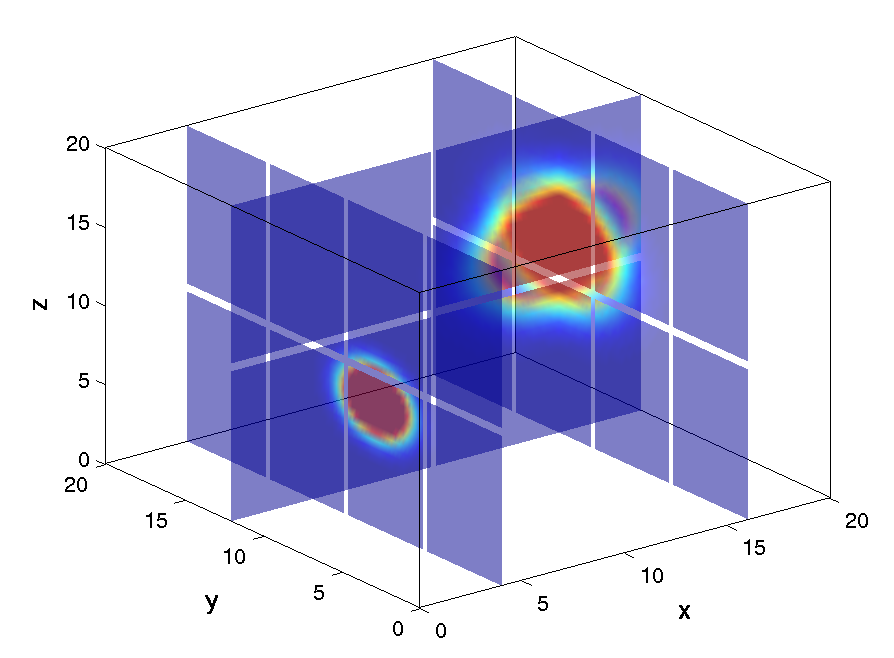
\epsfig{file=pvakx3Dcf.eps,width=0.75\textwidth}}}
  \caption{Results for the \id{pvakx} example problem in 3D.
  Nominal values of the source parameters.}\label{f:pvakx3D_a}
\end{figure}
%%
\begin{figure}
  {\centerline{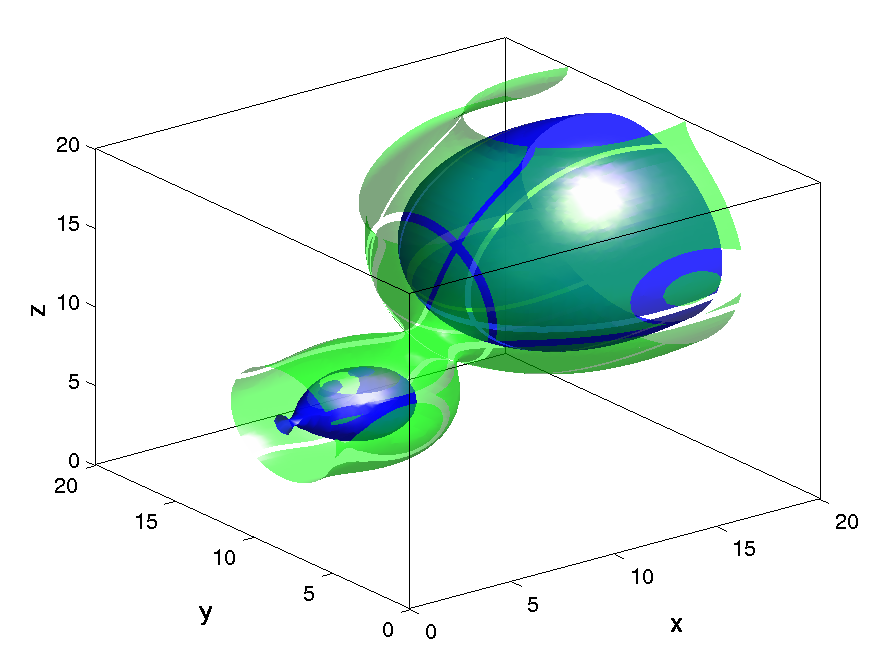
\epsfig{file=pvakx3Dgrad.eps,width=0.75\textwidth}}}
  \caption{Results for the \id{pvakx} example problem in 3D.
  Two isosurfaces of the gradient with respect to the source parameters.
  They correspond to values of $0.25$ (green) and $0.4$ (blue).}\label{f:pvakx3D_b}  
\end{figure}
%%
A sample output generated by \id{pvakx} for a 2D calculation is shown below.

\includeOutput{pvakx}{../examples_par/pvakx.out}


%===============================================================
% Types realtype and integertype
\include{cvs_types}
%===============================================================
% Description of the NVECTOR Concept
%===================================================================================
\chapter{Description of the NVECTOR module}\label{s:nvector}
%===================================================================================
\index{NVECTOR@\texttt{NVECTOR} module}
% This is a shared SUNDIALS TEX file with description of
% the generic nvector abstraction
%
The {\sundials} solvers are written in a data-independent manner. 
They all operate on generic vectors (of type \Id{N\_Vector}) through a set of
operations defined by the particular {\nvector} implementation.
Users can provide their own specific implementation of the {\nvector}
module, or use one of the implementations provided with {\sundials}.
The generic operations are described below and the implementations
provided with {\sundials} are described in the following sections.

The generic \ID{N\_Vector} type is a pointer to a structure that has an 
implementation-dependent {\em content} field containing the 
description and actual data of the vector, and an {\em ops} field 
pointing to a structure with generic vector operations.
The type \id{N\_Vector} is defined as
%%
%%
\begin{verbatim}
typedef struct _generic_N_Vector *N_Vector;

struct _generic_N_Vector {
    void *content;
    struct _generic_N_Vector_Ops *ops;
};
\end{verbatim}
%%
%%
The \id{\_generic\_N\_Vector\_Ops} structure is essentially a list of pointers to
the various actual vector operations, and is defined as
%%
\begin{verbatim}
struct _generic_N_Vector_Ops {
  N_Vector_ID (*nvgetvectorid)(N_Vector);
  N_Vector    (*nvclone)(N_Vector);
  N_Vector    (*nvcloneempty)(N_Vector);
  void        (*nvdestroy)(N_Vector);
  void        (*nvspace)(N_Vector, sunindextype *, sunindextype *);
  realtype*   (*nvgetarraypointer)(N_Vector);
  void        (*nvsetarraypointer)(realtype *, N_Vector);
  void        (*nvlinearsum)(realtype, N_Vector, realtype, N_Vector, N_Vector); 
  void        (*nvconst)(realtype, N_Vector);
  void        (*nvprod)(N_Vector, N_Vector, N_Vector);
  void        (*nvdiv)(N_Vector, N_Vector, N_Vector);
  void        (*nvscale)(realtype, N_Vector, N_Vector);
  void        (*nvabs)(N_Vector, N_Vector);
  void        (*nvinv)(N_Vector, N_Vector);
  void        (*nvaddconst)(N_Vector, realtype, N_Vector);
  realtype    (*nvdotprod)(N_Vector, N_Vector);
  realtype    (*nvmaxnorm)(N_Vector);
  realtype    (*nvwrmsnorm)(N_Vector, N_Vector);
  realtype    (*nvwrmsnormmask)(N_Vector, N_Vector, N_Vector);
  realtype    (*nvmin)(N_Vector);
  realtype    (*nvwl2norm)(N_Vector, N_Vector);
  realtype    (*nvl1norm)(N_Vector);
  void        (*nvcompare)(realtype, N_Vector, N_Vector);
  booleantype (*nvinvtest)(N_Vector, N_Vector);
  booleantype (*nvconstrmask)(N_Vector, N_Vector, N_Vector);
  realtype    (*nvminquotient)(N_Vector, N_Vector);
  int         (*nvlinearcombination)(int, realtype*, N_Vector*, N_Vector);
  int         (*nvscaleaddmulti)(int, realtype*, N_Vector, N_Vector*, N_Vector*);
  int         (*nvdotprodmulti)(int, N_Vector, N_Vector*, realtype*);
  int         (*nvlinearsumvectorarray)(int, realtype, N_Vector*, realtype,
                                        N_Vector*, N_Vector*);
  int         (*nvscalevectorarray)(int, realtype*, N_Vector*, N_Vector*);
  int         (*nvconstvectorarray)(int, realtype, N_Vector*);
  int         (*nvwrmsnomrvectorarray)(int, N_Vector*, N_Vector*, realtype*);
  int         (*nvwrmsnomrmaskvectorarray)(int, N_Vector*, N_Vector*, N_Vector,
                                           realtype*);
  int         (*nvscaleaddmultivectorarray)(int, int, realtype*, N_Vector*,
                                            N_Vector**, N_Vector**);
  int         (*nvlinearcombinationvectorarray)(int, int, realtype*, N_Vector**,
                                                N_Vector*);
};
\end{verbatim}




The generic {\nvector} module defines and implements the vector operations 
acting on an \id{N\_Vector}.
These routines are nothing but wrappers for the vector operations defined by
a particular {\nvector} implementation, which are accessed through the {\em ops}
field of the \id{N\_Vector} structure. To illustrate this point we
show below the implementation of a typical vector operation from the
generic {\nvector} module, namely \id{N\_VScale}, which performs the scaling of a
vector \id{x} by a scalar \id{c}:
%%
%%
\begin{verbatim}
void N_VScale(realtype c, N_Vector x, N_Vector z) 
{
   z->ops->nvscale(c, x, z);
}
\end{verbatim}
%%
%%
Table \ref{t:nvecops} contains a complete list of all standard vector operations defined
by the generic {\nvector} module. Tables \ref{t:nvecfusedops} and \ref{t:nvecarrayops}
list \textit{optional} fused and vector array operations respectively.

Fused and vector array operations are intended to increase data reuse, reduce
parallel communication on distributed memory systems, and lower the number of
kernel launches on systems with accelerators. If a particular {\nvector}
implementation defines a fused or vector array operation as \id{NULL}, the
generic {\nvector} module will automatically call standard vector operations as
necessary to complete the desired operation. Currently, all fused and vector
array operations are disabled by default however, {\sundials} provided {\nvector}
implementations define additional user-callable functions to enable/disable
any or all of the fused and vector array operations. See the following sections
for the implementation specific functions to enable/disable operations.

Finally, note that the generic {\nvector} module defines the functions
\ID{N\_VCloneVectorArray} and \ID{N\_VCloneVectorArrayEmpty}.  Both functions
create (by cloning) an array of \id{count} variables of type \id{N\_Vector}, each
of the same type as an existing \id{N\_Vector}. Their prototypes are
\begin{verbatim}
N_Vector *N_VCloneVectorArray(int count, N_Vector w);
N_Vector *N_VCloneVectorArrayEmpty(int count, N_Vector w);
\end{verbatim}
and their definitions are based on the implementation-specific \id{N\_VClone} and
\id{N\_VCloneEmpty} operations, respectively.

An array of variables of type \id{N\_Vector} can be destroyed by
calling \ID{N\_VDestroyVectorArray}, whose prototype is
\begin{verbatim}
void N_VDestroyVectorArray(N_Vector *vs, int count);
\end{verbatim}
and whose definition is based on the implementation-specific \id{N\_VDestroy} operation.


A particular implementation of the {\nvector} module must:
\begin{itemize}
\item Specify the {\em content} field of \id{N\_Vector}.
\item Define and implement the vector operations. 
  Note that the names of these routines should be unique to that implementation in order 
  to permit using more than one {\nvector} module (each with different \id{N\_Vector} 
  internal data representations) in the same code.
\item Define and implement user-callable constructor and destructor
  routines to create and free an \id{N\_Vector} with
  the new {\em content} field and with {\em ops} pointing to the
  new vector operations.
\item Optionally, define and implement additional user-callable routines
  acting on the newly defined \id{N\_Vector} (e.g., a routine to print
  the content for debugging purposes).
\item Optionally, provide accessor macros as needed for that particular implementation to 
  be used to access different parts in the {\em content} field of the newly defined \id{N\_Vector}.
\end{itemize}

Each {\nvector} implementation included in {\sundials} has a unique 
identifier specified in enumeration and shown in Table \ref{t:vectorIDs}.
It is recommended that a user-supplied {\nvector} implementation use the 
\id{SUNDIALS\_NVEC\_CUSTOM} identifier.

\begin{table}
\centering
\caption{Vector Identifications associated with vector kernels supplied with \id{\sundials}.}
\label{t:vectorIDs}
\medskip
\begin{tabular}{|l|l|c|}
\hline
{\bf Vector ID} & {\bf Vector type} & {\bf ID Value} \\
\hline
SUNDIALS\_NVEC\_SERIAL     & Serial                            & 0 \\ 
SUNDIALS\_NVEC\_PARALLEL   & Distributed memory parallel (MPI) & 1 \\
SUNDIALS\_NVEC\_OPENMP     & OpenMP shared memory parallel     & 2 \\
SUNDIALS\_NVEC\_PTHREADS   & PThreads shared memory parallel   & 3 \\
SUNDIALS\_NVEC\_PARHYP     & {\hypre} ParHyp parallel vector   & 4 \\ 
SUNDIALS\_NVEC\_PETSC      & {\petsc} parallel vector          & 5 \\
SUNDIALS\_NVEC\_CUSTOM     & User-provided custom vector       & 6 \\
\hline
\end{tabular}
\end{table}

%% \begin{verbatim}
%% typedef enum {
%%   SUNDIALS_NVEC_SERIAL, 
%%   SUNDIALS_NVEC_PARALLEL, 
%%   SUNDIALS_NVEC_OPENMP, 
%%   SUNDIALS_NVEC_PTHREADS, 
%%   SUNDIALS_NVEC_PARHYP, 
%%   SUNDIALS_NVEC_PETSC,
%%   SUNDIALS_NVEC_CUSTOM
%% } N_Vector_ID; 
%% \end{verbatim}

%---------------------------------------------------------------------------
% Table of vector kernels
%---------------------------------------------------------------------------
\newpage

\newlength{\colone}
\settowidth{\colone}{\id{N\_VGetArrayPointer}}
\newlength{\coltwo}
\setlength{\coltwo}{\textwidth}
\addtolength{\coltwo}{-0.4in}
\addtolength{\coltwo}{-\colone}

\tablecaption{Description of the NVECTOR operations}\label{t:nvecops}
\tablefirsthead{\hline {\rule{0mm}{5mm}}{\bf Name} & {\bf Usage and Description} \\[3mm] \hline\hline}
\tablehead{\hline \multicolumn{2}{|l|}{\small\slshape continued from last page} \\
           \hline {\rule{0mm}{5mm}}{\bf Name} & {\bf Usage and  Description} \\[3mm] \hline\hline}
\tabletail{\hline \multicolumn{2}{|r|}{\small\slshape continued on next page} \\ \hline}
\tablelasttail{\hline}
\begin{xtabular}{|p{\colone}|p{\coltwo}|}
%%
\id{N\_VGetVectorID} & \id{id = N\_VGetVectorID(w);} \\ 
& Returns the vector type identifier for the vector \id{w}. It is used to determine the
vector implementation type (e.g.~serial, parallel,\ldots) from the abstract 
\id{N\_Vector} interface.  Returned values are given in Table \ref{t:vectorIDs}.
\\[2mm]
%%
\id{N\_VClone} & \id{v = N\_VClone(w);} \\ 
& Creates a new \id{N\_Vector} of the same type as an existing vector \id{w} and sets the
{\em ops} field.
It does not copy the vector, but rather allocates storage for the new vector.
\\[2mm]
%%
\id{N\_VCloneEmpty} & \id{v = N\_VCloneEmpty(w);} \\ 
& Creates a new \id{N\_Vector} of the same type as an existing vector \id{w} and sets the
{\em ops} field.
It does not allocate storage for data.
\\[2mm]
%%
\id{N\_VDestroy} & \id{N\_VDestroy(v);} \\
& Destroys the \id{N\_Vector} \id{v} and frees memory allocated for its
internal data.
\\[2mm]
%%
\id{N\_VSpace} & \id{N\_VSpace(nvSpec, \&lrw, \&liw);} \\
& Returns storage requirements for one \id{N\_Vector}.
\id{lrw} contains the number of realtype words and \id{liw}
contains the number of integer words.
This function is advisory only, for use in determining a user's total
space requirements; it could be a dummy function in a user-supplied
{\nvector} module if that information is not of interest.
\\[2mm]
%%
\id{N\_VGetArrayPointer} & \id{vdata = N\_VGetArrayPointer(v);} \\
& Returns a pointer to a \id{realtype} array from the \id{N\_Vector} \id{v}.
Note that this assumes that the internal data in \id{N\_Vector} is
a contiguous array of \id{realtype}.
This routine is only used in the solver-specific interfaces to the dense and
banded (serial) linear solvers, the sparse linear solvers (serial and
threaded), and in the interfaces to the banded (serial)
and band-block-diagonal (parallel) preconditioner modules provided with {\sundials}.
\\[2mm]
%%
\id{N\_VSetArrayPointer} & \id{N\_VSetArrayPointer(vdata, v);} \\
& Overwrites the data in an \id{N\_Vector} with a given array of \id{realtype}.
Note that this assumes that the internal data in \id{N\_Vector} is
a contiguous array of \id{realtype}.
This routine is only used in the interfaces to the dense (serial) linear
solver, hence need not exist in a user-supplied {\nvector} module for a
parallel environment.
\\[2mm]
%%
\id{N\_VLinearSum} & \id{N\_VLinearSum(a, x, b, y, z);} \\
& Performs the operation $z = a x + b y$, where $a$ and $b$ are \id{realtype} 
scalars and $x$ and $y$ are of type \id{N\_Vector}:
$z_i = a x_i + b y_i, \: i=0,\ldots,n-1$.
\\[2mm]
%%
\id{N\_VConst} & \id{N\_VConst(c, z);} \\
& Sets all components of the \id{N\_Vector} \id{z} to \id{realtype} \id{c}:
$z_i = c,\: i=0,\ldots,n-1$.
\\[2mm]
%%
\id{N\_VProd} & \id{N\_VProd(x, y, z);} \\
& Sets the \id{N\_Vector} \id{z} to be the component-wise product of the
\id{N\_Vector} inputs \id{x} and \id{y}:
$z_i = x_i y_i,\: i=0,\ldots,n-1$.
\\[2mm]
%%
\id{N\_VDiv} & \id{N\_VDiv(x, y, z);} \\
& Sets the \id{N\_Vector} \id{z} to be the component-wise ratio of the
\id{N\_Vector} inputs \id{x} and \id{y}:
$z_i = x_i / y_i,\: i=0,\ldots,n-1$. The $y_i$ may not be tested 
for $0$ values. It should only be called with a \id{y} that is
guaranteed to have all nonzero components.
\\[2mm]
%%
\id{N\_VScale} & \id{N\_VScale(c, x, z);} \\
& Scales the \id{N\_Vector} \id{x} by the \id{realtype} scalar \id{c} 
and returns the result in \id{z}:
$z_i = c x_i , \: i=0,\ldots,n-1$.
\\[2mm]
%%
\id{N\_VAbs} & \id{N\_VAbs(x, z);} \\
& Sets the components of the \id{N\_Vector} \id{z} to be the absolute
values of the components of the \id{N\_Vector} \id{x}:
$y_i = | x_i | , \: i=0,\ldots,n-1$.
\\[2mm]
%%
\id{N\_VInv} & \id{N\_VInv(x, z);} \\
& Sets the components of the \id{N\_Vector} \id{z} to be the inverses
of the components of the \id{N\_Vector} \id{x}:
$z_i = 1.0 /  x_i  , \: i=0,\ldots,n-1$. This routine
may not check for division by $0$. It should be called only with an 
\id{x} which is guaranteed to have all nonzero components.
\\[2mm]
%%
\id{N\_VAddConst} & \id{N\_VAddConst(x, b, z);} \\
& Adds the \id{realtype} scalar \id{b} to all components of \id{x} 
and returns the result in the \id{N\_Vector} \id{z}:
$z_i = x_i + b , \: i=0,\ldots,n-1$.
\\[2mm]
%%
\id{N\_VDotProd} & \id{d = N\_VDotProd(x, y);} \\
& Returns the value of the ordinary dot product of \id{x} and \id{y}:
$d=\sum_{i=0}^{n-1} x_i y_i$.
\\[2mm]
%%
\id{N\_VMaxNorm} & \id{m = N\_VMaxNorm(x);} \\
& Returns the maximum norm of the \id{N\_Vector} \id{x}:
$m = \max_{i} | x_i |$.
\\[2mm]
%%
\id{N\_VWrmsNorm} & \id{m = N\_VWrmsNorm(x, w)} \\
& Returns the weighted root-mean-square norm of the \id{N\_Vector} \id{x} with
\id{realtype} weight vector \id{w}:
$m = \sqrt{\left( \sum_{i=0}^{n-1} (x_i w_i)^2 \right) / n}$.
\\[2mm]
%%
\id{N\_VWrmsNormMask} & \id{m = N\_VWrmsNormMask(x, w, id);} \\
& Returns the weighted root mean square norm of the \id{N\_Vector} \id{x} with
\id{realtype} weight vector \id{w} built using only 
the elements of \id{x} corresponding to
positive elements of the \id{N\_Vector} \id{id}:\\
&$m = \sqrt{\left( \sum_{i=0}^{n-1} (x_i w_i H(id_i))^2 \right) / n}$,
where
$
H(\alpha) =
\begin{cases} 
1 & \alpha > 0 \\
0 & \alpha \leq 0
\end{cases}
$
\\[2mm]
%%
\id{N\_VMin} & \id{m = N\_VMin(x);} \\
& Returns the smallest element of the \id{N\_Vector} \id{x}:
$m = \min_i x_i $.
\\[2mm]
%%
\id{N\_VWL2Norm} & \id{m = N\_VWL2Norm(x, w);} \\
& Returns the weighted Euclidean $\ell_2$ norm of the \id{N\_Vector} \id{x}
with \id{realtype} weight vector \id{w}: 
$m = \sqrt{\sum_{i=0}^{n-1} (x_i w_i)^2}$.
\\[2mm]
%%
\id{N\_VL1Norm} & \id{m = N\_VL1Norm(x);} \\
& Returns the $\ell_1$ norm of the \id{N\_Vector} \id{x}:
$m = \sum_{i=0}^{n-1} | x_i |$.
\\[2mm]
%%
\id{N\_VCompare} & \id{N\_VCompare(c, x, z);} \\
& Compares the components of the \id{N\_Vector} \id{x} to the \id{realtype}
scalar \id{c} and returns an \id{N\_Vector} \id{z} such that:
$z_i = 1.0$ if $| x_i | \ge c$ and $z_i = 0.0$ otherwise.
\\[2mm]
%%
\id{N\_VInvTest} & \id{t = N\_VInvTest(x, z);} \\
& Sets the components of the \id{N\_Vector} \id{z} to be the inverses
of the components of the \id{N\_Vector} \id{x}, with prior testing
for zero values:
$z_i = 1.0 /  x_i  , \: i=0,\ldots,n-1$.
This routine returns a boolean assigned to \id{SUNTRUE} if all 
components of \id{x} are
nonzero (successful inversion) and returns \id{SUNFALSE} otherwise.  
\\[2mm]
%%
\id{N\_VConstrMask} & \id{t = N\_VConstrMask(c, x, m);} \\
& Performs the following constraint tests:
$x_i > 0$ if $c_i=2$,
$x_i \ge 0$ if $c_i=1$,
$x_i \le 0$ if $c_i=-1$,
$x_i < 0$ if $c_i=-2$.
There is no constraint on $x_i$ if $c_i=0$.
This routine returns a boolean assigned to \id{SUNFALSE} if any element failed
the constraint test and assigned to \id{SUNTRUE} if all passed.  It also sets a
mask vector \id{m}, with elements equal to $1.0$ where the constraint 
test failed, and $0.0$ where the test passed.
This routine is used only for constraint checking.
\\[2mm]
%%
\id{N\_VMinQuotient} & \id{minq = N\_VMinQuotient(num, denom);} \\
& This routine returns the minimum of the quotients obtained   
by term-wise dividing \id{num}$_i$ by \id{denom}$_i$. 
A zero element in \id{denom} will be skipped. 
If no such quotients are found, then the large value 
\Id{BIG\_REAL} (defined in the header file \id{sundials\_types.h})
is returned. 
\\
%%
\end{xtabular}
\bigskip

%---------------------------------------------------------------------------
% Table of fused vector kernels
%---------------------------------------------------------------------------
%\newpage

\newlength{\coloneb}
\settowidth{\coloneb}{\id{N\_VLinearCombination}}
\newlength{\coltwob}
\setlength{\coltwob}{\textwidth}
\addtolength{\coltwob}{-0.4in}
\addtolength{\coltwob}{-\coloneb}

\tablecaption{Description of the NVECTOR fused operations}\label{t:nvecfusedops}
\tablefirsthead{\hline {\rule{0mm}{5mm}}{\bf Name} & {\bf Usage and Description} \\[3mm] \hline\hline}
\tablehead{\hline \multicolumn{2}{|l|}{\small\slshape continued from last page} \\
           \hline {\rule{0mm}{5mm}}{\bf Name} & {\bf Usage and  Description} \\[3mm] \hline\hline}
\tabletail{\hline \multicolumn{2}{|r|}{\small\slshape continued on next page} \\ \hline}
\tablelasttail{\hline}
\begin{xtabular}{|p{\coloneb}|p{\coltwob}|}
%%
\id{N\_VLinearCombination} & \id{ier = N\_VLinearCombination(nv, c, X, z);} \\ 
& This routine computes the linear combination of $n_v$ vectors with $n$
elements:
\begin{equation*}
z_i = \sum_{j=0}^{n_v-1} c_j x_{j,i}, \quad i=0,\ldots,n-1,
\end{equation*}
where $c$ is an array of $n_v$ scalars (type \id{realtype}*), $X$ is an array of
$n_v$ vectors (type \id{N\_Vector*}), and $z$ is the output vector (type
\id{N\_Vector}). If the output vector $z$ is one of the vectors in $X$, then it
\textit{must} be the first vector in the vector array. The operation returns
\id{0} for success and a non-zero value otherwise.
\\[2mm]
%%
\id{N\_VScaleAddMulti} & \id{ier = N\_VScaleAddMulti(nv, c, x, Y, Z);} \\ 
& This routine scales and adds one vector to $n_v$ vectors with $n$ elements:
\begin{equation*}
z_{j,i} = c_j x_i + y_{j,i}, \quad j=0,\ldots,n_v-1 \quad i=0,\ldots,n-1,
\end{equation*}
where $c$ is an array of $n_v$ scalars (type \id{realtype}*), $x$ is the vector
(type \id{N\_Vector}) to be scaled and added to each vector in the vector array
of $n_v$ vectors $Y$ (type \id{N\_Vector*}), and $Z$ (type \id{N\_Vector*}) is a
vector array of $n_v$ output vectors. The operation returns \id{0} for success and a
non-zero value otherwise.
\\[2mm]
%%
\id{N\_VDotProdMulti} & \id{ier = N\_VDotProdMulti(nv, x, Y, d);} \\ 
& This routine computes the dot product of a vector with $n_v$ other vectors:
\begin{equation*}
d_j = \sum_{i=0}^{n-1} x_i y_{j,i}, \quad j=0,\ldots,n_v-1,
\end{equation*}
where $d$ (type \id{realtype}*) is an array of $n_v$ scalars containing the
dot products of the vector $x$ (type \id{N\_Vector}) with each of the $n_v$
vectors in the vector array $Y$ (type \id{N\_Vector*}). The operation returns
\id{0} for success and a non-zero value otherwise.
\\
%%
\end{xtabular}
\bigskip

%---------------------------------------------------------------------------
% Table of vector array kernels
%---------------------------------------------------------------------------
%\newpage

\newlength{\colonec}
\settowidth{\colonec}{\id{N\_VLinearCombinationVectorArray}}
\newlength{\coltwoc}
\setlength{\coltwoc}{\textwidth}
\addtolength{\coltwoc}{-0.4in}
\addtolength{\coltwoc}{-\colonec}

\tablecaption{Description of the NVECTOR vector array operations}\label{t:nvecarrayops}
\tablefirsthead{\hline {\rule{0mm}{5mm}}{\bf Name} & {\bf Usage and Description} \\[3mm] \hline\hline}
\tablehead{\hline \multicolumn{2}{|l|}{\small\slshape continued from last page} \\
           \hline {\rule{0mm}{5mm}}{\bf Name} & {\bf Usage and  Description} \\[3mm] \hline\hline}
\tabletail{\hline \multicolumn{2}{|r|}{\small\slshape continued on next page} \\ \hline}
\tablelasttail{\hline}
\begin{xtabular}{|p{\colonec}|p{\coltwoc}|}
%%
\id{N\_VLinearSumVectorArray} & \id{ier = N\_VLinearSumVectorArray(nv, a, X, b, Y, Z);} \\
& This routine comuptes the linear sum of two vector arrays containing $n_v$
vectors of $n$ elements:
\begin{equation*}
z_{j,i} = a x_{j,i} + b y_{j,i}, \quad i=0,\ldots,n-1 \quad j=0,\ldots,n_v-1,
\end{equation*}
where $a$ and $b$ are \id{realtype} scalars and $X$, $Y$, and $Z$ are arrays of
$n_v$ vectors (type \id{N\_Vector*}). The operation returns \id{0} for success and
a non-zero value otherwise.
\\[2mm]
%%
\id{N\_VScaleVectorArray} & \id{ier = N\_VScaleVectorArray(nv, c, X, Z);} \\
& This routine scales each vector of $n$ elements in a vector array of $n_v$
vectors by a potentially different constant:
\begin{equation*}
z_{j,i} = c_j x_{j,i}, \quad i=0,\ldots,n-1 \quad j=0,\ldots,n_v-1,
\end{equation*}
where $c$ is an array of $n_v$ scalars (type \id{realtype}*) and $X$ and $Z$ are
arrays of $n_v$ vectors (type \id{N\_Vector*}). The operation returns \id{0} for
success and a non-zero value otherwise.
\\[2mm]
%%
\id{N\_VConstVectorArray} & \id{ier = N\_VConstVectorArray(nv, c, X);} \\
& This routine sets each element in a vector of $n$ elements in a vector array of
$n_v$ vectors to the same value:
\begin{equation*}
z_{j,i} = c, \quad i=0,\ldots,n-1 \quad j=0,\ldots,n_v-1,
\end{equation*}
where $c$ is a \id{realtype} scalar and $X$ is an array of $n_v$ vectors (type
\id{N\_Vector*}). The operation returns \id{0} for success and a non-zero value
otherwise.
\\[2mm]
%%
\id{N\_VWrmsNormVectorArray} & \id{ier = N\_VWrmsNormVectorArray(nv, X, W, m);} \\
& This routine computes the weighted root mean square norm of $n_v$ vectors with
$n$ elements:
\begin{equation*}
m_j = \left( \frac1n \sum_{i=0}^{n-1} \left(x_{j,i} w_{j,i}\right)^2\right)^{1/2}, \quad j=0,\ldots,n_v-1,
\end{equation*}
where $m$ (type \id{realtype*}) contains the $n_v$ norms of the vectors in the
vector array $X$ (type \id{N\_Vector*}) with corresponding weight vectors $W$
(type \id{N\_Vector*}). The operation returns \id{0} for success and a non-zero
value otherwise.
\\[2mm]
%%
\id{N\_VWrmsNormMaskVectorArray} & \id{ier = N\_VWrmsNormMaskVectorArray(nv, X, W, id, m);} \\
& This routine computes the masked weighted root mean square norm of $n_v$
vectors with $n$ elements:
\begin{equation*}
m_j = \left( \frac1n \sum_{i=0}^{n-1} \left(x_{j,i} w_{j,i}
H(id_i)\right)^2 \right)^{1/2}, \quad j=0,\ldots,n_v-1,
\end{equation*}
$H(id_i)=1$ for $id_i > 0$ and is zero otherwise, $m$ (type \id{realtype*}) contains
the $n_v$ norms of the vectors in the vector array $X$ (type \id{N\_Vector*}) with
corresponding weight vectors $W$ (type \id{N\_Vector*}) and mask vector $id$
(type \id{N\_Vector}). The operation returns \id{0} for success and a non-zero
value otherwise.
\\[2mm]
%%
\id{N\_VScaleAddMultiVectorArray} & \id{ier = N\_VScaleAddMultiVectorArray(nv, ns, c, X, YY, ZZ);} \\ 
& This routine scales and adds a vector in a vector array of $n_v$ vectors to
the corresponding vector in $n_s$ vector arrays:
\begin{equation*}
z_{j,i} = \sum_{k=0}^{n_s-1} c_k x_{k,j,i}, \quad i=0,\ldots,n-1 \quad j=0,\ldots,n_v-1,
\end{equation*}
where $c$ is an array of $n_s$ scalars (type \id{realtype*}), $X$ is a vector
array of $n_v$ vectors (type id{N\_Vector*}) to be scaled and added to the
corresponding vector in each of the $n_s$ vector arrays in the array of vector
arrays $YY$ (type \id{N\_Vector**}) and stored in the output array of vector
arrays $ZZ$ (type \id{N\_Vector**}). The operation returns \id{0} for success
and a non-zero value otherwise.
\\[2mm]
%%
\id{N\_VLinearCombinationVectorArray} & \id{ier = N\_VLinearCombinationVectorArray(nv, ns, c, XX, Z);} \\ 
& This routine computes the linear combination of $n_s$ vector arrays containing
$n_v$ vectors with $n$ elements:
\begin{equation*}
z_{j,i} = \sum_{k=0}^{n_s-1} c_k x_{k,j,i}, \quad i=0,\ldots,n-1 \quad j=0,\ldots,n_v-1,
\end{equation*}
where $c$ is an array of $n_s$ scalars (type \id{realtype*}), $XX$
(type \id{N\_Vector**}) is an array of $n_s$ vector arrays each containing $n_v$
vectors to be summed into the output vector array of $n_v$ vectors $Z$ (type
\id{N\_Vector*}). If the output vector array $Z$ is one of the vector arrays in
$XX$, then it \textit{must} be the first vector array in $XX$. The operation
returns \id{0} for success and a non-zero value otherwise.
\\
%%
\end{xtabular}

%---------------------------------------------------------------------------
\section{The NVECTOR\_SERIAL implementation}\label{ss:nvec_ser}
%% This is a shared SUNDIALS TEX file with description of
%% the serial nvector implementation
%%

The {\nvecs} implementation of the {\nvector} module defines the {\em content} 
field of \id{N\_Vector} to be a structure containing the length of the vector 
and a pointer to the beginning of a contiguous data array.
%%
\begin{verbatim} 
struct _N_VectorContent_Serial {
  long int length;
  realtype *data;
};
\end{verbatim}
%%
%%--------------------------------------------
%%
The following four macros are provided to access the content of a {\nvecs}
vector. The suffix \id{\_S} in the names denotes serial version.
%%
\begin{itemize}

\item \ID{NV\_CONTENT\_S}                             
    
  This routine gives access to the contents of the serial
  vector \id{N\_Vector}.
  
  The assignment \id{v\_cont} $=$ \id{NV\_CONTENT\_S(v)} sets           
  \id{v\_cont} to be a pointer to the serial \id{N\_Vector} content  
  structure.                                             
                                                            
  Implementation: 
  
  \verb|#define NV_CONTENT_S(v) ( (N_VectorContent_Serial)(v->content) )|
  
\item \ID{NV\_DATA\_S}, \ID{NV\_LENGTH\_S}                                 
                                                            
  These macros give individual access to the parts of    
  the content of a serial \id{N\_Vector}.                        
                                                               
  The assignment \id{v\_data = NV\_DATA\_S(v)} sets \id{v\_data} to be     
  a pointer to the first component of the data for the \id{N\_Vector} \id{v}. 
  The assignment \id{NV\_DATA\_S(v) = v\_data} sets the component array of \id{v} to     
  be \id{v\_data} by storing the pointer \id{v\_data}.                   
  
  The assignment \id{v\_len = NV\_LENGTH\_S(v)} sets \id{v\_len} to be     
  the length of \id{v}. On the other hand, the call \id{NV\_LENGTH\_S(v) = len\_v} 
  sets the length of \id{v} to be \id{len\_v}.
                                                            
  Implementation: 
  
  \verb|#define NV_DATA_S(v) ( NV_CONTENT_S(v)->data )|
  
  \verb|#define NV_LENGTH_S(v) ( NV_CONTENT_S(v)->length )|

\item \ID{NV\_Ith\_S}                                               
                                                            
  This macro gives access to the individual components of the data
  array of an \id{N\_Vector}.

  The assignment \id{r = NV\_Ith\_S(v,i)} sets \id{r} to be the value of 
  the \id{i}-th component of \id{v}. The assignment \id{NV\_Ith\_S(v,i) = r}   
  sets the value of the \id{i}-th component of \id{v} to be \id{r}.        
  
  Here $i$ ranges from $0$ to $n-1$ for a vector of length $n$.

  Implementation:

  \verb|#define NV_Ith_S(v,i) ( NV_DATA_S(v)[i] )|

\end{itemize}
%%
%%----------------------------------------------
%%
The {\nvecs} module defines serial implementations of all vector operations listed 
in Table \ref{t:nvecops} and provides the following user-callable routines:
%%
\begin{itemize}

\item \ID{N\_VNew\_Serial}

  This function creates and allocates memory for a serial \id{N\_Vector}.
  Its only argument is the vector length.

  Prototype

  \verb|N_Vector N_VNew_Serial(long int vec_length);|

\item \ID{N\_VNewEmpty\_Serial}

  This function creates a new serial \id{N\_Vector} with an empty (\id{NULL}) data array.

  Prototype

  \verb|N_Vector N_VNewEmpty_Serial(long int vec_length);|

\item \ID{N\_VMake\_Serial}

 This function creates and allocates memory for a serial vector
 with user-provided data array.

 Prototype

 \verb|N_Vector N_VMake_Serial(long int vec_length, realtype *v_data);|


\item \ID{N\_VNewVectorArray\_Serial}

 This function creates an array of \id{count} serial vectors.
 This array of \id{N\_Vector} can be freed with \id{N\_VDestroyVectorArray}
 (defined by the generic nvector module).

 Prototype

 \verb|N_Vector *N_VNewVectorArray_Serial(int count, long int vec_length);|


\item \ID{N\_VDispose\_Serial}

 This function frees a serial \id{N\_Vector} created with \id{N\_VMake\_Serial}.
 Note that deallocation of the {\em data} array is the user's
 responsibility. In other words, \id{N\_VDispose\_Serial} is identitical
 to \id{N\_VDestroyEmpty\_Serial} (defined by {\nvecs} as part of the {\em ops}
 structure).

 Prototype

 \verb|void N_VDispose_Serial(N_Vector v);|


\item \ID{N\_VPrint\_Serial}

 This function prints the content of a serial vector to \id{stdout}.

 Prototype
 
 \verb|void N_VPrint_Serial(N_Vector v);|

\end{itemize}
%%
%%------------------------------------
%%
\paragraph{\bf Notes}                                                      
           
\begin{itemize}
                                        
\item
  When looping over the components of an \id{N\_Vector} \id{v}, it is     
  more efficient to first obtain the component array via       
  \id{v\_data = NV\_DATA\_S(v)} and then access \id{v\_data[i]} within the     
  loop than it is to use \id{NV\_Ith\_S(v,i)} within the loop.        
                                     
\item                          
  \id{NV\_MAKE\_S} and \id{NV\_DISPOSE\_S} are similar to the \id{N\_VNew} and  
  \id{N\_VFree} implemented by {\nvecs}, while \id{NVS\_MAKE\_S} and 
  \id{NVS\_DISPOSE\_S}  are similar to  \id{N\_VNew\_S} and \id{N\_VFree\_S}. 
  The difference is one of responsibility for component memory     
  allocation and deallocation. \id{N\_VNew} allocates memory  
  for the \id{N\_Vector} components and \id{N\_VFree} frees the     
  component memory allocated by \id{N\_VNew}. For \id{NV\_MAKE\_S}   
  and \id{NV\_DISPOSE\_S}, the component memory is allocated and      
  freed by the user of this package. Similar remarks hold for  
  \id{NVS\_MAKE\_S},  \id{NVS\_DISPOSE\_S} and \id{N\_VNew\_S},              
  \id{N\_VFree\_S}.                                            

\item
  To maximize efficiency, vector operations in the {\nvecs} implementation
  that have more than one \id{N\_Vector} argument do not check for
  consistent internal representation of these vectors. It is the user's 
  responsibility to ensure that such routines are called with \id{N\_Vector}
  arguments that were all created with the \id{NV\_Spec} structure returned
  by \id{NV\_SpecInit\_Serial}.

\end{itemize}


%---------------------------------------------------------------------------
\section{The NVECTOR\_PARALLEL implementation}\label{ss:nvec_par}
% This is a shared SUNDIALS TEX file with description of
% the parallel nvector implementation
%
The parallel implementation of the {\nvector} module provided with {\sundials},
{\nvecp}, defines the {\em content} 
field of \id{N\_Vector} to be a structure containing the global and local lengths 
of the vector, a pointer to the beginning of a contiguous local data array,
an {\mpi} communicator, an a boolean flag {\em own\_data} indicating ownership of 
the data array {\em data}.
%%
\begin{verbatim} 
struct _N_VectorContent_Parallel {
  long int local_length;
  long int global_length;
  booleantype own_data;
  realtype *data;
  MPI_Comm comm;
};
\end{verbatim}
%%
%%--------------------------------------------
%%
The following seven macros are provided to access the content of a {\nvecp}
vector. The suffix \id{\_P} in the names denotes parallel version.
\begin{itemize}

\item 
  \ID{NV\_CONTENT\_P}

  This macro gives access to the contents of the parallel
  vector \id{N\_Vector}.
  
  The assignment \id{v\_cont = NV\_CONTENT\_P(v)} sets       
  \id{v\_cont} to be a pointer to the \id{N\_Vector} content    
  structure of type \id{struct \_N\_VectorParallelContent}.
  
  Implementation:
  
  \verb|#define NV_CONTENT_P(v) ( (N_VectorContent_Parallel)(v->content) )|
  
\item 
  \ID{NV\_OWN\_DATA\_P}, \ID{NV\_DATA\_P}, 
  \ID{NV\_LOCLENGTH\_P}, \ID{NV\_GLOBLENGTH\_P}
  
  These macros give individual access to the parts of    
  the content of a parallel \id{N\_Vector}.                        
  
  The assignment \id{v\_data = NV\_DATA\_P(v)} sets \id{v\_data} to be     
  a pointer to the first component of the local data for the \id{N\_Vector} \id{v}. 
  The assignment \id{NV\_DATA\_P(v) = v\_data} sets the component array of 
  \id{v} to be \id{v\_data} by storing the pointer \id{v\_data}.                   
  
  The assignment \id{v\_llen = NV\_LOCLENGTH\_P(v)} sets \id{v\_llen} to be     
  the length of the local part of \id{v}. 
  The call \id{NV\_LENGTH\_P(v) = llen\_v} sets      
  the local length of \id{v} to be \id{llen\_v}.
  
  The assignment \id{v\_glen = NV\_GLOBLENGTH\_P(v)} sets \id{v\_glen} to  
  be the global length of the vector \id{v}.                    
  The call \id{NV\_GLOBLENGTH\_P(v) = glen\_v} sets the global       
  length of \id{v} to be \id{glen\_v}.
  
  Implementation:
  
  \verb|#define NV_OWN_DATA_P(v)   ( NV_CONTENT_P(v)->own_data )|

  \verb|#define NV_DATA_P(v)       ( NV_CONTENT_P(v)->data )|

  \verb|#define NV_LOCLENGTH_P(v)  ( NV_CONTENT_P(v)->local_length )|

  \verb|#define NV_GLOBLENGTH_P(v) ( NV_CONTENT_P(v)->global_length )|
  
\item \ID{NV\_COMM\_P}

  This macro provides access to the {\mpi} communicator used by the {\nvecp}
  vectors.

  Implementation:

  \verb|#define NV_COMM_P(v) ( NV_CONTENT_P(v)->comm )|

\item \ID{NV\_Ith\_P}

  This macro gives access to the individual components of the local data
  array of an \id{N\_Vector}.

  The assignment \id{r = NV\_Ith\_P(v,i)} sets \id{r} to be the value of 
  the \id{i}-th component of the local part of \id{v}. 
  The assignment \id{NV\_Ith\_P(v,i) = r}   
  sets the value of the \id{i}-th component of the local part of \id{v} 
  to be \id{r}.        
  
  Here $i$ ranges from $0$ to $n-1$, where $n$ is the local length.
      
  Implementation:

  \verb|#define NV_Ith_P(v,i) ( NV_DATA_P(v)[i] )|

\end{itemize}
%%
%%--------------------------------------------
%%
The {\nvecp} module defines parallel implementations of all vector operations listed 
in Table \ref{t:nvecops} and provides the following user-callable routines:
%%
%%
\begin{itemize}

%%--------------------------------------

\item  \ID{N\_VNew\_Parallel}
  
  This function creates and allocates memory for a parallel vector.
 
  

\begin{verbatim}
N_Vector N_VNew_Parallel(MPI_Comm comm, 
                         long int local_length, 
                         long int global_length);
\end{verbatim}
  
%%--------------------------------------

\item \ID{N\_VNewEmpty\_Parallel}
 
  This function creates a new parallel \id{N\_Vector} with an empty (\id{NULL}) data array.
 
  

\begin{verbatim}
N_Vector N_VNewEmpty_Parallel(MPI_Comm comm, 
                              long int local_length, 
                              long int global_length);
\end{verbatim}

  
%%--------------------------------------

\item \ID{N\_VMake\_Parallel}
  
  This function creates and allocates memory for a parallel vector
  with user-provided data array.
 
  

\begin{verbatim}
N_Vector N_VMake_Parallel(MPI_Comm comm, 
                          long int local_length,
                          long int global_length,
                          realtype *v_data);
\end{verbatim}

%%--------------------------------------

\item \ID{N\_VNewVectorArray\_Parallel}
 
  This function creates an array of \id{count} parallel vectors.
 
\begin{verbatim}
N_Vector *N_VNewVectorArray_Parallel(int count, 
                                     MPI_Comm comm, 
                                     long int local_length,
                                     long int global_length);
\end{verbatim}

%%--------------------------------------

\item \ID{N\_VNewVectorArrayEmpty\_Parallel}
 
  This function creates an array of \id{count} parallel vectors,
  each with an empty (\id{NULL}) data array.
 
\begin{verbatim}
N_Vector *N_VNewVectorArrayEmpty_Parallel(int count, 
                                          MPI_Comm comm, 
                                          long int local_length,
                                          long int global_length);
\end{verbatim}

%%--------------------------------------

\item \ID{N\_VDestroyVectorArray\_Parallel}
 
 This function frees memory allocated for the array of \id{count} variables of type \id{N\_Vector}
 created with \id{N\_VNewVectorArray\_Parallel} or with \id{N\_VNewVectorArrayEmpty\_Parallel}.

 

 \verb|void N_VDestroyVectorArray_Parallel(N_Vector *vs, int count);|


%%--------------------------------------

\item \ID{N\_VPrint\_Parallel}
  
  This function prints the content of a parallel vector to stdout.
 
  
  
  \verb|void N_VPrint_Parallel(N_Vector v);|


\end{itemize}
%%
%%------------------------------------
%%
\paragraph{\bf Notes} 
           
\begin{itemize}
                                        
\item
  When looping over the components of an \id{N\_Vector} \id{v}, it is     
  more efficient to first obtain the local component array via       
  \id{v\_data = NV\_DATA\_P(v)} and then access \id{v\_data[i]} within the     
  loop than it is to use \id{NV\_Ith\_P(v,i)} within the loop.        
                                                               
\item
  {\warn} The {\nvecp} constructor functions \id{N\_VNewEmpty\_Parallel}, \id{N\_VMake\_Parallel}, 
  and \id{N\_VNewVectorArrayEmpty\_Parallel}
  set the field {\em own\_data} $=$ \id{FALSE}. 
  The functions \id{N\_VDestroy\_Parallel} and \id{N\_VDestroyVectorArray\_Parallel}
  will not attempt to free the pointer {\em data} for any \id{N\_Vector} with
  {\em own\_data} set to \id{FALSE}. In such a case, it is the user's responsibility to
  deallocate the {\em data} pointer.

\item
  {\warn} To maximize efficiency, vector operations in the {\nvecp} implementation
  that have more than one \id{N\_Vector} argument do not check for
  consistent internal representation of these vectors. It is the user's 
  responsability to ensure that such routines are called with \id{N\_Vector}
  arguments that were all created with the same internal representations.

\end{itemize}



%---------------------------------------------------------------------------
\section{The NVECTOR\_OPENMP implementation}\label{ss:nvec_openmp}
%% This is a shared SUNDIALS TEX file with a description of the
%% OpenMP nvector implementation
%%

The OpenMP implementation of the {\nvector} module provided with {\sundials},
{\nvecopenmp}, defines the {\em content} field of \id{N\_Vector} to be a structure 
containing the length of the vector, a pointer to the beginning of a contiguous 
data array, and a boolean flag {\em own\_data} which specifies the ownership 
of {\em data}.  Operations on the vector are threaded using OpenMP, 
the number of threads used is based on the supplied argument in 
the vector constructor.
%%
\begin{verbatim} 
struct _N_VectorContent_OpenMP {
  long int length;
  booleantype own_data;
  realtype *data;
  int num_threads;
};
\end{verbatim}
%%
%%--------------------------------------------
%%
The following six macros are provided to access the content of an {\nvecopenmp}
vector. The suffix \id{\_OMP} in the names denotes OpenMP version.
%%
\begin{itemize}

\item \ID{NV\_CONTENT\_OMP}                             
    
  This routine gives access to the contents of the OpenMP
  vector \id{N\_Vector}.
  
  The assignment \id{v\_cont} $=$ \id{NV\_CONTENT\_OMP(v)} sets           
  \id{v\_cont} to be a pointer to the OpenMP \id{N\_Vector} content  
  structure.                                             
                                                            
  Implementation: 
  
  \verb|#define NV_CONTENT_OMP(v) ( (N_VectorContent_OpenMP)(v->content) )|
  
\item \ID{NV\_OWN\_DATA\_OMP}, \ID{NV\_DATA\_OMP}, \ID{NV\_LENGTH\_OMP}, \ID{NV\_NUM_THREADS\_OMP}


  These macros give individual access to the parts of    
  the content of a OpenMP \id{N\_Vector}.                        
                                                               
  The assignment \id{v\_data = NV\_DATA\_OMP(v)} sets \id{v\_data} to be     
  a pointer to the first component of the data for the \id{N\_Vector} \id{v}. 
  The assignment \id{NV\_DATA\_OMP(v) = v\_data} sets the component array of \id{v} to     
  be \id{v\_data} by storing the pointer \id{v\_data}.                   
  
  The assignment \id{v\_len = NV\_LENGTH\_OMP(v)} sets \id{v\_len} to be     
  the length of \id{v}. On the other hand, the call \id{NV\_LENGTH\_OMP(v) = len\_v} 
  sets the length of \id{v} to be \id{len\_v}.
                                                            
  The assignment \id{v\_num\_threads = NV\_NUM\_THREADS\_OMP(v)} sets \id{v\_num\_threads} to be     
  the number of threads from \id{v}. On the other hand, the call \id{NV\_NUM\_THREADS\_OMP(v) = num\_threads\_v} 
  sets the number of threads for \id{v} to be \id{num\_threads\_v}.
                                                            
  Implementation: 
  
  \verb|#define NV_OWN_DATA_OMP(v) ( NV_CONTENT_OMP(v)->own_data )|

  \verb|#define NV_DATA_OMP(v) ( NV_CONTENT_OMP(v)->data )|
  
  \verb|#define NV_LENGTH_OMP(v) ( NV_CONTENT_OMP(v)->length )|

  \verb|#define NV_NUM_THREADS_OMP(v) ( NV_CONTENT_OMP(v)->num_threads )|

\item \ID{NV\_Ith\_OMP}                                               
                                                            
  This macro gives access to the individual components of the data
  array of an \id{N\_Vector}.

  The assignment \id{r = NV\_Ith\_OMP(v,i)} sets \id{r} to be the value of 
  the \id{i}-th component of \id{v}. The assignment \id{NV\_Ith\_OMP(v,i) = r}   
  sets the value of the \id{i}-th component of \id{v} to be \id{r}.        
  
  Here $i$ ranges from $0$ to $n-1$ for a vector of length $n$.

  Implementation:

  \verb|#define NV_Ith_OMP(v,i) ( NV_DATA_OMP(v)[i] )|

\end{itemize}
%%
%%----------------------------------------------
%%
The {\nvecopenmp} module defines OpenMP implementations of all vector operations listed 
in Table \ref{t:nvecops}. Their names are obtained from those in Table \ref{t:nvecops} by
appending the suffix \id{\_OpenMP}. The module {\nvecopenmp} provides the following additional
user-callable routines:
%%
\begin{itemize}

%%--------------------------------------

\item \ID{N\_VNew\_OpenMP}

  This function creates and allocates memory for a OpenMP \id{N\_Vector}.
  Arguments are the vector length and number of threads.

  \verb|N_Vector N_VNew_OpenMP(long int vec_length, int num_threads);|

%%--------------------------------------

\item \ID{N\_VNewEmpty\_OpenMP}

  This function creates a new OpenMP \id{N\_Vector} with an empty (\id{NULL}) data array.

  

  \verb|N_Vector N_VNewEmpty_OpenMP(long int vec_length, int num_threads);|

%%--------------------------------------

\item \ID{N\_VMake\_OpenMP}

 This function creates and allocates memory for a OpenMP vector
 with user-provided data array.

 

 \verb|N_Vector N_VMake_OpenMP(long int vec_length, realtype *v_data, int num_threads);|

%%--------------------------------------

\item \ID{N\_VCloneVectorArray\_OpenMP}

 This function creates (by cloning) an array of \id{count} OpenMP vectors.

 

 \verb|N_Vector *N_VCloneVectorArray_OpenMP(int count, N_Vector w);|

%%--------------------------------------

\item \ID{N\_VCloneEmptyVectorArray\_OpenMP}

 This function creates (by cloning) an array of \id{count} OpenMP vectors, each with an
 empty (\id{NULL}) data array.

 

 \verb|N_Vector *N_VCloneEmptyVectorArray_OpenMP(int count, N_Vector w);|

%%--------------------------------------

\item \ID{N\_VDestroyVectorArray\_OpenMP}

 This function frees memory allocated for the array of \id{count} variables of type
 \id{N\_Vector} created with \id{N\_VCloneVectorArray\_OpenMP} or with
 \id{N\_VCloneEmptyVectorArray\_OpenMP}.

 

 \verb|void N_VDestroyVectorArray_OpenMP(N_Vector *vs, int count);|

%%--------------------------------------

\item \ID{N\_VPrint\_OpenMP}

 This function prints the content of a OpenMP vector to \id{stdout}.

 
 
 \verb|void N_VPrint_OpenMP(N_Vector v);|

\end{itemize}
%%
%%------------------------------------
%%
\paragraph{\bf Notes}                                                      
           
\begin{itemize}
                                        
\item
  When looping over the components of an \id{N\_Vector} \id{v}, it is     
  more efficient to first obtain the component array via       
  \id{v\_data = NV\_DATA\_OMP(v)} and then access \id{v\_data[i]} within the     
  loop than it is to use \id{NV\_Ith\_OMP(v,i)} within the loop.        

\item
  {\warn}\id{N\_VNewEmpty\_OpenMP}, \id{N\_VMake\_OpenMP}, 
  and \id{N\_VCloneEmptyVectorArray\_OpenMP} set the field 
  {\em own\_data} $=$ \id{FALSE}. 
  \id{N\_VDestroy\_OpenMP} and \id{N\_VDestroyVectorArray\_OpenMP}
  will not attempt to free the pointer {\em data} for any \id{N\_Vector} with
  {\em own\_data} set to \id{FALSE}. In such a case, it is the user's responsibility to
  deallocate the {\em data} pointer.
                                     
\item
  {\warn}To maximize efficiency, vector operations in the {\nvecopenmp} implementation
  that have more than one \id{N\_Vector} argument do not check for
  consistent internal representation of these vectors. It is the user's 
  responsibility to ensure that such routines are called with \id{N\_Vector}
  arguments that were all created with the same internal representations.

\end{itemize}


%---------------------------------------------------------------------------
\section{The NVECTOR\_PTHREADS implementation}\label{ss:nvec_pthreads}
%% This is a shared SUNDIALS TEX file with a description of the
%% Pthreads nvector implementation
%%
\section{The NVECTOR\_PTHREADS implementation}\label{ss:nvec_pthreads}

In situations where a user has a multi-core processing unit capable of
running multiple parallel threads with shared memory, {\sundials} provides
an implementation of {\nvector} using OpenMP, called {\nvecopenmp}, and
an implementation using Pthreads, called {\nvecpthreads}.
Testing has shown that vectors should be of length at least $100,000$
before the overhead associated with creating and using the threads is
made up by the parallelism in the vector calculations.

The Pthreads {\nvector} implementation provided with {\sundials}, denoted
{\nvecpthreads}, defines the {\em content} field of \id{N\_Vector} to be a structure
containing the length of the vector, a pointer to the beginning of a contiguous
data array, a boolean flag {\em own\_data} which specifies the ownership
of {\em data}, and the number of threads.
Operations on the vector are threaded using POSIX threads
(Pthreads).
%%
\begin{verbatim}
struct _N_VectorContent_Pthreads {
  sunindextype length;
  booleantype own_data;
  realtype *data;
  int num_threads;
};
\end{verbatim}
%%
%%--------------------------------------------
%%

The header file to include when using this module is \id{nvector\_pthreads.h}.
The installed module library to link to is
\id{libsundials\_nvecpthreads.\textit{lib}}
where \id{\em.lib} is typically \id{.so} for shared libraries and \id{.a}
for static libraries.

% ====================================================================
\subsection{NVECTOR\_PTHREADS accessor macros}
\label{ss:nvec_pthreads_macros}
% ====================================================================

The following macros are provided to access the content of an {\nvecpthreads}
vector. The suffix \id{\_PT} in the names denotes the Pthreads version.
%%
\begin{itemize}

\item \ID{NV\_CONTENT\_PT}

  This routine gives access to the contents of the Pthreads
  vector \id{N\_Vector}.

  The assignment \id{v\_cont} $=$ \id{NV\_CONTENT\_PT(v)} sets
  \id{v\_cont} to be a pointer to the Pthreads \id{N\_Vector} content
  structure.

  Implementation:

  \verb|#define NV_CONTENT_PT(v) ( (N_VectorContent_Pthreads)(v->content) )|

\item \ID{NV\_OWN\_DATA\_PT}, \ID{NV\_DATA\_PT}, \ID{NV\_LENGTH\_PT}, \ID{NV\_NUM\_THREADS\_PT}


  These macros give individual access to the parts of
  the content of a Pthreads \id{N\_Vector}.

  The assignment \id{v\_data = NV\_DATA\_PT(v)} sets \id{v\_data} to be
  a pointer to the first component of the data for the \id{N\_Vector} \id{v}.
  The assignment \id{NV\_DATA\_PT(v) = v\_data} sets the component array of \id{v} to
  be \id{v\_data} by storing the pointer \id{v\_data}.

  The assignment \id{v\_len = NV\_LENGTH\_PT(v)} sets \id{v\_len} to be
  the length of \id{v}. On the other hand, the call \id{NV\_LENGTH\_PT(v) = len\_v}
  sets the length of \id{v} to be \id{len\_v}.

  The assignment \id{v\_num\_threads = NV\_NUM\_THREADS\_PT(v)} sets \id{v\_num\_threads} to be
  the number of threads from \id{v}. On the other hand, the call \id{NV\_NUM\_THREADS\_PT(v) = num\_threads\_v}
  sets the number of threads for \id{v} to be \id{num\_threads\_v}.

  Implementation:

  \verb|#define NV_OWN_DATA_PT(v) ( NV_CONTENT_PT(v)->own_data )|

  \verb|#define NV_DATA_PT(v) ( NV_CONTENT_PT(v)->data )|

  \verb|#define NV_LENGTH_PT(v) ( NV_CONTENT_PT(v)->length )|

  \verb|#define NV_NUM_THREADS_PT(v) ( NV_CONTENT_PT(v)->num_threads )|

\item \ID{NV\_Ith\_PT}

  This macro gives access to the individual components of the data
  array of an \id{N\_Vector}.

  The assignment \id{r = NV\_Ith\_PT(v,i)} sets \id{r} to be the value of
  the \id{i}-th component of \id{v}. The assignment \id{NV\_Ith\_PT(v,i) = r}
  sets the value of the \id{i}-th component of \id{v} to be \id{r}.

  Here $i$ ranges from $0$ to $n-1$ for a vector of length $n$.

  Implementation:

  \verb|#define NV_Ith_PT(v,i) ( NV_DATA_PT(v)[i] )|

\end{itemize}

% ====================================================================
\subsection{NVECTOR\_PTHREADS functions}
\label{ss:nvec_pthreads_functions}
% ====================================================================

The {\nvecpthreads} module defines Pthreads implementations of all vector operations listed
in Tables \ref{ss:nvecops}, \ref{ss:nvecfusedops}, \ref{ss:nvecarrayops},
and \ref{ss:nveclocalops}. Their names are
obtained from those in these tables by appending the suffix \id{\_Pthreads}
(e.g. \id{N\_VDestroy\_Pthreads}).
All the standard vector operations listed in \ref{ss:nvecops} are callable via
the {\F} 2003 interface by prepending an `F' (e.g. \id{FN\_VDestroy\_Pthreads}).
The module {\nvecpthreads} provides the following additional user-callable routines:
%%--------------------------------------
\sunmodfunf{N\_VNew\_Pthreads}
{
  This function creates and allocates memory for a Pthreads \id{N\_Vector}.
  Arguments are the vector length and number of threads.
}
{
  N\_Vector N\_VNew\_Pthreads(sunindextype vec\_length, int num\_threads)
}
%%--------------------------------------
\sunmodfunf{N\_VNewEmpty\_Pthreads}
{
  This function creates a new Pthreads \id{N\_Vector} with an empty (\id{NULL}) data array.
}
{
  N\_Vector N\_VNewEmpty\_Pthreads(sunindextype vec\_length, int num\_threads)
}
%%--------------------------------------
\sunmodfunf{N\_VMake\_Pthreads}
{
  This function creates and allocates memory for a Pthreads vector
  with user-provided data array. This function does {\em not} allocate memory
  for \id{v\_data} itself.
}
{
  N\_Vector N\_VMake\_Pthreads(sunindextype vec\_length, realtype *v\_data,
  \newlinefill{N\_Vector N\_VMake\_Pthreads}
  int num\_threads);
}
%%--------------------------------------
\sunmodfunf{N\_VCloneVectorArray\_Pthreads}
{
  This function creates (by cloning) an array of \id{count} Pthreads vectors.
}
{
  N\_Vector *N\_VCloneVectorArray\_Pthreads(int count, N\_Vector w)
}
%%--------------------------------------
\sunmodfunf{N\_VCloneVectorArrayEmpty\_Pthreads}
{
  This function creates (by cloning) an array of \id{count} Pthreads vectors, each with an
  empty (\id{NULL}) data array.
}
{
  N\_Vector *N\_VCloneVectorArrayEmpty\_Pthreads(int count, N\_Vector w)
}
%%--------------------------------------
\sunmodfunf{N\_VDestroyVectorArray\_Pthreads}
{
  This function frees memory allocated for the array of \id{count} variables of type
  \id{N\_Vector} created with \id{N\_VCloneVectorArray\_Pthreads} or with \newline
  \id{N\_VCloneVectorArrayEmpty\_Pthreads}.
}
{
  void N\_VDestroyVectorArray\_Pthreads(N\_Vector *vs, int count)
}
%%--------------------------------------
\sunmodfunf{N\_VPrint\_Pthreads}
{
  This function prints the content of a Pthreads vector to \id{stdout}.
}
{
  void N\_VPrint\_Pthreads(N\_Vector v)
}
%%--------------------------------------
\sunmodfunf{N\_VPrintFile\_Pthreads}
{
  This function prints the content of a Pthreads vector to \id{outfile}.
}
{
  void N\_VPrintFile\_Pthreads(N\_Vector v, FILE *outfile)
}
%%--------------------------------------

By default all fused and vector array operations are disabled in the {\nvecpthreads}
module. The following additional user-callable routines are provided to
enable or disable fused and vector array operations for a specific vector. To
ensure consistency across vectors it is recommended to first create a vector
with \id{N\_VNew\_Pthreads}, enable/disable the desired operations for that vector
with the functions below, and create any additional vectors from that vector
using \id{N\_VClone}. This guarantees the new vectors will have the same
operations enabled/disabled as cloned vectors inherit the same enable/disable
options as the vector they are cloned from while vectors created with
\id{N\_VNew\_Pthreads} will have the default settings for the {\nvecpthreads} module.
%%--------------------------------------
\sunmodfunf{N\_VEnableFusedOps\_Pthreads}
{
  This function enables (\id{SUNTRUE}) or disables (\id{SUNFALSE}) all fused and
  vector array operations in the Pthreads vector. The return value is \id{0} for
  success and \id{-1} if the input vector or its \id{ops} structure are \id{NULL}.
}
{
  int N\_VEnableFusedOps\_Pthreads(N\_Vector v, booleantype tf)
}
%%--------------------------------------
\sunmodfunf{N\_VEnableLinearCombination\_Pthreads}
{
  This function enables (\id{SUNTRUE}) or disables (\id{SUNFALSE}) the linear
  combination fused operation in the Pthreads vector. The return value is \id{0} for
  success and \id{-1} if the input vector or its \id{ops} structure are \id{NULL}.
}
{
  int N\_VEnableLinearCombination\_Pthreads(N\_Vector v, booleantype tf)
}
%%--------------------------------------
\sunmodfunf{N\_VEnableScaleAddMulti\_Pthreads}
{
  This function enables (\id{SUNTRUE}) or disables (\id{SUNFALSE}) the scale and
  add a vector to multiple vectors fused operation in the Pthreads vector. The
  return value is \id{0} for success and \id{-1} if the input vector or its
  \id{ops} structure are \id{NULL}.
}
{
  int N\_VEnableScaleAddMulti\_Pthreads(N\_Vector v, booleantype tf)
}
%%--------------------------------------
\sunmodfunf{N\_VEnableDotProdMulti\_Pthreads}
{
  This function enables (\id{SUNTRUE}) or disables (\id{SUNFALSE}) the multiple
  dot products fused operation in the Pthreads vector. The return value is \id{0}
  for success and \id{-1} if the input vector or its \id{ops} structure are
  \id{NULL}.
}
{
  int N\_VEnableDotProdMulti\_Pthreads(N\_Vector v, booleantype tf)
}
%%--------------------------------------
\sunmodfunf{N\_VEnableLinearSumVectorArray\_Pthreads}
{
  This function enables (\id{SUNTRUE}) or disables (\id{SUNFALSE}) the linear sum
  operation for vector arrays in the Pthreads vector. The return value is \id{0} for
  success and \id{-1} if the input vector or its \id{ops} structure are \id{NULL}.
}
{
  int N\_VEnableLinearSumVectorArray\_Pthreads(N\_Vector v, booleantype tf)
}
%%--------------------------------------
\sunmodfunf{N\_VEnableScaleVectorArray\_Pthreads}
{
  This function enables (\id{SUNTRUE}) or disables (\id{SUNFALSE}) the scale
  operation for vector arrays in the Pthreads vector. The return value is \id{0} for
  success and \id{-1} if the input vector or its \id{ops} structure are \id{NULL}.
}
{
  int N\_VEnableScaleVectorArray\_Pthreads(N\_Vector v, booleantype tf)
}
%%--------------------------------------
\sunmodfunf{N\_VEnableConstVectorArray\_Pthreads}
{
  This function enables (\id{SUNTRUE}) or disables (\id{SUNFALSE}) the const
  operation for vector arrays in the Pthreads vector. The return value is \id{0} for
  success and \id{-1} if the input vector or its \id{ops} structure are \id{NULL}.
}
{
  int N\_VEnableConstVectorArray\_Pthreads(N\_Vector v, booleantype tf)
}
%%--------------------------------------
\sunmodfunf{N\_VEnableWrmsNormVectorArray\_Pthreads}
{
  This function enables (\id{SUNTRUE}) or disables (\id{SUNFALSE}) the WRMS norm
  operation for vector arrays in the Pthreads vector. The return value is \id{0} for
  success and \id{-1} if the input vector or its \id{ops} structure are \id{NULL}.
}
{
  int N\_VEnableWrmsNormVectorArray\_Pthreads(N\_Vector v, booleantype tf)
}
%%--------------------------------------
\sunmodfunf{N\_VEnableWrmsNormMaskVectorArray\_Pthreads}
{
  This function enables (\id{SUNTRUE}) or disables (\id{SUNFALSE}) the masked WRMS
  norm operation for vector arrays in the Pthreads vector. The return value is
  \id{0} for success and \id{-1} if the input vector or its \id{ops} structure are
  \id{NULL}.
}
{
  int N\_VEnableWrmsNormMaskVectorArray\_Pthreads(N\_Vector v, booleantype tf)
}
%%--------------------------------------
\sunmodfun{N\_VEnableScaleAddMultiVectorArray\_Pthreads}
{
  This function enables (\id{SUNTRUE}) or disables (\id{SUNFALSE}) the scale and
  add a vector array to multiple vector arrays operation in the Pthreads vector. The
  return value is \id{0} for success and \id{-1} if the input vector or its
  \id{ops} structure are \id{NULL}.
}
{
  int N\_VEnableScaleAddMultiVectorArray\_Pthreads(N\_Vector v,
  \newlinefill{int N\_VEnableScaleAddMultiVectorArray\_Pthreads}
  booleantype tf)
}
%%--------------------------------------
\sunmodfun{N\_VEnableLinearCombinationVectorArray\_Pthreads}
{
  This function enables (\id{SUNTRUE}) or disables (\id{SUNFALSE}) the linear
  combination operation for vector arrays in the Pthreads vector. The return value
  is \id{0} for success and \id{-1} if the input vector or its \id{ops} structure
  are \id{NULL}.
}
{
  int N\_VEnableLinearCombinationVectorArray\_Pthreads(N\_Vector v,
  \newlinefill{int N\_VEnableLinearCombinationVectorArray\_Pthreads}
  booleantype tf)
}
%%
%%------------------------------------
%%
\paragraph{\bf Notes}

\begin{itemize}

\item
  When looping over the components of an \id{N\_Vector} \id{v}, it is
  more efficient to first obtain the component array via
  \id{v\_data = NV\_DATA\_PT(v)} and then access \id{v\_data[i]} within the
  loop than it is to use \id{NV\_Ith\_PT(v,i)} within the loop.

\item
  {\warn}\id{N\_VNewEmpty\_Pthreads}, \id{N\_VMake\_Pthreads},
  and \id{N\_VCloneVectorArrayEmpty\_Pthreads} set the field
  {\em own\_data} $=$ \id{SUNFALSE}.
  \id{N\_VDestroy\_Pthreads} and \id{N\_VDestroyVectorArray\_Pthreads}
  will not attempt to free the pointer {\em data} for any \id{N\_Vector} with
  {\em own\_data} set to \id{SUNFALSE}. In such a case, it is the user's responsibility to
  deallocate the {\em data} pointer.

\item
  {\warn}To maximize efficiency, vector operations in the {\nvecpthreads} implementation
  that have more than one \id{N\_Vector} argument do not check for
  consistent internal representation of these vectors. It is the user's
  responsibility to ensure that such routines are called with \id{N\_Vector}
  arguments that were all created with the same internal representations.

\end{itemize}


% ====================================================================
\subsection{NVECTOR\_PTHREADS Fortran interfaces}
\label{ss:nvec_pthreads_fortran}
% ====================================================================

The {\nvecpthreads} module provides a {\F} 2003 module as well as {\F} 77
style interface functions for use from {\F} applications.

\subsubsection*{FORTRAN 2003 interface module}
The \ID{nvector\_pthreads\_mod} {\F} module defines interfaces to most
{\nvecpthreads} {\CC} functions using the intrinsic \id{iso\_c\_binding}
module which provides a standardized mechanism for interoperating with {\CC}. As
noted in the {\CC} function descriptions above, the interface functions are
named after the corresponding {\CC} function, but with a leading `F'. For
example, the function \id{N\_VNew\_Pthreads} is interfaced as
\id{FN\_VNew\_Pthreads}.

The {\F} 2003 {\nvecpthreads} interface module can be accessed with the \id{use}
statement, i.e. \id{use fnvector\_pthreads\_mod}, and linking to the library
\id{libsundials\_fnvectorpthreads\_mod}.{\em lib} in addition to the {\CC} library.
For details on where the library and module file
\id{fnvector\_pthreads\_mod.mod} are installed see Appendix \ref{c:install}.

\subsubsection*{FORTRAN 77 interface functions}
For solvers that include a {\F} interface module, the {\nvecpthreads}
module also includes a {\F}-callable function
\id{FNVINITPTS(code, NEQ, NUMTHREADS, IER)}, to initialize this
module.  Here \id{code} is an input solver id
(1 for {\cvode}, 2 for {\ida}, 3 for {\kinsol}, 4 for {\arkode}); NEQ is
the problem size (declared so as to match C type \id{long int});
NUMTHREADS is the number of threads; and IER is an error return flag
equal 0 for success and -1 for failure.


%---------------------------------------------------------------------------
\section{The NVECTOR\_PARHYP implementation}\label{ss:nvec_parhyp}
% This is a shared SUNDIALS TEX file with description of
% the MPI parallel hypre nvector implementation
%
The {\nvecph} implementation of the {\nvector} module provided with
{\sundials} is a wrapper around {\hypre}'s ParVector class. 
Most of the vector kernels simply call {\hypre} vector operations. 
The implementation defines the {\em content} field of \id{N\_Vector} to 
be a structure containing the global and local lengths of the vector, a 
pointer to an object of type \id{hypre\_ParVector}, an {\mpi} communicator, 
and a boolean flag {\em own\_parvector} indicating ownership of the
{\hypre} parallel vector object {\em x}.
%%
%%
\begin{verbatim}
struct _N_VectorContent_ParHyp {
  long int local_length;
  long int global_length;
  booleantype own_parvector;
  MPI_Comm comm;
  hypre_ParVector *x;
};
\end{verbatim}
%%
%%--------------------------------------------

\noindent
The header file to be included when using this module is \id{nvector\_parhyp.h}.
Unlike native {\sundials} vector types, {\nvecph} does not provide macros 
to access its member variables.

%%
%%--------------------------------------------
%%
The {\nvecph} module defines parhyp implementations of all vector operations listed 
in Table \ref{t:nvecops}, except for \verb|N_VSetArrayPointer|, because setting raw 
data pointers is handled by low-level {\hypre} functions. Implementation of 
\verb|N_VGetArrayPointer| is provided, but its use is strongly discouraged (we 
consider removing it, as well). When access to raw vector data is needed, it is 
recommended to extract {\hypre} vector first, and then use {\hypre} 
methods to access the raw data. 

The names of parhyp methods are obtained from those in Table \ref{t:nvecops}
by appending the suffix \id{\_ParHyp} (e.g. \id{N\_VDestroy\_ParHyp}).
The module {\nvecph} provides the following additional user-callable routines:
%%
%%
\begin{itemize}

%%--------------------------------------

\item \ID{N\_VNewEmpty\_ParHyp}
 
  This function creates a new parhyp \id{N\_Vector} with pointer to {\hypre} 
  vector set to \id{NULL}.
 
  

\begin{verbatim}
N_Vector N_VNewEmpty_ParHyp(MPI_Comm comm, 
                            long int local_length, 
                            long int global_length);
\end{verbatim}

  
%%--------------------------------------

\item \ID{N\_VMake\_ParHyp}
  
  This function creates \verb|N_Vector| wrapper around an existing
{\hypre} parallel vector.
 
(This function does {\em not} allocate memory for \id{x} itself.)  

\begin{verbatim}
N_Vector N_VMake_ParHyp(hypre_ParVector *x);
\end{verbatim}

%%--------------------------------------

\item \ID{N\_VCloneVectorArray\_ParHyp}
 
  This function creates (by cloning) an array of \id{count} parallel vectors.
 
\begin{verbatim}
N_Vector *N_VCloneVectorArray_ParHyp(int count, N_Vector w);
\end{verbatim}

%%--------------------------------------

\item \ID{N\_VCloneVectorArrayEmpty\_ParHyp}
 
  This function creates (by cloning) an array of \id{count} parallel vectors,
  each with an empty (\id{NULL}) data array.
 
\begin{verbatim}
N_Vector *N_VCloneVectorArrayEmpty_ParHyp(int count, N_Vector w);
\end{verbatim}

%%--------------------------------------

\item \ID{N\_VDestroyVectorArray\_ParHyp}
 
 This function frees memory allocated for the array of \id{count}  variables of
 type \id{N\_Vector} created with \id{N\_VCloneVectorArray\_ParHyp} or with
 \id{N\_VCloneVectorArrayEmpty\_ParHyp}.
 

 \verb|void N_VDestroyVectorArray_ParHyp(N_Vector *vs, int count);|


%%--------------------------------------

\item \ID{N\_VGetVector\_ParHyp}
  
  This function returns pointer to the underlying {\hypre} vector.
 
    
  \verb|hypre_ParVector *N_VPrint_ParHyp(N_Vector v);|


%%--------------------------------------

\item \ID{N\_VPrint\_ParHyp}
  
  This function prints the content of a parhyp vector to stdout.
 
    
  \verb|void N_VPrint_ParHyp(N_Vector v);|


\end{itemize}
%%
%%------------------------------------
%%
\paragraph{\bf Notes} 
           
\begin{itemize}
                                        
\item
  When there is a need to access components of an \id{N\_Vector} \id{v}, 
  it is recommeded to extract {\hypre} vector via       
  \id{x\_vec = N\_VGetVector(v)} and then access components using 
  {\hypre} functions.        
                                                               
\item
  {\warn}\id{N\_VNewEmpty\_ParHyp}, \id{N\_VMake\_ParHyp}, 
  and \id{N\_VCloneVectorArrayEmpty\_ParHyp} set the field 
  {\em own\_parvector} $=$ \id{FALSE}. 
  \id{N\_VDestroy\_ParHyp} and \id{N\_VDestroyVectorArray\_ParHyp}
  will not attempt to delete underlying {\hypre} vector for any \id{N\_Vector} 
  with {\em own\_parvector} set to \id{FALSE}. In such a case, it is the 
  user's responsibility to delete the underlying vector.

\item
  {\warn}To maximize efficiency, vector operations in the {\nvecph} implementation
  that have more than one \id{N\_Vector} argument do not check for
  consistent internal representation of these vectors. It is the user's 
  responsibility to ensure that such routines are called with \id{N\_Vector}
  arguments that were all created with the same internal representations.

\end{itemize}

% For solvers that include a Fortran interface module, the {\nvecph} module
% also includes a Fortran-callable function
% \id{FNVINITPH(COMM, code, NLOCAL, NGLOBAL, IER)},
% to initialize this {\nvecph} module.  Here \id{COMM} is the MPI communicator,
% \id{code} is an input solver id (1 for {\cvode}, 2 for {\ida}, 3 for {\kinsol},
% 4 for {\arkode}); \id{NLOCAL} and \id{NGLOBAL} are the local and global
% vector sizes, respectively (declared so as to match C type \id{long int});
% and IER is an error return flag equal 0 for success and -1 for failure.
% 
% {\warn}Note: If the header file \id{sundials\_config.h} defines
% \id{SUNDIALS\_MPI\_COMM\_F2C} to be $1$ (meaning the {\mpi}
% implementation used to build {\sundials} includes the
% \id{MPI\_Comm\_f2c} function), then \id{COMM} can be any valid
% {\mpi} communicator. Otherwise, \id{MPI\_COMM\_WORLD} will be used, so
% just pass an integer value as a placeholder.


%---------------------------------------------------------------------------
\section{The NVECTOR\_PETSC implementation}\label{ss:nvec_petsc}
% This is a shared SUNDIALS TEX file with description of
% the PETSc nvector wrapper implementation
%
The {\nvecpetsc} is an {\nvector} wrapper around PETSc vector. It defines the 
{\em content} field of \id{N\_Vector} to be a structure containing the global 
and local lengths of the vector, a pointer to the PETSc vector,
an {\mpi} communicator, and a boolean flag {\em own\_data} indicating ownership of 
the wrapped PETSc vector.
%%
\begin{verbatim} 
struct _N_VectorContent_petsc {
  long int local_length;
  long int global_length;
  booleantype own_data;
  Vec *pvec;
  MPI_Comm comm;
};
\end{verbatim}
%%
%%--------------------------------------------
%%
Note that PETSc vector wrapper requires {\sundials} to be built with {\mpi} support.
The following seven macros are provided to access the content of a {\nvecpetsc}
vector. The suffix \id{\_PTC} in the names denotes the PETSc wrapper 
version.
\begin{itemize}

\item 
  \ID{NV\_CONTENT\_PTC}

  This macro gives access to the contents of the parallel
  vector \id{N\_Vector}.
  
  The assignment \id{v\_cont = NV\_CONTENT\_PTC(v)} sets       
  \id{v\_cont} to be a pointer to the \id{N\_Vector} content    
  structure of type \id{struct \_N\_VectorParallelContent}.
  
  Implementation:
  
  \verb|#define NV_CONTENT_PTC(v) ( (N_VectorContent_petsc)(v->content) )|
  
\item 
  \ID{NV\_OWN\_DATA\_PTC}, \ID{NV\_PVEC\_PTC}, 
  \ID{NV\_LOCLENGTH\_PTC}, \ID{NV\_GLOBLENGTH\_PTC}
  
  These macros give individual access to the parts of    
  the content of a parallel \id{N\_Vector}.                        
  
  The assignment \id{v\_pvec = NV\_PVEC\_PTC(v)} sets the pointer to PETSc vector 
  \id{v\_pvec} to the address of the PETSc vector wrapped by \id{N\_Vector} \id{v}. 
  
  The assignment \id{v\_llen = NV\_LOCLENGTH\_PTC(v)} sets \id{v\_llen} to be     
  the length of the local part of \id{v}. 
  The call \id{NV\_LENGTH\_PTC(v) = llen\_v} sets      
  the local length of \id{v} to be \id{llen\_v}.
  
  The assignment \id{v\_glen = NV\_GLOBLENGTH\_PTC(v)} sets \id{v\_glen} to  
  be the global length of the vector \id{v}.                    
  The call \id{NV\_GLOBLENGTH\_PTC(v) = glen\_v} sets the global       
  length of \id{v} to be \id{glen\_v}.
  
  {\warn}Local and global vector lengths will be obsoleted by PETSc's own methods 
  for setting and retrieving vector length. 
  
  Implementation:
  
  \verb|#define NV_OWN_DATA_PTC(v)   ( NV_CONTENT_PTC(v)->own_data )|

  \verb|#define NV_PVEC_PTC(v)       ( NV_CONTENT_PTC(v)->pvec )|

  \verb|#define NV_LOCLENGTH_PTC(v)  ( NV_CONTENT_PTC(v)->local_length )|

  \verb|#define NV_GLOBLENGTH_PTC(v) ( NV_CONTENT_PTC(v)->global_length )|
  
\item \ID{NV\_COMM\_PTC}

  This macro provides access to the {\mpi} communicator used by the {\nvecpetsc}
  vectors.

  Implementation:

  \verb|#define NV_COMM_PTC(v) ( NV_CONTENT_PTC(v)->comm )|

\end{itemize}
%%
%%--------------------------------------------
%%
The {\nvecpetsc} module defines parallel implementations of all vector operations listed 
in Table \ref{t:nvecops}, except for \verb|N_VGetArrayPointer| and 
\verb|N_VSetArrayPointer|. The names of vector operations are obtained from those in 
Table \ref{t:nvecops} by appending the suffix \id{\_petsc}. The module {\nvecpetsc} 
provides the following additional user-callable routines:
%%
%%
\begin{itemize}

%%--------------------------------------

\item  \ID{N\_VNew\_petsc}
  
  This function creates and allocates new {\nvector} wrapper and PETSc 
  vector within.
 
  

\begin{verbatim}
N_Vector N_VNew_petsc(MPI_Comm comm, 
                      long int local_length, 
                      long int global_length);
\end{verbatim}
  
%%--------------------------------------

\item \ID{N\_VNewEmpty\_petsc}
 
  This function creates a new {\nvector} wrapper with pointer to wrapped 
  PETSc vector set to (\id{NULL}).
 
  

\begin{verbatim}
N_Vector N_VNewEmpty_petsc(MPI_Comm comm, 
                           long int local_length, 
                           long int global_length);
\end{verbatim}

  
%%--------------------------------------


\item \ID{N\_VCloneVectorArray\_petsc}
 
  This function creates (by cloning) an array of \id{count} parallel vectors.
 
\begin{verbatim}
N_Vector *N_VCloneVectorArray_petsc(int count, N_Vector w);
\end{verbatim}

%%--------------------------------------

\item \ID{N\_VCloneEmptyVectorArray\_petsc}
 
  This function creates (by cloning) an array of \id{count} parallel vectors,
  each with pointers to PETSc vectors set to (\id{NULL}).
 
\begin{verbatim}
N_Vector *N_VCloneEmptyVectorArray_petsc(int count, N_Vector w);
\end{verbatim}

%%--------------------------------------

\item \ID{N\_VDestroyVectorArray\_petsc}
 
 This function frees memory allocated for the array of \id{count} variables of
 type \id{N\_Vector} created with \id{N\_VCloneVectorArray\_petsc} or with
 \id{N\_VCloneEmptyVectorArray\_petsc}.
 

 \verb|void N_VDestroyVectorArray_petsc(N_Vector *vs, int count);|


%%--------------------------------------

\item \ID{N\_VPrint\_petsc}
  
  This function prints the content of the wrapped PETSc vector to stdout.
 
    
  \verb|void N_VPrint_petsc(N_Vector v);|


\end{itemize}
%%
%%------------------------------------
%%
\paragraph{\bf Notes} 
           
\begin{itemize}
                                        
\item
  {\warn}\id{N\_VNewEmpty\_petsc}, \id{N\_VMake\_petsc}, 
  and \id{N\_VCloneEmptyVectorArray\_petsc} set the field 
  {\em own\_data} $=$ \id{FALSE}. 
  \id{N\_VDestroy\_petsc} and \id{N\_VDestroyVectorArray\_petsc}
  will not attempt to free the pointer {\em pvec} for any \id{N\_Vector} with
  {\em own\_data} set to \id{FALSE}. In such a case, it is the user's responsibility to
  deallocate the {\em pvec} pointer.

\item
  {\warn}To maximize efficiency, vector operations in the {\nvecpetsc} implementation
  that have more than one \id{N\_Vector} argument do not check for
  consistent internal representation of these vectors. It is the user's 
  responsibility to ensure that such routines are called with \id{N\_Vector}
  arguments that were all created with the same internal representations.

\end{itemize}



%---------------------------------------------------------------------------
\section{The NVECTOR\_CUDA implementation}\label{ss:nvec_cuda}
% This is a shared SUNDIALS TEX file with description of
% the CUDA nvector implementation
%
\section{The NVECTOR\_CUDA implementation}\label{ss:nvec_cuda}

The {\nveccuda} module is an {\nvector} implementation in the {\cuda} language.
The module allows for {\sundials} vector kernels to run on NVIDIA GPU devices. It is intended
for users who are already familiar with {\cuda} and GPU programming. Building this vector
module requires a CUDA compiler and, by extension, a C++ compiler. The vector content layout
is as follows:

\begin{verbatim}
struct _N_VectorContent_Cuda
{
  sunindextype       length;
  booleantype        own_exec;
  booleantype        own_helper;
  SUNMemory          host_data;
  SUNMemory          device_data;
  SUNCudaExecPolicy* stream_exec_policy;
  SUNCudaExecPolicy* reduce_exec_policy;
  SUNMemoryHelper    mem_helper;
  void*              priv; /* 'private' data */
};

typedef struct _N_VectorContent_Cuda *N_VectorContent_Cuda;
\end{verbatim}

The content members are the vector length (size), ownership flags for the
\id{*\_exec\_policy} fields and the \id{mem\_helper} field, \id{SUNMemory}
objects for the vector data on the host and the device, pointers to
\id{SUNCudaExecPolicy} implementations that control how the CUDA kernels are
launched for streaming and reduction vector kernels, a \id{SUNMemoryHelper}
object, and a private data structure which holds additonal members that should
not be accessed directly.

When instantiated with \id{N\_VNew\_Cuda}, the underlying data will be allocated
memory on both the host and the device. Alternatively, a user can provide host
and device data arrays by using the \id{N\_VMake\_Cuda} constructor. To use {\cuda}
managed memory, the constructors \id{N\_VNewManaged\_Cuda} and \newline
\id{N\_VMakeManaged\_Cuda} are provided. Details on each of these constructors
are provided below.

To use the {\nveccuda} module, the header file to include is \id{nvector\_cuda.h},
and the library to link to is \id{libsundials\_nveccuda.\textit{lib}}. The
extension \id{\textit{.lib}} is typically \id{.so} for shared libraries and \id{.a}
for static libraries.

% ====================================================================
\subsection{NVECTOR\_CUDA functions}
\label{ss:nvec_cuda_functions}
% ====================================================================

Unlike other native {\sundials} vector types, {\nveccuda} does not provide macros
to access its member variables. Instead, user should use the accessor functions:
%%--------------------------------------
\sunmodfun{N\_VGetHostArrayPointer\_Cuda}
{
  This function returns a pointer to the vector data on the host.
}
{
  realtype *N\_VGetHostArrayPointer\_Cuda(N\_Vector v)
}
%%--------------------------------------
\sunmodfun{N\_VGetDeviceArrayPointer\_Cuda}
{
  This function returns a pointer to the vector data on the device.
}
{
  realtype *N\_VGetDeviceArrayPointer\_Cuda(N\_Vector v)
}
%%--------------------------------------
\sunmodfun{N\_VSetHostArrayPointer\_Cuda}
{
  This function sets the pointer to the vector data on the host.
  The existing pointer \textit{will not} be freed first.
}
{
  realtype *N\_VSetHostArrayPointer\_Cuda(N\_Vector v)
}
%%--------------------------------------
\sunmodfun{N\_VSetDeviceArrayPointer\_Cuda}
{
  This function sets pointer to the vector data on the device.
  The existing pointer \textit{will not} be freed first.
}
{
  realtype *N\_VSetDeviceArrayPointer\_Cuda(N\_Vector v)
}
%%--------------------------------------
\sunmodfun{N\_VIsManagedMemory\_Cuda}
{
  This function returns a boolean flag indicating if the vector
  data is allocated in managed memory or not.
}
{
  booleantype *N\_VIsManagedMemory\_Cuda(N\_Vector v)
}
%%--------------------------------------------

The {\nveccuda} module defines implementations of all vector operations listed
in Tables \ref{ss:nvecops}, \ref{ss:nvecfusedops}, \ref{ss:nvecarrayops}
and \ref{ss:nveclocalops}, except for \id{N\_VSetArrayPointer} and
\id{N\_VGetArrayPointer} unless managed memory is used.
As such, this vector can only be used with the {\sundials} Fortran interfaces,
and the {\sundials} direct solvers and preconditioners when using managed memory.
The {\nveccuda} module provides separate functions to access data on the host
and on the device for the unmanaged memory use case. It also provides methods
for copying from the host to the device and vice versa. Usage examples of
{\nveccuda} are provided in some example programs for {\cvode} \cite{cvode_ex}.

The names of vector operations are obtained from those in Tables \ref{ss:nvecops},
\ref{ss:nvecfusedops}, \ref{ss:nvecarrayops}, and \ref{ss:nveclocalops}
by appending the suffix \id{\_Cuda}
(e.g. \id{N\_VDestroy\_Cuda}). The module {\nveccuda} provides the following
functions:
%%--------------------------------------
\sunmodfun{N\_VNew\_Cuda}
{
  This function creates and allocates memory for a {\cuda} \id{N\_Vector}.
  The vector data array is allocated on both the host and device.
}
{
  N\_Vector N\_VNew\_Cuda(sunindextype length)
}
%%--------------------------------------
\sunmodfun{N\_VNewManaged\_Cuda}
{
  This function creates and allocates memory for a {\cuda} \id{N\_Vector}.
  The vector data array is allocated in managed memory.
}
{
  N\_Vector N\_VNewManaged\_Cuda(sunindextype length)
}
%%--------------------------------------
\sunmodfun{N\_VNewWithMemHelp\_Cuda}
{
  This function creates an {\nveccuda} which will use the \id{SUNMemoryHelper}
  object to allocate memory. If \id{use\_managed\_memory} is 0, then unmanaged
  memory is used, otherwise managed memory is used.
}
{
  N\_Vector N\_VNewWithMemHelp\_Cuda(sunindextype length,
                                     booleantype use\_managed\_mem,
                                     SUNMemoryHelper helper);
}
%%--------------------------------------
\sunmodfun{N\_VNewEmpty\_Cuda}
{
  This function creates a new {\nvector} wrapper with the pointer to
  the wrapped {\cuda} vector set to \id{NULL}. It is used by the
  \id{N\_VNew\_Cuda}, \id{N\_VMake\_Cuda}, and \id{N\_VClone\_Cuda}
  implementations.
}
{
  N\_Vector N\_VNewEmpty\_Cuda()
}
%%--------------------------------------
\sunmodfun{N\_VMake\_Cuda}
{
  This function creates an {\nveccuda} with user-supplied vector data arrays
  \id{h\_vdata} and \id{d\_vdata}. This function does not allocate memory for
  data itself.
}
{
  N\_Vector N\_VMake\_Cuda(sunindextype length, realtype *h\_data, realtype *dev\_data)
}
%%--------------------------------------
\sunmodfun{N\_VMakeManaged\_Cuda}
{
  This function creates an {\nveccuda} with a user-supplied managed memory data
  array. This function does not allocate memory for data itself.
}
{
  N\_Vector N\_VMakeManaged\_Cuda(sunindextype length, realtype *vdata)
}
%%--------------------------------------
\sunmodfun{N\_VMakeWithManagedAllocator\_Cuda}
{
  This function creates an {\nveccuda} with a user-supplied memory allocator.
  It requires the user to provide a corresponding free function as well.
  The memory allocated by the allocator function must behave like CUDA managed memory.

  \warn This function is deprecated and will be removed in the next major release.
  Use \id{N\_VNewWithMemHelp\_Cuda} instead.
}
{
  N\_Vector N\_VMakeWithManagedAllocator\_Cuda(sunindextype length,
                                               void* (*allocfn)(size\_t size),
                                               void (*freefn)(void* ptr));
}

The module {\nveccuda} also provides the following user-callable routines:
%%--------------------------------------
\sunmodfun{N\_VSetKernelExecPolicy\_Cuda}
{
  This function sets the execution policies which control the kernel parameters
  utilized when launching the streaming and reduction CUDA kernels. By default
  the vector is setup to use the \id{SUNCudaThreadDirectExecPolicy} and
  \id{SUNCudaBlockReduceExecPolicy}. Any custom execution policy for reductions
  must ensure that the grid dimensions (number of thread blocks) is a multiple of
  the CUDA warp size (32). See section \ref{ss:suncudaexecpolicy} below for more
  information about the \id{SUNCudaExecPolicy} class.

  \textit{Note: All vectors used in a single instance of a {\sundials} solver must
  use the same execution policy. It is \textbf{strongly recommended} that
  this function is called immediately after constructing the vector, and
  any subsequent vector be created by cloning to ensure consistent execution
  policies across vectors.}
}
{
  void N\_VSetKernelExecPolicy\_Cuda(N\_Vector v,
                                    SUNCudaExecPolicy* stream\_exec\_policy,
                                    SUNCudaExecPolicy* reduce\_exec\_policy);
}
%%--------------------------------------
\sunmodfun{N\_VSetCudaStream\_Cuda}
{
  This function sets the {\cuda} stream that all vector kernels will be launched on.
  By default an {\nveccuda} uses the default {\cuda} stream.\\

  \textit{Note: All vectors used in a single instance of a {\sundials} solver must
  use the same {\cuda} stream. It is \textbf{strongly recommended} that
  this function is called immediately after constructing the vector, and
  any subsequent vector be created by cloning to ensure consistent execution
  policies across vectors.}

  \warn This function will be removed in the next major release,
  user should utilize the \id{N\_VSetKernelExecPolicy\_Cuda} function instead.
}
{
  void N\_VSetCudaStream\_Cuda(N\_Vector v, cudaStream\_t *stream)
}
%%--------------------------------------
\sunmodfun{N\_VCopyToDevice\_Cuda}
{
 This function copies host vector data to the device.
}
{
 void N\_VCopyToDevice\_Cuda(N\_Vector v)
}
%%--------------------------------------
\sunmodfun{N\_VCopyFromDevice\_Cuda}
{
 This function copies vector data from the device to the host.
}
{
 void N\_VCopyFromDevice\_Cuda(N\_Vector v)
}
%%--------------------------------------
\sunmodfun{N\_VPrint\_Cuda}
{
  This function prints the content of a {\cuda} vector to \id{stdout}.
}
{
  void N\_VPrint\_Cuda(N\_Vector v)
}
%%--------------------------------------
\sunmodfun{N\_VPrintFile\_Cuda}
{
  This function prints the content of a {\cuda} vector to \id{outfile}.
}
{
  void N\_VPrintFile\_Cuda(N\_Vector v, FILE *outfile)
}
%%--------------------------------------

By default all fused and vector array operations are disabled in the {\nveccuda}
module. The following additional user-callable routines are provided to
enable or disable fused and vector array operations for a specific vector. To
ensure consistency across vectors it is recommended to first create a vector
with \id{N\_VNew\_Cuda}, enable/disable the desired operations for that vector
with the functions below, and create any additional vectors from that vector
using \id{N\_VClone}. This guarantees the new vectors will have the same
operations enabled/disabled as cloned vectors inherit the same enable/disable
options as the vector they are cloned from while vectors created with
\id{N\_VNew\_Cuda} will have the default settings for the {\nveccuda} module.
%%--------------------------------------
\sunmodfun{N\_VEnableFusedOps\_Cuda}
{
  This function enables (\id{SUNTRUE}) or disables (\id{SUNFALSE}) all fused and
  vector array operations in the {\cuda} vector. The return value is \id{0} for
  success and \id{-1} if the input vector or its \id{ops} structure are \id{NULL}.
}
{
  int N\_VEnableFusedOps\_Cuda(N\_Vector v, booleantype tf)
}
%%--------------------------------------
\sunmodfun{N\_VEnableLinearCombination\_Cuda}
{
  This function enables (\id{SUNTRUE}) or disables (\id{SUNFALSE}) the linear
  combination fused operation in the {\cuda} vector. The return value is \id{0} for
  success and \id{-1} if the input vector or its \id{ops} structure are \id{NULL}.
}
{
  int N\_VEnableLinearCombination\_Cuda(N\_Vector v, booleantype tf)
}
%%--------------------------------------
\sunmodfun{N\_VEnableScaleAddMulti\_Cuda}
{
  This function enables (\id{SUNTRUE}) or disables (\id{SUNFALSE}) the scale and
  add a vector to multiple vectors fused operation in the {\cuda} vector. The
  return value is \id{0} for success and \id{-1} if the input vector or its
  \id{ops} structure are \id{NULL}.
}
{
  int N\_VEnableScaleAddMulti\_Cuda(N\_Vector v, booleantype tf)
}
%%--------------------------------------
\sunmodfun{N\_VEnableDotProdMulti\_Cuda}
{
  This function enables (\id{SUNTRUE}) or disables (\id{SUNFALSE}) the multiple
  dot products fused operation in the {\cuda} vector. The return value is \id{0}
  for success and \id{-1} if the input vector or its \id{ops} structure are
  \id{NULL}.
}
{
  int N\_VEnableDotProdMulti\_Cuda(N\_Vector v, booleantype tf)
}
%%--------------------------------------
\sunmodfun{N\_VEnableLinearSumVectorArray\_Cuda}
{
  This function enables (\id{SUNTRUE}) or disables (\id{SUNFALSE}) the linear sum
  operation for vector arrays in the {\cuda} vector. The return value is \id{0} for
  success and \id{-1} if the input vector or its \id{ops} structure are \id{NULL}.
}
{
  int N\_VEnableLinearSumVectorArray\_Cuda(N\_Vector v, booleantype tf)
}
%%--------------------------------------
\sunmodfun{N\_VEnableScaleVectorArray\_Cuda}
{
  This function enables (\id{SUNTRUE}) or disables (\id{SUNFALSE}) the scale
  operation for vector arrays in the {\cuda} vector. The return value is \id{0} for
  success and \id{-1} if the input vector or its \id{ops} structure are \id{NULL}.
}
{
  int N\_VEnableScaleVectorArray\_Cuda(N\_Vector v, booleantype tf)
}
%%--------------------------------------
\sunmodfun{N\_VEnableConstVectorArray\_Cuda}
{
  This function enables (\id{SUNTRUE}) or disables (\id{SUNFALSE}) the const
  operation for vector arrays in the {\cuda} vector. The return value is \id{0} for
  success and \id{-1} if the input vector or its \id{ops} structure are \id{NULL}.
}
{
  int N\_VEnableConstVectorArray\_Cuda(N\_Vector v, booleantype tf)
}
%%--------------------------------------
\sunmodfun{N\_VEnableWrmsNormVectorArray\_Cuda}
{
  This function enables (\id{SUNTRUE}) or disables (\id{SUNFALSE}) the WRMS norm
  operation for vector arrays in the {\cuda} vector. The return value is \id{0} for
  success and \id{-1} if the input vector or its \id{ops} structure are \id{NULL}.
}
{
  int N\_VEnableWrmsNormVectorArray\_Cuda(N\_Vector v, booleantype tf)
}
%%--------------------------------------
\sunmodfun{N\_VEnableWrmsNormMaskVectorArray\_Cuda}
{
  This function enables (\id{SUNTRUE}) or disables (\id{SUNFALSE}) the masked WRMS
  norm operation for vector arrays in the {\cuda} vector. The return value is
  \id{0} for success and \id{-1} if the input vector or its \id{ops} structure are
  \id{NULL}.
}
{
  int N\_VEnableWrmsNormMaskVectorArray\_Cuda(N\_Vector v, booleantype tf)
}
%%--------------------------------------
\sunmodfun{N\_VEnableScaleAddMultiVectorArray\_Cuda}
{
  This function enables (\id{SUNTRUE}) or disables (\id{SUNFALSE}) the scale and
  add a vector array to multiple vector arrays operation in the {\cuda} vector. The
  return value is \id{0} for success and \id{-1} if the input vector or its
  \id{ops} structure are \id{NULL}.
}
{
  int N\_VEnableScaleAddMultiVectorArray\_Cuda(N\_Vector v, booleantype tf)
}
%%--------------------------------------
\sunmodfun{N\_VEnableLinearCombinationVectorArray\_Cuda}
{
  This function enables (\id{SUNTRUE}) or disables (\id{SUNFALSE}) the linear
  combination operation for vector arrays in the {\cuda} vector. The return value
  is \id{0} for success and \id{-1} if the input vector or its \id{ops} structure
  are \id{NULL}.
}
{
  int N\_VEnableLinearCombinationVectorArray\_Cuda(N\_Vector v,
  \newlinefill{int N\_VEnableLinearCombinationVectorArray\_Cuda}
  booleantype tf)
}
%%
%%------------------------------------
%%
\paragraph{\bf Notes}

\begin{itemize}

\item
  When there is a need to access components of an \id{N\_Vector\_Cuda}, \id{v},
  it is recommeded to use functions \id{N\_VGetDeviceArrayPointer\_Cuda} or
  \id{N\_VGetHostArrayPointer\_Cuda}. However, when using managed memory, the
  function \id{N\_VGetArrayPointer} may also be used.

\item
  Performance is better if the \id{SUNMemoryHelper} provided supports \id{SUNMEMTYPE\_PINNED};
  the default \id{SUNMemoryHelper} does provide this support. In the case that it does,
  then the buffers used for reductions will be allocated as pinned memory.

\item
  {\warn}To maximize efficiency, vector operations in the {\nveccuda} implementation
  that have more than one \id{N\_Vector} argument do not check for
  consistent internal representations of these vectors. It is the user's
  responsibility to ensure that such routines are called with \id{N\_Vector}
  arguments that were all created with the same internal representations.

\end{itemize}

%% Eventually we should move this section to a "Using <package> in GPU Environments" section
\subsection{The SUNCudaExecPolicy Class}\label{ss:suncudaexecpolicy}

In order to provide maximum flexibility to users, the CUDA kernel execution parameters used
by kernels within SUNDIALS are defined by objects of the \id{sundials::CudaExecPolicy}
abstract class type (this class can be accessed in the global namespace as \id{SUNCudaExecPolicy}).
Thus, users may provide custom execution policies that fit the needs of their problem. The
\id{sundials::CudaExecPolicy} is defined in the header file \id{sundials\_cuda\_policies.hpp},
and is as follows:

\begin{verbatim}
class CudaExecPolicy
{
public:
  virtual size_t gridSize(size_t numWorkUnits = 0, size_t blockDim = 0) const = 0;
  virtual size_t blockSize(size_t numWorkUnits = 0, size_t gridDim = 0) const = 0;
  virtual cudaStream_t stream() const = 0;
  virtual CudaExecPolicy* clone() const = 0;
  virtual ~CudaExecPolicy() {}
};
\end{verbatim}

To define a custom execution policy, a user simply needs to create a class that inherits from
the abstract class and implements the methods. The {\sundials} provided
\id{sundials::CudaThreadDirectExecPolicy} (aka in the global namespace as
\id{SUNCudaThreadDirectExecPolicy}) class is a good example of a what a custom execution policy
may look like:

\begin{verbatim}
class CudaThreadDirectExecPolicy : public CudaExecPolicy
{
public:
  CudaThreadDirectExecPolicy(const size_t blockDim, const cudaStream_t stream = 0)
    : blockDim_(blockDim), stream_(stream)
  {}

  CudaThreadDirectExecPolicy(const CudaThreadDirectExecPolicy& ex)
    : blockDim_(ex.blockDim_), stream_(ex.stream_)
  {}

  virtual size_t gridSize(size_t numWorkUnits = 0, size_t blockDim = 0) const
  {
    return (numWorkUnits + blockSize() - 1) / blockSize();
  }

  virtual size_t blockSize(size_t numWorkUnits = 0, size_t gridDim = 0) const
  {
    return blockDim_;
  }

  virtual cudaStream_t stream() const
  {
    return stream_;
  }

  virtual CudaExecPolicy* clone() const
  {
    return static_cast<CudaExecPolicy*>(new CudaThreadDirectExecPolicy(*this));
  }

private:
  const cudaStream_t stream_;
  const size_t blockDim_;
};
\end{verbatim}

In total, {\sundials} provides 3 execution policies:

\begin{enumerate}
  \item \id{SUNCudaThreadDirectExecPolicy(const size\_t blockDim, const cudaStream\_t stream = 0)}
    maps each CUDA thread to a work unit. The number of threads per block (blockDim) can be set
    to anything. The grid size will be calculated so that there are enough threads for one
    thread per element. If a CUDA stream is provided, it will be used to execute the kernel.

  \item \id{SUNCudaGridStrideExecPolicy(const size\_t blockDim, const size\_t gridDim, const cudaStream\_t stream = 0)}
    is for kernels that use grid stride loops. The number of threads per block (blockDim)
    can be set to anything. The number of blocks (gridDim) can be set to anything. If a
    CUDA stream is provided, it will be used to execute the kernel.

  \item \id{SUNCudaBlockReduceExecPolicy(const size\_t blockDim, const size\_t gridDim, const cudaStream\_t stream = 0)}
    is for kernels performing a reduction across individual thread blocks. The number of threads
    per block (blockDim) can be set to any valid multiple of the CUDA warp size. The grid size
    (gridDim) can be set to any value greater than 0. If it is set to 0, then the grid size
    will be chosen so that there is enough threads for one thread per work unit. If a
    CUDA stream is provided, it will be used to execute the kernel.
\end{enumerate}

For example, a policy that uses 128 threads per block and a user provided stream can be
created like so:

\begin{verbatim}
  cudaStream_t stream;
  cudaStreamCreate(&stream);
  SUNCudaThreadDirectExecPolicy thread_direct(128, stream);
\end{verbatim}

These default policy objects can be reused for multiple {\sundials} data structures
since they do not hold any modifiable state information.

%---------------------------------------------------------------------------
\section{The NVECTOR\_RAJA implementation}\label{ss:nvec_raja}
% This is a shared SUNDIALS TEX file with description of
% the CUDA nvector implementation
%
The {\nvecraja} module is an experimental implementation of {\nvector} using the {\raja} 
hardware abstraction layer, https://software.llnl.gov/RAJA/. In this implementation, {\raja}
allows for {\sundials} vector kernels to run on GPU devices. The module is intended for users 
who are already familiar with {\raja} and GPU programming. Building this vector 
module requires a C++11 compliant compiler and a CUDA software development toolkit. 
Besides the {\cuda} backend, {\raja} has other backends such as serial, OpenMP, 
and OpenAC. These backends are not used in this {\sundials} release.
Class \id{Vector} in namespace \id{sunrajavec} manages the vector data layout:
\begin{verbatim} 
template <class T, class I>
class Vector {
  I size_;
  I mem_size_;
  T* h_vec_;
  T* d_vec_;
  
  ...
};
\end{verbatim}
The class memebers are: vector size (length), size of the vector data memory block, 
and pointers to vector data on the host and on the device. The class \id{Vector}
inherits from an empty structure
\begin{verbatim} 
struct _N_VectorContent_Raja {
};
\end{verbatim}
to interface the C++ class with the {\nvector} C code. When instantiated, the class
\id{Vector} will allocate memory on both the host and the device. Due to the rapid
progress of {\raja} development, we expect that the \id{sunrajavec::Vector}
class will change frequently in future {\sundials} releases. The code is
structured so that it can tolerate significant changes in the 
\id{sunrajavec::Vector} class without requiring changes to the user API.

%%
%%--------------------------------------------

The header file to be included when using this module is \id{nvector\_raja.h}.
Unlike other native {\sundials} vector types, {\nvecraja} does not provide macros 
to access its member variables.
Note that {\nvecraja} requires {\sundials} to be built with {\mpi} support.


%%
%%--------------------------------------------
%%
The {\nvecraja} module defines the implementations of all vector operations listed 
in Table \ref{t:nvecops}, except for \verb|N_VGetArrayPointer| and 
\verb|N_VSetArrayPointer|. 
As such, this vector cannot be used with {\sundials} Fortran interfaces,
nor with {\sundials} direct solvers and preconditioners. 
The {\nvecraja} module provides separate functions to access data on the host
and on the device. It also provides methods for copying data from the host to 
the device and vice versa. Usage examples of {\nvecraja} are provided in
some example programs for {\cvode} \cite{cvode_ex}.

The names of vector operations are obtained from those in 
Table \ref{t:nvecops} by appending the suffix \id{\_Raja} (e.g. \id{N\_VDestroy\_Raja}).
The module {\nvecraja}  provides the following additional user-callable routines:
%%
%%
\begin{itemize}

  
%%--------------------------------------

\item \ID{N\_VNew\_Raja}
 
  This function creates and allocates memory for a {\raja} \id{N\_Vector}.
  The memory is allocated on both the host and the device. Its only argument is the 
  vector length. 

\begin{verbatim}
N_Vector N_VNew_Raja(sunindextype vec_length);
\end{verbatim}

  
%%--------------------------------------

\item \ID{N\_VNewEmpty\_Raja}
 
  This function creates a new {\nvector} wrapper with the pointer to
  the wrapped {\raja} vector set to (\id{NULL}). It is used by the 
  \id{N\_VNew\_Raja}, \id{N\_VMake\_Raja}, and \id{N\_VClone\_Raja} 
  implementations. 

\begin{verbatim}
N_Vector N_VNewEmpty_Raja(sunindextype vec_length);
\end{verbatim}

  
%%--------------------------------------

\item \ID{N\_VMake\_Raja}
  
  This function creates and allocates memory for an {\nvecraja}
  wrapper around a user-provided \id{sunrajavec::Vector} class. 
  Its only argument is of type \id{N\_VectorContent\_Raja}, which
  is the pointer to the class.

\begin{verbatim}
N_Vector N_VMake_Raja(N_VectorContent_Raja c);
\end{verbatim}

%%--------------------------------------


\item \ID{N\_VCloneVectorArray\_Raja}
 
  This function creates (by cloning) an array of \id{count} {\nvecraja} vectors.
 
\begin{verbatim}
N_Vector *N_VCloneVectorArray_Raja(int count, N_Vector w);
\end{verbatim}

%%--------------------------------------

\item \ID{N\_VCloneVectorArrayEmpty\_Raja}
 
  This function creates (by cloning) an array of \id{count} {\nvecraja} vectors,
  each with pointers to {\raja} vectors set to (\id{NULL}).
 
\begin{verbatim}
N_Vector *N_VCloneEmptyVectorArray_Raja(int count, N_Vector w);
\end{verbatim}

%%--------------------------------------

\item \ID{N\_VDestroyVectorArray\_Raja}
 
 This function frees memory allocated for the array of \id{count} variables of
 type \id{N\_Vector} created with \id{N\_VCloneVectorArray\_Raja} or with
 \id{N\_VCloneVectorArrayEmpty\_Raja}.
 

 \verb|void N_VDestroyVectorArray_Raja(N_Vector *vs, int count);|

%%--------------------------------------

\item \ID{N\_VGetLength\_Raja}
 
 This function returns the length of the vector.

 \verb|sunindextype N_VGetLength_Raja(N_Vector v);|

%%--------------------------------------

\item \ID{N\_VGetHostArrayPointer\_Raja}
 
 This function returns a pointer to the vector data on the host.

 \verb|realtype *N_VGetHostArrayPointer_Raja(N_Vector v);|


%%--------------------------------------

\item \ID{N\_VGetDeviceArrayPointer\_Raja}
 
 This function returns a pointer to the vector data on the device.

 \verb|realtype *N_VGetDeviceArrayPointer_Raja(N_Vector v);|


%%--------------------------------------

\item \ID{N\_VCopyToDevice\_Raja}
 
 This function copies host vector data to the device.

 \verb|realtype *N_VCopyToDevice_Raja(N_Vector v);|


%%--------------------------------------

\item \ID{N\_VCopyFromDevice\_Raja}
 
 This function copies vector data from the device to the host.

 \verb|realtype *N_VCopyFromDevice_Raja(N_Vector v);|


%%--------------------------------------

\item \ID{N\_VPrint\_Raja}
  
  This function prints the content of a wrapped {\raja} vector to stdout.
 
    
  \verb|void N_VPrint_Raja(N_Vector v);|


\end{itemize}
%%
%%------------------------------------
%%
\paragraph{\bf Notes} 
           
\begin{itemize}
                                        
\item
  When there is a need to access components of an \id{N\_Vector\_Raja}, \id{v}, 
  it is recommeded to use functions \id{N\_VGetDeviceArrayPointer\_Raja} or 
  \id{N\_VGetHostArrayPointer\_Raja}.        
                                                               
% \item
%   {\warn}Unlike in other {\nvector} implementations, vector data will always be
%   deleted when invoking \id{N\_VDestroy\_Raja} and \id{N\_VDestroyVectorArray\_Raja},
%   even when the vector is created using \id{N\_VMake\_Raja}. It is user's responsibility
%   to track memory allocations and deletions when using \id{N\_VMake\_Raja}.

\item
  {\warn}To maximize efficiency, vector operations in the {\nvecraja} implementation
  that have more than one \id{N\_Vector} argument do not check for
  consistent internal representations of these vectors. It is the user's 
  responsibility to ensure that such routines are called with \id{N\_Vector}
  arguments that were all created with the same internal representations.

\end{itemize}



%---------------------------------------------------------------------------

\section{NVECTOR Examples}\label{ss:nvec_examples}

There are \id{NVector} examples that may be installed for the
implementations provided with {\sundials}. Each
implementation makes use of the functions in \id{test\_nvector.c}.
These example functions show simple usage of the \id{NVector} family
of functions. The input to the examples are the vector length, number
of threads (if threaded implementation), and a print timing flag.

\noindent The following is a list of the example functions in \id{test\_nvector.c}:
\begin{itemize}
\item \id{Test\_N\_VClone}: Creates clone of vector and checks validity of clone.  
\item \id{Test\_N\_VCloneEmpty}: Creates clone of empty vector and checks validity of clone.  
\item \id{Test\_N\_VCloneVectorArray}: Creates clone of vector array and checks validity of cloned array.  
\item \id{Test\_N\_VCloneVectorArray}: Creates clone of empty vector array and checks validity of cloned array.  
\item \id{Test\_N\_VGetArrayPointer}: Get array pointer. 
\item \id{Test\_N\_VSetArrayPointer}: Allocate new vector, set pointer to new vector array, and check values. 
\item \id{Test\_N\_VLinearSum} Case 1a: Test y =  x + y 
\item \id{Test\_N\_VLinearSum} Case 1b: Test y = -x + y 
\item \id{Test\_N\_VLinearSum} Case 1c: Test y = ax + y
\item \id{Test\_N\_VLinearSum} Case 2a: Test x =  x + y
\item \id{Test\_N\_VLinearSum} Case 2b: Test x =  x - y
\item \id{Test\_N\_VLinearSum} Case 2c: Test x =  x + by
\item \id{Test\_N\_VLinearSum} Case 3:  Test z =  x + y
\item \id{Test\_N\_VLinearSum} Case 4a: Test z =  x - y
\item \id{Test\_N\_VLinearSum} Case 4b: Test z = -x + y
\item \id{Test\_N\_VLinearSum} Case 5a: Test z =  x + by
\item \id{Test\_N\_VLinearSum} Case 5b: Test z = ax + y
\item \id{Test\_N\_VLinearSum} Case 6a: Test z = -x + by
\item \id{Test\_N\_VLinearSum} Case 6b: Test z = ax - y
\item \id{Test\_N\_VLinearSum} Case 7:  Test z = a(x + y)
\item \id{Test\_N\_VLinearSum} Case 8:  Test z = a(x - y)
\item \id{Test\_N\_VLinearSum} Case 9:  Test z = ax + by
\item \id{Test\_N\_VConst}: Fill vector with constant and check result.
\item \id{Test\_N\_VProd}: Test vector multiply: z = x * y
\item \id{Test\_N\_VDiv}: Test vector division: z = x / y
\item \id{Test\_N\_VScale}: Case 1: scale: x = cx
\item \id{Test\_N\_VScale}: Case 2: copy: z = x
\item \id{Test\_N\_VScale}: Case 3: negate: z = -x
\item \id{Test\_N\_VScale}: Case 4: combination: z = cx
\item \id{Test\_N\_VAbs}: Create absolute value of vector. 
\item \id{Test\_N\_VAddConst}: add constant vector: z = c + x
\item \id{Test\_N\_VDotProd}: Calculate dot product of two vectors.
\item \id{Test\_N\_VMaxNorm}: Create vector with known values, find and validate the max norm.
\item \id{Test\_N\_VWrmsNorm}: Create vector of known values, find and validate the weighted root mean square.
\item \id{Test\_N\_VWrmsNormMask}: Create vector of known values, find and validate the weighted root mean square using all elements except one.
\item \id{Test\_N\_VMin}: Create vector, find and validate the min.
\item \id{Test\_N\_VWL2Norm}: Create vector, find and validate the weighted Euclidean L2 norm.
\item \id{Test\_N\_VL1Norm}: Create vector, find and validate the L1 norm.
\item \id{Test\_N\_VCompare}: Compare vector with constant returning and validating comparison vector.
\item \id{Test\_N\_VInvTest}: Test z[i] = 1 / x[i]
\item \id{Test\_N\_VConstrMask}: Test mask of vector x with vector c.
\item \id{Test\_N\_VMinQuotient}: Fill two vectors with known values. Calculate and validate minimum quotient.
\item \id{Test\_N\_VLinearCombination} Case 1a: Test x = a x
\item \id{Test\_N\_VLinearCombination} Case 1b: Test z = a x
\item \id{Test\_N\_VLinearCombination} Case 2a: Test x = a x + b y
\item \id{Test\_N\_VLinearCombination} Case 2b: Test z = a x + b y
\item \id{Test\_N\_VLinearCombination} Case 3a: Test x = x + a y + b z
\item \id{Test\_N\_VLinearCombination} Case 3b: Test x = a x + b y + c z
\item \id{Test\_N\_VLinearCombination} Case 3c: Test w = a x + b y + c z
\item \id{Test\_N\_VScaleAddMulti} Case 1a: y = a x + y
\item \id{Test\_N\_VScaleAddMulti} Case 1b: z = a x + y
\item \id{Test\_N\_VScaleAddMulti} Case 2a: Y[i] = c[i] x + Y[i], i = 1,2,3
\item \id{Test\_N\_VScaleAddMulti} Case 2b: Z[i] = c[i] x + Y[i], i = 1,2,3
\item \id{Test\_N\_VDotProdMulti} Case 1: Calculate the dot product of two vectors
\item \id{Test\_N\_VDotProdMulti} Case 2: Calculate the dot product of one vector with three other vectors in a vector array.
\item \id{Test\_N\_VLinearSumVectorArray} Case 1: z = a x + b y 
\item \id{Test\_N\_VLinearSumVectorArray} Case 2a: Z[i] = a X[i] + b Y[i]
\item \id{Test\_N\_VLinearSumVectorArray} Case 2b: X[i] = a X[i] + b Y[i]
\item \id{Test\_N\_VLinearSumVectorArray} Case 2c: Y[i] = a X[i] + b Y[i]
\item \id{Test\_N\_VScaleVectorArray} Case 1a: y = c y
\item \id{Test\_N\_VScaleVectorArray} Case 1b: z = c y
\item \id{Test\_N\_VScaleVectorArray} Case 2a: Y[i] = c[i] Y[i]
\item \id{Test\_N\_VScaleVectorArray} Case 2b: Z[i] = c[i] Y[i]
\item \id{Test\_N\_VScaleVectorArray} Case 1a: z = c
\item \id{Test\_N\_VScaleVectorArray} Case 1b: Z[i] = c
\item \id{Test\_N\_VWrmsNormVectorArray} Case 1a: Create a vector of know values, find and validate the weighted root mean square norm.
\item \id{Test\_N\_VWrmsNormVectorArray} Case 1b: Create a vector array of three vectors of know values, find and validate the weighted root mean square norm of each.
\item \id{Test\_N\_VWrmsNormMaskVectorArray} Case 1a: Create a vector of know values, find and validate the weighted root mean square norm using all elements except one.
\item \id{Test\_N\_VWrmsNormMaskVectorArray} Case 1b: Create a vector array of three vectors of know values, find and validate the weighted root mean square norm of each using all elements except one.
\item \id{Test\_N\_VScaleAddMultiVectorArray} Case 1a: y = a x + y 
\item \id{Test\_N\_VScaleAddMultiVectorArray} Case 1b: z = a x + y
\item \id{Test\_N\_VScaleAddMultiVectorArray} Case 2a: Y[j][0] = a[j] X[0] + Y[j][0]
\item \id{Test\_N\_VScaleAddMultiVectorArray} Case 2b: Z[j][0] = a[j] X[0] + Y[j][0]
\item \id{Test\_N\_VScaleAddMultiVectorArray} Case 3a: Y[0][i] = a[0] X[i] + Y[0][i]
\item \id{Test\_N\_VScaleAddMultiVectorArray} Case 3b: Z[0][i] = a[0] X[i] + Y[0][i]
\item \id{Test\_N\_VScaleAddMultiVectorArray} Case 4a: Y[j][i] = a[j] X[i] + Y[j][i]
\item \id{Test\_N\_VScaleAddMultiVectorArray} Case 4b: Z[j][i] = a[j] X[i] + Y[j][i]  
\item \id{Test\_N\_VLinearCombinationVectorArray} Case 1a: x = a x
\item \id{Test\_N\_VLinearCombinationVectorArray} Case 1b: z = a x
\item \id{Test\_N\_VLinearCombinationVectorArray} Case 2a: x = a x + b y 
\item \id{Test\_N\_VLinearCombinationVectorArray} Case 2b: z = a x + b y
\item \id{Test\_N\_VLinearCombinationVectorArray} Case 3a: x = a x + b y + c z
\item \id{Test\_N\_VLinearCombinationVectorArray} Case 3b: w = a x + b y + c z
\item \id{Test\_N\_VLinearCombinationVectorArray} Case 4a: X[0][i] = c[0] X[0][i]
\item \id{Test\_N\_VLinearCombinationVectorArray} Case 4b: Z[i] = c[0] X[0][i]
\item \id{Test\_N\_VLinearCombinationVectorArray} Case 5a: X[0][i] = c[0] X[0][i] + c[1] X[1][i]
\item \id{Test\_N\_VLinearCombinationVectorArray} Case 5b: Z[i] = c[0] X[0][i] + c[1] X[1][i]
\item \id{Test\_N\_VLinearCombinationVectorArray} Case 6a: X[0][i] = X[0][i] + c[1] X[1][i] + c[2] X[2][i]
\item \id{Test\_N\_VLinearCombinationVectorArray} Case 6b: X[0][i] = c[0] X[0][i] + c[1] X[1][i] + c[2] X[2][i]
\item \id{Test\_N\_VLinearCombinationVectorArray} Case 6c: Z[i] = c[0] X[0][i] + c[1] X[1][i] + c[2] X[2][i]
\end{itemize}



%---------------------------------------------------------------------------
\section{NVECTOR functions used by CVODES}

In Table \ref{t:nvecuse} below, we list the vector functions in the 
{\nvector} module used within the {\cvodes} package.
The table also shows, for each function, which of the code modules uses
the function. The {\cvodes} column shows function usage within the main
integrator module, while the remaining columns show function usage
within each of the {\cvodes} linear solver interfaces, the {\cvbandpre} and
{\cvbbdpre} preconditioner modules, and the {\cvodes} adjoint sensitivity
module (denoted here by {\cvodea}).  Here
{\cvdls} stands for the direct linear solver interface in {\cvodes};
{\cvspils} stands for the scaled, preconditioned, iterative linear
solver interface in {\cvodes}.

At this point, we should emphasize that the {\cvodes} user does not need to know 
anything about the usage of vector functions by the {\cvodes} code modules in order 
to use {\cvodes}. The information is presented as an implementation detail for the 
interested reader.

\begin{table}[htb]
\centering
\caption{List of vector functions usage by {\cvodes} code modules}\label{t:nvecuse}
\medskip
\begin{tabular}{|r|c|c|c|c|c|c|c|c|} \hline
                                             &
\begin{sideways}{\cvodes}     \end{sideways} &
\begin{sideways}{\cvdls}      \end{sideways} &
\begin{sideways}{\cvdiag}     \end{sideways} &
\begin{sideways}{\cvspils}    \end{sideways} &
\begin{sideways}{\cvbandpre}  \end{sideways} &
\begin{sideways}{\cvbbdpre}   \end{sideways} &
\begin{sideways}{\cvodea}     \end{sideways} \\ \hline\hline
%                                      CVODES DLS  DIAG  SPILS BPRE   BBD  CVODEA
\id{N\_VGetVectorID}                  &     &     &     &     &     &     &     \\ \hline
\id{N\_VClone}                        & \cm &     & \cm & \cm &     &     & \cm \\ \hline
\id{N\_VDestroy}                      & \cm &     & \cm & \cm &     &     & \cm \\ \hline
\id{N\_VCloneVectorArray}             & \cm &     &     &     &     &     & \cm \\ \hline
\id{N\_VDestroyVectorArray}           & \cm &     &     &     &     &     & \cm \\ \hline
\id{N\_VSpace}                        & \cm &     &     &     &     &     &     \\ \hline
\id{N\_VGetArrayPointer}              &     & \cm &     &     & \cm & \cm &     \\ \hline
\id{N\_VSetArrayPointer}              &     & \cm &     &     &     &     &     \\ \hline
\id{N\_VLinearSum}                    & \cm & \cm & \cm & \cm &     &     & \cm \\ \hline
\id{N\_VConst}                        & \cm &     &     & \cm &     &     &     \\ \hline
\id{N\_VProd}                         & \cm &     & \cm & \cm &     &     &     \\ \hline
\id{N\_VDiv}                          & \cm &     & \cm & \cm &     &     &     \\ \hline
\id{N\_VScale}                        & \cm & \cm & \cm & \cm & \cm & \cm & \cm \\ \hline
\id{N\_VAbs}                          & \cm &     &     &     &     &     &     \\ \hline
\id{N\_VInv}                          & \cm &     & \cm &     &     &     &     \\ \hline
\id{N\_VAddConst}                     & \cm &     & \cm &     &     &     &     \\ \hline
\id{N\_VDotProd}                      &     &     &     & \cm &     &     &     \\ \hline
\id{N\_VMaxNorm}                      & \cm &     &     &     &     &     &     \\ \hline
\id{N\_VWrmsNorm}                     & \cm & \cm &     & \cm & \cm & \cm &     \\ \hline
\id{N\_VMin}                          & \cm &     &     &     &     &     &     \\ \hline
\id{N\_VCompare}                      &     &     & \cm &     &     &     &     \\ \hline
\id{N\_VInvTest}                      &     &     & \cm &     &     &     &     \\ \hline
\hline
\id{N\_VLinearCombination}            & \cm &     &     & \cm &     &     &     \\ \hline 
\id{N\_VScaleAddMulti}                & \cm &     &     &     &     &     &     \\ \hline 
\id{N\_VDotProdMulti}                 &     &     &     & \cm &     &     &     \\ \hline 
\hline
\id{N\_VLinearSumVectorArray}         & \cm &     &     &     &     &     &     \\ \hline 
\id{N\_VScaleVectorArray}             & \cm &     &     &     &     &     &     \\ \hline 
\id{N\_VConstVectorArray}             & \cm &     &     &     &     &     &     \\ \hline 
\id{N\_VWrmsNormVectorArray}          & \cm &     &     &     &     &     &     \\ \hline 
\id{N\_VScaleAddMultiVectorArray}     & \cm &     &     &     &     &     &     \\ \hline 
\id{N\_VLinearCombinationVectorArray} & \cm &     &     &     &     &     &     \\ \hline 
%
\end{tabular}
\end{table}

The vector functions listed in Table \ref{t:nvecops} that are {\em not} used by
{\cvodes} are: \id{N\_VWL2Norm}, \id{N\_VL1Norm}, \id{N\_VWrmsNormMask},
\id{N\_VConstrMask}, \id{N\_VCloneEmpty}, and \id{N\_VMinQuotient}. Therefore, a user-supplied
{\nvector} module for {\cvodes} could omit these six kernels.

The optional function \id{N\_VDotProdMulti} is only used when Classical
Gram-Schmidt is enabled with {\spgmr} or {\spfgmr}. The remaining
operations from Tables \ref{t:nvecfusedops} and \ref{t:nvecarrayops}
not listed above are unused and a user-supplied {\nvector} module for
{\cvodes} could omit these operations.

%===============================================================
% Providing a new linear solver module
%===================================================================================
\chapter{Providing Alternate Linear Solver Modules}\label{s:new_linsolv}
%===================================================================================
The central {\cvodes} module interfaces a the linear solver module 
by way of calls to four functions.  These are denoted here by 
\id{linit}, \id{lsetup}, \id{lsolve}, and \id{lfree}.
Briefly, their purposes are as follows:
%%
%%
\begin{itemize}
\item \id{linit}: initialize memory specific to the linear solver;
\item \id{lsetup}: evaluate and preprocess the Jacobian or preconditioner;
\item \id{lsolve}: solve the linear system;
\item \id{lfree}: free the linear solver memory.
\end{itemize}
%%
%%
A linear solver module must also provide a user-callable {\bf specification function}
(like those described in \S\ref{sss:lin_solv_init}) which will
attach the above four functions to the main {\cvodes} memory block.
The {\cvodes} memory block is a structure defined in the header file
\id{cvodes\_impl.h}.  A pointer to such a structure is defined as the
type \id{CVodeMem}.  The four fields in a \id{CvodeMem} structure that
must point to the linear solver's functions are \id{cv\_linit},
\id{cv\_lsetup}, \id{cv\_lsolve}, and \id{cv\_lfree}, respectively.
Note that of the four interface functions, only the \id{lsolve} function
is required.  The \id{lfree} function must be provided only if the solver
specification function makes any memory allocation.   For any of the functions
that are {\it not} provided, the corresponding field should be set to \id{NULL}.
The linear solver specification function must also set the value of
the field \id{cv\_setupNonNull} in the {\cvodes} memory block --- to
\id{TRUE} if \id{lsetup} is used, or \id{FALSE} otherwise.

Typically, the linear solver will require a block of memory specific
to the solver, and a principal function of the specification function
is to allocate that memory block, and initialize it.  Then the field
\id{cv\_lmem} in the {\cvodes} memory block is available to attach a
pointer to that linear solver memory.  This block can then be used
to facilitate the exchange of data between the four interface
functions.

If the linear solver involves adjustable parameters, the specification
function should set the default values of those.  User-callable
functions may be defined that could, optionally, override the default
parameter values.

We encourage the use of performance counters in connection with the various
operations involved with the linear solver.  Such counters would be
members of the linear solver memory block, would be initialized in the
\id{linit} function, and would be incremented by the \id{lsetup} and
\id{lsolve} functions.  Then, user-callable functions would be needed to
obtain the values of these counters.

For consistency with the existing {\cvodes} linear solver modules, we
recommend that the return value of the specification function be 0 for
a successful return, and a negative value if an error occurs.
Possible error conditions include: the pointer to the main {\cvodes}
memory block is \id{NULL}, an input is illegal, the {\nvector}
implementation is not compatible, or a memory allocation fails.

To be used during the backward integration with the {\cvodes} module,
a linear solver module must also provide an additional user-callable
specification function (like those described in \S\ref{sss:lin_solv_b})
which will attach the four functions to the {\cvodes} memory block for
each backward integration.
Note that this block, of type \id{CVodeMem}, is not directly accessible
to the specification function, but rather is itself a field in the
{\cvodes} memory block.  For a given backward problem identifier \id{which},
the corresponding memory block must be located in the linked list starting
at \id{cvode\_mem->cv\_adj\_mem->cvB\_mem}; see for example the function
\id{CVDenseB} for specific details.
This specification function must also allocate the linear solver memory for
the backward problem, and attach that, as well as a corresponding memory free
function, to the above block \id{cvB\_mem}, of type \id{struct CVodeBMemRec}.
The specification function for backward integration should return a negative
value if it encounters an illegal input, if backward integration has
not been initialized, or if its memory allocation failed.

\vspace{0.1in}
These four functions, which interface between {\cvodes} and the linear solver module,
necessarily have fixed call sequences.  Thus, a user wishing to implement another 
linear solver within the {\cvodes} package must adhere to this set of interfaces.
The following is a complete description of the call list for each of
these functions.  Note that the call list of each function includes a
pointer to the main {\cvodes} memory block, by which the function can access
various data related to the {\cvodes} solution.  The contents of this memory
block are given in the file \id{cvodes\_impl.h} (but not reproduced here, for
the sake of space).

%------------------------------------------------------------------------------

\section{Initialization function}
The type definition of \ID{linit} is
\usfunction{linit}
{
  int (*linit)(CVodeMem cv\_mem);
}
{
  The purpose of \id{linit} is to complete initializations for
  the specific linear solver, such as counters and statistics.
  It should also set pointers to data blocks that will later be
  passed to functions associated with the linear solver.
  The \id{linit} function is called once only, at the start of
  the problem, during the first call to \id{CVode}.
}
{
  \begin{args}[cv\_mem]
  \item[cv\_mem]
    is the {\cvodes} memory pointer of type \id{CVodeMem}.
  \end{args}
}
{
  An \id{linit} function should return 0 if it 
  has successfully initialized the {\cvodes} linear solver, and 
  a negative value otherwise. 
}
{}

%------------------------------------------------------------------------------

\section{Setup function} 
The type definition of \id{lsetup} is
\usfunction{lsetup}
{
   int (*lsetup)(&CVodeMem cv\_mem, int convfail, N\_Vector ypred, \\
                 &N\_Vector fpred, booleantype *jcurPtr,           \\
                 &N\_Vector vtemp1, N\_Vector vtemp2, N\_Vector vtemp3); 
}
{
  The job of \id{lsetup} is to prepare the linear solver for subsequent 
  calls to \id{lsolve}, in the solution of systems $M x = b$, where         
  $M$ is some approximation to the Newton matrix,
  $I - \gamma ~ \partial f / \partial y$.  (See Eq.(\ref{e:Newtonmat})).
  Here $\gamma$ is available as \id{cv\_mem->cv\_gamma}.

  The \id{lsetup} function may call a user-supplied function, or a function
  within the linear solver module, to compute needed data related to the
  Jacobian matrix $\partial f / \partial y$.  Alterntively, it may
  choose to retrieve and use stored values of this data.

  In either case, \id{lsetup} may also preprocess that
  data as needed for \id{lsolve}, which may involve calling a generic
  function (such as for LU factorization).  This data may be intended
  either for direct use (in a direct linear solver) or for use in a
  preconditioner (in a preconditioned iterative linear solver).

  The \id{lsetup} function is not called at every time step, but only
  as frequently as the solver determines that it is appropriate to perform
  the setup task.  In this way, Jacobian-related data generated by \id{lsetup}
  is expected to be used over a number of time steps.
}
{
   \begin{args}[convfail]
  
   \item[cv\_mem] 
     is the {\cvodes} memory pointer of type \id{CVodeMem}.
  
   \item[convfail]
     is an input flag used to indicate any problem that occurred during  
     the solution of the nonlinear equation on the current time step for which 
     the linear solver is being used. This flag can be used to help decide     
     whether the Jacobian data kept by a {\cvodes} linear solver needs to be updated 
     or not. Its possible values are:
     \begin{itemize}
     \item \id{CV\_NO\_FAILURES}: this value is passed to \id{lsetup} if 
       either this is the first call for this step, or the local error test failed
       on the previous attempt at this step (but the Newton iteration converged).
     \item \id{CV\_FAIL\_BAD\_J}: this value is passed to \id{lsetup} if
       (a) the previous Newton corrector iteration did not converge and the linear
       solver's setup function indicated that its Jacobian-related data is not
       current, or                            
       (b) during the previous Newton corrector iteration, the linear solver's
       solve function failed in a recoverable manner and the linear solver's setup
       function indicated that its Jacobian-related data is not current.
     \item \id{CV\_FAIL\_OTHER}: this value is passed to \id{lsetup} if 
       during the current internal step try, the previous Newton iteration
       failed to converge even though the linear solver was using current
       Jacobian-related data.
     \end{itemize}
  
   \item[ypred]
     is the predicted \id{y} vector for the current {\cvodes} internal step.
  
   \item[fpred]
     is the value of the right-hand side at \id{ypred}, $f(t_n,$ \id{ypred}$)$.
  
   \item[jcurPtr]
     is a pointer to a boolean to be filled in by \id{lsetup}.  
     The function should set \id{*jcurPtr = TRUE} if its Jacobian 
     data is current after the call, and should set         
     \id{*jcurPtr = FALSE} if its Jacobian data is not current.   
     If \id{lsetup} calls for re-evaluation of         
     Jacobian data (based on \id{convfail} and {\cvodes} state      
     data), it should return \id{*jcurPtr = TRUE} unconditionally;
     otherwise an infinite loop can result.                
    
   \item[vtemp1] 
   \item[vtemp2]
   \item[vtemp3] 
     are temporary variables of type \id{N\_Vector} provided for use by \id{lsetup}.
   \end{args}
}
{
  The \id{lsetup} function should return 0 if successful,            
  a positive value for a recoverable error, and a negative value  
  for an unrecoverable error.  On a recoverable error return, the solver
  will attempt to recover by reducing the step size.
}
{}

%------------------------------------------------------------------------------

\section{Solve function}
The type definition of \id{lsolve} is
\usfunction{lsolve}
{
  int (*lsolve)(&CVodeMem cv\_mem, N\_Vector b, N\_Vector weight, \\
                &N\_Vector ycur, N\_Vector fcur);  
}
{
  The function \id{lsolve} must solve the linear system $M x = b$, where         
  $M$ is some approximation to the Newton matrix, $I - \gamma J$, where
  $J = (\dfdyI)(t_n, y_{cur})$ (see Eq.(\ref{e:Newtonmat})),
  and the right-hand side vector, $b$, is input.
  Here $\gamma$ is available as \id{cv\_mem->cv\_gamma}.

  \id{lsolve} is called once per Newton iteration, hence possibly
  several times per time step.

  If there is an \id{lsetup} function, this \id{lsolve} function should
  make use of any Jacobian data that was computed and preprocessed
  by \id{lsetup}, either for direct use, or for use in a preconditioner.
}
{
  \begin{args}[cv\_mem]
  \item[cv\_mem]
    is the {\cvodes} memory pointer of type \id{CVodeMem}.
  \item[b]
    is the right-hand side vector $b$. The solution is to be    
    returned in the vector \id{b}.
  \item[weight]
    is a vector that contains the error weights.
    These are the $W_i$ of Eq.(\ref{e:errwt}).
    This weight vector is included here to enable the computation of
    weighted norms needed to test for the convergence of iterative methods
    (if any) within the linear solver.
  \item[ycur]
    is a vector that contains the solver's current approximation to $y(t_n)$.
  \item[fcur]
    is a vector that contains the current right-hand side, $f(t_n,$ \id{ycur}$)$. 
  \end{args}
}
{
  The \id{lsolve} function should return a positive value    
  for a recoverable error and a negative value for an             
  unrecoverable error. Success is indicated by a 0 return value.
  On a recoverable error return, the solver will attempt to recover, such
  as by calling the \id{lsetup} function with current arguments.
}
{}

%------------------------------------------------------------------------------

\section{Memory deallocation function}
The type definition of \id{lfree} is
\usfunction{lfree}
{
  void (*lfree)(CVodeMem cv\_mem);
}
{
  The function \id{lfree} should free up any memory allocated by the linear
  solver.
}
{
  The argument \id{cv\_mem} is the {\cvodes} memory pointer of type \id{CVodeMem}.
}
{
  The \id{lfree} function has no return value.
}
{
  This function is called once a problem has been completed and the 
  linear solver is no longer needed.
}

%===============================================================
% Generic linear solvers
%===================================================================================
\section{Generic Linear Solvers in {\sundials}}\label{s:gen_linsolv}
%===================================================================================
In this section, we describe three generic linear solver code modules that 
are included in {\cvodes}, but which are of potential use as generic packages in
themselves, either in conjunction with the use of {\cvodes} or separately.
These modules are:
\begin{itemize}
\item The {\dense} matrix package, which includes the matrix type \id{DenseMat},
      macros and functions for \id{DenseMat} matrices, and functions
      for small dense matrices treated as simple array types.
\item The {\band} matrix package, which includes the matrix type \id{BandMat},
      macros and functions for \id{BandMat} matrices, and functions
      for small band matrices treated as simple array types.
\item The {\spgmr} package, which includes a solver for the scaled
      preconditioned GMRES method.
\end{itemize}

For the sake of space, the functions for \id{DenseMat} and
\id{BandMat} matrices and the functions in {\spgmr} are only summarized
briefly, since they are less likely to be of direct use in connection
with {\cvodes}.  The functions for small dense matrices are fully
described, because we expect that they will be useful in the
implementation of preconditioners used with the combination of {\cvode}
and the {\cvspgmr} solver.

%-------------------------------
\subsection{The {\dense} Module}\label{ss:dense}
% This is a shared SUNDIALS TEX file with description of
% the generic dense linear solver

\section{The DENSE module}\label{ss:dense}

\index{generic linear solvers!DENSE@{\dense}}
Relative to the {\sundials} {\em srcdir}, the files comprising the
{\dense} generic linear solver are as follows:
\begin{itemize}
\item header files (located in {\em srcdir}\id{/include/sundials})\\
  \id{sundials\_dense.h} \id{sundials\_smalldense.h} \\
  \id{sundials\_types.h} \id{sundials\_math.h}  \id{sundials\_config.h}
\item source files (located in {\em srcdir}\id{/src/sundials})\\
  \id{sundials\_dense.c} \id{sundials\_smalldense.c} \id{sundials\_math.c}
\end{itemize}
Only two of the preprocessing directives in the header file \id{sundials\_config.h} 
are relevant to the {\dense} package by itself (see \S\ref{ss:no_config} for details):
\begin{itemize}
\item (required) definition of the precision of the {\sundials} type \id{realtype}. 
  One of the following lines must be present:\\
  \id{\#define SUNDIALS\_DOUBLE\_PRECISION 1}\\
  \id{\#define SUNDIALS\_SINGLE\_PRECISION 1}\\
  \id{\#define SUNDIALS\_EXTENDED\_PRECISION 1}
\item (optional) use of generic math functions:
  \id{\#define SUNDIALS\_USE\_GENERIC\_MATH 1}
\end{itemize}
The \id{sundials\_types.h} header file defines the {\sundials}
\id{realtype} and \id{booleantype} types and the macro \id{RCONST}, while the 
\id{sundials\_math.h} header file is needed for the \id{ABS} macro and \id{RAbs} function.

The eight files listed above can be extracted from the {\sundials} {\em srcdir} and
compiled by themselves into a {\dense} library or into a larger user code.

\subsection{Type DenseMat}
\index{DENSE@{\dense} generic linear solver!type \id{DenseMat}|(}
The type \ID{DenseMat} is defined to be a pointer to a structure    
with a size and a data field:
\begin{verbatim}
typedef struct {
  long int rows;
  long int cols;
  realtype  **data;
} *DenseMat;
\end{verbatim}
The {\em rows} and {\em cols} fields indicates the number of columns and rows,
respectively, of a dense matrix, while the {\em data} field is a two 
dimensional array used for component storage. 
The elements of a dense matrix are stored columnwise (i.e columns are stored 
one on top of the other in memory). If \id{A} is of type \id{DenseMat}, 
then the (\id{i},\id{j})-th element of \id{A} 
(with $0 \le$ \id{i} $<$ \id{rows} and $ 0 \le$ \id{j} $<$ \id{cols}) 
is given by the expression \id{(A->data)[j][i]} 
or by the expression \id{(A->data)[0][j*size+i]}. The macros below     
allow a user to efficiently access individual matrix           
elements without writing out explicit data structure           
references and without knowing too much about the underlying   
element storage. The only storage assumption needed is that    
elements are stored columnwise and that a pointer to the \id{j}-th   
column of elements can be obtained via the \id{DENSE\_COL} macro.    
Users should use these macros whenever possible.               
\index{DENSE@{\dense} generic linear solver!type \id{DenseMat}|)}

\subsection{Accessor Macros}
\index{DENSE@{\dense} generic linear solver!macros|(}
The following two macros are defined by the {\dense} module to provide
access to data in the \id{DenseMat} type:
\begin{itemize}
\item \ID{DENSE\_ELEM}
  \par Usage : \id{DENSE\_ELEM(A,i,j) = a\_ij;} or
  \id{a\_ij = DENSE\_ELEM(A,i,j);}
  \par \id{DENSE\_ELEM} references the (\id{i},\id{j})-th element of the $M \times N$
  \id{DenseMat} \id{A}, $0 \le$ \id{i} $< M$, $0 \le$ \id{j} $< N$.
  
\item \ID{DENSE\_COL}
  \par Usage : \id{col\_j = DENSE\_COL(A,j);}
  \par \id{DENSE\_COL} references the \id{j}-th column of the $M \times N$
  \id{DenseMat} \id{A}, $0 \le$ \id{j} $< N$. The type of the expression          
  \id{DENSE\_COL(A,j)} is \id{realtype *} . After the assignment in the usage    
  above, \id{col\_j} may be treated as an array indexed from $0$ to $M-1$. 
  The (\id{i}, \id{j})-th element of \id{A} is referenced by \id{col\_j[i]}.  
\end{itemize}
\index{DENSE@{\dense} generic linear solver!macros|)}

\subsection{Functions}
\index{DENSE@{\dense} generic linear solver!functions!large matrix|(}
The following functions for \id{DenseMat} matrices are available
in the {\dense} package.  For full details, see the header file \id{sundials\_dense.h}.
\begin{itemize}
\item \id{DenseAllocMat}: allocation of a \id{DenseMat} matrix;
\item \id{DenseAllocPiv}: allocation of a pivot array for use
  with \id{DenseGETRF}/\id{DenseGETRS};
\item \id{DenseGETRF}: LU factorization with partial pivoting;
\item \id{DenseGETRS}: solution of $Ax = b$ using LU factorization (for square matrices $A$);
\item \id{DenseZero}: load a matrix with zeros;
\item \id{DenseCopy}: copy one matrix to another;
\item \id{DenseScale}: scale a matrix by a scalar;
\item \id{DenseAddI}: increment a square matrix by the identity matrix;
\item \id{DenseFreeMat}: free memory for a \id{DenseMat} matrix;
\item \id{DenseFreePiv}: free memory for a pivot array;
\item \id{DensePrint}: print a \id{DenseMat} matrix to standard output.
\end{itemize}
\index{DENSE@{\dense} generic linear solver!functions!large matrix|)}

\subsection{Small Dense Matrix Functions}
\index{DENSE@{\dense} generic linear solver!functions!small matrix|(}
The following functions for small dense matrices are available in the
{\dense} package:
%
\begin{itemize}

\item \ID{denalloc}
  \par \id{denalloc(m,n)} allocates storage for an \id{m} by \id{n} dense matrix. 
  It returns a pointer to the newly allocated storage if            
  successful. If the memory request cannot be satisfied, then    
  \id{denalloc} returns \id{NULL}. The underlying type of the dense matrix 
  returned is \id{realtype**}. If we allocate a dense matrix \id{realtype** a} by 
  \id{a = denalloc(m,n)}, then \id{a[j][i]} references the (\id{i},\id{j})-th element   
  of the matrix \id{a}, $0 \le$ \id{i} $<$ \id{m}, $0 \le$ \id{j} $<n$, and \id{a[j]} 
  is a pointer to the first element in the \id{j}-th column of \id{a}. 
  The location \id{a[0]} contains a pointer to \id{m} $\times$ \id{n} contiguous 
  locations which contain the elements of \id{a}.

\item \ID{denallocpiv}
  \par \id{denallocpiv(m)} allocates an array of \id{m} integers. 
  It returns a pointer to the first element in the array if successful. 
  It returns \id{NULL} if the memory request could not be satisfied.

\item \ID{denGETRF}
  \par \id{denGETRF(a,m,n,p)} factors the \id{m} by \id{n} dense matrix \id{a}. 
  It overwrites the elements of \id{a} with its LU factors and keeps track of the
  pivot rows chosen in the pivot array \id{p}.

  A successful LU factorization leaves the matrix \id{a} and the      
  pivot array \id{p} with the following information:                  
  \begin{enumerate}
  \item 
    \id{p[k]} contains the row number of the pivot element chosen   
    at the beginning of elimination step \id{k}, \id{k} $ = 0, 1, ..., $\id{m}$-1$.  
                                                                 
  \item 
    If the unique LU factorization of \id{a} is given by $Pa = LU$,   
    where $P$ is a permutation matrix, $L$ is a lower triangular   
    matrix with all $1$'s on the diagonal, and $U$ is an upper     
    trapezoidal matrix, then the upper trapezoidal part of \id{a}     
    (including its diagonal) contains $U$ and the strictly lower 
    triangular part of \id{a} contains the multipliers, $I-L$. 
    If \id{a} is square, $U$ is an upper triangular matrix.
                      
    \id{denGETRF} returns 0 if successful. Otherwise it encountered a zero  
    diagonal element during the factorization. In this case it     
    returns the column index (numbered from one) at which it       
    encountered the zero.
    \end{enumerate}

\item \ID{denGETRS}
  \par \id{denGETRS(a,m,p,b)} solves the \id{m} by \id{m} linear system $ax = b$. 
  It assumes that \id{a} (of size \id{m} $\times$ \id{m}) has been LU-factored 
  and the pivot array \id{p} has been set by a successful call to 
  \id{denGETRF(a,m,m,p)}. The solution $x$ is written into the \id{b} array.
  If \id{a} is a rectangular matrix of size \id{m} $\times$ \id{n} (\id{m} $\le$ \id{n}), 
  then calling \id{denGETRS(a,m,p,b)} after \id{denGETRF(a,m,n,p)} will return 
  the solution of the linear system $\tilde a x = b$, where $\tilde a$ is the leftmost 
  \id{m} $\times$ \id{n} block of \id{a}.

\item \ID{denzero}
  \par \id{denzero(a,m,n)} sets all the elements of the \id{m} by \id{n} dense matrix
  \id{a} to be $0.0$;

\item \ID{dencopy}
  \par \id{dencopy(a,b,m,n)} copies the \id{m} by \id{n} dense matrix \id{a} into the
  \id{m} by \id{n} dense matrix \id{b};

\item \ID{denscale}
  \par \id{denscale(c,a,m,n)} scales every element in the \id{m} by \id{n} dense
  matrix \id{a} by \id{c};

\item \ID{denaddI}
  \par \id{denaddI(a,m)} increments the \id{m} by \id{m} dense matrix \id{a} by the
  identity matrix;

\item \ID{denfreepiv}
  \par \id{denfreepiv(p)} frees the pivot array \id{p} allocated by \id{denallocpiv};

\item \ID{denfree}
  \par \id{denfree(a)} frees the dense matrix \id{a} allocated by \id{denalloc};

\item \ID{denprint}
  \par \id{denprint(a,m,n)} prints the \id{m} by \id{n} dense matrix 
  \id{a} to standard output as it would normally appear on paper. 
  It is intended as a debugging tool with small values of \id{n}. 
  The elements are printed using the \id{\%g} option. A blank line 
  is printed before and after the matrix. 

\end{itemize}
\index{DENSE@{\dense} generic linear solver!functions!small matrix|)}


%-------------------------------
\subsection{The {\band} Module}\label{ss:band}
% This is a shared SUNDIALS TEX file with description of
% the generic band linear solver
%
\subsection{Type BandMat}
\index{generic linear solvers!BAND@{\band}}
\index{BAND@{\band} generic linear solver!type \id{BandMat}|(}
The type \ID{BandMat} is the type of a large band matrix A (possibly distributed). 
It is defined to be a pointer to a structure defined by:
\begin{verbatim}
typedef struct {
  long int size;
  long int mu, ml, smu;
  realtype **data;
} *BandMat;
\end{verbatim}
The fields in the above structure are:
\begin{itemize}

\item {\em size} is the number of columns (which is the same as the number of  rows);
                                                                  
\item {\em mu} is the upper half-bandwidth, $0 \le$ {\em mu} $\le$ {\em size}$-1$;

\item {\em ml} is the lower half-bandwidth, $0 \le$ {\em ml} $\le$ {\em size}$-1$;

\item {\em smu} is the storage upper half-bandwidth, 
  {\em mu} $\le$ {\em smu} $\le$ {\em size}$-1$.      
  The \id{BandFactor} routine writes the LU factors           
  into the storage for A. The upper triangular factor U, 
  however, may have an upper half-bandwidth as big as         
  $\min(${\em size}$-1$,{\em mu}$+${\em ml}$)$
  because of partial pivoting. The {\em smu} field holds the upper 
  half-bandwidth allocated for A.       
  
\item {\em data} is a two dimensional array used for component storage.    
  The elements of a band matrix of type \id{BandMat} are      
  stored columnwise (i.e. columns are stored one on top  
  of the other in memory). Only elements within the      
  specified half-bandwidths are stored.                       
                                                                 
  If we number rows and columns in the band matrix starting      
  from $0$, then                                                   
  \begin{itemize}
  \item {\em data[0]} is a pointer to 
    ({\em smu}+{\em ml}+1)*{\em size} contiguous locations   
    which hold the elements within the band of A        
    
  \item {\em data[j]} is a pointer to the uppermost element within the band  
    in the j-th column. This pointer may be treated as   
    an array indexed from {\em smu}$-${\em mu} (to access the         
    uppermost element within the band in the j-th        
    column) to {\em smu}$+${\em ml} (to access the lowest element     
    within the band in the j-th column). Indices from $0$ 
    to {\em smu}$-${\em mu}$-1$ give access to extra storage elements   
    required by \id{BandFactor}.                          
    
  \item {\em data[j][i-j+smu]} is the $(i,j)$-th element, 
    $j-${\em mu} $\le i \le j+${\em ml}.    
  \end{itemize}

\end{itemize}               
                                                  
The macros below allow a user to access individual matrix      
elements without writing out explicit data structure           
references and without knowing too much about the underlying   
element storage. The only storage assumption needed is that    
elements are stored columnwise and that a pointer into the \id{j}-th 
column of elements can be obtained via the \id{BAND\_COL} macro.
Users should use these macros whenever possible.                                      

See Figure \ref{f:bandmat} for a diagram of the \id{BandMat} type.

\begin{figure}
\centerline{\psfig{figure=bandmat.eps,width=4.5 in}}
\caption[Diagram of the storage for a matrix of type \id{BandMat}]
  {Diagram of the storage for a band matrix of type \id{BandMat}. Here \id{A} is an
  $N \times N$ band matrix of type \id{BandMat} with upper and lower half-bandwidths \id{mu}
  and \id{ml}, respectively. The rows and columns of \id{A} are numbered from $0$ to $N-1$
  and the ($i,j$)-th element of \id{A} is denoted \id{A(i,j)}. The greyed out areas of
  the underlying component storage are used by the \id{BandFactor} and
  \id{BandBacksolve} routines.}\label{f:bandmat}
\end{figure}

 
\index{BAND@{\band} generic linear solver!type \id{BandMat}|)}

\subsection{Accessor Macros}
\index{BAND@{\band} generic linear solver!macros|(}
The following three macros are defined by the {\band} module to provide
access to data in the \id{BandMat} type:
\begin{itemize}
\item \ID{BAND\_ELEM}
  \par Usage : \id{BAND\_ELEM(A,i,j) = a\_ij;} or \id{a\_ij = BAND\_ELEM(A,i,j);}
  \par \id{BAND\_ELEM} references the (\id{i},\id{j})-th element of the
  $N \times N$ band matrix \id{A}, where $0 \le$ \id{i}, \id{j} $\le N-1$.
  The location (\id{i},\id{j}) should further satisfy 
  \id{j}$-$\id{(A->mu)} $\le$ \id{i} $\le$ \id{j}$+$\id{(A->ml)}.
\item \ID{BAND\_COL}
  \par Usage : \id{col\_j = BAND\_COL(A,j);}
  \par \id{BAND\_COL} references the diagonal element of the \id{j}-th
  column of the $N \times N$ band matrix \id{A}, $0 \le$ \id{j} $\le N-1$.
  The type of the expression \id{BAND\_COL(A,j)} is \id{realtype *}. 
  The pointer returned by the call \id{BAND\_COL(A,j)} can be treated as 
  an array which is indexed from $-$\id{(A->mu)} to \id{(A->ml)}.
\item \ID{BAND\_COL\_ELEM}
  \par Usage : \id{BAND\_COL\_ELEM(col\_j,i,j) = a\_ij;} or
  \id{a\_ij = BAND\_COL\_ELEM(col\_j,i,j);}
  \par This macro references the (\id{i},\id{j})-th entry of the band matrix \id{A}
  when used in conjunction with \id{BAND\_COL} to reference the \id{j}-th column through
  \id{col\_j}. The index (\id{i},\id{j}) should satisfy 
  \id{j}$-$\id{(A->mu)} $\le$ \id{i} $\le$ \id{j}$+$\id{(A->ml)}.
\end{itemize}
\index{BAND@{\band} generic linear solver!macros|)}

\subsection{Functions}
\index{BAND@{\band} generic linear solver!functions|(}
The following functions for \id{BandMat} matrices are available
in the {\band} package.  For full details, see the header file \id{band.h}.
\begin{itemize}
\item \id{BandAllocMat}: allocation of a \id{BandMat} matrix;
\item \id{BandAllocPiv}: allocation of a pivot array for use
      with \id{BandFactor}/\id{BandBacksolve};
\item \id{BandFactor}: LU factorization with partial pivoting;
\item \id{BandBacksolve}: solution of $Ax = b$ using LU factorization;
\item \id{BandZero}: load a matrix with zeros;
\item \id{BandCopy}: copy one matrix to another;
\item \id{BandScale}: scale a matrix by a scalar;
\item \id{BandAddI}: increment a matrix by the identity matrix;
\item \id{BandFreeMat}: free memory for a \id{BandMat} matrix;
\item \id{BandFreePiv}: free memory for a pivot array;
\item \id{BandPrint}: print a \id{BandMat} matrix to standard output.
\end{itemize}
\index{BAND@{\band} generic linear solver!functions|)}


%-------------------------------
\subsection{The {\spgmr} Module}\label{ss:spgmr}
% This is a shared SUNDIALS TEX file with description of
% the generic spgmr linear solver

\section{The SPGMR module}\label{ss:spgmr}

\index{generic linear solvers!SPGMR@{\spgmr}}
\index{SPGMR@{\spgmr} generic linear solver!description of|(} 
The {\spgmr} package, in the files \id{sundials\_spgmr.h} and \id{sundials\_spgmr.c}, includes an
implementation of the scaled preconditioned GMRES\index{GMRES method} method.  
A separate code module, implemented in \id{sundials\_iterative.(h,c)}, contains auxiliary
functions that support {\spgmr}, as well as the other Krylov solvers in {\sundials}
({\spbcg} and {\sptfqmr}).
For full details, including usage instructions, see the header
files \id{sundials\_spgmr.h} and \id{sundials\_iterative.h}.
\index{SPGMR@{\spgmr} generic linear solver!description of|)}

Relative to the {\sundials} {\em source\_tree}, the files comprising the
{\spgmr} generic linear solver are as follows:
\begin{itemize}
\item header files (located in {\em source\_tree}\id{/shared/include})\\
  \id{sundials\_spgmr.h} \id{sundials\_iterative.h} \id{sundials\_nvector.h} \\
  \id{sundials\_types.h} \id{sundials\_math.h}  \id{sundials\_config.h}
\item source files (located in {\em source\_tree}\id{/shared/source})\\
  \id{sundials\_spgmr.c} \id{sundials\_iterative.c} \id{sundials\_nvector.c}
\end{itemize}
Only two of the preprocessing directives in the header file \id{sundials\_config.h} 
are required to use the {\spgmr} package by itself (see \S\ref{ss:no_config} for details):
\begin{itemize}
\item (required) definition of the precision of the {\sundials} type \id{realtype}. 
  One of the following lines must be present:\\
  \id{\#define SUNDIALS\_DOUBLE\_PRECISION 1}\\
  \id{\#define SUNDIALS\_SINGLE\_PRECISION 1}\\
  \id{\#define SUNDIALS\_EXTENDED\_PRECISION 1}
\item (optional) use of generic math functions:\\
  \id{\#define SUNDIALS\_USE\_GENERIC\_MATH 1}
\end{itemize}
The \id{sundials\_types.h} header file defines the {\sundials}
\id{realtype} and \id{booleantype} types and the macro \id{RCONST}, while the 
\id{sundials\_math.h} header file is needed for the \id{MAX} and \id{ABS} macros 
and \id{RAbs} and \id{RSqrt} functions.

The generic {\nvector} files, \id{sundials\_nvector.(h,c)} are needed for the
definition of the generic \id{N\_Vector} type and functions. 
The {\nvector} functions used by the {\spgmr} module are: 
\id{N\_VDotProd}, \id{N\_VLinearSum}, \id{N\_VScale}, \id{N\_VProd}, \id{N\_VDiv}, 
\id{N\_VConst}, \id{N\_VClone}, \id{N\_VCloneVectorArray}, \id{N\_VDestroy}, and
\id{N\_VDestroyVectorArray}.

{\warn}The {\spgmr} package can only be used in conjunction with an actual {\nvector} 
implementation library, such as the {\nvecs} or {\nvecp} provided with {\sundials}.

The nine files listed above can be extracted from the {\sundials} {\em source\_tree} and
compiled by themselves into an {\spgmr} library or into a larger user code.
 
\subsection{Functions}
\index{SPGMR@{\spgmr} generic linear solver!functions|(}
The following functions are available in the {\spgmr} package:  
\begin{itemize}
\item \id{SpgmrMalloc}: allocation of memory for \id{SpgmrSolve};
\item \id{SpgmrSolve}: solution of $Ax = b$ by the {\spgmr} method;
\item \id{SpgmrFree}: free memory allocated by \id{SpgmrMalloc}.
\end{itemize}
\index{SPGMR@{\spgmr} generic linear solver!functions|)}
%
\index{SPGMR@{\spgmr} generic linear solver!support functions|(}
The following functions are available in the support package 
\id{sundials\_iterative.(h,c)}:
\begin{itemize}
\item \id{ModifiedGS}: performs modified Gram-Schmidt procedure;
\item \id{ClassicalGS}: performs classical Gram-Schmidt procedure; 
\item \id{QRfact}: performs QR factorization of Hessenberg matrix;
\item \id{QRsol}: solves a least squares problem with a Hessenberg
       matrix factored by \id{QRfact}.
\end{itemize}
\index{SPGMR@{\spgmr} generic linear solver!support functions|)}

%-------------------------------

%===============================================================
% References
\addcontentsline{toc}{section}{References}

\begin{thebibliography}{99}

\bibitem{BBH89}
{P.~N. Brown, G.~D. Byrne, and A.~C. Hindmarsh}, {\em {VODE}, a
Variable-Coefficient {ODE} Solver}, SIAM J. Sci. Stat. Comput., 10 (1989),
pp.~1038--1051.

\bibitem{BrHi89}
P.~N. Brown and A.~C. Hindmarsh, {\em Reduced Storage Matrix Methods
in Stiff ODE Systems}, J. Appl. Math. \& Comp. 31 (1989), pp. 40--91.

\bibitem{By92}
G.~D. Byrne, {\em Pragmatic Experiments with Krylov Methods in
the Stiff ODE Setting}, in {\em Computational Ordinary Differential
Equations}, J. R. Cash and I. Gladwell (Eds.), Oxford University
Press, Oxford, 1992, pp. 323--356.

%\bibitem{ByH98}
%G.~D. Byrne and A.~C. Hindmarsh, {\em User Documentation for PVODE,
%An ODE Solver for Parallel Computers}, LLNL Report UCRL-ID-130884, May 1998

\bibitem{ByH99}
G.~D. Byrne and A.~C. Hindmarsh, {\em PVODE, An ODE Solver for Parallel Computers}, 
Intl. J. High Perf. Comput. Apps., 1999, 13(4), pp. 254--365.

\bibitem{CLPS02}
Y. Cao, S. Li, L.~R. Petzold, and R. Serban,
{\em Adjoint Sensitivity Analysis for Differential-Algebraic
Equations: The Adjoint DAE and its Numerical Solution},
SIAM J. Sci. Comp., to appear.

\bibitem{CS85}
M. Carcotsios and W.~E. Stewart, {\em Sensitivity Analysis of Initial Value
Problems with Mixed ODEs and Algebraic Constraints}, Comput. Chem. Eng., 1985,
9, pp. 359--365.

\bibitem{CH94}
S.~D. Cohen and A.~C. Hindmarsh, {\em CVODE User Guide},
LLNL Report UCRL-MA-118618, Sept. 1994

\bibitem{CH96}
S.~D. Cohen and A.~C. Hindmarsh, {\em CVODE, a Stiff/Nonstiff ODE Solver in C},
Computers in Physics. 10(2) (1996), pp. 138-143.

\bibitem{FTB97}
W.~F. Feehery, J.~E. Tolsma, and P.~I. Barton, {\em Efficient Sensitivity
Analysis of Large-Scale Differential-Algebraic Systems}, Appl. Num. Math., 1997, 25, 
pp. 41--54.

\bibitem{Hi92}
A.~C. Hindmarsh, {\em Detecting Stability Barriers in BDF Solvers},
in Computational Ordinary Differential Equations, J. R. Cash and
I. Gladwell (Eds.), Oxford Univ. Press, 1992, pp. 87-96.  Also
available as LLNL Report UCRL-101197, June 1989.

\bibitem{Hi95}
A.~C. Hindmarsh, {\em Avoiding BDF Stability Barriers in the MOL
Solution of Advection-Dominated Problems},
Appl. Num. Math., 1995, 17, pp. 311-318.

\bibitem{HT98}
A.~C. Hindmarsh and A.~G. Taylor, {\em PVODE and KINSOL: Parallel Software
for Differential and Nonlinear Systems}, LLNL Report UCRL-ID-129739, February 1998.

\bibitem{MP96}
T. Maly and L.~R. Petzold, {\em Numerical Methods and Software for Sensitivity
Analysis of Differential-Algebraic Systems}, Appl. Numer. Math., 1996, 20, pp. 57--79.

\bibitem{KH93}
K. Radhakrishnan and A.~C. Hindmarsh, {\em Description and Use
of LSODE, the Livermore Solver for Ordinary Differential Equations},
NASA Reference Publication 1327, 1993, and LLNL Report UCRL-ID-113855, March
1994.

\bibitem{SaSc86}
Y. Saad and M.~H. Schultz, {\em GMRES: A Generalized Minimal Residual
Algorithm for Solving Nonsymmetric Linear Systems}, SIAM J. Sci. Stat.
Comp. 7 (1986), pp. 856--869.

\end{thebibliography}

%===============================================================
% Index
\addcontentsline{toc}{section}{Index}
\printindex
%===============================================================
% Start appendices
\appendix
\chapter{Listings of {\cvodes} IVP Solution Examples}\label{s:sim_codes}

\section{A Serial Sample Problem - \id{cvdx.c}}\label{ss:cvdx}
\index{examples, simulation!serial sample program!code \id{cvdx.c}|(}
{\small\input{cvs_cvdxc}}
\index{examples, simulation!serial sample program!code \id{cvdx.c}|)}

\newpage
\section{A Parallel Sample Program - \id{pvkx.c}}\label{ss:pvkx}
\index{examples, simulation!parallel sample program!code \id{pvkx.c}|(}
{\small\input{cvs_pvkxc}}
\index{examples, simulation!parallel sample program!code \id{pvkx.c}|)}


\chapter{Listings of {\cvodes} Forward Sensitivity Examples}\label{s:fwd_codes}

\section{A Serial Sample Problem - \id{cvfdx.c}}\label{ss:cvfdx}
\index{examples, forward sensitivity!serial sample program!code \id{cvfdx.c}|(}
{\small\begin{verbatim}
/************************************************************************
 *                                                                      *
 * File       : cvfdx.c                                                 *
 * Programmers: Scott D. Cohen, Alan C. Hindmarsh, and Radu Serban      * 
 *              @ LLNL                                                  *
 * Version of : 30 March 2003                                           *
 *----------------------------------------------------------------------*
 * Example problem.                                                     *
 * The following is a simple example problem, with the coding           *
 * needed for its solution by CVODES.  The problem is from chemical     *
 * kinetics, and consists of the following three rate equations..       *
 *    dy1/dt = -p1*y1 + p2*y2*y3                                        *
 *    dy2/dt =  p1*y1 - p2*y2*y3 - p3*(y2)^2                            *
 *    dy3/dt =  p3*(y2)^2                                               *
 * on the interval from t = 0.0 to t = 4.e10, with initial conditions   *
 * y1 = 1.0, y2 = y3 = 0.  The reaction rates are: p1=0.04, p2=1e4, and *
 * p3=3e7.  The problem is stiff.                                       *
 * This program solves the problem with the BDF method, Newton          *
 * iteration with the CVODES dense linear solver, and a user-supplied   *
 * Jacobian routine.                                                    * 
 * It uses a scalar relative tolerance and a vector absolute tolerance. *
 * Output is printed in decades from t = .4 to t = 4.e10.               *
 * Run statistics (optional outputs) are printed at the end.            *
 *                                                                      *
 * Optionally, CVODES can compute sensitivities with respect to the     *
 * problem parameters p1, p2, and p3.                                   *
 * The sensitivity right hand side is given analytically through the    *
 * user routine fS (of type SensRhs1Fn).                                *
 * Any of three sensitivity methods (SIMULTANEOUS, STAGGERED, and       *
 * STAGGERED1) can be used and sensitivities may be included in the     *
 * error test or not (error control set on FULL or PARTIAL,             *
 * respectively).                                                       *
 *                                                                      *
 * Execution:                                                           *
 *                                                                      *
 * If no sensitivities are desired:                                     *
 *    % cvsdx -nosensi                                                  *
 * If sensitivities are to be computed:                                 *
 *    % cvsdx -sensi sensi_meth err_con                                 *
 * where sensi_meth is one of {sim, stg, stg1} and err_con is one of    *
 * {full, partial}.                                                     * 
 *                                                                      *
 ************************************************************************/

#include <stdio.h>
#include <stdlib.h>
#include <string.h>
#include "sundialstypes.h"   /* definitions of types realtype (set to double) and */
                             /* integertype (set to int), and the constant FALSE  */
#include "cvodes.h"          /* prototypes for CVodeMalloc, CVode, and CVodeFree, */
                             /* constants OPT_SIZE, BDF, NEWTON, SV, SUCCESS,     */
                             /* NST, NFE, NSETUPS, NNI, NCFN, NETF                */
#include "cvsdense.h"        /* prototype for CVDense, constant DENSE_NJE         */
#include "nvector_serial.h"  /* definitions of type N_Vector and macro NV_Ith_S,  */
                             /* prototypes for N_VNew, N_VFree                    */
#include "dense.h"           /* definitions of type DenseMat, macro DENSE_ELEM    */


#define Ith(v,i)    NV_Ith_S(v,i-1)       /* Ith numbers components 1..NEQ */
#define IJth(A,i,j) DENSE_ELEM(A,i-1,j-1) /* IJth numbers rows,cols 1..NEQ */

/* Problem Constants */
#define NEQ   3            /* number of equations  */
#define Y1    1.0          /* initial y components */
#define Y2    0.0
#define Y3    0.0
#define RTOL  1e-4         /* scalar relative tolerance            */
#define ATOL1 1e-8         /* vector absolute tolerance components */
#define ATOL2 1e-14
#define ATOL3 1e-6
#define T0    0.0          /* initial time           */
#define T1    0.4          /* first output time      */
#define TMULT 10.0         /* output time factor     */
#define NOUT  12           /* number of output times */

#define NP    3
#define NS    3

#define ZERO  0.0

/* Type : UserData */
typedef struct {
  realtype p[3];
} *UserData;

/* Private Helper Function */

static void WrongArgs(char *argv[]);
static void PrintFinalStats(booleantype sensi, int sensi_meth, 
                            int err_con, long int iopt[]);
static void PrintOutput(long int iopt[], realtype ropt[], 
                        realtype t, N_Vector u);
static void PrintOutputS(N_Vector *uS);

/* Functions Called by the CVODES Solver */

static void f(realtype t, N_Vector y, N_Vector ydot, void *f_data);

static void Jac(integertype N, DenseMat J, realtype t,
                N_Vector y, N_Vector fy, void *jac_data, 
                N_Vector tmp1, N_Vector tmp2, N_Vector tmp3);

static void fS(integertype Ns, realtype t, N_Vector y, N_Vector ydot, 
               integertype iS, N_Vector yS, N_Vector ySdot, 
               void *fS_data, N_Vector tmp1, N_Vector tmp2);

/***************************** Main Program ******************************/

int main(int argc, char *argv[])
{
  M_Env machEnv;
  UserData data;
  realtype ropt[OPT_SIZE], reltol, t, tout;
  long int iopt[OPT_SIZE];
  N_Vector y, abstol;
  void *cvode_mem;
  int iout, flag;

  realtype pbar[NP], rhomax;
  integertype is, *plist; 
  N_Vector *yS;
  booleantype sensi;
  int sensi_meth, err_con, ifS;

  /* Process arguments */
  if (argc < 2)
    WrongArgs(argv);

  if (strcmp(argv[1],"-nosensi") == 0)
    sensi = FALSE;
  else if (strcmp(argv[1],"-sensi") == 0)
    sensi = TRUE;
  else
    WrongArgs(argv);

  if (sensi) {

    if (argc != 4)
      WrongArgs(argv);

    if (strcmp(argv[2],"sim") == 0)
      sensi_meth = SIMULTANEOUS;
    else if (strcmp(argv[2],"stg") == 0)
      sensi_meth = STAGGERED;
    else if (strcmp(argv[2],"stg1") == 0)
      sensi_meth = STAGGERED1;
    else 
      WrongArgs(argv);

    if (strcmp(argv[3],"full") == 0)
      err_con = FULL;
    else if (strcmp(argv[3],"partial") == 0)
      err_con = PARTIAL;
    else
      WrongArgs(argv);

  }

  /* Initialize serial machine environment */
  machEnv = M_EnvInit_Serial(NEQ);

  /* USER DATA STRUCTURE */
  data = (UserData) malloc(sizeof *data);
  data->p[0] = 0.04;
  data->p[1] = 1.0e4;
  data->p[2] = 3.0e7;

  /* INITIAL STATES */
  y = N_VNew(machEnv);
  abstol = N_VNew(machEnv);

  /* Initialize y */
  Ith(y,1) = Y1;
  Ith(y,2) = Y2;
  Ith(y,3) = Y3;

  /* TOLERANCES */
  /* Set the scalar relative tolerance */
  reltol = RTOL;               
  /* Set the vector absolute tolerance */
  Ith(abstol,1) = ATOL1;       
  Ith(abstol,2) = ATOL2;
  Ith(abstol,3) = ATOL3;

  /* CVODE_MALLOC */
  cvode_mem = CVodeMalloc(f, T0, y, BDF, NEWTON, SV, &reltol, abstol,
                          data, NULL, FALSE, iopt, ropt, machEnv);
  if (cvode_mem == NULL) { 
    printf("CVodeMalloc failed.\n"); 
    return(1); 
  }

  /* CVDENSE */
  flag = CVDense(cvode_mem, NEQ, Jac, data);
  if (flag != SUCCESS) { printf("CVDense failed.\n"); return(1); }

  /* SENSITIVITY */
  if(sensi) {
    pbar[0] = data->p[0];
    pbar[1] = data->p[1];
    pbar[2] = data->p[2];
    plist = (integertype *) malloc(NS * sizeof(integertype));
    for(is=0;is<NS;is++) plist[is] = is+1;

    yS = N_VNew_S(NS, machEnv);
    for(is=0;is<NS;is++)
      N_VConst(0.0, yS[is]);

    ifS = ONESENS;
    rhomax = ZERO; /* ignored, since we provide the sensitivity rhs */
    flag = CVodeSensMalloc(cvode_mem, NS, sensi_meth, data->p, pbar, plist,
                           ifS, (void *)fS, err_con, rhomax, yS, NULL, NULL, data);
    if (flag != SUCCESS) {
      printf("CVodeSensMalloc failed, flag=%d\n",flag);
      return(1);
    }
  }
  
  /* In loop over output points, call CVode, print results, test for error */

  printf("\n3-species chemical kinetics problem\n\n");
  printf("===================================================");
  printf("==================================\n");
  printf("     T     Q       H      NST                    y1");
  printf("           y2           y3    \n");
  printf("===================================================");
  printf("==================================\n");

  for (iout=1, tout=T1; iout <= NOUT; iout++, tout *= TMULT) {
    flag = CVode(cvode_mem, tout, y, &t, NORMAL);
    if (flag != SUCCESS) {
      printf("CVode failed, flag=%d.\n", flag); 
      break; 
    }
    PrintOutput(iopt, ropt, t, y);
    if (sensi) {
      flag = CVodeSensExtract(cvode_mem, t, yS);
      if (flag != SUCCESS) { 
        printf("CVodeSensExtract failed, flag=%d.\n", flag); 
        break; 
      }
      PrintOutputS(yS);
    } 
    printf("-------------------------------------------------");
    printf("------------------------------------\n");
  }

  /* Print final statistics */
  PrintFinalStats(sensi,sensi_meth,err_con,iopt);

  /* Free memory */
  N_VFree(y);                  /* Free the y and abstol vectors       */
  N_VFree(abstol);   
  if(sensi) N_VFree_S(NS, yS); /* Free the yS vectors                 */
  free(data);                  /* Free user data                      */
  CVodeFree(cvode_mem);        /* Free the CVODES problem memory      */
  M_EnvFree_Serial(machEnv);   /* Free the machine environment memory */

  return(0);
}


/************************ Private Helper Function ************************/

/* ======================================================================= */
/* Exit if arguments are incorrect */

static void WrongArgs(char *argv[])
{
  printf("\nUsage: %s [-nosensi] [-sensi sensi_meth err_con]\n",argv[0]);
  printf("         sensi_meth = sim, stg, or stg1\n");
  printf("         err_con    = full or partial\n");
  
  exit(0);
}

/* ======================================================================= */
/* Print current t, step count, order, stepsize, and solution  */

static void PrintOutput(long int iopt[], realtype ropt[], realtype t, N_Vector u)
{

  realtype *udata;
  
  udata = NV_DATA_S(u);

  printf("%8.3e %2ld  %8.3e %5ld\n", t,iopt[QU],ropt[HU],iopt[NST]);
  printf("                                Solution       ");
  printf("%12.4e %12.4e %12.4e \n", udata[0], udata[1], udata[2]);
  
}
/* ======================================================================= */
/* Print sensitivities */

static void PrintOutputS(N_Vector *uS)
{

  realtype *sdata;

  sdata = NV_DATA_S(uS[0]);
  printf("                                Sensitivity 1  ");
  printf("%12.4e %12.4e %12.4e \n", sdata[0], sdata[1], sdata[2]);
  
  sdata = NV_DATA_S(uS[1]);
  printf("                                Sensitivity 2  ");
  printf("%12.4e %12.4e %12.4e \n", sdata[0], sdata[1], sdata[2]);

  sdata = NV_DATA_S(uS[2]);
  printf("                                Sensitivity 3  ");
  printf("%12.4e %12.4e %12.4e \n", sdata[0], sdata[1], sdata[2]);

}

/* ======================================================================= */
/* Print some final statistics located in the iopt array */

static void PrintFinalStats(booleantype sensi, int sensi_meth, int err_con, 
                            long int iopt[])
{

  printf("\n\n========================================================");
  printf("\nFinal Statistics");
  printf("\nSensitivity: ");

  if(sensi) {
    printf("YES ");
    if(sensi_meth == SIMULTANEOUS)   
      printf("( SIMULTANEOUS +");
    else 
      if(sensi_meth == STAGGERED) printf("( STAGGERED +");
      else                        printf("( STAGGERED1 +");   
    if(err_con == FULL) printf(" FULL ERROR CONTROL )");
    else                printf(" PARTIAL ERROR CONTROL )");
  } else {
    printf("NO");
  }

  printf("\n\n");
  printf("nst     = %5ld\n\n", iopt[NST]);
  printf("nfe     = %5ld    nfSe     = %5ld \n",   iopt[NFE],     iopt[NFSE]);
  printf("nni     = %5ld    nniS     = %5ld \n",   iopt[NNI],     iopt[NNIS]);
  printf("ncfn    = %5ld    ncfnS    = %5ld \n",   iopt[NCFN],    iopt[NCFNS]);
  printf("netf    = %5ld    netfS    = %5ld \n",   iopt[NETF],    iopt[NETFS]);
  printf("nsetups = %5ld    nsetupss = %5ld \n\n", iopt[NSETUPS], iopt[NSETUPSS]);
  printf("nje     = %5ld\n", iopt[DENSE_NJE]);

  printf("========================================================\n");

}


/***************** Functions Called by the CVODES Solver ******************/

/* ======================================================================= */
/* f routine. Compute f(t,y). */

static void f(realtype t, N_Vector y, N_Vector ydot, void *f_data)
{
  realtype y1, y2, y3, yd1, yd3;
  UserData data;
  realtype p1, p2, p3;

  y1 = Ith(y,1); y2 = Ith(y,2); y3 = Ith(y,3);
  data = (UserData) f_data;
  p1 = data->p[0]; p2 = data->p[1]; p3 = data->p[2];

  yd1 = Ith(ydot,1) = -p1*y1 + p2*y2*y3;
  yd3 = Ith(ydot,3) = p3*y2*y2;
        Ith(ydot,2) = -yd1 - yd3;
}

/* ======================================================================= */
/* Jacobian routine. Compute J(t,y). */

static void Jac(integertype N, DenseMat J, realtype t,
                N_Vector y, N_Vector fy, void *jac_data, 
                N_Vector tmp1, N_Vector tmp2, N_Vector tmp3)
{
  realtype y1, y2, y3;
  UserData data;
  realtype p1, p2, p3;
 
  y1 = Ith(y,1); y2 = Ith(y,2); y3 = Ith(y,3);
  data = (UserData) jac_data;
  p1 = data->p[0]; p2 = data->p[1]; p3 = data->p[2];
 
  IJth(J,1,1) = -p1;  IJth(J,1,2) = p2*y3;          IJth(J,1,3) = p2*y2;
  IJth(J,2,1) =  p1;  IJth(J,2,2) = -p2*y3-2*p3*y2; IJth(J,2,3) = -p2*y2;
                      IJth(J,3,2) = 2*p3*y2;
}
 
/* ======================================================================= */
/* fS routine. Compute sensitivity r.h.s. */

static void fS(integertype Ns, realtype t, N_Vector y, N_Vector ydot, 
               integertype iS, N_Vector yS, N_Vector ySdot, 
               void *fS_data, N_Vector tmp1, N_Vector tmp2)
{
  UserData data;
  realtype p1, p2, p3;
  realtype y1, y2, y3;
  realtype s1, s2, s3;
  realtype sd1, sd2, sd3;

  data = (UserData) fS_data;
  p1 = data->p[0]; p2 = data->p[1]; p3 = data->p[2];

  y1 = Ith(y,1);  y2 = Ith(y,2);  y3 = Ith(y,3);
  s1 = Ith(yS,1); s2 = Ith(yS,2); s3 = Ith(yS,3);

  sd1 = -p1*s1 + p2*y3*s2 + p2*y2*s3;
  sd3 = 2*p3*y2*s2;
  sd2 = -sd1-sd3;

  switch (iS) {
  case 0:
    sd1 += -y1;
    sd2 +=  y1;
    break;
  case 1:
    sd1 +=  y2*y3;
    sd2 += -y2*y3;
    break;
  case 2:
    sd2 += -y2*y2;
    sd3 +=  y2*y2;
    break;
  }
  
  Ith(ySdot,1) = sd1;
  Ith(ySdot,2) = sd2;
  Ith(ySdot,3) = sd3;

}
\end{verbatim}
}
\index{examples, forward sensitivity!serial sample program!code \id{cvfdx.c}|)}

\newpage
\section{A Parallel Sample Program - \id{pvfkx.c}}\label{ss:pvfkx}
\index{examples, forward sensitivity!parallel sample program!code \id{pvfkx.c}|(}
{\small\input{cvs_pvfkxc}}
\index{examples, forward sensitivity!parallel sample program!code \id{pvfkx.c}|)}
\section{Listings of {\cvodes} Adjoint Sensitivity Examples}\label{s:adj_codes}

\subsection{A Serial Sample Problem - \id{cvadx.c}}\label{ss:cvadx}
{\small\input{cvs_cvadxc}}

\newpage
\subsection{A Parallel Sample Program - \id{pvanx.c}}\label{ss:pvanx}
{\small\input{cvs_pvanxc}}

%===============================================================
\makeLLNLBackCover
%===============================================================
\end{document}